%%%%%%%%%%%%%%%%%%%%%%%%%%%%%%%%%%%%%%%%%%%%%%%%%%%%%%%%%%%%%%%%%%%%%%%%%%%%%%%%%%%%%%%%%%%%%%%%%%%%%
% This template is distributed with ABSOLUTELY NO WARRANTY.
% It serves as a guideline and constitutes a basic structure for a
% thesis/dissertation. The user assumes full responsibility for formatting
% and typesetting their document and for verifying that all the thesis
% requirements set by the University of Tennessee are met. Please refer to the most
% recent UT thesis guide (http://gradschool.utk.edu/thesesdissertations/formatting/)
% or contact the thesis consultant (http://gradschool.utk.edu/thesesdissertations/).
% Please report any bugs to the thesis consultant.
%%%%%%%%%%%%%%%%%%%%%%%%%%%%%%%%%%%%%%%%%%%%%%%%%%%%%%%%%%%%%%%%%%%%%%%%%%%%%%%%%%%%%%%%%%%%%%%%%%%%%
% O P T I O N S:
% 1. thesis/dissertation
% 2. monochrome
% 3. all options provided by the report class
%%%%%%%%%%%%%%%%%%%%%%%%%%%%%%%%%%%%%%%%%%%%%%%%%%%%%%%%%%%%%%%%%%%%%%%%%%%%%%%%%%%%%%%%%%%%%%%%%%%%%
%First, is this a thesis or dissertation? Choose one by commenting out the one you don't need:
%\documentclass[thesis,letterpaper,12pt]{utthesis} % thesis
\documentclass[dissertation,letterpaper,12pt]{utthesis} %dissertation
% some alternatives are:
%\documentclass[thesis,monochrome,letterpaper,12pt]{utthesis} %thesis, monochrome text
\renewcommand{\baselinestretch}{1.5} 	 % line Spacing
%%%%%%%%%%%%%%%%%%%%%%%%%%%%%%%%%%%%%%%%%%%%%%%%%%%%%%%%%%%%%%%%%%%%%%%%%%%%%%%%%%%%%%%%%%%%%%%%%%%%%
% TO DO: FILL IN YOUR INFORMATION BELOW - READ THIS SECTION CAREFULLY
%%%%%%%%%%%%%%%%%%%%%%%%%%%%%%%%%%%%%%%%%%%%%%%%%%%%%%%%%%%%%%%%%%%%%%%%%%%%%%%%%%%%%%%%%%%%%%%%%%%%%
\title{Libowski: A Numerical Framework for Solving Depletion and Mass Transport in Molten Salt Reactors}	       	
% title of thesis/dissertation
\author{Robert Zachary Taylor}                			% author's name
\copyrightYear{2021}            				% copyright year of your thesis/dissertation
\graduationMonth{May}           				% month of graduation for your thesis/dissertation
\degree{Doctor of Philosophy}	    			% degree: Doctor of Philosophy, Master of Science, Master of Engineering...
\university{The University  of Tennessee, Knoxville}	% school name
%%%%%%%%%%%%%%%%%%%%%%%%%%%%%%%%%%%%%%%%%%%%%%%%%%%%%%%%%%%%%%%%%%%%%%%%%%%%%%%%%%%%%%%%%%%%%%%%%%%%%
% LOAD SOME USEFUL PACKAGES. 
% No need to change anything here, although if you'd like to add packages you can do that here. Note that packages preloaded with the utthesis class are: amsmath,amsthm,amssymb,setspace,geometry,hyperref,and color
%%%%%%%%%%%%%%%%%%%%%%%%%%%%%%%%%%%%%%%%%%%%%%%%%%%%%%%%%%%%%%%%%%%%%%%%%%%%%%%%%%%%%%%%%%%%%%%%%%%%%
\usepackage{nomencl}                    % produces a nomenclature
\usepackage{float}                      % figure floats
\usepackage[numbers]{natbib}                     % this package allows you to link your references
\usepackage{graphicx}					% graphics package
\graphicspath{ {figures/}{figures/eps/}{figures/pdf/} }% specify the path where figures are located
\usepackage{fancyhdr}                   % fancy headers and footers
\usepackage{url}                        % nicely format url breaks
\usepackage[inactive]{srcltx}		 	% necessary to use forward and inverse searching in DVI
\usepackage{relsize}                    % font sizing hierarchy
\usepackage{booktabs}                   % professional looking tables
\usepackage[config, labelfont={bf}]{caption,subfig} % nice sub figures
\usepackage{mathrsfs}                   % additional math scripts
\usepackage[titletoc]{appendix}			% format appendix correctly
\usepackage{pdflscape}					% to produce landscape pages if necessary
\usepackage{threeparttable}		% used to add footnote to bottom of table
\usepackage{textcomp}
\usepackage{rotating}
\usepackage{enumitem}
\usepackage{placeins}
\usepackage{algorithmicx}
\usepackage{algorithm} 
\usepackage{algpseudocode}
\usepackage{mathtools}
\usepackage{xparse}
\usepackage{array}
\usepackage{hyperref}
\newcolumntype{C}[1]{>{\centering\let\newline\\\arraybackslash\hspace{0pt}}m{#1}}


\def\NoNumber#1{{\def\alglinenumber##1{}\State #1}\addtocounter{ALG@line}{-1}}

%%%%%%%%%%%%%%%%%%%%%%%%%%%%%%%%%%%%%%%%%%%%%%%%%%%%%%%%%%%%%%%%%%%%%%%%%%%%%%%%%%%%%%%%%%%%%%%%%%%%%%
% This section formats landscape pages properly with the correct page number.
% This code is only necessary when landscape pages are needed and can be left alone
%%%%%%%%%%%%%%%%%%%%%%%%%%%%%%%%%%%%%%%%%%%%%%%%%%%%%%%%%%%%%%%%%%%%%%%%%%%%%%%%%%%%%%%%%%%%%%%%%%%%%%

\fancypagestyle{mylandscape}{
	\fancyhf{} %Clears the header/footer
	\fancyfoot{% Footer
    \makebox[\textwidth][r]{% Right
      \rlap{\hspace{.75cm}% Push out of margin by \footskip
        \smash{% Remove vertical height
          \raisebox{4.87in}{% Raise vertically
            \rotatebox{90}{\thepage}}}}}}% Rotate counter-clockwise
  \renewcommand{\headrulewidth}{0pt}% No header rule
  \renewcommand{\footrulewidth}{0pt}% No footer rule
}


%%%%%%%%%%%%%%%%%%%%%%%%%%%%%%%%%%%%%%%%%%%%%%%%%%%%%%%%%%%%%%%%%%%%%%%%%%%%%%%%%%%%%%%%%%%%%%%%%%%%%
\begin{document}
    \pagenumbering{alph} % this is needed to clear certain issues with the hyperref package
    %
    \addToPDFBookmarks{0}{Front Matter}{rootNode} % create a root node named "Front Matter" in the pdf bookmarks
    \addToPDFBookmarks{1}{Title}{a} % add a pdf bookmark to the title page
    \makeTitlePage % make the title page.
    %
    \pagenumbering{roman}
    \setcounter{page}{2}
    %
    \makeCopyrightPage % make the copyright page
    %
%%%%%%%%%%%%%%%%%%%%%%%%%%%%%%%%%%%%%%%%%%%%%%%%%%%%%%%%%%%%%%%%%%%%%%%%%%%%%%%%%%%%%%%%%%%%%%%%%%%%%
%The dedication and acknowledgments are optional. If you wish not to include them, simply comment out both the "\addToPDF..." line and the "\include{...}" line for each.
%%%%%%%%%%%%%%%%%%%%%%%%%%%%%%%%%%%%%%%%%%%%%%%%%%%%%%%%%%%%%%%%%%%%%%%%%%%%%%%%%%%%%%%%%%%%%%%%%%%%%
    \addToPDFBookmarks{1}{Dedication}{b} % add a pdf bookmark to the dedication page
    \chapter*{}
\begin{center}
{\centering \it Dedicated to those who bring da ruckus}
\end{center}  % include the dedication

    \addToPDFBookmarks{1}{Acknowledgments}{c} % add a pdf bookmark to the acknowledgments page
    \chapter*{Acknowledgments}
I would like to thank Ivan Maldonado, Ben Collins and Bob Salko for their mentorship and support. This report was funded by the US Department of Energy's Molten Salt Reactor Campaign headed by Lou Qualls.  % include the acknowledgments
    
    \addToPDFBookmarks{1}{Abstract}{e} % add a pdf bookmark to the abstract page
    \chapter*{Abstract}\label{ch:abstract}
Molten salt reactors (MSRs) are a class of next generation nuclear reactors that have received recent industrial and research interest. In this manuscript, a generalized multi-phase species transport solver was derived and implemented into the Virtual Environment for Reactor Applications (VERA) computing suite, with the purpose to extend this tool to analyze liquid fueled MSRs, in which fission products (FPs) are generated and transported throughout the primary system. 

In order to test the accurate functionality of species transport, a number of simplified test problems were developed. These "unit tests" are meant to demonstrate the capability and accuracy of the utilized solution methods. Of the FPs discussed, xenon is of particular interest and impact to reactor operation. The steady-state and transient distribution of ${}^{135}$Xe is analyzed in many of the unit tests. Finally, a simplified test case of the Molten Salt Reactor Experiment (MSRE) is analyzed to demonstrate the systematic effects of boundary conditions and solution parameters. The goal of this thesis is to derive and implement a set of equations which will accurately model the spatial distribution of FPs in MSRs. % your abstract

    \addToPDFBookmarks{0}{Table of Contents}{f}
    \tableofcontents % generate a table of contents
    \listoftables % generate a list of tables
    \listoffigures % generate a list of figures
   
    \newpage
    \pagenumbering{arabic}
    \setcounter{page}{1}
    %%%%%%%%%%%%%%%%%%%%%%%%%%%%%%%%%%%%%%%%%%%%%%%%%%%%%%%%%%%%%%%%%%%%%%%%%%%%%%%%%%%%%%%%%%%%%%%%%%%%%
    % INCLUDE THE CHAPTERS STARTING WITH THE NOMENCLATURE IF PRESENT
    %%%%%%%%%%%%%%%%%%%%%%%%%%%%%%%%%%%%%%%%%%%%%%%%%%%%%%%%%%%%%%%%%%%%%%%%%%%%%%%%%%%%%%%%%%%%%%%%%%%%%
    \include{front-matter}
    \chapter{Introduction} \label{ch:introduction}

\section{Nuclear Burnup Equations}
Nuclear burnup equations are a set of physical nuclide generation and depletion terms that govern the isotopic concentrations of radio nuclides. This interactions include sources from fission yield, transmutation of  and sinks 
    \chapter{Matrix Exponential Methods}\label{ch:matrix_exp_methods}
Many methods exist for solving systems of first order differential equations. In vector matrix form, the problem involves solving a system of ordinary differential equations of the form,

\begin{equation}
    \frac{d\boldsymbol{y}}{dt} = \boldsymbol{f}(t,\boldsymbol{y}), \quad \boldsymbol{y}({t_{0})} = \boldsymbol{y_{0}}
    \label{eq:ODE_matrix_form}
\end{equation}{}

\noindent
where $\boldsymbol{y}$, $\boldsymbol{f}(t,\boldsymbol{y})$ and $\boldsymbol{y}_{0}$ are column vectors and $\boldsymbol{f}(t,\boldsymbol{t})$ can contain linear and nonlinear terms. 

$$
\boldsymbol{y}(t) = 
\begin{bmatrix}
y_{1}(t) \\
y_{2}(t) \\
\vdots \\
y_{m}(t) \\
\end{bmatrix}, \quad 
\boldsymbol{f}(t,\boldsymbol{y}) = 
\begin{bmatrix}
f_{1}(t, y_{1}, y_{2}, \dots y_{m}) \\ 
f_{2}(t, y_{1}, y_{2}, \dots y_{m}) \\ 
\vdots \\
f_{m}(t, y_{1}, y_{2}, \dots y_{m}) \\ 
\end{bmatrix}, \quad
\boldsymbol{y}_{0} = 
\begin{bmatrix}
y_{1,0} \\
y_{2,0} \\
\vdots \\ 
y_{m,0} \\
\end{bmatrix}
$$

There are many popular methods to solve these equations including Euler, Runge–Kutta and multistep. These methods involve dividing the time domain into discrete lengths and stepping through the domain by approximating each time step from the previous steps solution and a slope between the points. When the function vector $\boldsymbol{f}(t,\boldsymbol{y})$ contains terms that are stiff, these methods become computationally expensive and inaccurate for larger time steps \cite{ash2009} \cite{ODECh82011}.

A more adventitious method for solving Equation \ref{eq:ODE_matrix_form} is the use of exponential time differencing  \cite{ash2009} \cite{cox2002} \cite{bratsos2019}. To explain this method, Equation \ref{eq:ODE_matrix_form} is rewritten in a form that decomposes $\boldsymbol{f}(t,\boldsymbol{y})$ into two operators, one representing a constant linear operator and one for the nonlinear operator. Equation \ref{eq:ODE_matrix_linear_nonlinear_form} shows this separation with $\boldsymbol{L}$ being the linear operator and $\boldsymbol{N}$ being the nonlinear.


\begin{equation}
    \frac{d\boldsymbol{y}}{dt} = \boldsymbol{Ly} + \boldsymbol{N}(t,\boldsymbol{y}) 
    \label{eq:ODE_matrix_linear_nonlinear_form}
\end{equation}{}

Solving Equation \ref{eq:ODE_matrix_linear_nonlinear_form} using a class of methods involving matrix exponentials can  be broken down into two main categories, integration factor and exponential time differencing. Both of the previously stated methods are discussed further in the next sections. 

\section{Integrating Factor Method}
The integrating factor method begins by defining the following expression \cite{Kassam2005},

\begin{equation}
    \boldsymbol{v} = e^{-\boldsymbol{L}t}\boldsymbol{y},
    \label{eq:v_deff_IF_method}
\end{equation}{}

\noindent
where $e^{-\boldsymbol{L}t}$ is the integrating factor. Next, Equation \ref{eq:v_deff_IF_method} is differentiated with respect with time to give,

\begin{equation}
    \frac{d\boldsymbol{v}}{dt} = -e^{-\boldsymbol{L}t}\boldsymbol{L}\boldsymbol{y} + e^{-\boldsymbol{L}t} \frac{d\boldsymbol{y}}{dt}.
\end{equation}{}

\noindent
Multiplying Equation \ref{eq:ODE_matrix_linear_nonlinear_form} by the integrating factor and bringing the linear operator to the right hand side gives, 

\begin{equation}
    e^{-\boldsymbol{L}t}\frac{d\boldsymbol{y}}{dt} - e^{-\boldsymbol{L}t}\boldsymbol{L}\boldsymbol{y} = e^{-\boldsymbol{L}t}\boldsymbol{N}(t,\boldsymbol{y}) = \frac{d\boldsymbol{v}}{dt}.
\end{equation}{}

\noindent
This brings the final form of the equation to solve, 

\begin{equation}
    \frac{d\boldsymbol{v}}{dt} = e^{-\boldsymbol{L}t}\boldsymbol{N}(t,e^{\boldsymbol{L}t}\boldsymbol{v}), 
\end{equation}{}

\noindent
or, 

\begin{equation}
    \frac{d\boldsymbol{v}}{dt} = \boldsymbol{f}(t,\boldsymbol{v}).
    \label{eq:IFM_transformed_equation_to_solve}
\end{equation}{}

Solving Equation \ref{eq:IFM_transformed_equation_to_solve} can be done using any usual Runge–Kutta, or multistep method. For example, lets solve using a fourth order Runge-Kutta method \cite{Kassam2005}.


\begin{equation*}
    k_{1} = h\boldsymbol{f}(t_{n},\boldsymbol{v}_{n})
\end{equation*}{}
\vspace*{-1.0cm}
\begin{equation*}
    k_{2} = h\boldsymbol{f}(t_{n}+h/2, \boldsymbol{v}_{n} + k_{1}/2)
\end{equation*}{}
\vspace*{-1.0cm}
\begin{equation*}
    k_{3} = h\boldsymbol{f}(t_{n}+h/2, \boldsymbol{v}_{n} + k_{2}/2)
\end{equation*}{}
\vspace*{-1.0cm}
\begin{equation*}
    k_{4} = h\boldsymbol{f}(t_{n}+h, \boldsymbol{v}_{n} + k_{3})
\end{equation*}{}
\vspace*{-1.0cm}
\begin{equation}
    \boldsymbol{v}_{n+1} \approx \boldsymbol{v}_{n} + \frac{1}{6}(k_{1} + 2k_{2} + 2k_{3} + k_{4})
\end{equation}{}

\noindent



\noindent
Integrating factor methods have the property of being exact when $\boldsymbol{N}(t,\boldsymbol{y}) = 0$ \cite{ash2009}. 

\section{Exponential Time Differencing}
Exponential time differencing methods are very similar to the integrating factor method except for how it handles the nonlinear portion of Equation \ref{eq:ODE_matrix_linear_nonlinear_form}. First taking the integrating factor and multiply it through Equation \ref{eq:ODE_matrix_linear_nonlinear_form} and integrating over the time step \cite{cox2002}. 

\begin{equation}
    \boldsymbol{y}_{n+1} = \boldsymbol{y}_{n}e^{\boldsymbol{L}\Delta t} + e^{\boldsymbol{L}\Delta t} \int_{0}^{\Delta t} e^{-\boldsymbol{L}\tau}N(\boldsymbol{y}(t_{n} + \tau), t_{n}+\tau)d\tau
\end{equation}{}

\noindent
This formalization is exact and exponential time differencing methods work to approximate the integral of the nonlinear portion. 

\section{Solutions to the Matrix Exponential}
When obtaining solutions based on exponential time differencing or integrating factor methods, an exponential of a matrix needs to be computed. There are multiple computational methods for solving for the matrix exponential, many of them are developed specifically to evaluate $e^{\boldsymbol{A}}$ or $e^{\boldsymbol{A}}\boldsymbol{v}$. One evaluates the matrix exponential directly and the other calculates the action of the exponential on a vector. When $\boldsymbol{A}$ is dense or has a low to moderate size (few hundreds) methods such as Pad\'e approximation or Chebyshev rational approximation can be employed. For large sparse matrices, Kraylov subspace methods offer more efficient calculations \cite{exokit}. In situations when the matrix $\boldsymbol{A}$ is diagonal, computing the matrix exponential becomes,

$$
e^{\boldsymbol{A}} = 
\begin{bmatrix}
a_{1,1} & 0 & 0 & \hdots & 0 \\
0 & a_{2,2} & 0 & \hdots & 0 \\
0 & 0 & a_{3,3} & \hdots & 0 \\
\vdots & \vdots & \vdots & \ddots & \vdots\\
0 & 0 & 0 & \hdots & a_{m,m} \\
\end{bmatrix}
=
\begin{bmatrix}
e^{a_{1,1}} & 0 & 0 & \hdots & 0 \\
0 & e^{a_{2,2}} & 0 & \hdots & 0 \\
0 & 0 & e^{a_{3,3}} & \hdots & 0 \\
\vdots & \vdots & \vdots & \ddots & \vdots\\
0 & 0 & 0 & \hdots & e^{a_{m,m}} \\
\end{bmatrix}
.
$$

\noindent
These sort of situations arise when solving PDEs using spectral methods \cite{ash2009} \cite{cox2002} \cite{kazimi1990}. In this chapter multiple methods for evaluating the matrix exponential are presented. Each of these methods come with various advantages and disadvantages and specific matrix properties that are required for computation. 



\subsection{Taylor Series Expansion}
Formally,  matrix exponential is defined using an infinite Taylor series \cite{exokit} \cite{moler2003} \cite{pusa2010}. 
\begin{equation}
    e^{\boldsymbol{A}} = \sum_{k = 0}^{\infty}\frac{1}{k!}\boldsymbol{A}^{k}
    \label{eq:power_series_exp}
\end{equation}

\noindent This method however, is not commonly used in application for either the matrix or the scalar case. The number of terms required to achieve convergence can be large and produce computational inefficiency. This method is also suffers from numerical round off errors from cancellation for large values of $k$ \cite{moler2003}. 


\subsection{Pad\'e Approximation}
The Pad\'e approximation represents a function by expanding it as a ratio of two power series. A ($p,q$) Pad\'e approximation for $e^{\boldsymbol{A}}$ is defined by \cite{moler2003}, 

\begin{equation}
    R_{p,q} = \frac{N_{p,q}(\boldsymbol{A})}{D_{p,q}(\boldsymbol{A})}
    \label{eq:padeApprox}
\end{equation}

\noindent where

\begin{equation*}
    N_{p,q}(\boldsymbol{A}) = \sum_{j=0}^{P}\frac{(p + q - j)!p!}{(p + q)!j!(p - j)!}\boldsymbol{A}^{j}
\end{equation*}

\begin{equation*}
    D_{p,q}(\boldsymbol{A}) = \sum_{j=0}^{P}\frac{(p + q - j)!q!}{(p + q)!j!(q - j)!}(-\boldsymbol{A})^{j}.
\end{equation*}

\noindent The error associated with the previous Pad\'e approximation is demonstrated by \cite{higham2005}

\begin{equation}
    e^{\boldsymbol{A}} - R_{p,q}(\boldsymbol{A}) = (-1)^{m}\frac{k!m!}{(k+m)!(k+m+1)!}\boldsymbol{A}^{k+m+1} + \mathcal{O}(\boldsymbol{A}^{k+m+2}).
\end{equation}

Pad\'e methods are similar to Taylor series as they approximate a function using a series solution, however, Pad\'e series usually out preform Taylor series. Series solutions methods, such as Pad\'e are also more accurate near the origin, meaning that the matrix norm $||A||$ must be sufficiently small for the approximation to be accurate \cite{pusa2010}. Yet another problem arises when $\boldsymbol{A}$ has a wide spread of eigenvalues, causing an ill-conditioned linear system  \cite{exokit} \cite{moler2003}.  

When applying the Pad\'e approximation it is often adventitious to set $p$ and $q$ equal to one another, this is referred to as diagonal approximations. Setting $q = p$ requires about the same amount of work if $q > p$ for the same $q$, but would result in a approximation that is of order $2p > p + q$. Another reason to set $q=p$ comes from examining the spectrum of $\boldsymbol{A}$. If the eigenvalues of $\boldsymbol{A}$ are located on the left hand side of the complex plane, then $e^{\boldsymbol{A}t}$ goes to zero as $t$ goes to infinity. With $q > p$, $R_{pq}(\boldsymbol{A}t)$ is bounded, but if $q < p$, $R_{pq}(\boldsymbol{A}t)$ is unbounded \cite{moler2003}. 


Instead of directing using Equation \ref{eq:padeApprox}, Horners rule can be applied to the numerator and denominator to reduce the number of operations. This result is shown in Equation \ref{eq:hornerPadeApprox}. 

\begin{equation}
    R_{pp}(\boldsymbol{A})=
    \begin{cases}
        1+2\frac{\boldsymbol{A}\sum_{k=0}^{p/2-1}c_{2k+1}\boldsymbol{A}^{2k}}{\sum_{k=0}^{p/2}c_{2k}\boldsymbol{A}^{2k}-\boldsymbol{A}\sum_{k=0}^{p/2-1}c_{2k+1}\boldsymbol{A}^{2k}} & p \text{ even}\\[1em]
        
        -1-2\frac{\sum_{k=0}^{(p-1)/2}c_{2k}\boldsymbol{A}^{2k}}{\boldsymbol{A}\sum_{k=0}^{(p-1)/2}c_{2k+1}\boldsymbol{A}^{2k}-\sum_{k=0}^{(p-1)/2}c_{2k}\boldsymbol{A}^{2k}} & p \text{ odd}
    \end{cases}
    \label{eq:hornerPadeApprox}
\end{equation}

\noindent where

\begin{equation*}
    c_{k} = c_{k-1}\frac{p+1-k}{(2p+1-k)k}
\end{equation*}

\noindent with $c_{0} = 1$. This evaluates Equation \ref{eq:padeApprox} with half the number of operations \cite{exokit}.


\subsection{Scaling and Squaring}
Both Taylor and Pad\'e methods fail to approximate the matrix exponential when $||\boldsymbol{A}||$ or the spread of the eigenvalues are large. This problem is exacerbated when computing $e^{\boldsymbol{A}t}$ for sufficiently large values of $t$. The scaling and squaring method works to fixed these problem by exploiting the property

\begin{equation*}
    e^{\boldsymbol{A}} = \big( e^{\boldsymbol{A}/m}\big)^{m}
    \label{eq:scalingAndSquaring},
\end{equation*}

\noindent $m$ is a scalar chosen to be $2^{\alpha}$ where $\alpha$ is the number of times the matrix is squared \cite{moler2003}. 

Moler and Van Loan \cite{moler2003} derived an error analysis for choosing the proper value of $m$ based on $||\boldsymbol{A}||$. As noted by Higham \cite{higham2005}, this derivation contained weaknesses. Moler assumed that the matrix norm needed to be less than one half ($||A|| < 1/2$) but Higham proved that this was not the case. Higham further showed that the required minimal matrix norm is different for each order of the Pad\'e implementation. Above this norm, a higher order Pad\'e approximation would be required, or matrix scaling would need to be take place. One other weakness was the derivation of their error bound. It was designed to be easily computable, which resulted in their error bound not being sharp \cite{higham2005}. 

%\begin{table}[t]
%   \caption{\label{tab:scalingSquaringOptimalValues} Summary of optimal Pad\'e orders and required matrix multiplications \cite{higham2005}}
%   \centering
%   \begin{tabular}{c| cccccccccc}
%   \hline
%   $m$ & 1 & 2 & 3 & 4 & 5 & 6 & 7 & 8 & 9 & 10\\
%   \hline 
%    $\theta_{m}$ & 3.7e-8 & 5.3e-4 & 1.5e-2 & 8.5e-2 & 2.5e-1 & 5.4e-1 & 9.5e-1 & 1.5e0 & 2.1e0 & 2.8e0 \\
%   \hline
%   $\pi_{m}$ & 0 & 1 & 2 & 3 & 3 & 4 & 4 & 5 & 5 & 6 \\
%   \hline
%   \end{tabular}

%   \vspace*{4 mm}
   
%   \begin{tabular}{c| ccccccccccc}
%   \hline
%   $m$ & 11 & 12 & 13 & 14 & 15 & 16 & 17 & 18 & 19 & 20 & 21\\
%   \hline 
%    $\theta_{m}$ & 3.6e0 & 4.5e0 & 5.4e0 & 6.3e0 & 7.3e0 & 8.4e0 & 9.4e0 & 1.1e1 & 1.2e1 & 1.3e1 & 1.4e1 \\
%   \hline
 %  $\pi_{m}$ & 6 & 6 & 6 & 7 & 7 & 7 & 7 & 8 & 8 & 8 & 8 \\
 %  \hline
 %  \end{tabular}
%\end{table}





\subsection{Solutions Based on the Cauchy Integral Formula}



    \chapter{Matrix Exponential Methods}\label{ch:matrixEXPMethods}
The primary method for solving the MSR depletion equation is accomplished by transforming it into a system of first order ODEs. This Chapter presents a method called  matrix exponential methods by the author. It is called by this name because it requires the computation of the exponential of a matrix in order to solve the system of ODEs.

Many methods exist for solving systems of first order differential equations. In vector matrix form, the problem involves solving a system of ordinary differential equations of the form,

\begin{equation}
    \frac{d\boldsymbol{y}}{dt} = \boldsymbol{f}(t,\boldsymbol{y}), \quad \boldsymbol{y}({t_{0})} = \boldsymbol{y_{0}}
    \label{eq:ODE_matrix_form}
\end{equation}{}

\noindent
where $\boldsymbol{y}$, $\boldsymbol{f}(t,\boldsymbol{y})$ and $\boldsymbol{y}_{0}$ are column vectors and $\boldsymbol{f}(t,\boldsymbol{t})$ can contain linear and nonlinear terms. 

$$
\boldsymbol{y}(t) = 
\begin{bmatrix}
y_{1}(t) \\
y_{2}(t) \\
\vdots \\
y_{m}(t) \\
\end{bmatrix}, \quad 
\boldsymbol{f}(t,\boldsymbol{y}) = 
\begin{bmatrix}
f_{1}(t, y_{1}, y_{2}, \dots y_{m}) \\ 
f_{2}(t, y_{1}, y_{2}, \dots y_{m}) \\ 
\vdots \\
f_{m}(t, y_{1}, y_{2}, \dots y_{m}) \\ 
\end{bmatrix}, \quad
\boldsymbol{y}_{0} = 
\begin{bmatrix}
y_{1,0} \\
y_{2,0} \\
\vdots \\ 
y_{m,0} \\
\end{bmatrix}
$$

There are many popular methods to solve these equations including Euler, Runge–Kutta and multistep. These methods involve dividing the time domain into discrete lengths and stepping through the domain by approximating each time step from the previous steps solution and a slope between the points. When the function vector $\boldsymbol{f}(t,\boldsymbol{y})$ contains terms that are stiff, these methods become computationally expensive and inaccurate for larger time steps \cite{ash2009} \cite{ODECh82011}.

A more adventitious method for solving Equation \ref{eq:ODE_matrix_form} is the use of exponential time differencing  \cite{ash2009} \cite{cox2002} \cite{bratsos2019}. To explain this method, Equation \ref{eq:ODE_matrix_form} is rewritten in a form that decomposes $\boldsymbol{f}(t,\boldsymbol{y})$ into two operators, one representing a constant linear operator and one for the nonlinear operator. Equation \ref{eq:ODE_matrix_linear_nonlinear_form} shows this separation with $\boldsymbol{L}$ being the linear operator and $\boldsymbol{N}$ being the nonlinear.


\begin{equation}
    \frac{d\boldsymbol{y}}{dt} = \boldsymbol{Ly} + \boldsymbol{N}(t,\boldsymbol{y}) 
    \label{eq:ODE_matrix_linear_nonlinear_form}
\end{equation}{}

Solving Equation \ref{eq:ODE_matrix_linear_nonlinear_form} using a class of methods involving matrix exponentials can  be broken down into two main categories, integration factor and exponential time differencing. Both of the previously stated methods are discussed further in the next sections. 

\section{Integrating Factor Method}
The integrating factor method begins by defining the following expression \cite{Kassam2005},

\begin{equation}
    \boldsymbol{v} = e^{-\boldsymbol{L}t}\boldsymbol{y},
    \label{eq:v_deff_IF_method}
\end{equation}{}

\noindent
where $e^{-\boldsymbol{L}t}$ is the integrating factor. Next, Equation \ref{eq:v_deff_IF_method} is differentiated with respect with time to give,

\begin{equation}
    \frac{d\boldsymbol{v}}{dt} = -e^{-\boldsymbol{L}t}\boldsymbol{L}\boldsymbol{y} + e^{-\boldsymbol{L}t} \frac{d\boldsymbol{y}}{dt}.
\end{equation}{}

\noindent
Multiplying Equation \ref{eq:ODE_matrix_linear_nonlinear_form} by the integrating factor and bringing the linear operator to the right hand side gives, 

\begin{equation}
    e^{-\boldsymbol{L}t}\frac{d\boldsymbol{y}}{dt} - e^{-\boldsymbol{L}t}\boldsymbol{L}\boldsymbol{y} = e^{-\boldsymbol{L}t}\boldsymbol{N}(t,\boldsymbol{y}) = \frac{d\boldsymbol{v}}{dt}.
\end{equation}{}

\noindent
This brings the final form of the equation to solve, 

\begin{equation}
    \frac{d\boldsymbol{v}}{dt} = e^{-\boldsymbol{L}t}\boldsymbol{N}(t,e^{\boldsymbol{L}t}\boldsymbol{v}), 
\end{equation}{}

\noindent
or, 

\begin{equation}
    \frac{d\boldsymbol{v}}{dt} = \boldsymbol{f}(t,\boldsymbol{v}).
    \label{eq:IFM_transformed_equation_to_solve}
\end{equation}{}

Solving Equation \ref{eq:IFM_transformed_equation_to_solve} can be done using any usual Runge–Kutta, or multistep method. For example, the fourth order Runge-Kutta method gives the following formula \cite{Kassam2005}.


\begin{equation}
\begin{split}
    & k_{1} = h\boldsymbol{f}(t_{n},\boldsymbol{v}_{n}) \\
    & k_{2} = h\boldsymbol{f}(t_{n}+h/2, \boldsymbol{v}_{n} + k_{1}/2) \\
    & k_{3} = h\boldsymbol{f}(t_{n}+h/2, \boldsymbol{v}_{n} + k_{2}/2) \\
    & k_{4} = h\boldsymbol{f}(t_{n}+h, \boldsymbol{v}_{n} + k_{3}) \\
    & \boldsymbol{v}_{n+1} \approx \boldsymbol{v}_{n} + \frac{1}{6}(k_{1} + 2k_{2} + 2k_{3} + k_{4}) \\
    & \boldsymbol{y}_{n+1} = e^{\boldsymbol{L} (t_{n}+h)}\boldsymbol{v}_{n+1}
\end{split}
\end{equation}{}

Integrating factor methods have the property of being exact when $\boldsymbol{N}(t,\boldsymbol{y}) = 0$ \cite{ash2009}. 

\section{Exponential Time Differencing}
Exponential time differencing methods are very similar to the integrating factor method except for how it handles the nonlinear portion of Equation \ref{eq:ODE_matrix_linear_nonlinear_form}. Deriving the exponential time differencing formula begins by multiplying Equation \ref{eq:ODE_matrix_linear_nonlinear_form} by the integrating factor,

\begin{equation}
    e^{-\boldsymbol{L}t}\bigg( \frac{d\boldsymbol{y}}{dt}-\boldsymbol{L}y\bigg) = e^{-\boldsymbol{L}t}\boldsymbol{N}(t,\boldsymbol{y}),
\end{equation}

\noindent using the product rule this can be written as,

\begin{equation}
    \frac{d}{dt}\bigg(e^{-\boldsymbol{L}t}\boldsymbol{y}\bigg) = e^{-\boldsymbol{L}t}\boldsymbol{N}(t,\boldsymbol{y}).
\end{equation}

\noindent Next the function is integrated from a point $t_{n}$ to $t_{n} + \Delta t$ where $\Delta t = t_{n+1} - t_{n}$,

\begin{equation}
    e^{-(t_{n} + \Delta t)\boldsymbol{L}}\boldsymbol{y}(t_{n} + \Delta t) - e^{-t_{n}\boldsymbol{L}}\boldsymbol{y}(t_{n}) = \int_{t_{n}}^{t_{n}+\Delta t}e^{-\boldsymbol{L}t}\boldsymbol{N}(t,\boldsymbol{y})dt.
\end{equation}

\noindent Let $t = t_{n} + \tau \quad dt = d\tau \quad  \tau \in [0,\Delta t]$, applying these change of variables gives \cite{bratsos2015}, 

\begin{equation}
    e^{-(t_{n} + \Delta t)\boldsymbol{L}}\boldsymbol{y}(t_{n} + \Delta t) - e^{-t_{n}\boldsymbol{L}}\boldsymbol{y}(t_{n}) = \int_{0}^{\Delta t}e^{-\boldsymbol{L}(t_{n} + \tau)}\boldsymbol{N}(t_{n} + \tau,\boldsymbol{y}(t_{n} + \tau))d\tau.
    \label{eq:transformedExpTimeDifferencing}
\end{equation}

\noindent Because $t_{n}$,  $\tau$ and $\Delta t$ are scalars, the exponential can be written as,

\begin{equation}
\begin{split}
     & e^{-\boldsymbol{L}(t_{n}+\tau)} = e^{-\boldsymbol{L}t_{n}}e^{-\boldsymbol{L}\tau} \\ 
     & e^{-(t_{n}+\Delta t)\boldsymbol{L}} = e^{-\boldsymbol{L}t_{n}}e^{-\boldsymbol{L}\Delta t}.
\end{split}
\end{equation}

\noindent Applying to Equation \ref{eq:transformedExpTimeDifferencing}, $e^{\boldsymbol{L}t_{n}}$ cancels out on both sides. This leads to,

\begin{equation}
    e^{-\Delta t\boldsymbol{L}}\boldsymbol{y}(t_{n} + \Delta t) - \boldsymbol{y}(t_{n}) = \int_{0}^{\Delta t}e^{-\boldsymbol{L}\tau}\boldsymbol{N}(t_{n} + \tau,\boldsymbol{y}(t_{n} + \tau))d\tau, 
\end{equation}



\noindent moving $\boldsymbol{y}(t_{n})$ to the right hand side and multiplying both sides by $e^{\Delta t \boldsymbol{L}}$ gives the final result,

\begin{equation}
    \boldsymbol{y}(t_{n} + \Delta t) = e^{\Delta t\boldsymbol{L}}\boldsymbol{y}(t_{n}) + e^{\Delta t\boldsymbol{L}}\int_{0}^{\Delta t}e^{-\boldsymbol{L}\tau}\boldsymbol{N}(t_{n} + \tau,\boldsymbol{y}(t_{n} + \tau))d\tau,
    \label{eq:ETDMethodExact}
\end{equation}

\noindent where $\Delta t \boldsymbol{L}$ is called the transition matrix.
This formalization is exact and exponential time differencing methods work to approximate the integral of the nonlinear portion. Exponential  time  differencing  methods have the property of being exact when $\boldsymbol{N}(\boldsymbol{y},t) = \text{constant}$ \cite{ash2009}.

Evaluating the integral in Equation \ref{eq:ETDMethodExact} can be done using traditional multistep methods or with Runge-Kutta methods \cite{cox2002}. For example, a fourth order Runge-Kutta approximation for the integral gives the following formula for Equation \ref{eq:ETDMethodExact} \cite{cox2002},

\begin{equation}
\begin{split}
    % an
     \boldsymbol{a}_{n} &= e^{\boldsymbol{L}\Delta t/2}\boldsymbol{y}(t_{n}) + \boldsymbol{L}^{-1}\big(e^{\boldsymbol{L}\Delta t/2} - \boldsymbol{I} \big)\boldsymbol{N}(t_{n},\boldsymbol{y}(t_{n})) \\
    % bn 
    \boldsymbol{b}_{n} &= e^{\boldsymbol{L}\Delta t/2}\boldsymbol{y}(t_{n}) + \boldsymbol{L}^{-1}\big(e^{\boldsymbol{L}\Delta t/2} - \boldsymbol{I} \big)\boldsymbol{N}(t_{n}+\Delta t/2,\boldsymbol{a}_{n}) \\
    % cn
     \boldsymbol{c}_{n} &= e^{\boldsymbol{L}\Delta t/2}\boldsymbol{a}_{n} + \boldsymbol{L}^{-1}\big(e^{\boldsymbol{L}\Delta t/2} - \boldsymbol{I} \big)\big(2\boldsymbol{N}(t_{n}+\Delta t/2,\boldsymbol{b} _{n}) - \boldsymbol{N}(t_{n},\boldsymbol{y}(t_{n}))\big) \\
     % yn
     \boldsymbol{y}(t_{n+1}) &= e^{\boldsymbol{L}\Delta t}\boldsymbol{y}(t_{n}) + \Delta t^{-2}\boldsymbol{L}^{-3}\big([-4\boldsymbol{I} - \Delta t\boldsymbol{L} + e^{\boldsymbol{L}\Delta t}(4\boldsymbol{I} -3\Delta t\boldsymbol{L} + (\Delta t\boldsymbol{L})^{2})]\boldsymbol{N}(t_{n}, \boldsymbol{y}(t_{n}))) \\
     &+ 2[2\boldsymbol{I} + \Delta t\boldsymbol{L} + e^{\boldsymbol{L}\Delta t}(-2\boldsymbol{I} + \Delta t\boldsymbol{L})](\boldsymbol{N}(t_{n} + \Delta t/2, \boldsymbol{a}_{n}) + \boldsymbol{N}(t_{n} + \Delta t/2, \boldsymbol{b}_{n})) \\
     &+ [-4\boldsymbol{I} - 3\Delta t\boldsymbol{L} - (\Delta\boldsymbol{L})^{2} + e^{\boldsymbol{L}\Delta t}(4\boldsymbol{I} - \Delta t\boldsymbol{L})]\boldsymbol{N}(t_{n}+\Delta t, \boldsymbol{c}_{n})\big)
\end{split}
\end{equation}



\section{Solutions to the Matrix Exponential}
When obtaining solutions based on exponential time differencing or integrating factor methods, an exponential of a matrix needs to be computed. There are multiple computational methods for solving for the matrix exponential, many of them are developed specifically to evaluate $e^{\boldsymbol{A}}$ or $e^{\boldsymbol{A}}\boldsymbol{v}$. One evaluates the matrix exponential directly and the other calculates the action of the exponential on a vector. When $\boldsymbol{A}$ is dense or has a low to moderate size (few hundreds) methods such as Pad\'e approximation or Chebyshev rational approximation can be employed. For large sparse matrices, Kraylov subspace methods offer more efficient calculations \cite{exokit}. In situations when the matrix $\boldsymbol{A}$ is diagonal, computing the matrix exponential becomes,

$$
e^{\boldsymbol{A}} = 
\begin{bmatrix}
a_{1,1} & 0 & 0 & \hdots & 0 \\
0 & a_{2,2} & 0 & \hdots & 0 \\
0 & 0 & a_{3,3} & \hdots & 0 \\
\vdots & \vdots & \vdots & \ddots & \vdots\\
0 & 0 & 0 & \hdots & a_{m,m} \\
\end{bmatrix}
=
\begin{bmatrix}
e^{a_{1,1}} & 0 & 0 & \hdots & 0 \\
0 & e^{a_{2,2}} & 0 & \hdots & 0 \\
0 & 0 & e^{a_{3,3}} & \hdots & 0 \\
\vdots & \vdots & \vdots & \ddots & \vdots\\
0 & 0 & 0 & \hdots & e^{a_{m,m}} \\
\end{bmatrix}
.
$$

\noindent
These sort of situations arise when solving PDEs using spectral methods \cite{ash2009} \cite{cox2002} \cite{kazimi1990}. In this chapter multiple methods for evaluating the matrix exponential are presented. Each of these methods come with various advantages and disadvantages and specific matrix properties that are required for computation. 


\subsection{Taylor Series Expansion}
Formally,  matrix exponential is defined using an infinite Taylor series \cite{exokit} \cite{moler2003} \cite{pusa2010}. 
\begin{equation}
    e^{\boldsymbol{A}} = \sum_{k = 0}^{\infty}\frac{1}{k!}\boldsymbol{A}^{k}
    \label{eq:power_series_exp}
\end{equation}

\noindent Therefor, a straight forward way to calculate the matrix exponential is using its formal definition. This method however, is not commonly used in application for either the matrix or the scalar case. The number of terms required to achieve convergence can be large and produce computational inefficiency. This method is also suffers from numerical round off errors from cancellation for large values of $k$ \cite{moler2003}. 


\subsection{Pad\'e Approximation}
The Pad\'e approximation represents a function by expanding it as a ratio of two power series. A ($p,q$) Pad\'e approximation for $e^{\boldsymbol{A}}$ is defined by \cite{moler2003}, 

\begin{equation}
    R_{p,q}(\boldsymbol{A}) = \frac{N_{p,q}(\boldsymbol{A})}{D_{p,q}(\boldsymbol{A})}
    \label{eq:padeApprox}
\end{equation}

\noindent where

\begin{equation*}
    N_{p,q}(\boldsymbol{A}) = \sum_{j=0}^{P}\frac{(p + q - j)!p!}{(p + q)!j!(p - j)!}\boldsymbol{A}^{j}
\end{equation*}

\begin{equation*}
    D_{p,q}(\boldsymbol{A}) = \sum_{j=0}^{P}\frac{(p + q - j)!q!}{(p + q)!j!(q - j)!}(-\boldsymbol{A})^{j}.
\end{equation*}

\noindent The error associated with the previous Pad\'e approximation is demonstrated by \cite{higham2005}

\begin{equation}
    e^{\boldsymbol{A}} - R_{p,q}(\boldsymbol{A}) = (-1)^{q}\frac{p!q!}{(p+q)!(p+q+1)!}\boldsymbol{A}^{p+q+1} + \mathcal{O}(\boldsymbol{A}^{p+q+2}).
\end{equation}

Pad\'e methods are similar to Taylor series as they approximate a function using a series solution, however, Pad\'e series usually out preform Taylor series. Series solutions methods, such as Pad\'e are also more accurate near the origin, meaning that the matrix norm $||A||$ must be sufficiently small for the approximation to be accurate \cite{pusa2010}. Yet another problem arises when $\boldsymbol{A}$ has a wide spread of eigenvalues, causing an ill-conditioned linear system  \cite{exokit} \cite{moler2003}.  

When applying the Pad\'e approximation it is often adventitious to set $p$ and $q$ equal to one another, this is referred to as diagonal approximations. Setting $q = p$ requires about the same amount of work if $q > p$ for the same $q$, but would result in a approximation that is of order $2p > p + q$. Another reason to set $q=p$ comes from examining the spectrum of $\boldsymbol{A}$. If the eigenvalues of $\boldsymbol{A}$ are located on the left hand side of the complex plane, then $e^{\boldsymbol{A}t}$ goes to zero as $t$ goes to infinity. With $q > p$, $R_{pq}(\boldsymbol{A}t)$ is bounded, but if $q < p$, $R_{pq}(\boldsymbol{A}t)$ is unbounded \cite{moler2003}. 


Instead of directing using Equation \ref{eq:padeApprox}, Horners rule can be applied to the numerator and denominator to reduce the number of operations. This result is shown in Equation \ref{eq:hornerPadeApprox}. 

\begin{equation}
    R_{pp}(\boldsymbol{A})=
    \begin{cases}
        1+2\frac{\boldsymbol{A}\sum_{k=0}^{p/2-1}c_{2k+1}\boldsymbol{A}^{2k}}{\sum_{k=0}^{p/2}c_{2k}\boldsymbol{A}^{2k}-\boldsymbol{A}\sum_{k=0}^{p/2-1}c_{2k+1}\boldsymbol{A}^{2k}} & p \text{ even}\\[1em]
        
        -1-2\frac{\sum_{k=0}^{(p-1)/2}c_{2k}\boldsymbol{A}^{2k}}{\boldsymbol{A}\sum_{k=0}^{(p-1)/2}c_{2k+1}\boldsymbol{A}^{2k}-\sum_{k=0}^{(p-1)/2}c_{2k}\boldsymbol{A}^{2k}} & p \text{ odd}
    \end{cases}
    \label{eq:hornerPadeApprox}
\end{equation}

\noindent where

\begin{equation*}
    c_{k} = c_{k-1}\frac{p+1-k}{(2p+1-k)k}
\end{equation*}

\noindent with $c_{0} = 1$. This evaluates Equation \ref{eq:padeApprox} with half the number of operations \cite{exokit}. Figure \ref{fig:PadeApproxError} shows the error of the Pad\'e approximation on the real axis for orders 6, 12 and 24. As the values approach the origin the Pad\'e approximation exponentially decays and oscillates at machine precision. This is because the Pad\'e approximation is more accurate around the origin. 

\begin{figure}[ht]
  \centering
  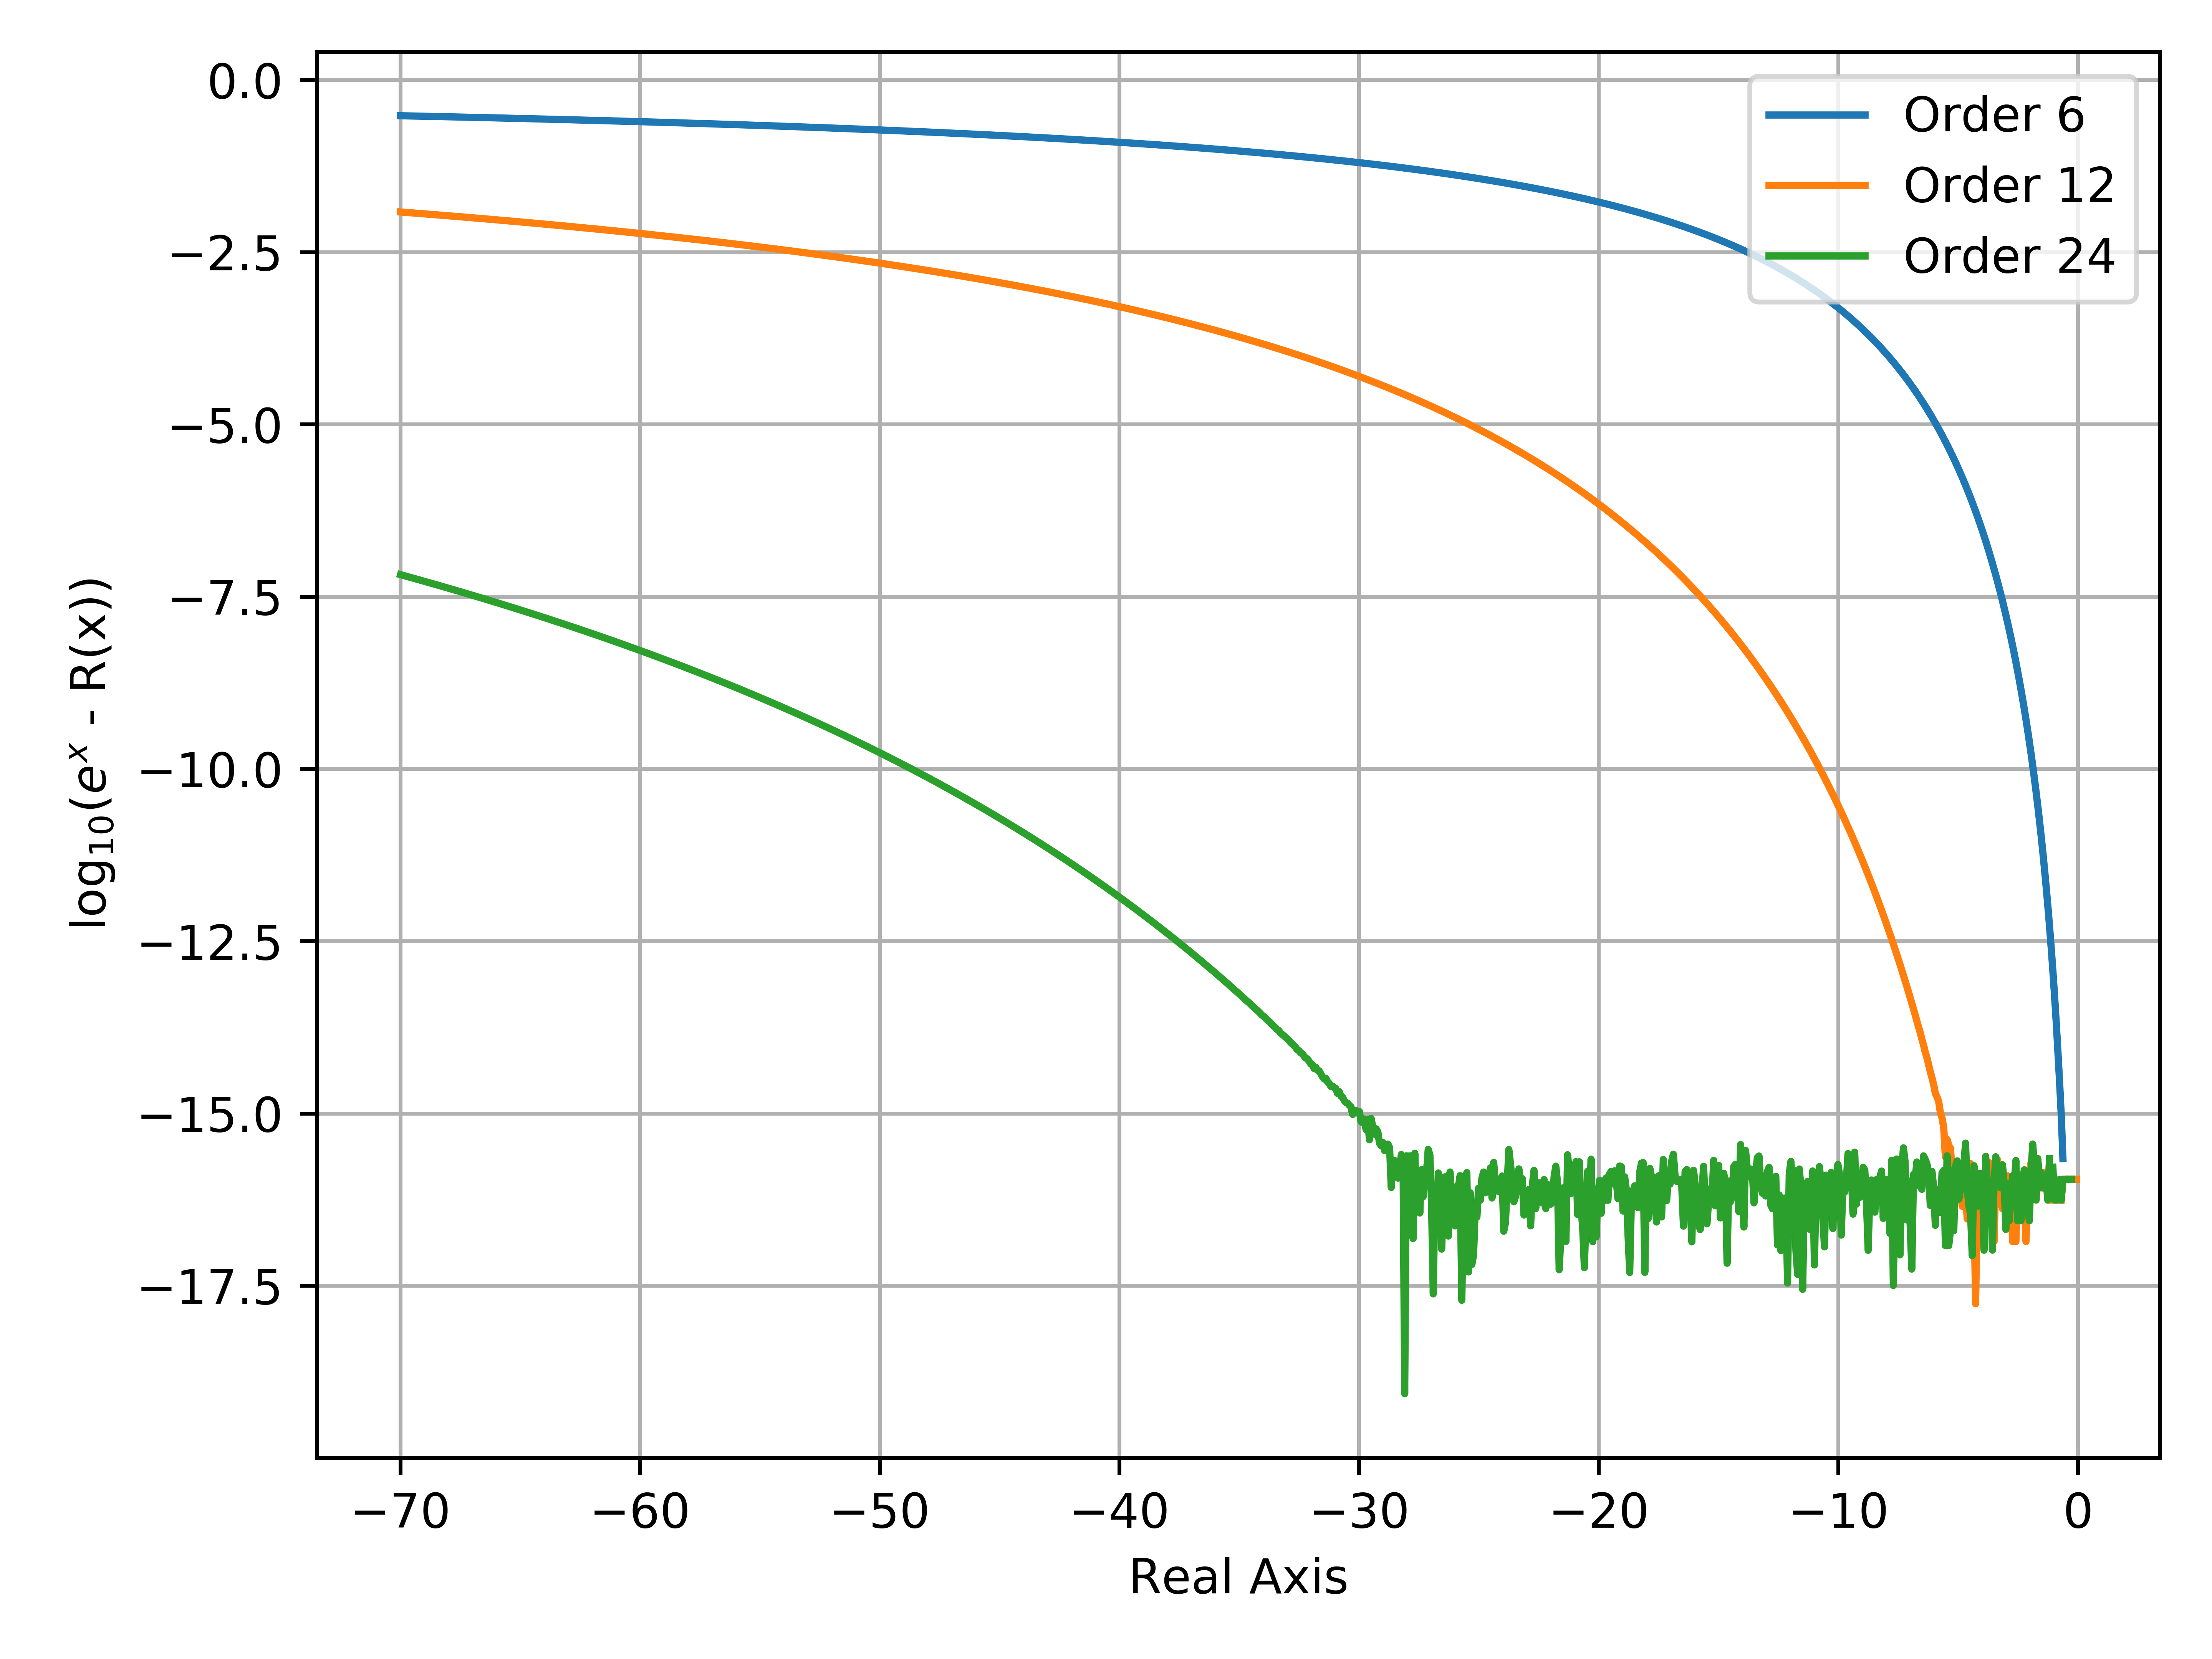
\includegraphics[width=5in]{images/padeError.png}\\
  \caption{$\log_{10}|R(x)-e^{x}|$ for the Pad\'e approximation of orders 6, 12 and 24}
  \label{fig:PadeApproxError}
\end{figure} 


\subsection{Scaling and Squaring}
Both Taylor and Pad\'e methods fail to approximate the matrix exponential when $||\boldsymbol{A}||$ or the spread of the eigenvalues is large. This problem is exacerbated when computing $e^{\boldsymbol{A}t}$ for sufficiently large values of $t$. The scaling and squaring method works to fixed these problem by exploiting the property

\begin{equation*}
    e^{\boldsymbol{A}} = \big( e^{\boldsymbol{A}/m}\big)^{m}
    \label{eq:scalingAndSquaring},
\end{equation*}

\noindent $m$ is a scalar chosen to be $2^{\alpha}$ where $\alpha$ is the number of times the matrix is squared \cite{moler2003}. This property is commonly used for methods based on the Pad\'e approximation. Plugging Equation \ref{eq:scalingAndSquaring} into the Pad\'e approximation gives,

\begin{equation}
    e^{\boldsymbol{A}} = (e^{2^{-\alpha}\boldsymbol{A}})^{2^{\alpha}} \approx R_{p,q}(2^{-\alpha}\boldsymbol{A})^{2^{\alpha}}
\end{equation}

Moler and Van Loan \cite{moler2003} derived an error analysis for choosing the proper value of $\alpha$ based on $||\boldsymbol{A}||$. As noted by Higham \cite{higham2005}, this derivation contained weaknesses. Moler assumed that the matrix norm needed to be less than one half ($||\boldsymbol{A}|| < 1/2$) but Higham proved that this was not the case. Higham further showed that the required minimal matrix norm is different for each order of the Pad\'e implementation. Above this norm, a higher order Pad\'e approximation would be required, or matrix scaling would need to be take place. One other weakness was the derivation of their error bound. It was designed to be easily computable, which resulted in their error bound not being sharp \cite{higham2005}. When the error bound is not sharp, then it is possible to overscale the matrix, resulting in a loss of accuracy. Higham described two algorithms to resolve the overscaling problem found in \cite{higham2005} and \cite{higham2009}. Reference \cite{higham2009} is an updated algorithm to the one described in reference \cite{higham2005}, which works to fix the overscaling problem. 

%\begin{table}[t]
%   \caption{\label{tab:scalingSquaringOptimalValues} Summary of optimal Pad\'e orders and required matrix multiplications \cite{higham2005}}
%   \centering
%   \begin{tabular}{c| cccccccccc}
%   \hline
%   $m$ & 1 & 2 & 3 & 4 & 5 & 6 & 7 & 8 & 9 & 10\\
%   \hline 
%    $\theta_{m}$ & 3.7e-8 & 5.3e-4 & 1.5e-2 & 8.5e-2 & 2.5e-1 & 5.4e-1 & 9.5e-1 & 1.5e0 & 2.1e0 & 2.8e0 \\
%   \hline
%   $\pi_{m}$ & 0 & 1 & 2 & 3 & 3 & 4 & 4 & 5 & 5 & 6 \\
%   \hline
%   \end{tabular}

%   \vspace*{4 mm}
   
%   \begin{tabular}{c| ccccccccccc}
%   \hline
%   $m$ & 11 & 12 & 13 & 14 & 15 & 16 & 17 & 18 & 19 & 20 & 21\\
%   \hline 
%    $\theta_{m}$ & 3.6e0 & 4.5e0 & 5.4e0 & 6.3e0 & 7.3e0 & 8.4e0 & 9.4e0 & 1.1e1 & 1.2e1 & 1.3e1 & 1.4e1 \\
%   \hline
 %  $\pi_{m}$ & 6 & 6 & 6 & 7 & 7 & 7 & 7 & 8 & 8 & 8 & 8 \\
 %  \hline
 %  \end{tabular}
%\end{table}



\subsection{Solutions Based on the Cauchy Integral Formula}
This method is based on transforming the matrix exponential into the complex plane using the Cauchy integral formula.  The matrix exponential becomes,

\begin{equation}
	e^{\boldsymbol{A}} = \frac{1}{2\pi i}\int_{\Gamma} e^{z}(z\boldsymbol{I} - \boldsymbol{A})^{-1}dz,
	\label{eq:cauchyExp}
\end{equation}

\noindent where $\boldsymbol{A}$ is analytic inside the closed contour $\Gamma$ that winds once around the eigenvalues of $\boldsymbol{A}$ \cite{pusaThesis} \cite{pusa2011} \cite{Trefethen2006}. In practice, it is often required to evaluate the action of the matrix exponential on vector $\boldsymbol{v}$, this leads to evaluating,

\begin{equation}
	e^{\boldsymbol{A}}\boldsymbol{v} = \frac{1}{2\pi i}\int_{\Gamma} e^{z}(z\boldsymbol{I} - \boldsymbol{A})^{-1}\boldsymbol{v}dz.
	\label{eq:cauchyExpVector}
\end{equation}

\noindent When evaluating Equations \ref{eq:cauchyExp} or \ref{eq:cauchyExpVector} it is vital to select a contour that encloses the spectrum of $\boldsymbol{A}t$. If this is not done, then the approximation is inaccurate. There are a number of ways to solve Equations \ref{eq:cauchyExp} or \ref{eq:cauchyExpVector} which involve knowing the nature of the spectrum of the transition matrix $\boldsymbol{A}t$. 

\subsubsection{Direct Implementation of a Contour Function}
If one knows the eigenvalue of the transition matrix then one can choose a contour $\Gamma$ that encloses them. The simplest choice would be a circle of radius $R$ centered at point $z_{0}$ \cite{ash2009}.

\begin{equation}
    \phi(\theta) = z_{0} + Re^{i\theta}: 0 \leq \theta \leq 2\pi 
\end{equation}

\noindent Making the substitution $dz = \phi' d\theta$ and making the substitution into Equation \ref{eq:cauchyExp} yields,

\begin{equation}
\begin{split}
    e^{\boldsymbol{A}} 
    & = \frac{1}{2\pi i}\int_{0}^{2\pi} e^{z_{0}-Re^{i\theta}}(z\boldsymbol{I}-\boldsymbol{A})Rie^{i\theta}d\theta \\[3ex]
    & = \frac{1}{2\pi}\int_{0}^{2\pi}(\phi(\theta)-z_{0})(z\boldsymbol{I}-\boldsymbol{A})e^\phi(\theta)d\theta.
\end{split}
\end{equation}

\noindent The integral can then be calculated using a quadrature method. A numerical investigation was conducted by A.H. Ashi et al \cite{ash2009} using the above them by employing a periodic trapezoidal rule. 

\begin{equation*}
    \int_{0}^{2\pi}f(\theta)d\theta \approx \frac{2\pi}{N}\sum_{j=1}^{N}f(\theta_{j}), \quad \theta_{j} = \frac{2\pi j}{N}.
\end{equation*}

\noindent Ashi obtained the following formula for approximating the matrix exponential with $N$ quadrature points, 

\begin{equation}
    e^{\boldsymbol{A}} \approx \frac{1}{N}\sum_{j=1}^{N}(\phi(\theta_{j}) - z_{0})(\phi(\theta_{j})\boldsymbol{I} - \boldsymbol{A})^{-1}e^{\phi(\theta_{j})}.
    \label{eq:ashContour}
\end{equation}


It is important to note that when evaluating Equation \ref{eq:ashContour} that $N$ matrix inversions need to be calculated. However this can be rewritten in the form where the action of the matrix exponential on a vector is calculated. Evaluating Equation \ref{eq:ashContour} would then require solve $N$ number of linear systems, which is generally more adventitious. When the norm of $\boldsymbol{A}t$ becomes larger as you increase $t$ the contour needs to increase to enclose all of the eigenvalues. This leads to increasing the number of quadrature points to maintain accuracy, thus increasing the computational cost \cite{ash2009}. 

\subsubsection{Rational Approximation}
A more generalized method for evaluating the contour integral can be accomplished by choosing an analytic function $\phi(\theta)$ that maps a real line onto the contour. Because the function $e^{\phi(\theta)}$ decreases exponentially as $|\theta| \rightarrow \infty$ the approximation can be truncated to a finite number of quadrature points. When the spectrum of the transition matrix falls on the left hand side of the complex plane close to the real axis then the contour $\Gamma$ denotes a Hankel like contour that winds from $-\infty-0i$ on the lower half-plane and $\infty+0i$ on the upper half-plane. \cite{Trefethen2006}. This allows for the definition of a general contour function that will enclose the eigenvalues on the left hand side of the complex plane around the negative real axis. 

The idea is to solve the contour integral of the form,

\begin{equation}
    I = \frac{1}{2\pi i}\int_{-\infty}^{\infty}e^{\phi(\theta)}f(\phi(\theta))\phi'(\theta)d\theta.
    \label{eq:generalContourIntegral}
\end{equation}

\noindent The trapezoidal approximation with $N$ points to Equation \ref{eq:generalContourIntegral} becomes,

\begin{equation}
    I_{N} = \frac{-i}{N}\sum_{k=1}^{N}e^{z_{k}}f(z_{k})w_{k},
    \label{eq:generalContourIntegralNPoints}
\end{equation}

\noindent where $z_{k} = \phi(\theta_{k})$ and  $w_{k} = \phi'(\theta_{k})$ \cite{Trefethen2006}. It can be shown that Equation \ref{eq:generalContourIntegralNPoints} can be written in the form,

\begin{equation}
    I_{N} = \frac{1}{2\pi i}\int_{C}r(z)f(z)dz, \quad r(z) = \sum_{k=1}^{N}\frac{c_{k}}{z-z_{k}}, \quad c_{k} = iN^{-1}e^{z_{k}}w_{k},
\end{equation}

\noindent where $C$ is a contour that winds around each point $z_{k}$ \cite{Trefethen2006}. The points $z_{k}$ and $c_{k}$ are interpreted as the poles and residues of the rational function. Equation for $r(z)$ is a good approximation to $e^{z}$ near the negative real axis. The error of the quadrature estimate is,

\begin{equation}
    I - I_{N} = \frac{1}{2\pi i}\int_{\Gamma'} \big(e^{z} - r(z)\big)f(z)dz.
\end{equation}{}

\noindent For a contour function $\phi(\theta)$ the goal is to find the rational function $r(z)$ that minimizes the error. 

Trefethen noted three contour functions to $\Gamma$, two of the three are presented here \cite{Trefethen2006}. The simplest contour function is a parabola defined by, 

\begin{equation}
    \phi = N[0.1309 - 0.1194\theta^{2} + 0.2500i\theta]
    \label{eq:parabolicContour}
\end{equation}

\noindent which has a convergence rate of $\mathcal{O}(2.85^{-N} )$. Accuracy of about 14 or more digits can be achieved with N = 32. The approximation of $e^{z}$ on the complex plane is shown in Figure \ref{fig:complexRationalApproxParabola}. The second contour function is that of a hyperbola defined by, 

\begin{equation}
    \phi = 2.246N[1 - \sin(1.1721 - 0.3443i\theta)]
    \label{eq:hyperbolicContour}
\end{equation}

\noindent which has a convergence rate of $\mathcal{O}(3.20^{-N} )$, with an accuracy of about 16 or more digits with N = 32. The same approximation for $e^{z}$ on the complex plane is shown in Figure \ref{fig:complexRationalApproxHyperbola}. Both Figures \ref{fig:complexRationalApproxParabola} and \ref{fig:complexRationalApproxHyperbola} show high levels of accuracy not only on the negative real access but also for a wide region of the left hand side of the complex plane. 

Applying these approximations to real valued scalars or matrices requires half the amount of computational cost, this is because the poles of a rational function with real valued coefficients form conjugate pairs \cite{pusa2011}. For a real scalar, the rational approximation is,

\begin{equation}
    e^{x} \approx r(x) = 2Re\bigg(\sum_{k=1}^{N/2}\frac{c_{k}}{x - z_{k}}\bigg).
\end{equation}

%\FloatBarrier

\begin{figure}[h]
  \centering
  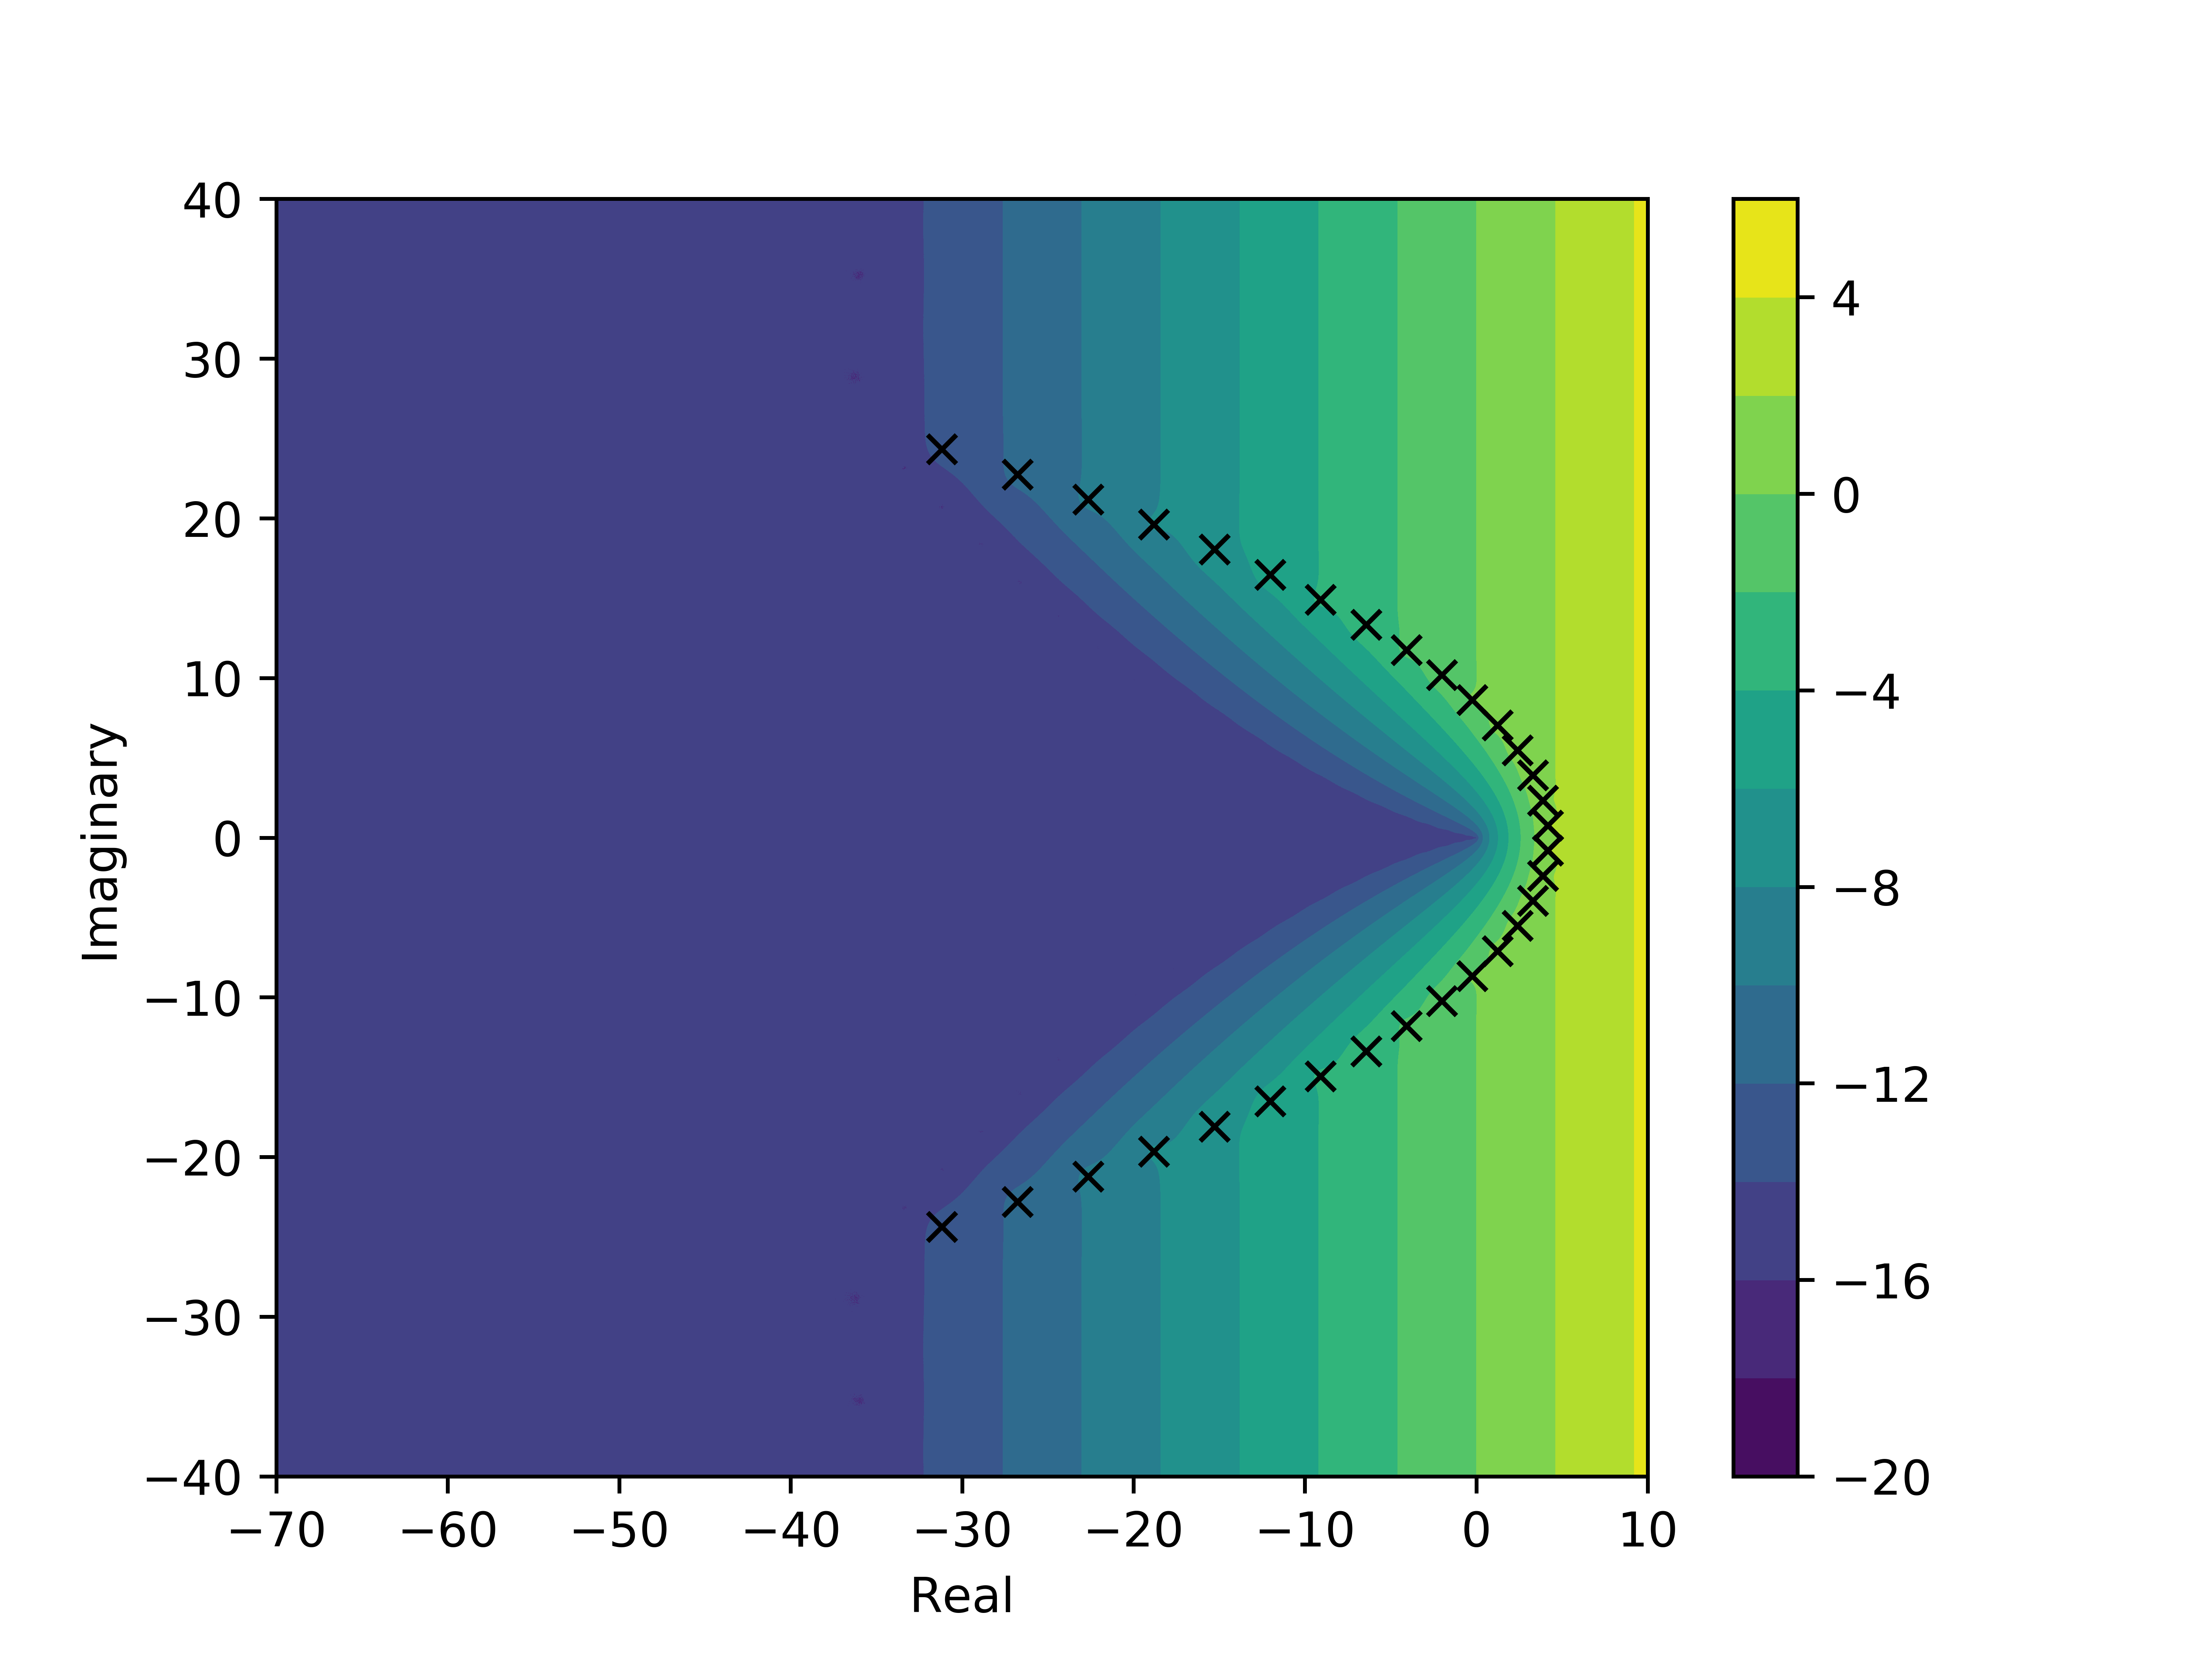
\includegraphics[width=5in]{images/RationApproxParabolicError32.png}\\
  \caption{$\log_{10}|r(z)-e^{z}|$ for N = 32 where the contour is defined by a parabola, Equation \ref{eq:parabolicContour}. Quadrature points are denoted with x's}
  \label{fig:complexRationalApproxParabola}
\end{figure} 

\begin{figure}[h]
  \centering
  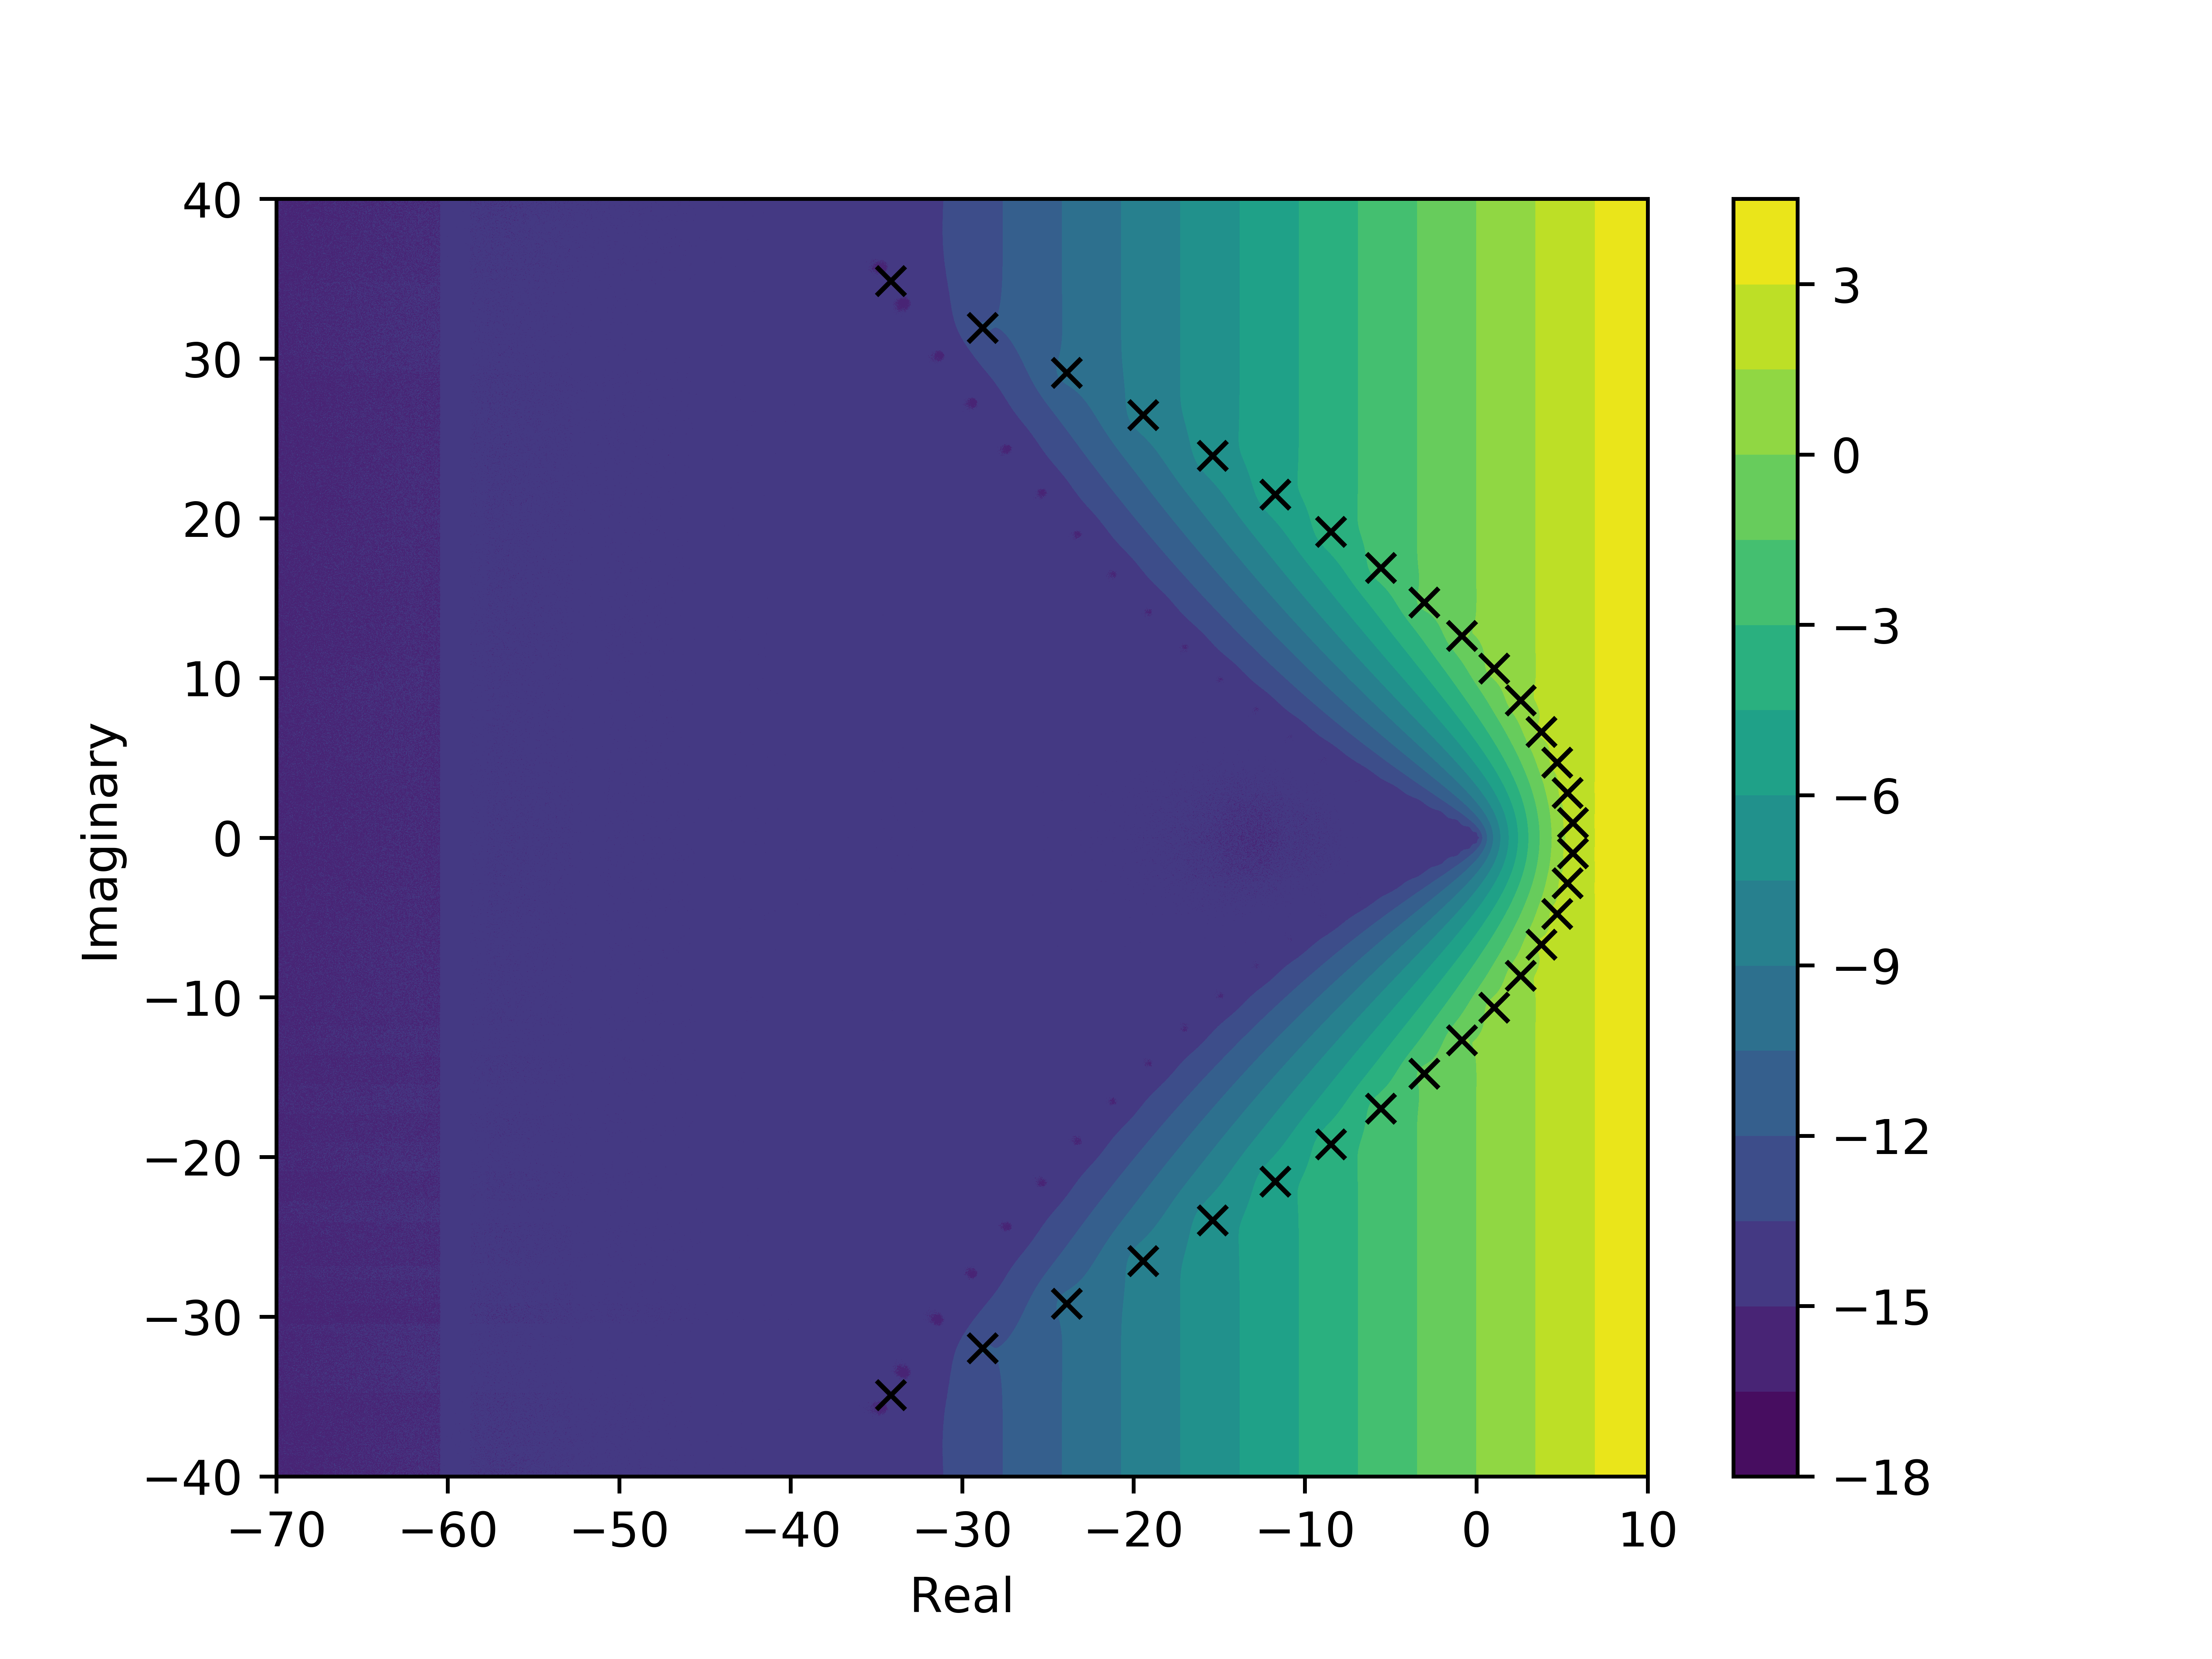
\includegraphics[width=5in]{images/RationApproxHyperbolicError32.png}\\
  \caption{$\log_{10}|r(z)-e^{z}|$ for N = 32 where the contour is defined by a hyperbola, Equation \ref{eq:hyperbolicContour}. Quadrature points are denoted with x's}
  \label{fig:complexRationalApproxHyperbola}
\end{figure} 

%\FloatBarrier




\noindent When applying the rational function to a real valued matrix, the approximation becomes,

\begin{equation}
    e^{\boldsymbol{A}} \approx r(\boldsymbol{A}) = 2Re\bigg(\sum_{k=1}^{N/2}c_{k}(\boldsymbol{A} - z_{k}\boldsymbol{I})^{-1}\bigg),
\end{equation}

\noindent requiring $N/2$ matrix inversions. If instead the action on the matrix exponential on a vector $v$ is calculated, the approximation becomes,

\begin{equation}
    e^{\boldsymbol{A}}\boldsymbol{v} \approx r(\boldsymbol{A})\boldsymbol{v} = 2Re\bigg(\sum_{k=1}^{N/2}c_{k}(\boldsymbol{A} - z_{k}\boldsymbol{I})^{-1}\boldsymbol{v}\bigg),
\end{equation}

\noindent requiring $N/2$ solves of the linear system $\boldsymbol{x} = (\boldsymbol{A} - z_{k}\boldsymbol{I})^{-1}c_{k}\boldsymbol{v}$. It is important to note that each of these linear systems or matrix inversions are independent of one another and can be done in parallel. 

\subsubsection{Best Approximations}
A different approach is to choose a function $r(z)$ that is the best approximation of the exponential function on the negative real axis, doing this bypasses the need for a contour function \cite{pusaThesis} \cite{Trefethen2006}. This method is known as the Chebychev Rational Approximation Method (CRAM) and is done by finding a unique rational function $\hat{r}_{k,k} = \hat{p}_{k}(x)/\hat{q}_{k}(x)$ satisfying 

\begin{equation}
    \epsilon_{k,k} \equiv \sup_{x \in \mathbb{R}_{-}} |\hat{r}_{k,k}(x) - e^{x}| = \inf_{r_{k,k} \in \pi_{k,k}}\bigg\{ \sup_{x \in \mathbb{R}_{-}} |r_{k,k}(x) - e^{x}|\bigg\}.
\end{equation}

\noindent Applying this definition leads to the follows form on the rational approximation,

\begin{equation}
    e^{z} \approx r(z) = c_{0} + \sum_{k=1}^{N}\frac{c_{k}}{z - z_{k}}
\end{equation}


\noindent where $c_{0}$ is the limit at infinity. This formation is the same as the rational approximation with $c_{0} = 0$. The convergence rate for CRAM is of the order $\mathcal{O}(9.28903^{-N} )$, which is remarkably faster than those previously shown. With $N=16$ quadrature points CRAM gives about 15 or more digits of accuracy. Thus the same order of accuracy can be achieved with half the number of quadrature points than the rational approximations defined by contour functions. For a more detailed explanation the CRAM algorithm please refer to Reference \cite{pusaThesis}. 

The difficulty with using the CRAM approximation is finding the coefficient for the rational approximation. For CRAM of order 14 and 16 the rational coefficient can be found in Reference \cite{pusa2011} up to 20 digits. Figure \ref{fig:complexRationalApproxCRAM} shows the accuracy of CRAM to the function $e^{z}$ on the complex plane. Because the rational function was built in such a way to be the best approximation on the negative real axis, the accuracy of CRAM is in a more narrow range of the real axis. For a real values matrix the CRAM algorithm leads to the following solution,

\begin{figure}[t]
  \centering
  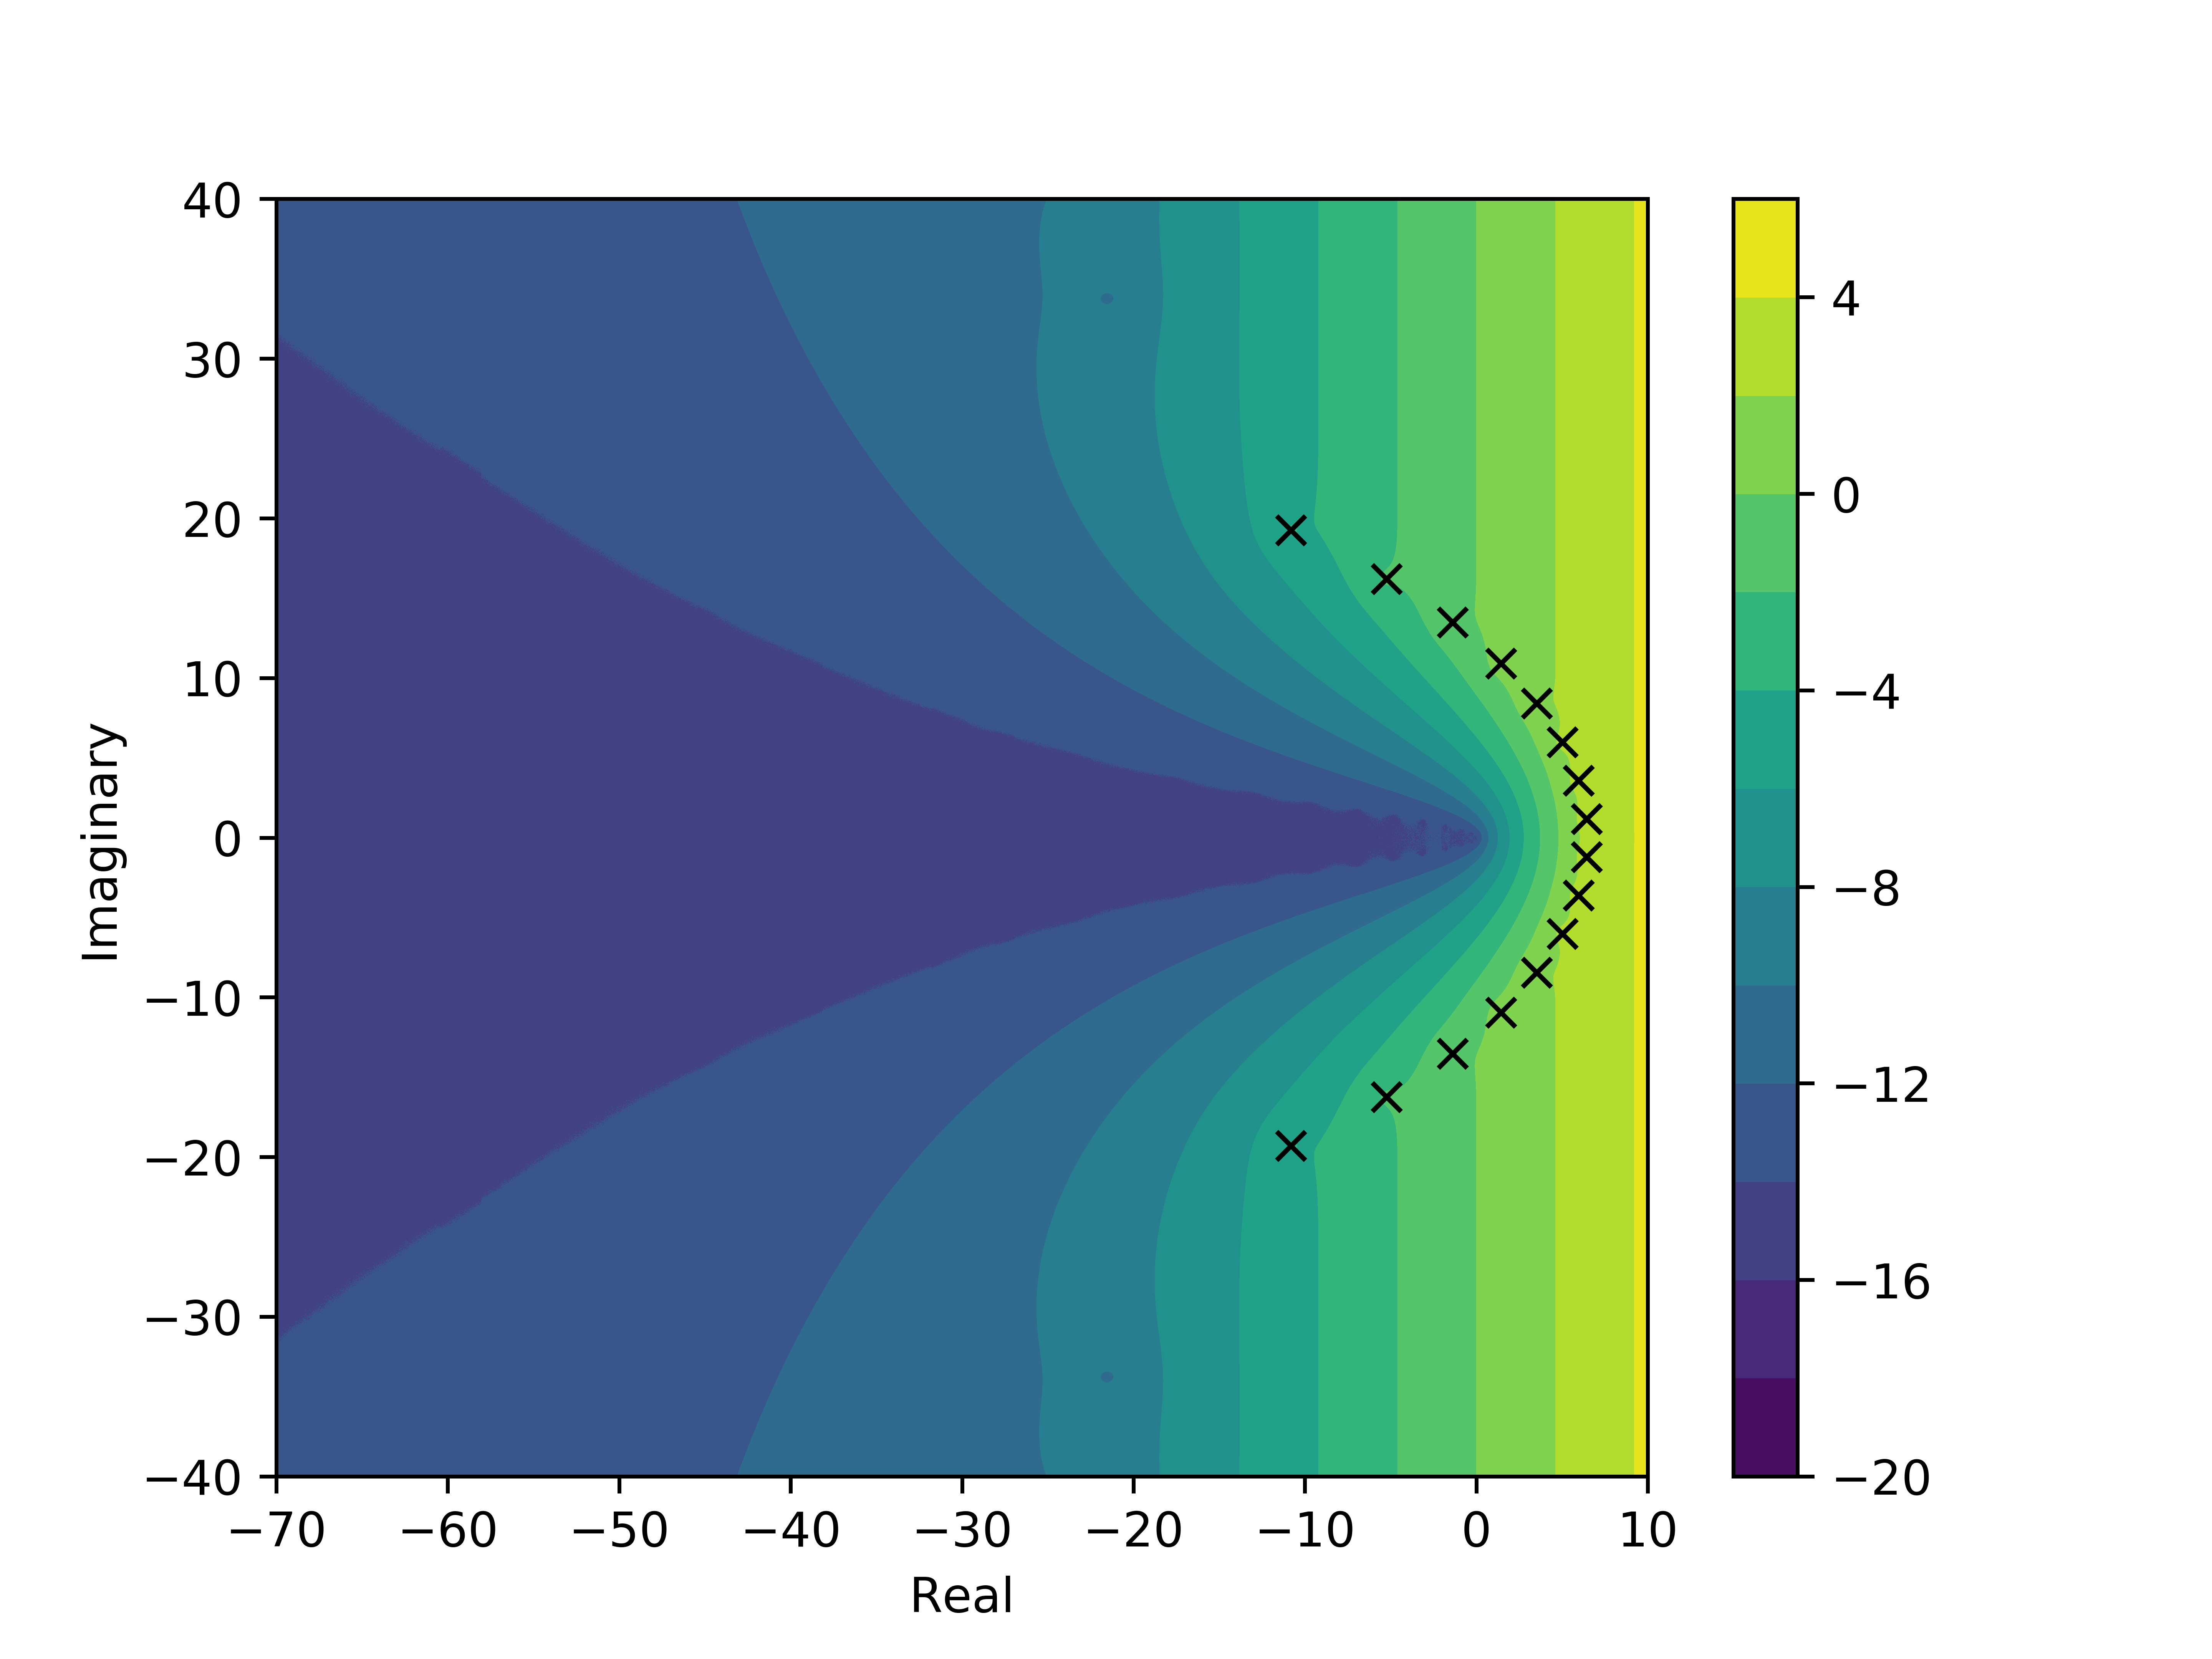
\includegraphics[width=5in]{images/RationApproxCRAMError16.png}\\
  \caption{$\log_{10}|r(z)-e^{z}|$ for CRAM with N = 16. Quadrature points are denoted with x's}
  \label{fig:complexRationalApproxCRAM}
\end{figure} 

\begin{equation}
    e^{\boldsymbol{A}} \approx r(\boldsymbol{A}) = c_{0} + 2Re\Bigg( \sum_{k=1}^{N/2}c_{k}(\boldsymbol{A} - z_{k}\boldsymbol{I})^{-1}\Bigg), 
\end{equation}

\noindent and for the action of the matrix on a vector,

\begin{equation}
    e^{\boldsymbol{A}}\boldsymbol{v} \approx r(\boldsymbol{A})\boldsymbol{v} = c_{0}\boldsymbol{v} + 2Re\Bigg( \sum_{k=1}^{N/2}c_{k}(\boldsymbol{A}t - z_{k}\boldsymbol{I})^{-1}\boldsymbol{v}\Bigg).
    \label{eq:CRAMVector}
\end{equation}




\subsubsection{Krylov Subspace Method}
Krylov subpace approximations are a class of popular methods utilized in sparse matrix algorithms. The idea of Krylov subspace methods is to project the sparse $n \times n$ $\boldsymbol{A}$ matrix into a lower-dimensional subspace. The new lower dimension projection is of size $m \times m$ where $m < n$. Because the matrix is of lower dimension, calculating its matrix exponential becomes much faster. It is important to note that Krylov subspace methods can only be used as an operation on a vector, the direct calculation of the matrix exponential is not possible \cite{saad1992}.  

Consider we want to approximate the matrix exponential as a polynomial of order $m-1$, this takes the form,

\begin{equation}
    e^{\boldsymbol{A}}\boldsymbol{v} \approx p_{m-1}(A)\boldsymbol{v}.
    \label{eq:expPolynomailForm}
\end{equation}

\noindent This approximation is an element of the Krylov subspace defined by,

\begin{equation}
    K_{m} = \text{span}\{\boldsymbol{v}, \boldsymbol{A}\boldsymbol{v}, \boldsymbol{A}^{2}\boldsymbol{v}, ... ,\boldsymbol{A}^{m-1}\boldsymbol{v}\}.
\end{equation}

\noindent For a general non-symmetric matrix the Arnoldi algorithm can be utilized in building the Krylov space \cite{saad1992} \cite{saad1989}. Algorithm \ref{alg:arnoldi} constructs an orthonormal bases $\boldsymbol{V}_{m} = [\boldsymbol{v}_{1}, \boldsymbol{v}_{2}, ... \boldsymbol{v}_{m}]$ of the Krylov subspace, and an $m \times m$ upper Hessenberg matrix. The Arnoldi algorithm produces the following relation,

\begin{equation}
    \boldsymbol{A}\boldsymbol{V}_{m} = \boldsymbol{V}_{m}\boldsymbol{H}_{m} + h_{m+1,m}\boldsymbol{v}_{m+1}\boldsymbol{e}^{T}_{m}
    \label{eq:arnoldiResult}
\end{equation}

\begin{algorithm}
	\caption{Arnoldi} 
	\begin{algorithmic}[1]
	    \State Compute $\boldsymbol{v}_{1} = \boldsymbol{v}/||\boldsymbol{v}||_{2}$
		\For {$j=1,2,\ldots m$}
            \State Compute $\boldsymbol{w} = \boldsymbol{A}\boldsymbol{v}_{j}$
            \For{$i=1,2,\ldots j$}
                \State Compute $h_{i,j} = (\boldsymbol{w},\boldsymbol{v}_{i})$
                \State Compute $\boldsymbol{w} = \boldsymbol{w} - h_{i,j}\boldsymbol{v}_{i}$
            \EndFor
            \State Compute $h_{j+1, j} = ||\boldsymbol{w}||_{2}$ and $\boldsymbol{v}_{j+1} = \boldsymbol{w}/h_{j+1,j}$
		\EndFor
	\end{algorithmic} 
	\label{alg:arnoldi}
\end{algorithm}

\noindent where $\boldsymbol{H}_{m} = \boldsymbol{V}^{T}_{m}\boldsymbol{A}\boldsymbol{V}_{m}$. The Hessenberg matrix $\boldsymbol{H}_{m}$ represents the projection of $\boldsymbol{A}$ on to the Krylov subspace. The approximation in Krylov space is known to be, 

\begin{equation}
    e^{\boldsymbol{A}}\boldsymbol{v} \approx \beta \boldsymbol{V}_{m}e^{\boldsymbol{H}_{m}}\boldsymbol{e}_{1}
    \label{eq:krylovApproxEXP}
\end{equation}

\noindent where $\beta = ||v||_{2}$ \cite{saad1989}. The computation of $e^{
\boldsymbol{H}_{m}}$ becomes much easier because $\boldsymbol{H}_{m}$ is dense and smaller than $\boldsymbol{A}$. After the Krylov approximation is made, a typical method for solving the matrix exponential is used on $e^{\boldsymbol{H}_{m}}$. The quality of this this approximation is exact when $n = m$. This comes from the fact that at step $m$, $h_{m+1,m} = 0$ and Equation \ref{eq:arnoldiResult} becomes,

\begin{equation}
    \boldsymbol{A}\boldsymbol{V}_{m} = \boldsymbol{V}_{m}\boldsymbol{H}_{m}.
\end{equation}

\noindent The Arnoldi process with be exact after $m$ steps when $m$ is greater to or equal to the degree of the minimal polynomial in Equation \ref{eq:expPolynomailForm}. At this point Equation \ref{eq:expPolynomailForm} is exact, however this is unlikely to happen until $m=n$ \cite{saad1992} \cite{saad1989}. 

 The general error associated with applying the approximation in Equation \ref{eq:krylovApproxEXP} can be proven to be,
 
 \begin{equation}
     ||e^{\boldsymbol{A}}\boldsymbol{v} - \beta \boldsymbol{V}_{m}e^{\boldsymbol{H}_{m}}\boldsymbol{e}_{1}||_{2} \leq 2\beta \frac{\rho^{m}e^{\rho}}{m!},
 \end{equation}
 
 \noindent where $\rho = ||A||_{2}$ \cite{saad1992}. The error bounds derived by Saad in \cite{saad1992} can be computed but might not be sharp, especially when the norm of the matrix is large. In practice, a more useful posteriori error can be used to determine the error for applying the Arnoldi algorithm. This error is found after applying the Arnoldi algorithm and is defined by,
 
\begin{equation}
    ||e^{\boldsymbol{A}}\boldsymbol{v} - \beta \boldsymbol{V}_{m}e^{\boldsymbol{H}_{m}}\boldsymbol{e}_{1}||_{2} \approx h_{m+1,m}|\boldsymbol{e}_{m}^{T}\phi(\boldsymbol{H}_{m})\beta \boldsymbol{e}_{1}|,
\end{equation}

\noindent where $\phi(\boldsymbol{A}) = \boldsymbol{A}^{-1}[e^{\boldsymbol{A}} - \boldsymbol{I}]$. This error estimate was found to be sufficient enough for practical applications \cite{saad1992}. 

Krylov subpsace methods are good for approximating the largest eigenvalues of a matrix because of the continued multiplication of $\boldsymbol{A}$ when computing the orthonormal basis \cite{akio2007}. As the spread of the eigenvalues for $\boldsymbol{A}$ increases the accuracy of the Krylove subspace decreases, even as you increase the dimension of the subspace \cite{pusa2010}. 
    \chapter{Application of Matrix Exponential Methods to Burnup Calculations}\label{ch:application}

Chapter \ref{ch:matrixEXPMethods} laid out the fundamental mathematical framework on which Libowski is built. Using this framework, the chemical species transport equation is solved for the time dependent solution of radionuclides in liquid fueled molten salt reactors. This chapter explains the practical application of such methods described in Chapter \ref{ch:matrixEXPMethods} along with the method of lines, to solve the species transport equation. First, the traditional nuclear burnup equations for LWRs are presented, along with their modern day solution in existing reactor depletion codes. Second, the method of lines is presented and used to transform a PDE into a system of coupled ODE's. Finally, some general analysis is conducted on this new governing set of ODE's, to better understand their behavior. This behavior is especially important when choosing one of the matrix exponential solvers described in Chapter \ref{ch:matrixEXPMethods}. 


\section{Application to the Traditional Nuclear Burnup Equations}
 There are many production level software packages which are used to solve these equations, such as SCALE and Serpent. Both of these codes rely on the CRAM method, the reason for this will be described in further detail. 

Nuclear burnup calculations involve solving a set of first order linear ODEs of the form,

\begin{equation}
    \frac{dn_{i}}{dt} = \sum_{j=1}^{N}\bigg(b_{j\rightarrow i}\lambda_{j} + 
    \sum_{k=1}^{K}\gamma_{j\rightarrow i,k}\sigma_{k,j}\phi \bigg)n_{j}(t) - \bigg(\lambda_{i} + \phi\sum_{k=1}^{K} \sigma_{k,i}\bigg)n_{i}(t),
\end{equation}

\noindent which can be written in matrix vector form,

\begin{equation}
    \frac{d\boldsymbol{n}}{dt} = \boldsymbol{A}\boldsymbol{n}, \quad \boldsymbol{n}(t_{0}) = \boldsymbol{n}_{0}, 
    \label{eq:burnup}
\end{equation}

\noindent where, $\boldsymbol{n}(t)$ is the nuclide concentration vector, $\boldsymbol{A}$ is the transition matrix and $\boldsymbol{n}_{0}$ is the initial condition vector. Equation \ref{eq:burnup} has the solution $\boldsymbol{n}(t) = e^{\boldsymbol{A}t}\boldsymbol{n}_{0}$ where $e^{\boldsymbol{A}t}$ was defined in Chapter \ref{ch:matrixEXPMethods}. The transition matrix contains the decay and transmutation coefficients, 

\begin{equation}
    a_{i,i} = -\bigg(\lambda_{i} + \phi\sum_{k=1}^{K} \sigma_{k,i}\bigg),
    \label{eq:diagonalCoeffsTraditionalBurnup}
\end{equation}

\begin{equation}
    a_{i,j\neq i} = b_{j\rightarrow i}\lambda_{j} + 
    \sum_{k=1}^{K}\gamma_{j\rightarrow i,k}\sigma_{k,j}\phi.
    \label{eq:offdiagonalCoeffsTraditionalBurnup}
\end{equation}

\noindent While it is possible to order index the nuclides in any order, the transition matrix becomes nearly upper triangular if the nuclides are indexed by ascending order by their ZAI index defined by $ZAI = 10000Z + 10A + I$, where $Z$ is the atomic number, $A$ is the mass number and $I$ is the isomeric state \cite{pusa2013}.

There are two major matrix properties which influence the accuracy of the matrix exponential algorithms described in Chapter \ref{ch:matrixEXPMethods}, these are the matrix norm and the location of the eigenvalues of the matrix. Series approximations such as Pad\'e are most accurate around the origin, meaning that he norm of the matrix must be small. How small the norm must be depends on the order of the Pad\'e approximation. The $\ell_{1}$ norm the for $\boldsymbol{A}t$ is known to be,

\begin{equation}
    ||\boldsymbol{A}t||_{1} = |t|\hspace{1mm}||\boldsymbol{A}||_{1} \geq |t|\hspace{1mm}\text{max}|a_{i,j}|, 
\end{equation}

\noindent meaning that the norm must be greater than or equal to the absolute value of the max matrix element multiplied by the absolute value of time. Of course, as $t \rightarrow \infty$ the matrix norm does so as well. If one includes half lives on the order of $10^{-6}$s, this would produce a coefficient on the order of $10^{5}$, resulting in $||\boldsymbol{A}t|| \geq 10^{5}$. Because burnup calculations are often taken over long time steps and include isotopes which can greatly increase the norm of the matrix, Pad\'e approximations suffer from complications. In order to utilize these approximations, the matrix needs to be scaled a number of times to reduce the norm to a suitable value. 

Solutions based on the Cauchy integral formula do not have a requirement on the norm of the matrix, but do on the eigenvalues. In particular the eigenvalues of the transition matrix need to fall in a region enclosed by the contour function. It was noted by Pusa that the eigenvalues of the transition matrix are clustered around the negative real axis \cite{pusa2010}. This makes the CRAM algorithm well suited to solve the system in Equation \ref{eq:burnup}. There are a number of papers discussing the accuracy of CRAM vs many commonly used matrix exponential methods for depletion calculations \cite{isotalo2011} \cite{pusa2010}. Both of these papers showed that CRAM outperformed the methods that were tested.

Utilizing the CRAM algorithm to solve Equation \ref{eq:burnup} requires the evaluation of $N/2$ independent systems of equations, where $N$ is the CRAM order. In order to accurately and efficiently solve these linear systems, the mathematical characteristics of the burnup matrix must be understood. If no nuclides are excluded from the calculation then size of the matrix would be about $2,000 \times 2,000$, depending on the library. For example, the SCALE code uses libraries based on ENDF/B-VII.1 which include data for over 2,200 nuclides \cite{scaleManual}. The number of nuclides makes the system large, however it is sparse with the matrix density only a few percent \cite{pusa2013}. 

The half lives and microscopic cross sections for nuclides can vary significantly causing the magnitude coefficients in the transition matrix to vary from zero to $10^{21}$ \cite{pusa2013}. For example, radioactive decay results in half lives ranging from $10^{-24}$ seconds to billions of years \cite{pusaThesis}. Many iterative solvers with have difficulty dealing with the rounding errors introduced by the coefficients. The resulting system will also have eigenvalues with extremely small and large eigenvalues. Iterative solves that rely on Krylov subspace methods become disadvantageous for solving such systems, because of the spectral properties of the matrix \cite{pusa2013}. In order to achieve high order of accuracy and stability, direct solvers are chosen over iterative ones. Such solvers include SuperLU or sparse Gaussian elimination with partial pivoting.

\section{Application to MSR Burnup Calculations}
Molten salt reactor depletion calculations differ greatly from traditional nuclear reactors due to the fact that the fuel salt travels throughout the reactor loop. The MSR depletion equation is a special form of the species transport equations that involves nuclear reactions and possibly nonlinear chemical kinetics. These chemical interactions can come from reactions within the salt, reactions with fission products and reactor loop materials, phase transitions and sparging operations. Equation \ref{eq:MSRDepletion} is rewritten by moving all terms to the right hand side and by adding a term for the chemical kinetics.

\begin{equation}
\begin{split}
    \frac{\partial \rho_{i}}{\partial t}
    = -\nabla \cdot \rho_{i}(r,t)\boldsymbol{v}
    - &\nabla \cdot j_{i}(r)
    +
    \sum_{j=1}^{N}\frac{M_{i}}{M_{j}}\bigg(b_{j\rightarrow i}\lambda_{j} + 
    \sum_{k=1}^{K}\gamma_{j\rightarrow i,k}\sigma_{k,j}(r)\phi(r,t) \bigg)\rho_{j}(r,t)\\
    &- \bigg(\lambda_{i} + \phi(r,t)\sum_{k=1}^{K} \sigma_{k,i}(r)\bigg)\rho_{i}(r,t) +  f_{c}(\boldsymbol{\rho}, r, T).
\end{split}
    \label{eq:MSRDepletionChemKinetics}
\end{equation}

\noindent where $f_{c}(\boldsymbol{\rho}, r, T)$ is a function that represents the generation of chemical species \textit{i}. This generation can include linear and/or nonlinear terms and is a function of chemical species vector $\boldsymbol{\rho}$, space $r$ and temperature $T$. 

The implementation of Equation \ref{eq:MSRDepletionChemKinetics} is done on a finite volume basis. Each finite volume element is considered a depletion zone, meaning that the neutron flux and microscopic cross sections that were applied to Equation \ref{eq:LWRDepletion} are also applied here. For simplicity, we will assume that $f_{c} = 0$. After applying the volume average species density Equation \ref{eq:MSRDepletionChemKinetics} results in,

\begin{equation}
\begin{split}
    \frac{\partial \overline{\rho}_{i}}{\partial t}
    = \frac{-1}{V}\int_{V}\bigg(\nabla \cdot \rho_{i}(r,t)\boldsymbol{v}
    + &\nabla \cdot j_{i}(r)\bigg)dV
    +
    \sum_{j=1}^{N}\frac{M_{i}}{M_{j}}\bigg(b_{j\rightarrow i}\lambda_{j} + 
    \sum_{k=1}^{K}\gamma_{j\rightarrow i,k}\overline{\sigma}_{k,j}\overline{\phi} \bigg)\overline{\rho}_{j}(t)\\
    &- \bigg(\lambda_{i} + \overline{\phi}\sum_{k=1}^{K} \overline{\sigma}_{k,i}\bigg)\overline{\rho}_{i}(t).
\end{split}
\end{equation}

\noindent Each of the transport terms are more complicated and will be treated with the method of lines by discritizing the spacial variables with a 2D finite volume method.


\subsection{Method of Lines}
The method of lines (MOL) is a general technique for solving PDE's which transforms the spacial dependence into an approximate algebraic expression. All but one dimension is discretized, resulting in a system of ODE's. In many physical problems, the undiscretized variable is time. After MOL is applied then normal analytic or numerical integration techniques can be used to solve the system of ODE's. MOL is a generic scheme and can be applied using methods such as finite difference or finite volume \cite{hamdi2007}. 

The finite volume method is a discretization technique which divides the initial spacial domain into smaller volumes. In each volume (cell), the dependent variable is averaged and assumed to be constant. Each volume connects to one another and allows the species to transport between cells. Volumetric generation terms from nuclear and chemical reactions will be a function of the averaged species concentration, neutron flux and microscopic cross sections in that cell. Next each of the transport operators discretized using a 2-D finite volume method. Each cell volume is fixed and of equal size. A visual representation of an internal finite volume cell is shown in Figure \ref{fig:2DFiniteVolume}

\begin{figure}[htbp]
  \centering
  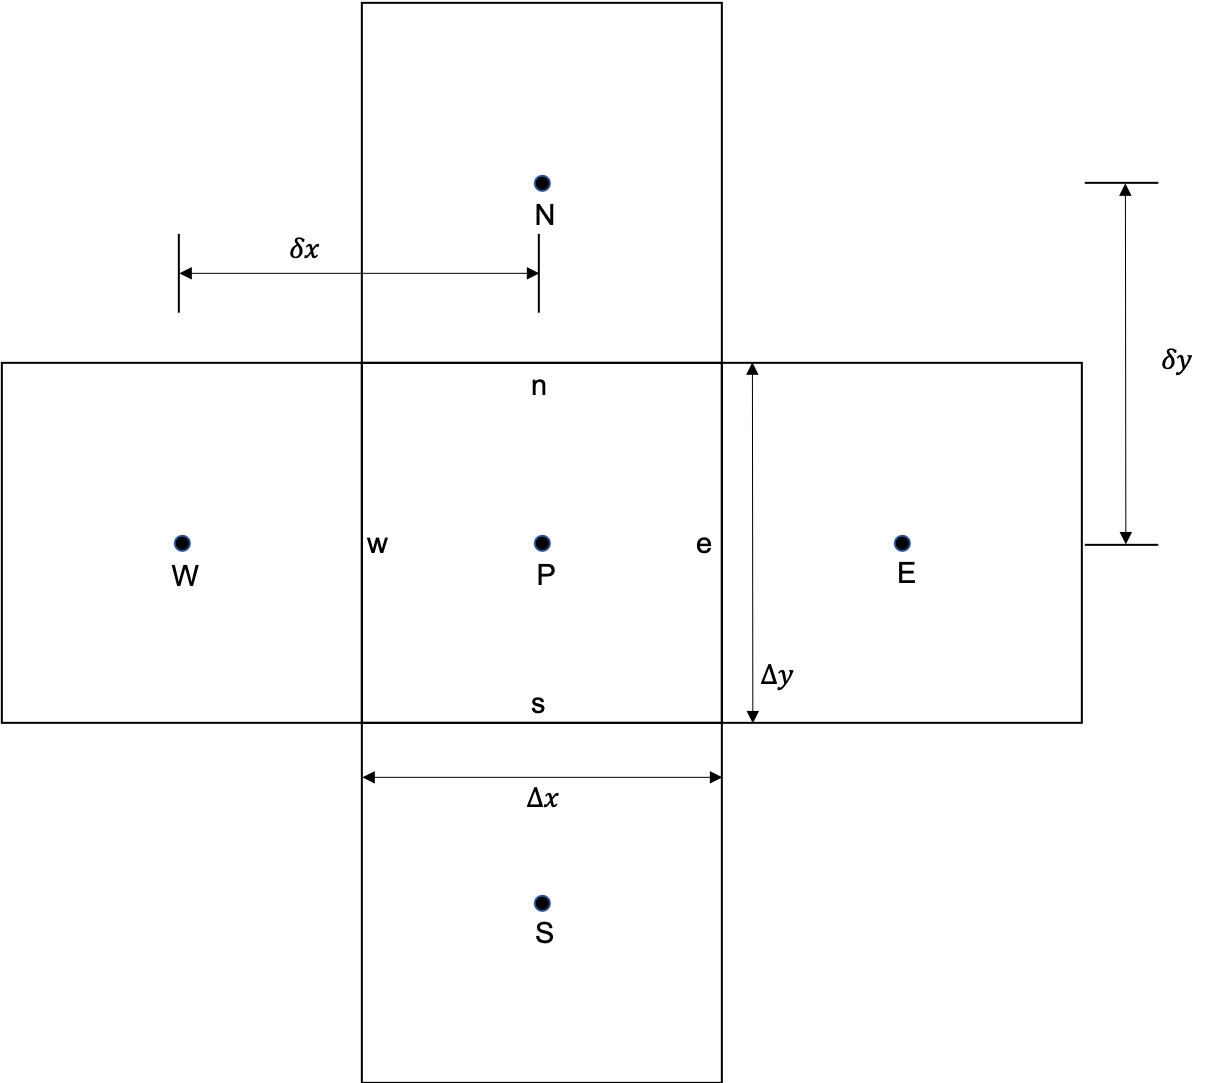
\includegraphics[width=4in]{images/chapter-4/2DFiniteVoluem.png}\\
  \caption{2-D finite volume cell}
  \label{fig:2DFiniteVolume}
\end{figure} 
 
\subsubsection{Diffusion}
The diffusive flux is assumed to follow Fick's law of diffusion for an ideal mixture,

\begin{equation}
    j_{i,x} = -D_{i}\frac{d\rho_{i}}{dx}.
\end{equation}

\noindent In a 2-D system, the diffusion terms results in,

\begin{equation}
    -\int_{V}\nabla \cdot j_{i}dV = -\int_{V}\frac{\partial }{\partial x}\bigg( -D_{i}\frac{\partial \rho_{i}}{\partial x}\bigg)dV - \int_{V}\frac{\partial }{\partial y}\bigg( -D_{i}\frac{\partial \rho_{i}}{\partial y}\bigg)dV.
\end{equation}

\noindent The volume element on a 2-D surface is $dV = dxdy$. To define the diffusive flux into cell P, the diffusion term must be integrated from the West to East wall in the x-direction and from South to North wall in the y-direction \cite{versteeg2007}. This yields,

\begin{equation}
\begin{split}
    \int_{s}^{n}\int_{w}^{e}\frac{\partial }{\partial x}\bigg( D_{i}\frac{\partial \rho_{i}}{\partial x}\bigg)dxdy + \int_{w}^{e}\int_{s}^{n}\frac{\partial }{\partial y}\bigg( D_{i}\frac{\partial \rho_{i}}{\partial y}\bigg)dydx \\ 
    \\
    = D_{e,i}\bigg(\frac{\partial \rho_{i}}{\partial x}\bigg)_{e}\Delta y -D_{w,i}\bigg(\frac{\partial \rho_{i}}{\partial x}\bigg)_{w}\Delta y
    + D_{n,i}\bigg(\frac{\partial \rho_{i}}{\partial y}\bigg)_{n}\Delta x - D_{s,i}\bigg(\frac{\partial \rho_{i}}{\partial y}\bigg)_{s}\Delta x.
\end{split}
\end{equation}

\noindent Each of the first order spacial derivatives are assumed to linearly vary between the cell centered points. The diffusion coefficient are defined to be the average between each of pair of points,

\begin{equation}
    D_{w} =\frac{D_{W} + D_{P}}{2}, \quad D_{e} =\frac{D_{P} + D_{E}}{2}, \quad D_{s} =\frac{D_{S} + D_{P}}{2}, \quad D_{n} =\frac{D_{P} + D_{N}}{2}. 
\end{equation}

\noindent The species diffusive flux across each phase are defined as,

\begin{equation}
\begin{split}
    D_{e,i}\bigg(\frac{\partial \rho_{i}}{\partial x}\bigg)_{e}\Delta y &\approx
    D_{e,i}\bigg(\frac{\rho_{E,i} - \rho_{P,i}}{\delta x}\bigg)\Delta y +
    \mathcal{O}(\Delta x),
    \\
    D_{w,i}\bigg(\frac{\partial \rho_{i}}{\partial x}\bigg)_{w}\Delta y &\approx
    D_{w,i}\bigg(\frac{\rho_{P,i} - \rho_{W,i}}{\delta x}\bigg)\Delta y + \mathcal{O}(\Delta x),
    \\
    D_{n,i}\bigg(\frac{\partial \rho_{i}}{\partial y}\bigg)_{n}\Delta x &\approx
    D_{n,i}\bigg(\frac{\rho_{N,i} - \rho_{P,i}}{\delta y}\bigg)\Delta x +
    \mathcal{O}(\Delta y),
    \\
    D_{s,i}\bigg(\frac{\partial \rho_{i}}{\partial y}\bigg)_{s}\Delta x &\approx
    D_{s,i}\bigg(\frac{\rho_{P,i} - \rho_{S,i}}{\delta y}\bigg)\Delta x +
    \mathcal{O}(\Delta y).
\end{split}
\end{equation}

\noindent Plugging these into the diffusion term in the MSR depletion equation gives,

\begin{equation}
\begin{split}
    \frac{1}{V}\int_{V}\nabla \cdot j_{i} &\approx \frac{D_{e,i}}{\Delta x}\bigg(\frac{\rho_{E,i} - \rho_{P,i}}{\delta x}\bigg) - \frac{D_{w,i}}{\Delta x}\bigg(\frac{\rho_{P,i} - \rho_{W,i}}{\delta y}\bigg) \\ \\
    &+ \frac{D_{n,i}}{\Delta y}\bigg(\frac{\rho_{N,i} - \rho_{P,i}}{\delta y}\bigg) - \frac{D_{s,i}}{\Delta y}\bigg(\frac{\rho_{P,i} - \rho_{S,i}}{\delta y}\bigg).
    \label{eq:diffusionApproximationMSRDepletion}
\end{split}
\end{equation}

\noindent Even though each of the derivative approximations for the flux across each surface where first order, the over all order for the diffusion term at point P is second. It can be shown that the approximation to the second order diffusion term used here, is equivalent to the central difference approximation to the second derivative from a finite difference scheme.

Equation \ref{eq:diffusionApproximationMSRDepletion} can be rearranged into a form which represents the coefficients for an interior node of the transition matrix. For species \textit{i} the coefficients representing diffusion are written as, 

\begin{equation}
    \frac{d \rho_{P}}{dt} = a^{D}_{E}\rho_{E} + a^{D}_{S}\rho_{S} + a^{D}_{P}\rho_{P} + a^{D}_{W}\rho_{W} + a^{D}_{N}\rho_{N},
\end{equation}

\noindent where,

\begin{equation*}
    a^{D}_{E} = \frac{D_{e}}{\Delta x \delta x}, \quad 
    a_{S} = \frac{D_{s}}{\Delta y \delta y}, \quad
    a_{W} = \frac{D_{w}}{\Delta x \delta x}, \quad
    a_{N} = \frac{D_{n}}{\Delta y \delta y},
\end{equation*}

\begin{equation*}
    a^{D}_{P} = - (a^{D}_{E} + a^{D}_{S} + a^{D}_{W} + a^{D}_{N}).
\end{equation*}

\subsubsection{Convection}
Convection-diffusion problems are difficult to numerically model because of the relative strengths each of the operators has on the species transport. These relative strengths can be illustrated by the non-dimensional Peclet number \cite{versteeg2007},

\begin{equation}
    Pe = \frac{\text{Convection}}{\text{Diffusion}} = \frac{\rho v}{D/\delta x}.
\end{equation}

\noindent As convective forces grow relative to the diffusive, the Peclet number gets larger and larger approaching infinity. On the other hand, if the diffusive forces grow at a rate larger than the convective, the Peclet number approaches zero. 

The convective transport term is more complicated and harder to deal with than the diffusion term. Diffusion has no primary direction of flow, it simply cause a species to evenly distribute through a medium through a concentration gradient. Convection on the other hand, has a primary flow direction that is driven by a pressure gradient. One of the major drawbacks of the central differencing scheme is the inability to identify flow direction. In addition to the neglect in identifying the flow direction, the central differencing scheme will cause numerical instability problems for flows with high Peclet number \cite{versteeg2007}. To combat these numerical problems and to handle flow direction, the upwind differencing scheme can be used. 

There are a number of classical differencing schemes such as, first order, power law, and QUICK, each of these will have different orders of accuracy and stability regions. Convection schemes of third order or higher can lead to undershooting or overshooting and applying boundary conditions can be problematic \cite{versteeg2007}. Because of the issues that higher order schemes can have, much development has been done into deriving a class of second-order schemes called total variation diminishing (TVD) that avoid stability and oscillation issues. TVD schemes have the property of preserving monotonicity, meaning that it must not create local extrema and the value of an existing local minimum must be non-decreasing and that of a local maximum must be non-increasing \cite{versteeg2007}. One other consequence of monotonicity preserving scheme is that the total variation of the solution should diminish or remain the same with time. 

The convection term is discretized and represented using a general second order term. First, flow is defined to be positive from cells West to East and South to North and negative in the opposite directions. For positive and negative flows, the convection operators in the x and y-directions are,

\begin{equation}
    \frac{-1}{V}\int_{V}\frac{\partial}{\partial x}(\rho_{i}v) \approx \frac{-1}{\Delta x} \big[ v_{e}\rho_{e,i} - v_{w}\rho_{w,i} \big],
\end{equation}
    
\begin{equation}
    \frac{-1}{V}\int_{V}\frac{\partial}{\partial y}(\rho_{i}v) \approx \frac{-1}{\Delta y} \big[ v_{n}\rho_{n,i} - v_{s}\rho_{s,i} \big].
\end{equation}

\noindent Plugging these in to the convective flux gives,

\begin{equation}
    \frac{-1}{V}\int_{V}\nabla \cdot \rho_{i}(r,t)\boldsymbol{v} \approx 
    \frac{1}{\Delta x} \big[ v_{w}\rho_{w,i} - v_{e}\rho_{e,i} \big] + \frac{1}{\Delta y} \big[ v_{s}\rho_{s,i} - v_{n}\rho_{n,i} \big]
\end{equation}

\noindent These equations remain constant no matter the direction of flow, the change in flow direction is taken into account with the generalized species concentration defined at each cell face. The definitions for the concentrations at each cell face are,

\begin{equation}
\begin{split}
    \text{East Face} \\ 
    \rho_{e} &= \rho_{P} + \frac{1}{2}\Psi(r_{e}^{+})(\rho_{E} - \rho_{P}), \quad v_{e}, v_{w} > 0 \\
    \rho_{e} &= \rho_{E} + \frac{1}{2}\Psi(r_{e}^{-})(\rho_{P} - \rho_{E}), \quad v_{e}, v_{w} < 0 \\
    \label{eq:eastFaceFlux}
\end{split}
\end{equation}

\vspace{-2cm}

\begin{equation}
\begin{split}
    \text{West Face} \\
    \rho_{w} &= \rho_{W} + \frac{1}{2}\Psi(r_{w}^{+})(\rho_{P} - \rho_{W}), \quad v_{e}, v_{w} > 0 \\
    \rho_{w} &= \rho_{P} + \frac{1}{2}\Psi(r_{w}^{-})(\rho_{W} - \rho_{P}), \quad v_{e}, v_{w} < 0 \\
    \label{eq:westFaceFlux}
\end{split} 
\end{equation}

\vspace{-2cm}

\begin{equation}
\begin{split}
    \text{North Face} \\ 
    \rho_{n} &= \rho_{P} + \frac{1}{2}\Psi(r_{n}^{+})(\rho_{N} - \rho_{P}), \quad v_{n}, v_{s} > 0 \\
    \rho_{n} &= \rho_{N} +
    \frac{1}{2}\Psi(r_{n}^{-})(\rho_{P} - \rho_{N}), \quad v_{n}, v_{s} < 0 \\
    \label{eq:northFaceFlux}
\end{split}
\end{equation}

\vspace{-2cm}

\begin{equation}
\begin{split}
    \text{South Face} \\
    \rho_{s} &= \rho_{S} + \frac{1}{2}\Psi(r_{s}^{+})(\rho_{P} - \rho_{S}), \quad v_{n}, v_{s} > 0 \\
    \rho_{s} &= \rho_{P} + \frac{1}{2}\Psi(r_{s}^{-})(\rho_{S} - \rho_{P}), \quad v_{n}, v_{s} < 0 
    \label{eq:southFaceFlux}
\end{split}
\end{equation}

\noindent where $\Psi$ is the flux limiter function and $r$ is the ratio of the upwind side gradient and the downwind side gradient \cite{versteeg2007}. For each cell face, the ratios for positive ($r^{+}$) and negative ($r^{-}$) flows are defined by,

\begin{equation}
    r_{e}^{+} = \bigg( \frac{\rho_{P} - \rho_{W}}{\rho_{E} - \rho_{P}}\bigg), \quad \quad r_{e}^{-} = \bigg( \frac{\rho_{EE} - \rho_{E}}{\rho_{E} - \rho_{P}}\bigg),
\end{equation}

\begin{equation}
    r_{w}^{+} = \bigg( \frac{\rho_{W} - \rho_{WW}}{\rho_{P} - \rho_{W}}\bigg), \quad \quad r_{w}^{-} = \bigg( \frac{\rho_{E} - \rho_{P}}{\rho_{P} - \rho_{W}}\bigg),
\end{equation}

\begin{equation}
    r_{n}^{+} \bigg( \frac{\rho_{P} - \rho_{S}}{\rho_{N} - \rho_{P}} \bigg), \quad \quad r_{n}^{-} = \bigg( \frac{\rho_{NN} - \rho_{N}}{\rho_{N} - \rho_{P}} \bigg),
\end{equation}

\begin{equation}
    r_{s}^{+} = \bigg( \frac{\rho_{S} - \rho_{SS}}{\rho_{P} - \rho_{S}}\bigg), \quad \quad r_{s}^{-} = \bigg(\frac{\rho_{N} - \rho_{P}}{\rho_{P} - \rho_{S}} \bigg).
\end{equation}

The criteria for a scheme to be TVD was derived by Sweby \cite{sweby1984} using the $\Psi - r$ relationship,

\begin{equation}
\begin{split}
    0 < r < 1, &\quad \Psi(r) \leq 2r \\
    r \geq 1, &\quad  \Psi (r) \leq 2.
\end{split}
\end{equation}

\noindent There are a number of flux limiters which can be applied to Equations \ref{eq:eastFaceFlux} - \ref{eq:southFaceFlux}: some of the most popular limiter functions are, Van Leer, Van Albada, Min-Mod, SUPERBEE, QUICK and UMIST. Figure \ref{fig:fluxlimiter} shows the grey shaded region for a second order scheme to be TVD, along with common flux limiter functions. In Figure \ref{fig:fluxlimiter} many of the limiter functions overlap. For the region of $r > 1$ QUICK and UMIST are the exact same and for $r > 5$ UMIST, QUICK and SUPERBEE are the same. 


\begin{figure}[htbp]
  \centering
  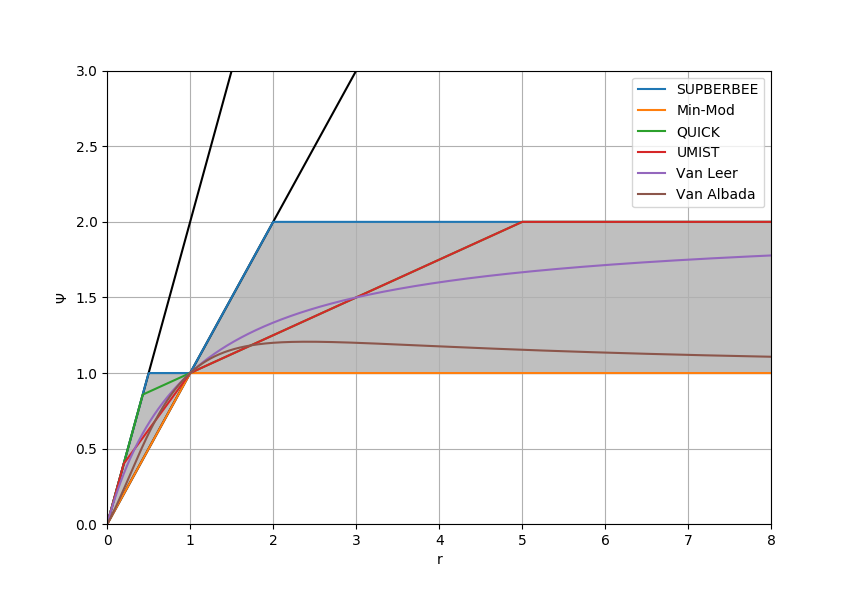
\includegraphics[width=5.5in]{images/chapter-4/CFLlimiterFunctions.png}\\
  \caption{Flux limiter functions on the $\Psi - r$ plane}
  \label{fig:fluxlimiter}
\end{figure} 

TVD schemes can become unstable due to negative main coefficients and they are often reformulated in a different way to maintain numerical stability. One of the ways in which TVD schemes can be reformulated is by deferred corrections. This is an iterative method which breaks apart the convective flux coefficients into its first order upwind difference component and the second order component. The upwind differencing components will still appear in the usual matrix element however, the second order approximations are moved into a source term. The source term for step $n$ is calculated using species densities from step $n-1$. In this way the source term is differed and the convection flux is corrected. This method can be implemented both explicitly or implicitly. If the implicit formulation is used then a method such as Newton must be used to allow the solution to converge at each time step. The explicit method does not require internal iterations at each step but does require small time steps to increase the accuracy and maintain stability for the second order portion. The explicit method is utilized in libowski. For smooth functions this formulation is second order, but reverts back to first order for discontinuous functions.  

Coefficients for the convection flux can also be rewritten in the same way that was done for the diffusion coefficients. The deferred corrections are placed in a source term coefficient. For an interior node of species \textit{i}, the transition matrix will have coefficients representing,

\begin{equation}
    \frac{d \rho_{P}}{dt} = a^{C}_{E}\rho_{E} + a^{C}_{S}\rho_{S} + a^{C}_{P}\rho_{P} + a^{C}_{W}\rho_{W} + a^{C}_{N}\rho_{N} + S^{C},
\end{equation}

\noindent where,

\begin{equation*}
    S^{C} = S_{E}^{C} + S_{S}^{C} + S_{W}^{C} + S_{N}^{C}
\end{equation*}

\begin{equation*}
\begin{split}
    a^{C}_{E} = \max\bigg(\frac{-v_{e}}{\Delta x}, 0\bigg), \quad 
    a^{C}_{S} = \max\bigg(\frac{v_{s}}{\Delta y}, 0\bigg), \quad \\
    a^{C}_{W} = \max\bigg(\frac{v_{w}}{\Delta x}, 0\bigg), \quad
    a^{C}_{N} = \max\bigg(\frac{-v_{n}}{\Delta y}, 0\bigg), \quad 
\end{split}
\end{equation*}

\begin{equation*}
    a_{P}^{C} = -(a_{E}^{C} + a_{S}^{C} + a_{W}^{C} + a_{N}^{C})
\end{equation*}

\begin{equation*}
    S^{C}_{E} = \frac{v_{e}}{2\Delta x}\bigg[(1-\alpha_{e})\Psi(r_{e}^{-}) - \alpha_{e}\Psi(r_{e}^{+})\bigg](\rho_{E} - \rho_{P}), \quad \substack{\alpha_{e} = 0, \quad v_{e} < 0\\
    \\
    \alpha_{e} = 1, \quad v_{e} > 0}
\end{equation*}

\begin{equation*}
    S^{C}_{S} = \frac{v_{s}}{2\Delta y}\bigg[(1-\alpha_{s})\Psi(r_{s}^{-}) - \alpha_{s}\Psi(r_{s}^{+})\bigg](\rho_{S} - \rho_{P}), \quad \substack{\alpha_{s} = 0, \quad v_{s} < 0\\
    \\
    \alpha_{s} = 1, \quad v_{s} > 0}
\end{equation*}

\begin{equation*}
    S^{C}_{W} = \frac{v_{w}}{2\Delta x}\bigg[(1-\alpha_{w})\Psi(r_{w}^{-}) - \alpha_{w}\Psi(r_{w}^{+})\bigg](\rho_{W} - \rho_{P}), \quad \substack{\alpha_{w} = 0, \quad v_{w} < 0\\
    \\
    \alpha_{w} = 1, \quad v_{w} > 0}
\end{equation*}

\begin{equation*}
    S^{C}_{N} = \frac{v_{n}}{2\Delta y}\bigg[(1-\alpha_{n})\Psi(r_{n}^{-}) - \alpha_{n}\Psi(r_{n}^{+})\bigg](\rho_{N} - \rho_{P}), \quad \substack{\alpha_{n} = 0, \quad v_{n} < 0\\
    \\
    \alpha_{n} = 1, \quad v_{n} > 0}
\end{equation*}



\subsection{Linear Source Terms}
Source terms considered thus far are for nuclear reactions. In this transition matrix they are the same as for traditional nuclear burnup equations and the coefficients were shown in Equations \ref{eq:diagonalCoeffsTraditionalBurnup} and \ref{eq:offdiagonalCoeffsTraditionalBurnup}. Diagonal coefficients correspond to the depletion of a species while off diagonal elements are generation terms. For species \textit{i} is interior cell \textit{P} the coefficients of the transition matrix for linear sources are,

\begin{equation}
    \frac{d \rho_{P,i}}{dt} = a_{P,i}^{LS}\rho_{P,i} + \sum_{j=1, j \neq i}^{N}a_{P,j}^{LS}\rho_{P, j} + \sum S^{C}_{i}
\end{equation}


\noindent These source terms will also include the deferred corrections from a second order upwind flux approximation represented as constant source terms. 

Nuclear reaction rates are calculated in such a way to preserve reaction rates. This is done by integrating over all neutron energies and the volume of the cell. Over a single burn up calculation step all cross sections and the scalar neutron flux is assumed to be constant. Using volume average operators and the multigroup approximation, the neutron flux and microscopic cross section is collapsed into single values for each depletion zone \cite{aarnoThesis}:

\begin{equation}
    \sigma_{k,j} = \frac{\int_{V}\int_{0}^{\infty}\sigma_{k,j}(r,E)\phi(r,E) dEdV}{\int_{V}\int_{0}^{\infty}\phi(r,E) dEdV},
\end{equation}

\begin{equation}
    \phi = \frac{1}{V}\int_{V}\int_{0}^{\infty}\phi(r,E)dEdV.
\end{equation}

\noindent Source terms for nuclear reactions are not calculated inside of libowski. Thus, for nuclear reactions, an external source must provide the cross sections, neutron flux and decay constants already calculated in the correct manner. These reactions are added to the transition matrix and are expressed as:

\begin{equation}
    a^{LS}_{P,i} = \lambda_{i} + \overline{\phi}\sum_{k=1}^{K} \overline{\sigma}_{k,i}, \quad 
    a^{LS}_{P,j} = \frac{M_{i}}{M_{j}}\bigg(b_{j\rightarrow i}\lambda_{j} +
    \sum_{k=1}^{K}\gamma_{j\rightarrow i,k}\overline{\sigma}_{k,j}(r)\overline{\phi} \bigg).
\end{equation}

Both of the mass transport models were implemented by added linear coefficients to the transition matrix. If a single species has the ability to transport from the liquid or the wall or gas phase then that species is duplicated three times. In the cases of Xe, if Xe is allowed to transport to the gas bubbles or the wall then Xe will have three individual species \textit{XeLiq}, \textit{XeGas} and \textit{XeWall}. Xe generated in the liquid from fission would be allowed to transport to the gas bubbles or the wall via terms in the transition matrix which are calculated using the mass transfer models. In addition to the mass transfer coefficient, scalar variables such as temperature, interfacial area, gas void fraction and Henry's Law coefficients are required to compute the transition coefficient. 

For species $i$ the following relations represent the mass transfer model for cases when the species exist on the wall or in the liquid:

\begin{equation}
    \frac{d\rho_{i, \text{wall}}}{dt} = \frac{kA}{V}(\rho_{i, \text{liquid}} - \rho_{i,\text{wall}}) \quad \quad \text{Species exist on wall},
\end{equation}

\begin{equation}
    \frac{d\rho_{i, \text{liquid}}}{dt} = \frac{kA}{V}(\rho_{i,\text{wall}} - \rho_{i,\text{liquid}}) \quad \quad \text{Species exist in liquid},
\end{equation}

\noindent where $A$ is the wall area [m$^2$], $V$ is the cell volume [m$^3$] and $k$ is the mass transfer coefficient [m/s]. It is often to express $A/V$ as the interfacial area concentration.The mass transfer coefficient and wall area concentration have to be set by the user when creating the model. In the transition matrix, these coefficients are expressed as:

\begin{equation}
    a^{LS}_{P,i, \text{wall}} = -\frac{kA}{V}, \quad 
    a^{LS}_{P,j, \text{liquid}} = \frac{kA}{V}.
\end{equation}

\begin{equation}
    a^{LS}_{P,i, \text{liquid}} = -\frac{kA}{V}, \quad 
    a^{LS}_{P,j, \text{wall}} = \frac{kA}{V}.
\end{equation}

\noindent In some situations an infinite sink approximation may be appropriate \cite{kedl1972}. This assumes that the species build up on the wall will not influence the mass transfer rate to the wall, reducing the model to: 

\begin{equation}
    \frac{d\rho_{i, \text{wall}}}{dt} = \frac{kA}{V}\rho_{i,\text{liquid}},
\end{equation}

\begin{equation}
    \frac{d\rho_{i, \text{liquid}}}{dt} = -\frac{kA}{V}\rho_{i,\text{liquid}}.
\end{equation}

Gas transport is implemented in a similar way to wall deposition however, the transition coefficient is more complex. Starting with the flux across the bubble interface:

\begin{equation}
    j = k_{l}(\rho^{l}_{*} - \rho^{l}_{\text{bulk}}).
\end{equation}

\noindent where $\rho^{l}_{*}$ is calculated using the gas phase concentration and $\rho^{l}_{\text{bulk}}$ is the liquid phase concentration. Starting with Henry's law for ideal systems, the concentration of gas species $i$ dissolved in the liquid phase is calculated to be:

\begin{equation}
    C_{i} = H_{i}P_{i},
\end{equation}

\noindent where $H_{i}$ is the Henry's law coefficient [kg/Pa/m$^3$] and $P_{i}$ is the partial pressure [Pa] of species $i$. A gas phase species partial pressure is required to calculate the amount of gas dissolved in the liquid. For an ideal gas, the partial pressure can be related to the gas phase mass density starting with the ideal gas law:

\begin{equation}
    P = \frac{nRT}{V}.
\end{equation}

\noindent where $n$ is moles of gas [mol], R is ideal gas constant [m$^3$Pa/mole/K], and T is temperature [K]. Dalton's law says that the total in the gas phase is equal to a summation of the partial pressures of each individual gas component:

\begin{equation}
    P_{\text{total}} = P_{1} + P_{2} + P_{3} ... = \sum_{i=1}^{N} P_{i}, 
\end{equation}

\noindent where partial pressure $P_{i} = P_{\text{total}}x_{i}$ and $x_{i}$ is the mole fraction of species $i$ in the gas phase. Combining Dalton's law and the ideal gas law gives a relation for the partial pressure:

\begin{equation}
    P_{i} = \frac{nRT}{V}\frac{n_{i}}{n} = \frac{n_{i}RT}{V}. 
\end{equation}

\noindent In libowski, species concentrations are solved for mass density in the entire cell volume however, volume in the ideal gas law is for the gas phase. These two volumes are related using the gas void fraction, $V_{\text{gas}} = V_{\text{cell}}\alpha_{\text{gas}}$. Using the volume relation and the molar mass $MM_{i}$ [g/mol] of the gas, the partial pressure of gas $i$ in terms of mass density [kg/m$^3$] is:

\begin{equation}
    P_{i} = \frac{1000RT}{\alpha_{\text{gas}}MM_{i}}\rho_{i}^{g}. 
\end{equation}

\noindent Plugging this relation into Henry's law gives the equilibrium concentration of gas dissolved in the liquid in terms of mass density in the gas phase:

\begin{equation}
    \rho_{*,i}^{l} = \frac{1000H_{i}RT}{\alpha_{\text{gas}}MM_{i}}\rho_{i}^{g}
\end{equation}

\noindent For species $i$ the following relations represent the mass transfer model for cases when the species exist in the gas bubbles or the liquid:

\begin{equation}
    \frac{d\rho_{i, \text{gas}}}{dt} = \frac{kA}{V}\bigg(\rho_{i,\text{liquid}} - \frac{1000H_{i}RT}{\alpha_{\text{gas}}MM_{i}}\rho_{i, \text{gas}}\bigg) \quad \quad \text{Species exist in gas},
\end{equation}

\begin{equation}
    \frac{d\rho_{i, \text{liquid}}}{dt} = \frac{kA}{V}\bigg(\frac{1000H_{i}RT}{\alpha_{\text{gas}}MM_{i}}\rho_{i, \text{gas}} - \rho_{i,\text{liquid}}\bigg) \quad \quad \text{Species exist in liquid},
\end{equation}

\noindent where $k$ is the mass transfer coefficient [m/s] and $A$ is the interfacial area of the gas phase [m$^2$]. Again, the interfacial area concentration $A/V$ is set by the user. In the transition matrix, these coefficients are expressed as:

\begin{equation}
    a^{LS}_{P,i, \text{gas}} = -\frac{kA}{V}\frac{1000H_{i}RT}{\alpha_{\text{gas}}MM_{i}}, \quad 
    a^{LS}_{P,j, \text{liquid}} = \frac{kA}{V}.
\end{equation}

\begin{equation}
    a^{LS}_{P,i, \text{liquid}} = -\frac{kA}{V}, \quad 
    a^{LS}_{P,j, \text{gas}} = \frac{kA}{V}\frac{1000H_{i}RT}{\alpha_{\text{gas}}MM_{i}}.
\end{equation}

\subsection{Treatment of Boundary Conditions}
Dirichlet and Neumann boundary conditions can be easily implemented by the use of "ghost" cells. Ghost cells are cell which are placed outside the boundary of our domain and will allow for a scalar value or the derivative of a scalar value to be set at the boundary of the domain. For example, take a 2-D example of the species transport equation. The differential equation for node $P$ would be,

\begin{equation}
    \frac{d\rho}{dt} = a_{E}\rho_{E} + a_{S}\rho_{S} + a_{P}\rho_{P} + a_{N}\rho_{N} + a_{W}\rho_{W} + S
\end{equation}

\noindent If $P$ was at the East boundary then a Dirichlet boundary condition means that the value at the cell boundary is fixed $(\rho_{e} = \rho_{b,r}$). Because there is a ghost cell to the East of cell $P$, the boundary value can be implemented using a difference across the two cells,

\begin{equation}
    \rho_{e} = \rho_{b} \approx \frac{\rho_{P} + \rho_{E}}{2}.
\end{equation}

\noindent The species concentration for the East cell is solved for and plugged back in to the differential equation to yield new coefficients for the matrix elements. This same method is used for the top, bottom, left, right and the corners. Let the subscript \textit{b} denote a boundary condition value and let \textit{r}, \textit{l}, \textit{t} and \textit{b} denote the right, left, top and bottom boundaries. Table \ref{tab:dirichletBoundaries} shows the modified coefficients for Dirichlet boundary conditions. 

Neumann boundary conditions are applied in a similar way by approximating the derivative at the boundary using a second order central difference approximation at the boundary. For a the bottom boundary this leads to,

\begin{equation}
    \rho_{b}' \approx \frac{\rho_{P} - \rho_{S}}{\delta y}.
\end{equation}

\noindent The concentration in the south boundary cell is solved for and plugged back into the differential equation. A similar process is done for the top, left, right and corners. The results are shown in Table \ref{tab:newmannBoundaries} for the modified coefficients. A mixture of both of these boundary conditions can be used for each side, although special care needs to be taken with the corners if the boundary conditions are mixed. 

Periodic boundary conditions are applied on either the top and bottom or the left and right. This type of boundary condition can be thought of as folding the rectangular domain creating a cylinder. These are implemented by pointing the cell at one boundary next to the cell at the opposite side. For example, if periodic boundary conditions are applied on the top and bottom and the flow is positive, then what comes out the top enters at the bottom. In this way, flow loops can be modeled.

\begin{table}[htbp]
    \caption{\label{tab:dirichletBoundaries} Modified Coefficients for Dirichlet Boundaries}
    \centering
    \begin{tabular}{c|c|c|c|c|c|c}
    \hline
    \textbf{Boundary location} & \textbf{$a_{E}^{*}$} & \textbf{$a_{S}^{*}$} & \textbf{$a_{P}^{*}$} & \textbf{$a_{N}^{*}$} & \textbf{$a_{W}^{*}$} & \textbf{$S^{*}$} \\ [0.5ex]
    \hline
    \hline
    Bottom & $a_{E}$ & $0$ & $a_{P} - a_{S}$ & $a_{N}$ & $a_{W}$ & $S + 2a_{S}\rho_{bb}$\\ \hline
    Top & $a_{E}$ & $a_{S}$ & $a_{P} - a_{N}$ & $0$ & $a_{W}$ & $S + 2a_{N}\rho_{bt}$ \\ \hline 
    Left & $a_{E}$ & $a_{S}$ & $a_{P} - a_{W}$ & $a_{N}$ & $0$ & $S + 2a_{W}\rho_{bl}$  \\ \hline
    Right & $0$ & $a_{S}$ & $a_{P} - a_{E}$ & $a_{N}$ & $a_{W}$ & $S + 2a_{E}\rho_{br}$  \\ \hline
    Bottom left corner & $a_{E}$ & $0$ & $a_{P} - a_{S} - a_{W}$ & $a_{N}$ & $0$ & $S + 2a_{S}\rho_{bb} + 2a_{W}\rho_{bl}$ \\ \hline
    Bottom right corner & $0$ & $0$ & $a_{P} - a_{S} - a_{E}$ & $a_{N}$ & $a_{w}$ & $S + 2a_{S}\rho_{bb} + 2a_{E}\rho_{br}$ \\ \hline
    Top left corner & $a_{E}$ & $a_{S}$ & $a_{P} - a_{N} - a_{W}$ & $0$ & $0$ & $S + 2a_{N}\rho_{bt} + 2a_{W}\rho_{bl}$ \\ \hline
    Top right corner & $0$ & $a_{S}$ & $a_{P} - a_{N} - a_{E}$ & $0$ & $a_{W}$ & $S + 2a_{N}\rho_{bt} + 2a_{E}\rho_{br}$ \\ \hline
    \end{tabular}
\end{table}

\begin{table}[htbp]
    \caption{\label{tab:newmannBoundaries} Modified Coefficients for Newmann Boundaries}
    \centering
    \begin{tabular}{c|c|c|c|c|c|c}
    \hline
    \textbf{Boundary location} & \textbf{$a_{E}^{*}$} & \textbf{$a_{S}^{*}$} & \textbf{$a_{P}^{*}$} & \textbf{$a_{N}^{*}$} & \textbf{$a_{W}^{*}$} & \textbf{$S^{*}$} \\ [0.5ex]
    \hline
    \hline
    Bottom & $a_{E}$ & $0$ & $a_{P} + a_{S}$ & $a_{N}$ & $a_{W}$ & $S - a_{S}\rho_{bb}'\delta y$\\ \hline
    Top & $a_{E}$ & $a_{S}$ & $a_{P} + a_{N}$ & $0$ & $a_{W}$ & $S - a_{N}\rho_{bt}'\delta y$ \\ \hline 
    Left & $a_{E}$ & $a_{S}$ & $a_{P} + a_{W}$ & $a_{N}$ & $0$ & $S - a_{W}\rho_{bl}'\delta x$  \\ \hline
    Right & $0$ & $a_{S}$ & $a_{P} + a_{E}$ & $a_{N}$ & $a_{W}$ & $S - a_{E}\rho_{br}'\delta x$  \\ \hline
    Bottom left corner & $a_{E}$ & $0$ & $a_{P} + a_{S} + a_{W}$ & $a_{N}$ & $0$ & $S - a_{S}\rho_{bb}'\delta y - a_{W}\rho_{bl}'\delta x$ \\ \hline
    Bottom right corner & $0$ & $0$ & $a_{P} + a_{S} + a_{E}$ & $a_{N}$ & $a_{w}$ & $S - a_{S}\rho_{bb}'\delta y - a_{E}\rho_{br}'\delta x$ \\ \hline
    Top left corner & $a_{E}$ & $a_{S}$ & $a_{P} + a_{N} + a_{W}$ & $0$ & $0$ & $S - a_{N}\rho_{bt}'\delta y - a_{W}\rho_{bl}'\delta x$ \\ \hline
    Top right corner & $0$ & $a_{S}$ & $a_{P} + a_{N} + a_{E}$ & $0$ & $a_{W}$ & $S - a_{N}\rho_{bt}'\delta y - a_{E}\rho_{br}'\delta x$ \\ \hline
    \end{tabular}
\end{table}

\subsection{Application of Matrix Exponential Solvers}
Five different matrix exponential solver are implemented in libowski with the added ability to use the Krylov subspace approximation. Each of these methods were discussed in Chapter \ref{ch:matrixEXPMethods} and algorithms are presented in this section. These methods include three based on Cauchys integral formula and two based on Pad\'e's approximation with scaling and squaring. Because of the  various magnitudes of the transition matrix coefficients, a direct solver is used to solve the linear systems \cite{pusa2013}. The direct solver is Eigens sparse LU decomposition which is based on the SuperLU library \cite{eigen} \cite{superlu99}. Each of the algorithms listed in this paper are shown in Appendix \ref{appen:matexpalg}.

\subsubsection{CRAM}
The biggest problem with using CRAM is obtaining the coefficients for the partial fraction decomposition. These coefficients for order 14 and 16 can be found in Reference \cite{pusa2011}, only order 16 is implemented in libowski. As discussed earlier for Cauchy method of order $N$, $N/2$ number of complex linear systems need to be solved. The general algorithm for a method based on contour integrals in partial fraction decomposition form is shown in Algorithm \ref{alg:cauchy}. Both the Parabolic and Hyperbolic methods used this same algorithm but with different poles and residues. It should be noted that notation for the residues where changed from $c_{k}$ to $\alpha_{k}$ and the residues from $z_{k}$ to $\theta_{k}$. For complex matrices and scalars $\alpha$ and $\theta$ would need to be the same size as the approximation order. Real valued matrices and scalars require half of these coefficients. Because all the matrices here are real, $\alpha$ and $\theta$ are all of size $N/2$. 




\subsubsection{Parabolic and Hyperbolic}
Solutions with the parabolic and hyperbolic contours use Algorithm \ref{alg:cauchy} but with different poles and residues. While methods for evaluating the coefficients for CRAM take a long time and need to be precalculated, the poles and residues for contour functions can be computed when the solver is initialized. Calculating the coefficients requires the contour function ($\phi$), the function derivative ($\phi'$) and the order of the approximation ($N$) Algorithms \ref{alg:parabolicCoeffs} and \ref{alg:hyperbolicCoeffs} in Appendix \ref{appen:matexpalg} show the functions computing the arrays for $\alpha$ and $\theta$ with parabolic and hyperbolic contours. While any order is possible, the default order in libowski is 32. 

\subsubsection{Parallelization of Cauchy Solvers}
As mentioned before, for a given order $N$ of the Cauchy solvers $N/2$ linear systems need to be solved. Each of these systems are independent and can be performed separately. Paralelization takes two general forms: shared and distributed memory. Shared memory archetypes involve using multicore CPUs which have access to the same shared memory. Because of this; all processors have access to the same set of variables and can modify them individually. Distributed memory works by connecting multiple CPUs over a network and having each computer solve a portion of the problem. In this case; each computer has its own copy of the variables required to solve its portion of the problem. Libraries exist which allow programmers the ability to parallelize their code on a high level for each of these two architectures. Open multiprocessing (OpenMP) is used for shared memory and message massing interface (MPI) for distributed memory \cite{openmp} \cite{mpi}. In general OpenMP is easier to implement but less flexible because of the memory requirement. This issue with MPI is that using it on a shared memory device will unnecessarily increase the memory consumption. Because of its inherent flexibility MPI is utilized in parallizing the Cauchy solver in libowski. 

\subsubsection{Pad\'e - Method 1}
The first method bast on the Pad\'e approximation was developed by Nicholas J. Higham and can be found in Reference \cite{higham2005}. Higham developed this algorithm in a similar manner which was done before by Moler and Van Loan \cite{moler2003} by choosing the optimal number of matrix scalings required for the Pad\'e of a certain order. Higham noted that the backward error analysis done by Moler and Van Loan was simple and elegant, however not sharp. Instead of only developing an algorithm based on a numerical error bound, Highman also considered computational cost. The resulting algorithm developed by Highman can be found in Reference \cite{higham2005} and the reader should refer to Highman's paper for further detail in its development. Algorithm \ref{alg:method1} is the algorithm that was developed in the paper, and shows its implementation in libowski. From now it shall be referred to as Pad\'e Method 1. Pad\'e Method's 1 and 2 both rely on functions that are shown in Appendix \ref{appen:matexpalg}. Unlike methods based on contour functions, the Pa\'e method directly computes the matrix exponential. 

\subsubsection{Pad\'e - Method 2}
The second Pad\'e method is a modification of the first Pad\'e method that addresses the weakness in overscaling. Overscaling occurs when a large matrix norm causes a larger than necessary $\alpha$ to be used, leading to decreased accuracy \cite{higham2009}. Al-Mohy and Higham developed this algorithm by inroducing a new sharper truncation error bound, which is likely to help correct the overscaling problem. More information on the new algorithm can be found in Referenence \cite{higham2009}. Algorithm 6.1 from said reference is implemented in libowski and is shown in Algorithm \ref{alg:method2}. There are two helper functions that are used in Algorithm \ref{alg:method2}, these function are defined Appendix \ref{appen:matexpalg} along with Algorithm \ref{alg:method2}. 


\subsubsection{Taylor}
The Taylor algorithms implemented in libowski was taken from Reference \cite{higham2011} for computing $F \approx e^{\boldsymbol{A}t}\boldsymbol{B}$ over a single step, where $\boldsymbol{A} \in \mathbb{C}^{n\times n}$ and $\boldsymbol{B} \in \mathbb{C}^{n\times n_{0}}$. Unlike the Pad\'e methods, the Taylor algorithm does not require the need for linear solves. This was done in an attempt to reduce the computational cost. Three key ideas were employed when developing this algorithm:

\begin{enumerate}
    \item Careful choice of the Taylor series order and scaling parameter, exploiting estimates of $||t{\boldsymbol{A}}^{p}||^{p}$, to keep the backward error suitably bounded while minimizing the computational cost.
    \item Shifting, and optional balancing, to reduce the norm of $\boldsymbol{A}t$.
    \item Premature termination of the truncated Taylor series evaluations.
\end{enumerate}


One of the major components of this algorithm is in picking the optimal Taylor order and scaling parameter. This is accomplished by minimizing the computational cost while choosing the appropriate scaling and squaring parameter to obtain a backwards error below a minimal tolerance. For this algorithm, the parameters function accomplishes this and is shown in Algorithm \ref{alg:taylor_parameters}. This algorithm requires 2 additional parameters $p_{\text{max}}$ and $m_{\text{max}}$, where $m_{\text{max}}$ is the maximum order of the Taylor series. The first parameter $p_{\text{max}}$ is the largest integer such that $p(p - 1) \leq m_{\text{max}} + 1$. For values of $m$ up to 100, $p_{\text{max}}$ are tabulated in table \ref{tab:pmax_mmax_values}. Reference \cite{higham2011} notes that as $m_{\text{max}}$ increases the overall cost of the algorithm decreases however, large values of $m$ can lead to numerical instability. The default parameters, which were recommended by Al-Mohy et al., are $p_{\text{max}} = 8$ and $m_{\text{max}} = 55$.  

 
    \chapter{Results}\label{ch:results}

In chapters \ref{ch:burnupEquations}, \ref{ch:matrixEXPMethods}, \ref{ch:application} the theoretical framework and application for solving mass transport problems in MSRs were developed on a finite volume mesh. Components of the solution strategy are broken in to three general categories:

\begin{enumerate}
    \item Diffusion operator
    \item Convection operator
    \item Time integration
\end{enumerate}

\noindent The first two categories deal with the spatial discretization of the PDE. The third involves the time variance in the solution as its ability to handle volumetric source terms. A number of test are conducted to access the numerical solution of libowski with these three key features in mind. These test aim to explore the accuracy of the libowski and the computation time required to solve such problems. A set of progression problems are defined which explore, diffusion, convection, linear source terms and the combination of each. After this small case studies are performed with a nuclear reactor design in mind which looks at libowskis' ability to handle the types of problems which arrive in the field. These problems include the set of neutron precursors as well as depletion and mass transport with a small selection of radio nuclides. 

In order to test the validity of libowski, the problems which are conducted must have reference solutions to test against. Many of the problems do in fact have analytical solutions while some do not. For those that do not MATLAB is utilized in generating the reference solution. In these cases the transition matrix and initial condition that is generated in libowski is save to a CSV file and read by a MATLAB script. This script then uses the Symbolic tool box to calculate the exponential of the transition matrix using variable precision arithmetic with 64 digits of accuracy. The solution is then converted to IEEE double precision and read in to libowski as the reference solution. While this method is not able to test the accuracy of the diffusion or convection operators, it is able to access the time integration thus overall accuracy of the matrix exponential algorithms. 

Many of the case studies involve a set of isotopes that are referred to as the small and medium sets. These set of isotopes were chosen based on their inclusion in TRITON for cross section evaluation with depletion \cite{scaleManual}. The small case corresponds to \textit{addnux} = -2 and the medium case to \textit{addnux} = 2. Additional isotopes are added to both of these sets to fully include the initial condition for the MSRE salt \cite{MSREbenchmark}. The list of isotopes for the small and medium cases are shown in Appendix , Tables  . One important note about these tables is that indicate which species will have addition mass transport models for wall deposition and gas sparging. In some cases no mass transport is included, resulting in a subset of nuclides which do not include the additional isotopes required to model addition mass transport models. For example if one were to model three species, ${}^{235}$U, ${}^{135}$Xe and ${}^{109}$Ag with no mass transport then the system would only contain these three isotopes. If wall deposition and gas sparging is added for Ag and Xe then the system would contain two addition species ${}^{135}$XeGas and ${}^{109}$AgWall. Making the total number of species five. 

All problems show an error based on a reference solution. For the following results the relative errors are defined as:

\begin{equation*}
    E_{\infty} = \max\bigg(|\hat{u}_{i} - u_{i}|\bigg) \quad \text{For } i = 1, 2, ..., N,
\end{equation*}

\begin{equation*}
    E_{1} = \frac{1}{N}\sum_{i=1}^{N}|\hat{u}_{i} - u_{i}|, \quad \quad E_{2} = \frac{1}{N}\sqrt{\sum_{i=1}^{N}\bigg(|\hat{u}_{i} - u_{i}|\bigg)^{2}},
\end{equation*}

\noindent where $N$ is the number of elements in the solution domain. Some times it is more meaningful to shown an absolute error instead of a relative error. It is explicitly stated in the results weather a relative or absolute difference is used. Run time is also reported for some test and is reported as the wall time for calling the \textit{solve} function. This includes the time to build the matrix, run the solution algorithm and unpack the solution. For problems where multiple time steps are taken, the matrix is rebuilt before each time step to update the deferred correction source term. While these run times are reported with no standard deviation, some changes are to be expected by running the problems multiple times or on different machines. 

Earlier, it was discussed that substepping can increase the accuracy of Cauchy based solvers. For all results shown, unless other wise noted, no substeps are used for either the CRAM, Parabolic or Hyperbolic solvers. For some of the reaction-diffusion-convection problems, substepping does not play a role in increasing the accuracy of the solution but will increase the run time. Exceptions to this will be further discussed in the results. The default orders for the CRAM, Hyperbolic and Parabolic solvers in libowski are 16, 32 and 32 respectively. 

\section{Progression Problems}
\subsection{Problem 1}
The first diffusion problem consist of a 2-D system shown as:

\begin{equation}
    \frac{\partial U}{\partial t} = k\frac{\partial^{2}U}{\partial x^{2}} + k\frac{\partial^{2}U}{\partial y^{2}},
\end{equation}

\noindent on the domain $x \in [0,1]$, $y \in [0,1]$, subject to periodic boundary conditions and initial condition,


\begin{equation}
    U(x,y,0) = \sin(2\pi x)\sin(2\pi y),
\end{equation}

\noindent and solution,

\begin{equation}
    U(x,y,t) = e^{-t}\sin(2\pi x)\sin(2\pi y),
\end{equation}

\noindent with $k = 1/(8\pi^{2}$). The Problem is ran for a total time of 2.0 seconds with the number of cells in the x and y direction being the same [10, 20, 40, 80]. These results are shown in Table \ref{tab:diffusion_problem1_results}. These results show good convergence rates for the $l_{\infty}$ and $l_{1}$ error functions previous described, but not $l_{2}$. While each of the solvers maintained the same error, the run times were drastically different. Run times for each of the solvers is shown in Figure (\ref{fig:runtime_diffusion_one}).

From Figure (\ref{fig:runtime_diffusion_one}) each of the solvers show a monomial relation between the problem size and run time. Both the Parabolic and Hyperbolic solvers have almost the exact same solve time. This is because they have to solve the same number of linear systems. The CRAM solver requires half the number of linear solves, making it about twice as fast. For this example the Taylor solver is the fastest but only slightly beats each of the Cauchy solvers. The Pad\'e solvers scale much more poorly than the other ones. Starting out each of the solvers have a similar run time but as the problem size increases, the Pad\'e methods run times grow at a faster rate. Each of these solvers maintain the same numerical error do the the error being dominated by the spatial discretization error of the diffusion operator. 

The eigenvalues for this problem were found to be clustered on the negative real axis with zero imaginary parts. For the 400 x 400 case, the eigenvalues are shown in Figure \ref{fig:eigenvalues_diffusion_one}.  On exception to this is a positive eigenvalue which is very close to the origin at 6.0396e-14. This positive value only appears in the 400 x 400 case. The other discretizations show the same behavior with the eigenvalues being clustered on the negative real axis but do not show the positive valued eigenvalue a the origin. Due to the relatively long solve times, particularly for the Pad\'e solvers, the Krylov subspace approximation was used to analyze the error and run time. For a spatial resolution of 160 cells in both the x and y direction, results for various subspace dimensions $M$ are shown in Table \ref{tab:diffusion_problem1_results_krylov}. Interestingly, the error associated with reducing the overall dimension of the problem did not change, even though the run time drastically decreased leading to the conclusion that the dimension of the true space is much smaller. 


\FloatBarrier

\begin{table}[p]
   \caption{\label{tab:diffusion_problem1_results} Convergence Rate for Diffusion Problem 1  with Absolute Error}
   \centering
    \scalebox{0.8}{
   \begin{tabular}{cllllllll}
   \hline
    Solver & Cells & E${}_{\infty}$ Rate & E${}_{1}$ Rate & E${}_{2}$ Rate & E${}_{\infty}$ Error & E${}_{1}$ Error & E${}_{2}$ Error & Solve Time (sec)\\
   \hline
   CRAM         &  100 & - & - & - & 4.39e-03 & 1.84e-03 & 2.20e-04 & 8.06e-03 \\ 
   -         &  400 & 2.02 & 2.02 & 2.98 & 1.08e-03 & 4.53e-04 & 2.77e-05 & 5.07e-02 \\ 
   -         & 1600 & 1.97 & 2.01 & 3.00 & 2.76e-04 & 1.13e-04 & 3.48e-06 & 5.37e-01 \\ 
   -         & 6400 & 1.99 & 2.00 & 3.00 & 6.94e-05 & 2.82e-05 & 4.35e-07 & 5.62e+00 \\ 
   \hline
   Parabolic    &  100 & - & - & - & 4.39e-03 & 1.84e-03 & 2.20e-04 & 1.08e-02 \\ 
   -    &  400 & 2.02 & 2.02 & 2.98 & 1.08e-03 & 4.53e-04 & 2.77e-05 & 9.71e-02 \\ 
   -    & 1600 & 1.97 & 2.01 & 3.00 & 2.76e-04 & 1.13e-04 & 3.48e-06 & 1.06e+00 \\ 
   -    & 6400 & 1.99 & 2.00 & 3.00 & 6.94e-05 & 2.82e-05 & 4.35e-07 & 1.10e+01 \\ 
   \hline
   Hyperbolic   &  100 & - & - & - & 4.39e-03 & 1.84e-03 & 2.20e-04 & 1.07e-02 \\ 
   -   &  400 & 2.02 & 2.02 & 2.98 & 1.08e-03 & 4.53e-04 & 2.77e-05 & 9.70e-02 \\ 
   -   & 1600 & 1.97 & 2.01 & 3.00 & 2.76e-04 & 1.13e-04 & 3.48e-06 & 1.05e+00 \\ 
   -   & 6400 & 1.99 & 2.00 & 3.00 & 6.94e-05 & 2.82e-05 & 4.35e-07 & 1.10e+01 \\ 
   \hline
   Pade-method1 &  100 & - & - & - & 4.39e-03 & 1.84e-03 & 2.20e-04 & 6.19e-03 \\ 
   - &  400 & 2.02 & 2.02 & 2.98 & 1.08e-03 & 4.53e-04 & 2.77e-05 & 5.27e-01 \\ 
   - & 1600 & 1.97 & 2.01 & 3.00 & 2.76e-04 & 1.13e-04 & 3.48e-06 & 6.70e+01 \\ 
   - & 6400 & 1.99 & 2.00 & 3.00 & 6.94e-05 & 2.82e-05 & 4.35e-07 & 5.52e+03 \\ 
   \hline
   Pade-method2 &  100 & - & - & - & 4.39e-03 & 1.84e-03 & 2.20e-04 & 1.62e-02 \\ 
   - &  400 & 2.02 & 2.02 & 2.98 & 1.08e-03 & 4.53e-04 & 2.77e-05 & 1.23e+00 \\ 
   - & 1600 & 1.97 & 2.01 & 3.00 & 2.76e-04 & 1.13e-04 & 3.48e-06 & 1.19e+02 \\ 
   - & 6400 & 1.99 & 2.00 & 3.00 & 6.94e-05 & 2.82e-05 & 4.35e-07 & 9.48e+03 \\ 
   \hline
   Taylor       &  100 & - & - & - & 4.39e-03 & 1.84e-03 & 2.20e-04 & 4.83e-03 \\ 
   -      &  400 & 2.02 & 2.02 & 2.98 & 1.08e-03 & 4.53e-04 & 2.77e-05 & 2.20e-02 \\ 
   -      & 1600 & 1.97 & 2.01 & 3.00 & 2.76e-04 & 1.13e-04 & 3.48e-06 & 1.20e-01 \\ 
   -      & 6400 & 1.99 & 2.00 & 3.00 & 6.94e-05 & 2.82e-05 & 4.35e-07 & 7.38e-01 \\ 
   \hline
   \end{tabular}
   }
\end{table}

\clearpage

\begin{figure}[ht]
    \centering
    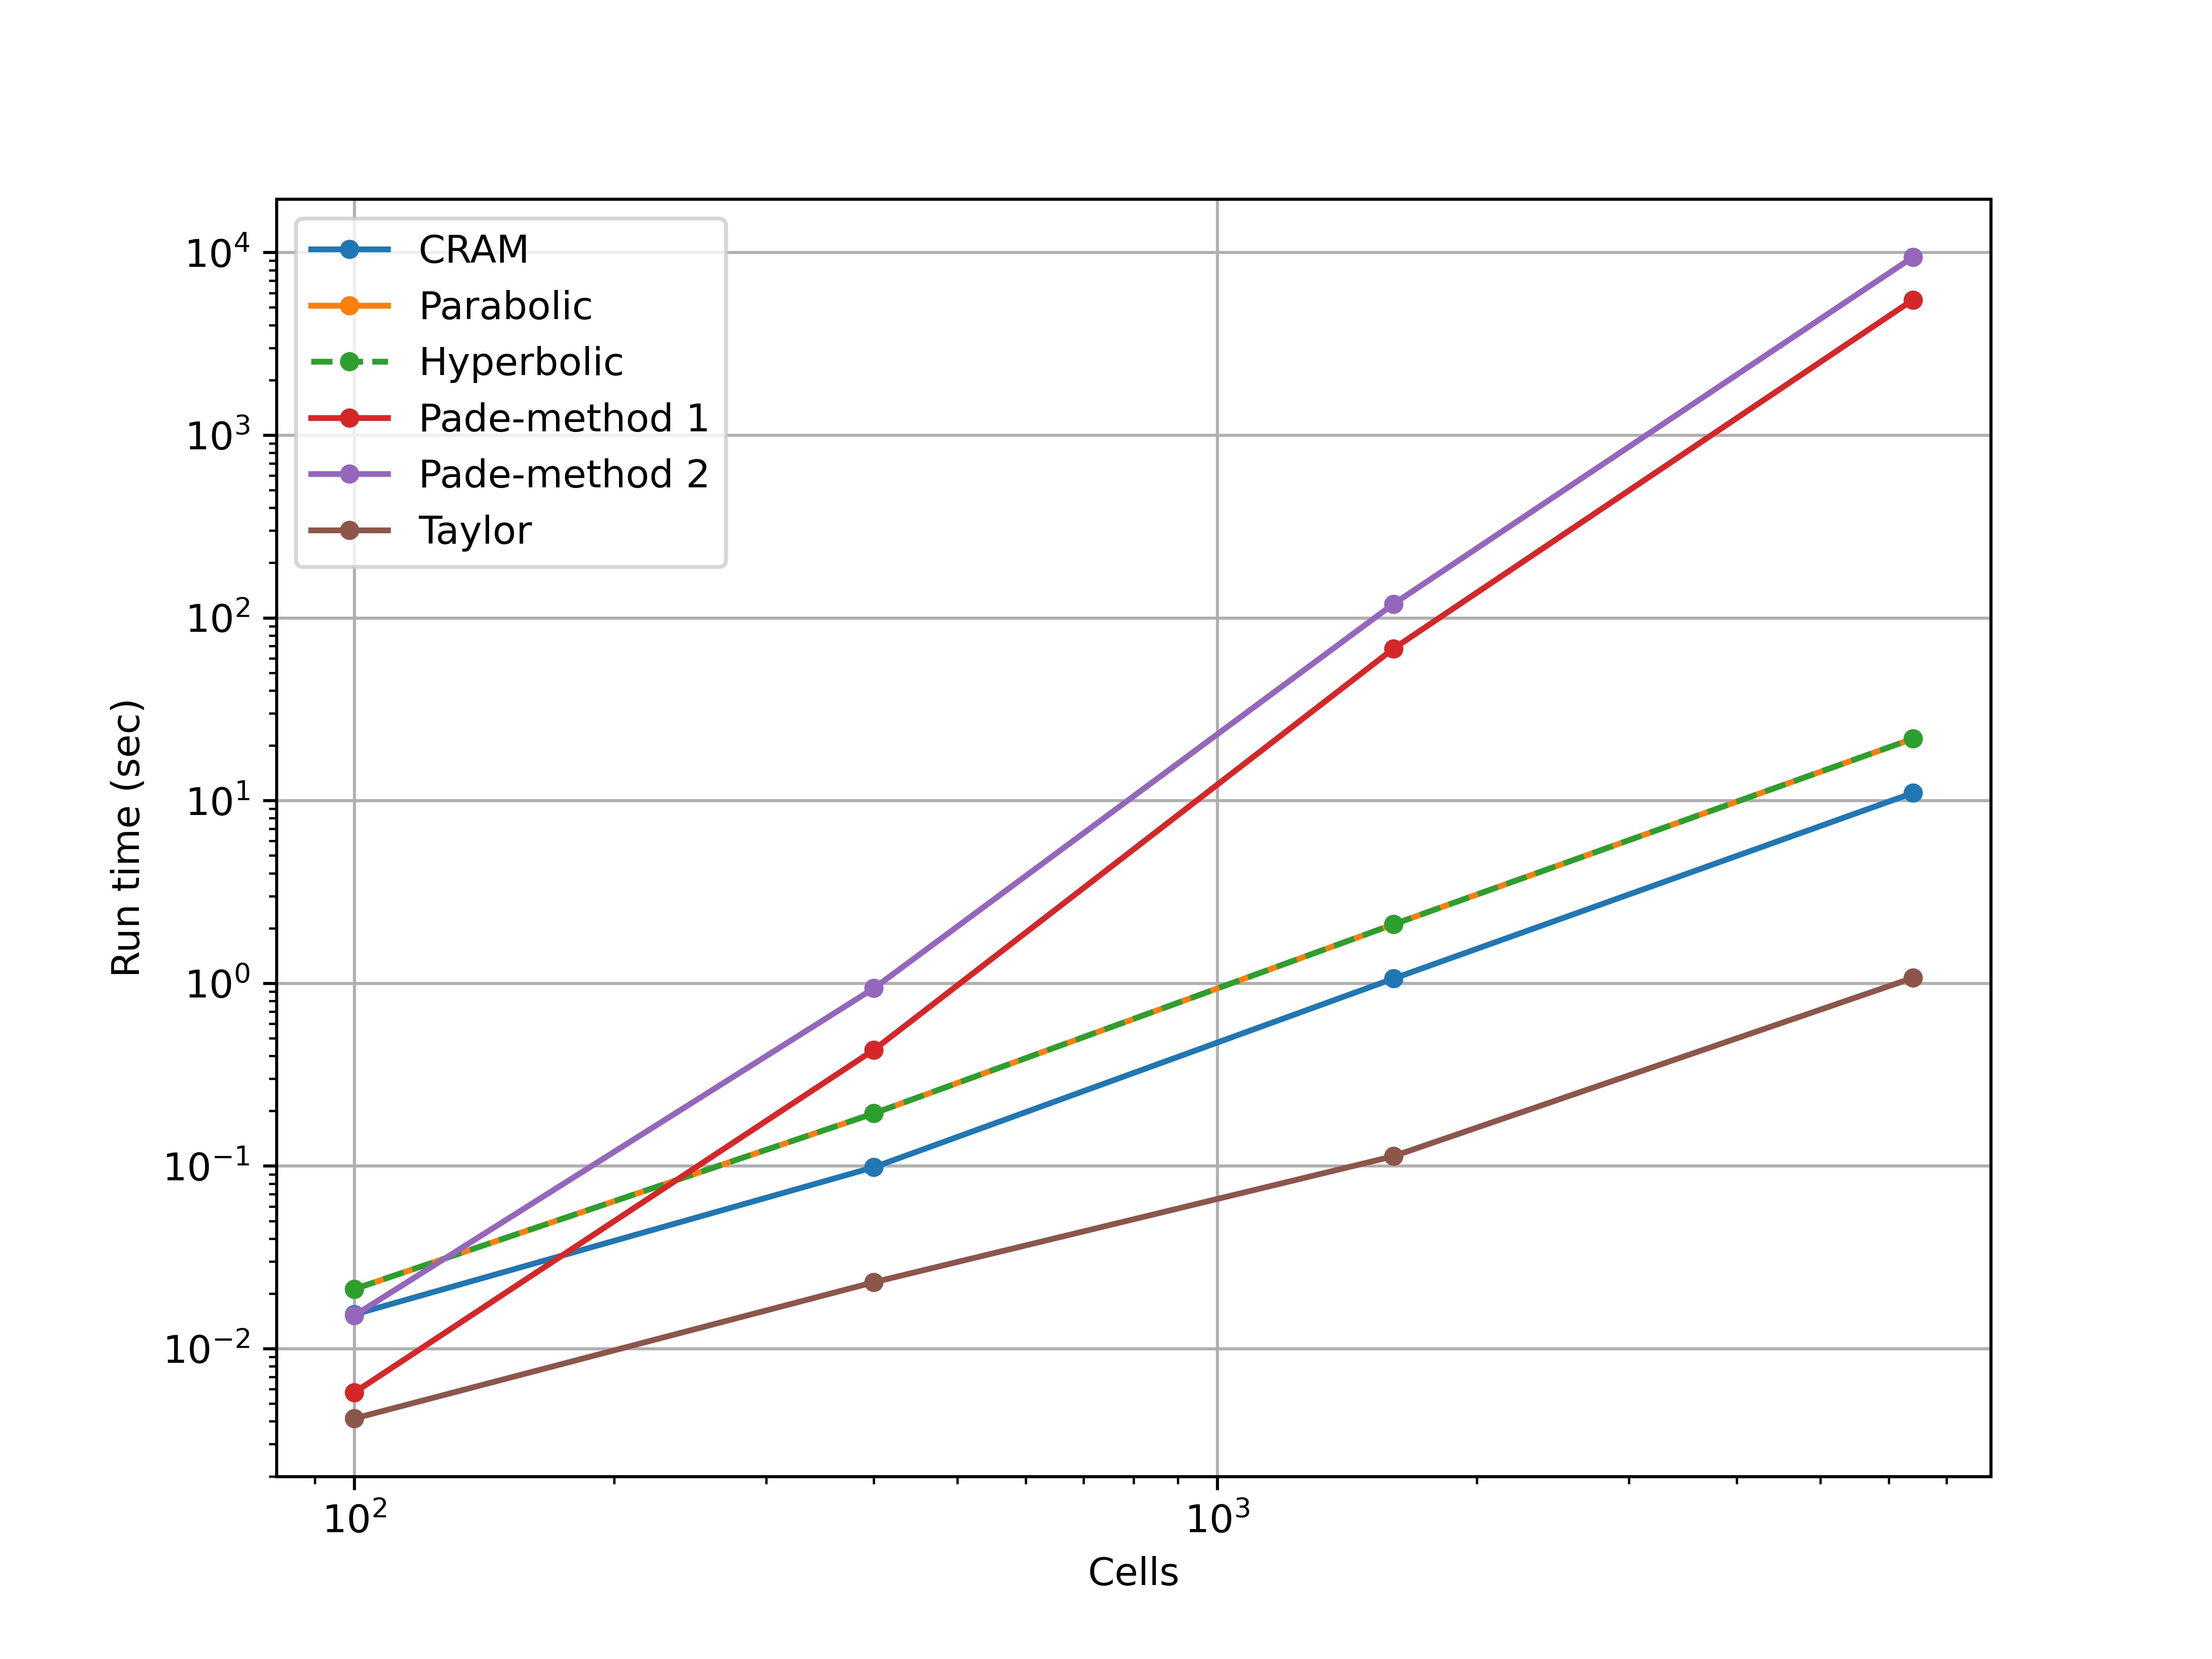
\includegraphics[width=3.9in]{images/chapter-5/progressionProblems/problem1/diffusionProblem1Runtime.png}
    \caption{Run time performance for diffusion problem one}
    \label{fig:runtime_diffusion_one}
\end{figure}

\begin{figure}[hb]
    \centering
    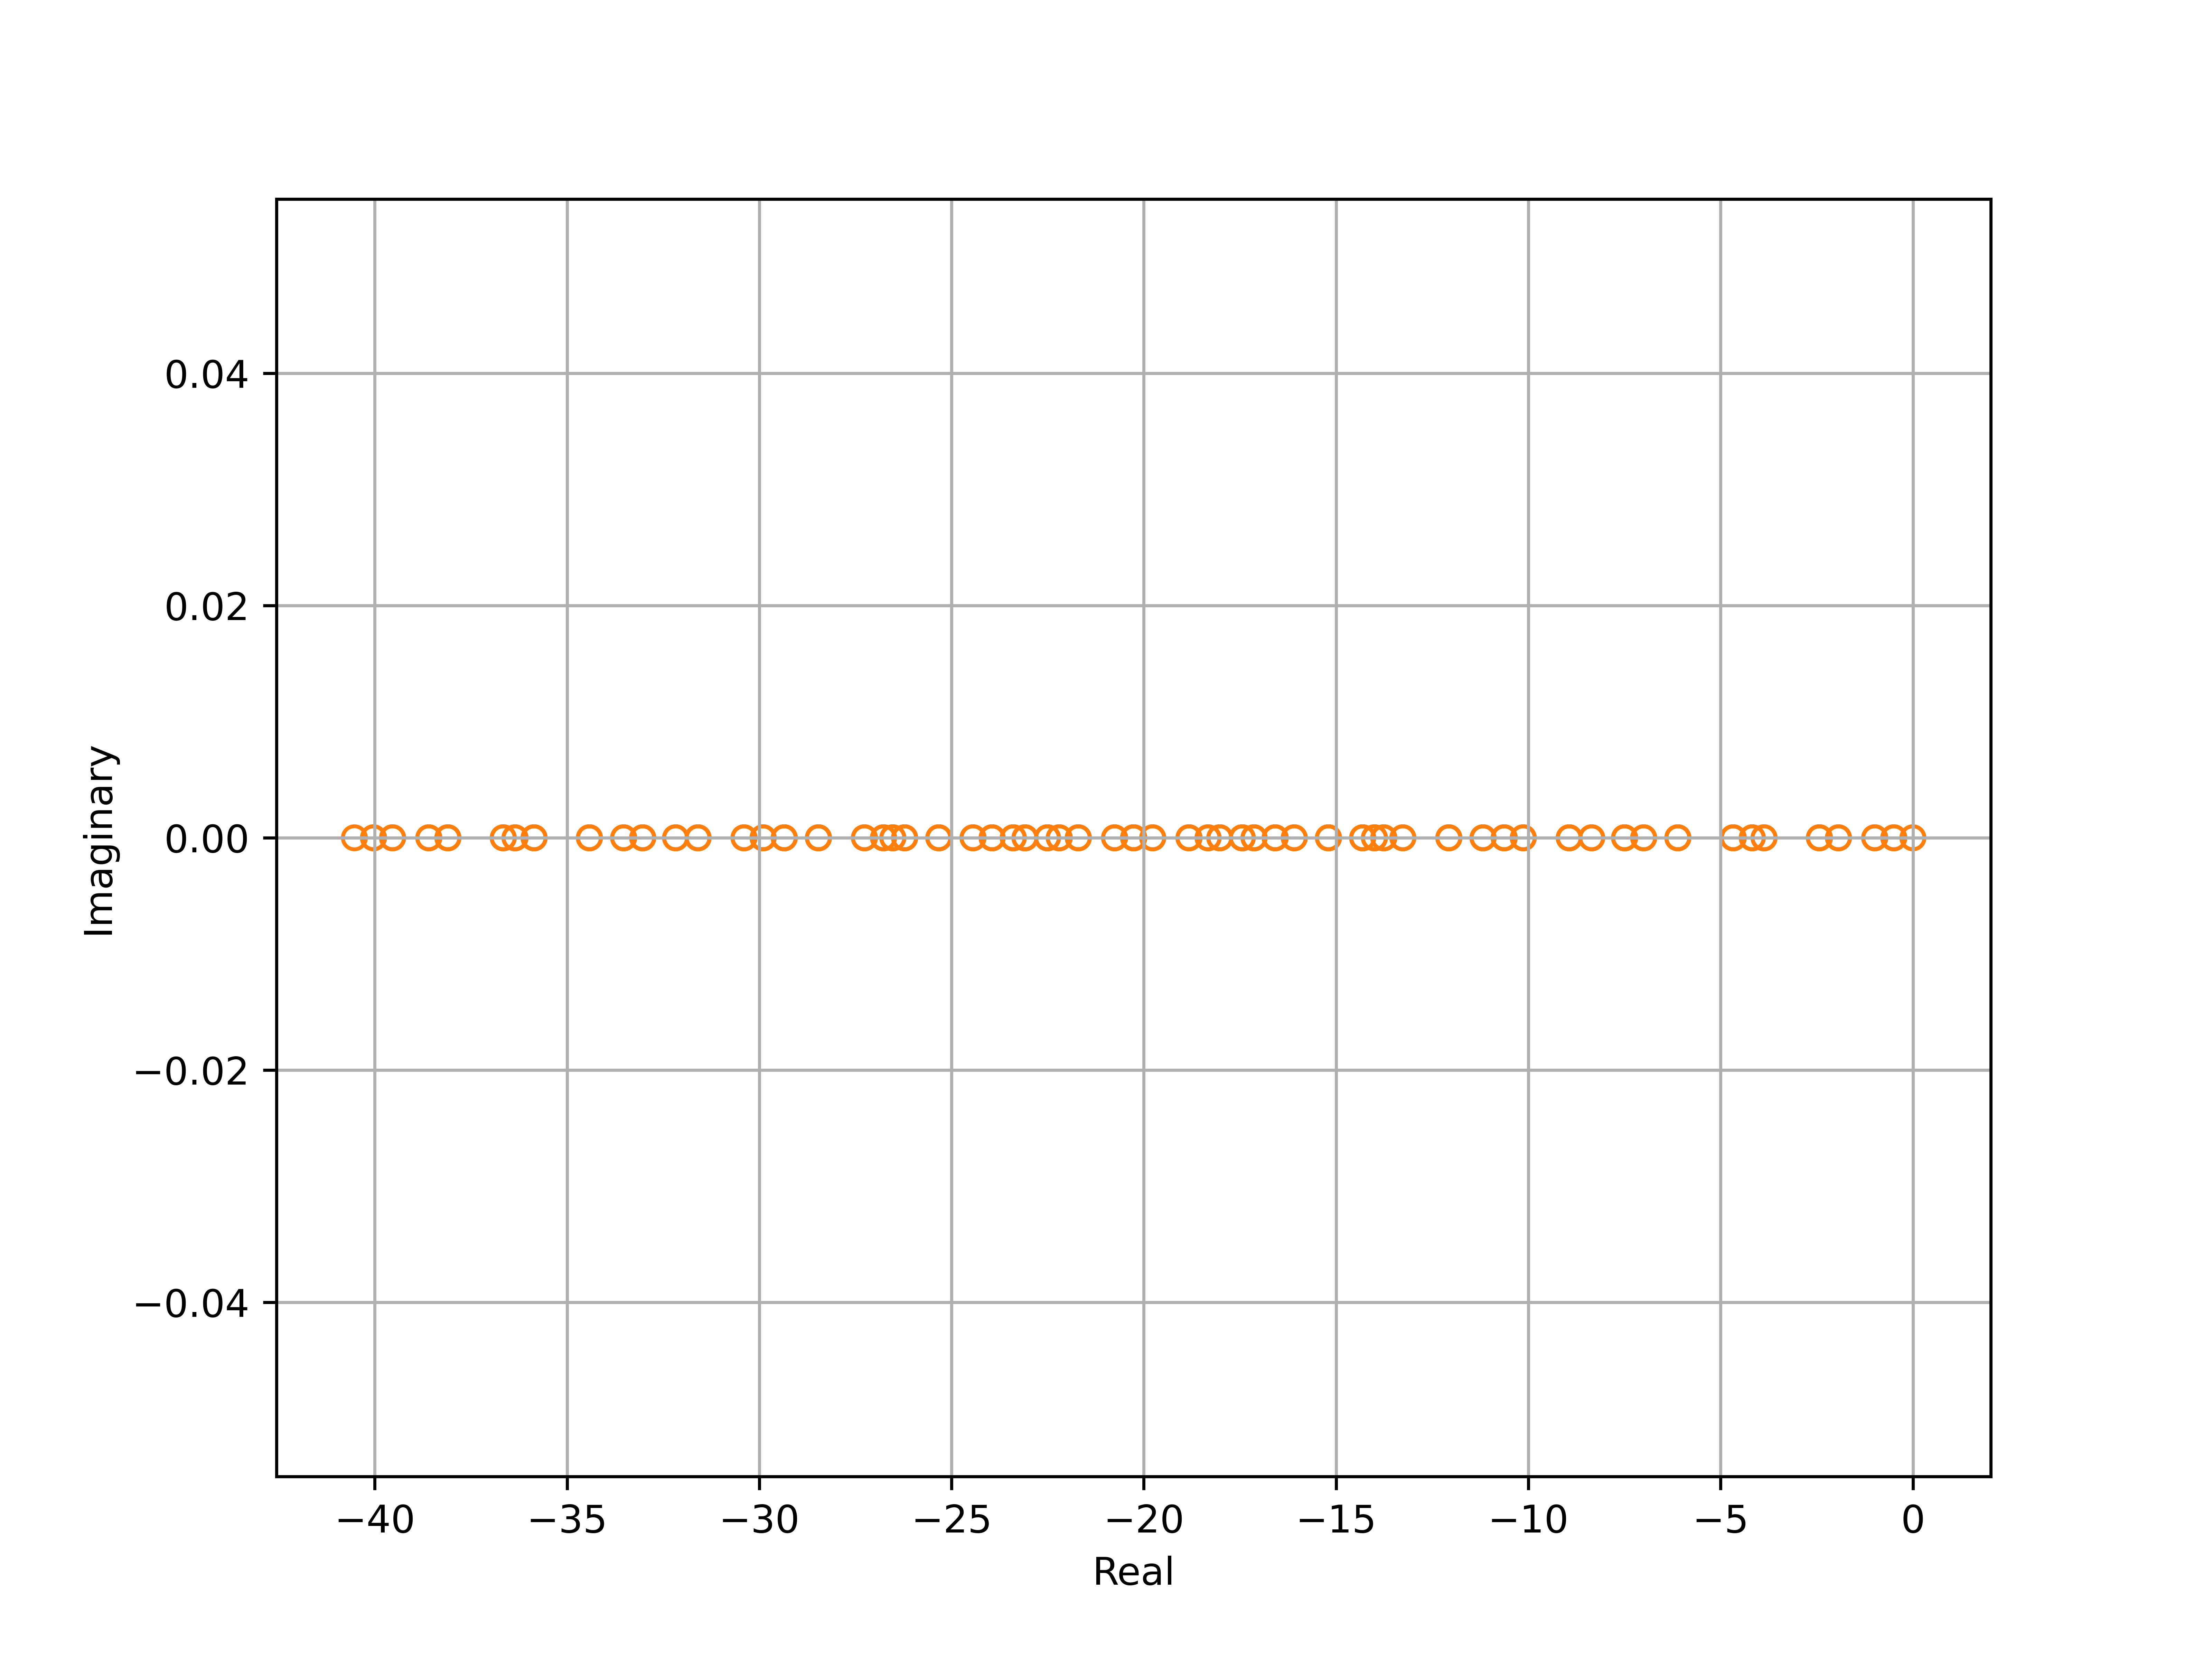
\includegraphics[width=3.9in]{images/chapter-5/progressionProblems/problem1/eigenvaluesDiffusion1-20.png}
    \caption{Eigenvalues for the 400 x 400 case in diffusion problem one}
    \label{fig:eigenvalues_diffusion_one}
\end{figure}

\clearpage

\begin{table}[p]
   \caption{\label{tab:diffusion_problem1_results_krylov} Error and Run Times for Different Krylov Subspace Dimensions}
   \centering
   \begin{tabular}{cllllll}
   \hline
   Solver & M & $l_{\infty}$ Error & $l_{1}$ Error & $l_{2}$ Error & Run time (sec)\\
   \hline
   Pad\'e-method 1 &   5 & 1.74e-05 & 7.05e-06 & 1.12e-02 & 1.13e-02 \\
   - &  10 & 1.74e-05 & 7.05e-06 & 1.12e-02 & 1.47e-02 \\
   - &  25 & 1.74e-05 & 7.05e-06 & 1.12e-02 & 3.31e-02 \\
   - &  50 & 1.74e-05 & 7.05e-06 & 1.12e-02 & 9.27e-02 \\
   - & 100 & 1.74e-05 & 7.05e-06 & 1.12e-02 & 3.33e-01 \\
   - & 150 & 1.74e-05 & 7.05e-06 & 1.12e-02 & 7.30e-01 \\
   - & 200 & 1.74e-05 & 7.05e-06 & 1.12e-02 & 1.33e+00 \\
   \hline
   Pad\'e-method 2 &   5 & 1.74e-05 & 7.05e-06 & 1.12e-02 & 9.15e-03 \\
   - &  10 & 1.74e-05 & 7.05e-06 & 1.12e-02 & 1.18e-02 \\
   - &  25 & 1.74e-05 & 7.05e-06 & 1.12e-02 & 2.96e-02 \\
   - &  50 & 1.74e-05 & 7.05e-06 & 1.12e-02 & 8.95e-02 \\
   - & 100 & 1.74e-05 & 7.05e-06 & 1.12e-02 & 3.28e-01 \\
   - & 150 & 1.74e-05 & 7.05e-06 & 1.12e-02 & 8.20e-01 \\
   - & 200 & 1.74e-05 & 7.05e-06 & 1.12e-02 & 1.55e+00 \\
   \hline
   \end{tabular}
\end{table}


\FloatBarrier
\clearpage

\subsection{Problem 2}
In the second example, a 1D reaction-diffusion problem was modeled. This problem was taken from work performed by Chou et al. (\cite{ching2007}). The partial differential equations (PDEs) are as follows:

\begin{equation}
\setlength{\jot}{15pt}
\begin{split}
    \frac{\partial U}{\partial t} &= d\frac{\partial^{2}U}{\partial x^{2}} - aU + V, \\
    \frac{\partial V}{\partial t} &=
    d\frac{\partial^{2}V}{\partial x^{2}} - bV,
\end{split}
    \label{eq:problem2Eqs}
\end{equation}

\noindent on the domain $x \in [0, \pi/2]$. The system is subject to the following boundary conditions: 

\begin{equation}
    \frac{\partial U}{\partial x}(0,t) = 0, \quad \frac{\partial V}{\partial x}(0,t) = 0, \quad U(\frac{\pi}{2}, t) = 0, \quad V(\frac{\pi}{2}, t)= 0,
\end{equation}

\noindent with the following initial condition:

\begin{equation}
    U(x,0) = 2\cos(x), \quad V(x,0) = (a-b)\cos(x).
\end{equation}

\noindent The exact solution is given by

\begin{equation}
\setlength{\jot}{15pt}
\begin{split}
    U(x,t) = \bigg( e^{-(a+d)t} + e^{-(b+d)t}\bigg)\cos(x), \text{ and} \\
    V(x,t) = (a - b) e^{-(b+d)t}\cos(x).
\end{split}
\end{equation}

The same three test problems that were conducted in the work by Chou et al. (\cite{ching2007}) were also conducted in libowski. These test results correspond to changes in coefficients $[a, b, d]$, which produced a diffusion-dominated system [0.1, 0.01, 1.0], a reaction-dominated system [2.0, 1.0, 0.001], and a stiff reaction system [100, 1.0, 0.001]. Each test case was run with one time step to $t = 1$, so $\Delta t = 1$. The number of cells in the x direction was varied from 10 to 320. Results for the spatial convergence for the Taylor solver for the diffusion-dominated, reaction-dominated and stiff reaction--dominated cases are shown in Tables \ref{tab:diffusion_spatial_convergence_diffusion_dom}, \ref{tab:diffusion_spatial_convergence_reaction_dom}, and \ref{tab:diffusion_spatial_convergence_stiff_reaction_dom}. Each solver produced the same error at up to four decimal places for most of the $n$ values; therefore, only the Taylor results are shown. Full results for these test are shown in Appendix \ref{appen:results} Tables \ref{tab:diffusion_diffusion_dom_problem2_results}, \ref{tab:diffusion_reaction_dom_problem2_results} and \ref{tab:diffusion_stiff_reaction_dom_problem2_results}. As expected, the convergence rate for this problem is second order or better for each of the error metrics.  While there is little difference between the errors from these solvers for this first problem, there is a notable difference in run times for the Pad\'e and Taylor solvers. The E${}_{\infty}$ error and run time for each sub-problem is shown in Figures \ref{fig:problem2_diffusion_dom}, \ref{fig:problem2_reaction_dom} and \ref{fig:problem2_stiff_reaction_dom}. 

Figures \ref{fig:problem2_diffusion_dom}-\ref{fig:problem2_stiff_reaction_dom} show that CRAM is the fastest solver, followed by the parabolic and hyperbolic solvers. Both of the Pad\'e solvers had drastically much longer run times for the diffusion-dominated cases, with Method 2 being the longest. Interestingly, the Taylor solver showed dramatically different run times based on the physical process dominating the problem. In the diffusion-dominated cases, the Taylor solver took the longest, but in the reaction-dominated cases, the run time was on the order of the CRAM, parabolic, and hyperbolic solvers. 

The Krylov subspace approximation was applied to each sub-problem with 1,000 cells in the x direction. The Krylov dimensions were varied from 2 to 100, and the results are shown in Figure \ref{fig:problem2_krylov} . Unlike the previous diffusion example, a much larger Krylov dimension was required to reach a converged error in the diffusion-dominated case. Each solver showed the same error behavior, but with slightly different converged errors due to numerical accuracy in the algorithms. Each solver also showed similar behavior, with run time scaling as a function of the Krylov dimension; however, each axis was scaled differently. Applying the Krylov subspace to each Pad\'e solver reduced the many orders of magnitude, but it failed to reduce the run time of the Taylor solver to the same order in the diffusion-dominated case. For each of the reaction-dominated cases, the Krylov subspace dimension required to reach a converged solution is much smaller than the diffuion-dominated case. 

\clearpage

\begin{table}[h]
   \caption{\label{tab:diffusion_spatial_convergence_diffusion_dom} Convergence Rate for Diffusion-Dominated Problem Using Absolute Error}
   \centering
   \begin{tabular}{lllllll}
   \hline
    n & E${}_{\infty}$ Rate & E${}_{1}$ Rate & E${}_{2}$ Rate & E${}_{\infty}$ Error & E${}_{1}$ Error & E${}_{2}$ Error\\
   \hline
    20 & 2.00 & 2.00 & 2.50 & 1.87e-04 & 1.19e-04 & 2.97e-05 \\ 
    40 & 2.00 & 2.00 & 2.50 & 4.69e-05 & 2.99e-05 & 5.24e-06 \\ 
    80 & 2.00 & 2.00 & 2.50 & 1.17e-05 & 7.46e-06 & 9.27e-07 \\ 
   160 & 2.00 & 2.00 & 2.50 & 2.93e-06 & 1.87e-06 & 1.64e-07 \\ 
   320 & 2.00 & 2.00 & 2.50 & 7.33e-07 & 4.66e-07 & 2.90e-08 \\ 
   \hline
   \end{tabular}
\end{table}

\begin{table}[h]
   \caption{\label{tab:diffusion_spatial_convergence_reaction_dom} Convergence Rate for Reaction-Dominated Problem Using Absolute Error}
   \centering
   \begin{tabular}{lllllll}
   \hline
    n & E${}_{\infty}$ Rate & E${}_{1}$ Rate & E${}_{2}$ Rate & E${}_{\infty}$ Error & E${}_{1}$ Error & E${}_{2}$ Error\\
   \hline
    20 & 2.00 & 2.00 & 2.50 & 2.23e-04 & 1.42e-04 & 3.53e-05 \\  
    40 & 2.00 & 2.00 & 2.50 & 5.58e-05 & 3.55e-05 & 6.24e-06 \\  
    80 & 2.00 & 2.00 & 2.50 & 1.40e-05 & 8.88e-06 & 1.10e-06 \\  
   160 & 2.00 & 2.00 & 2.50 & 3.49e-06 & 2.22e-06 & 1.95e-07 \\  
   320 & 2.00 & 2.00 & 2.50 & 8.72e-07 & 5.55e-07 & 3.45e-08 \\  
   \hline
   \end{tabular}
\end{table}

\begin{table}[h]
   \caption{\label{tab:diffusion_spatial_convergence_stiff_reaction_dom} Convergence Rate for Stiff Reaction--Dominated Problem Using Absolute Error}
   \centering
   \begin{tabular}{lllllll}
   \hline
    n & E${}_{\infty}$ Rate & E${}_{1}$ Rate & E${}_{2}$ Rate & E${}_{\infty}$ Error & E${}_{1}$ Error & E${}_{2}$ Error\\
   \hline
    20 & 2.00 & 2.00 & 2.50 & 9.42e-03 & 6.00e-03 & 1.49e-03 \\ 
    40 & 2.00 & 2.00 & 2.50 & 2.36e-03 & 1.50e-03 & 2.63e-04 \\ 
    80 & 2.00 & 2.00 & 2.50 & 5.89e-04 & 3.75e-04 & 4.66e-05 \\ 
   160 & 2.00 & 2.00 & 2.50 & 1.47e-04 & 9.38e-05 & 8.23e-06 \\ 
   320 & 2.00 & 2.00 & 2.50 & 3.68e-05 & 2.34e-05 & 1.46e-06 \\ 
   \hline
   \end{tabular}
\end{table}

\clearpage

\begin{figure}[p]
    \centering
    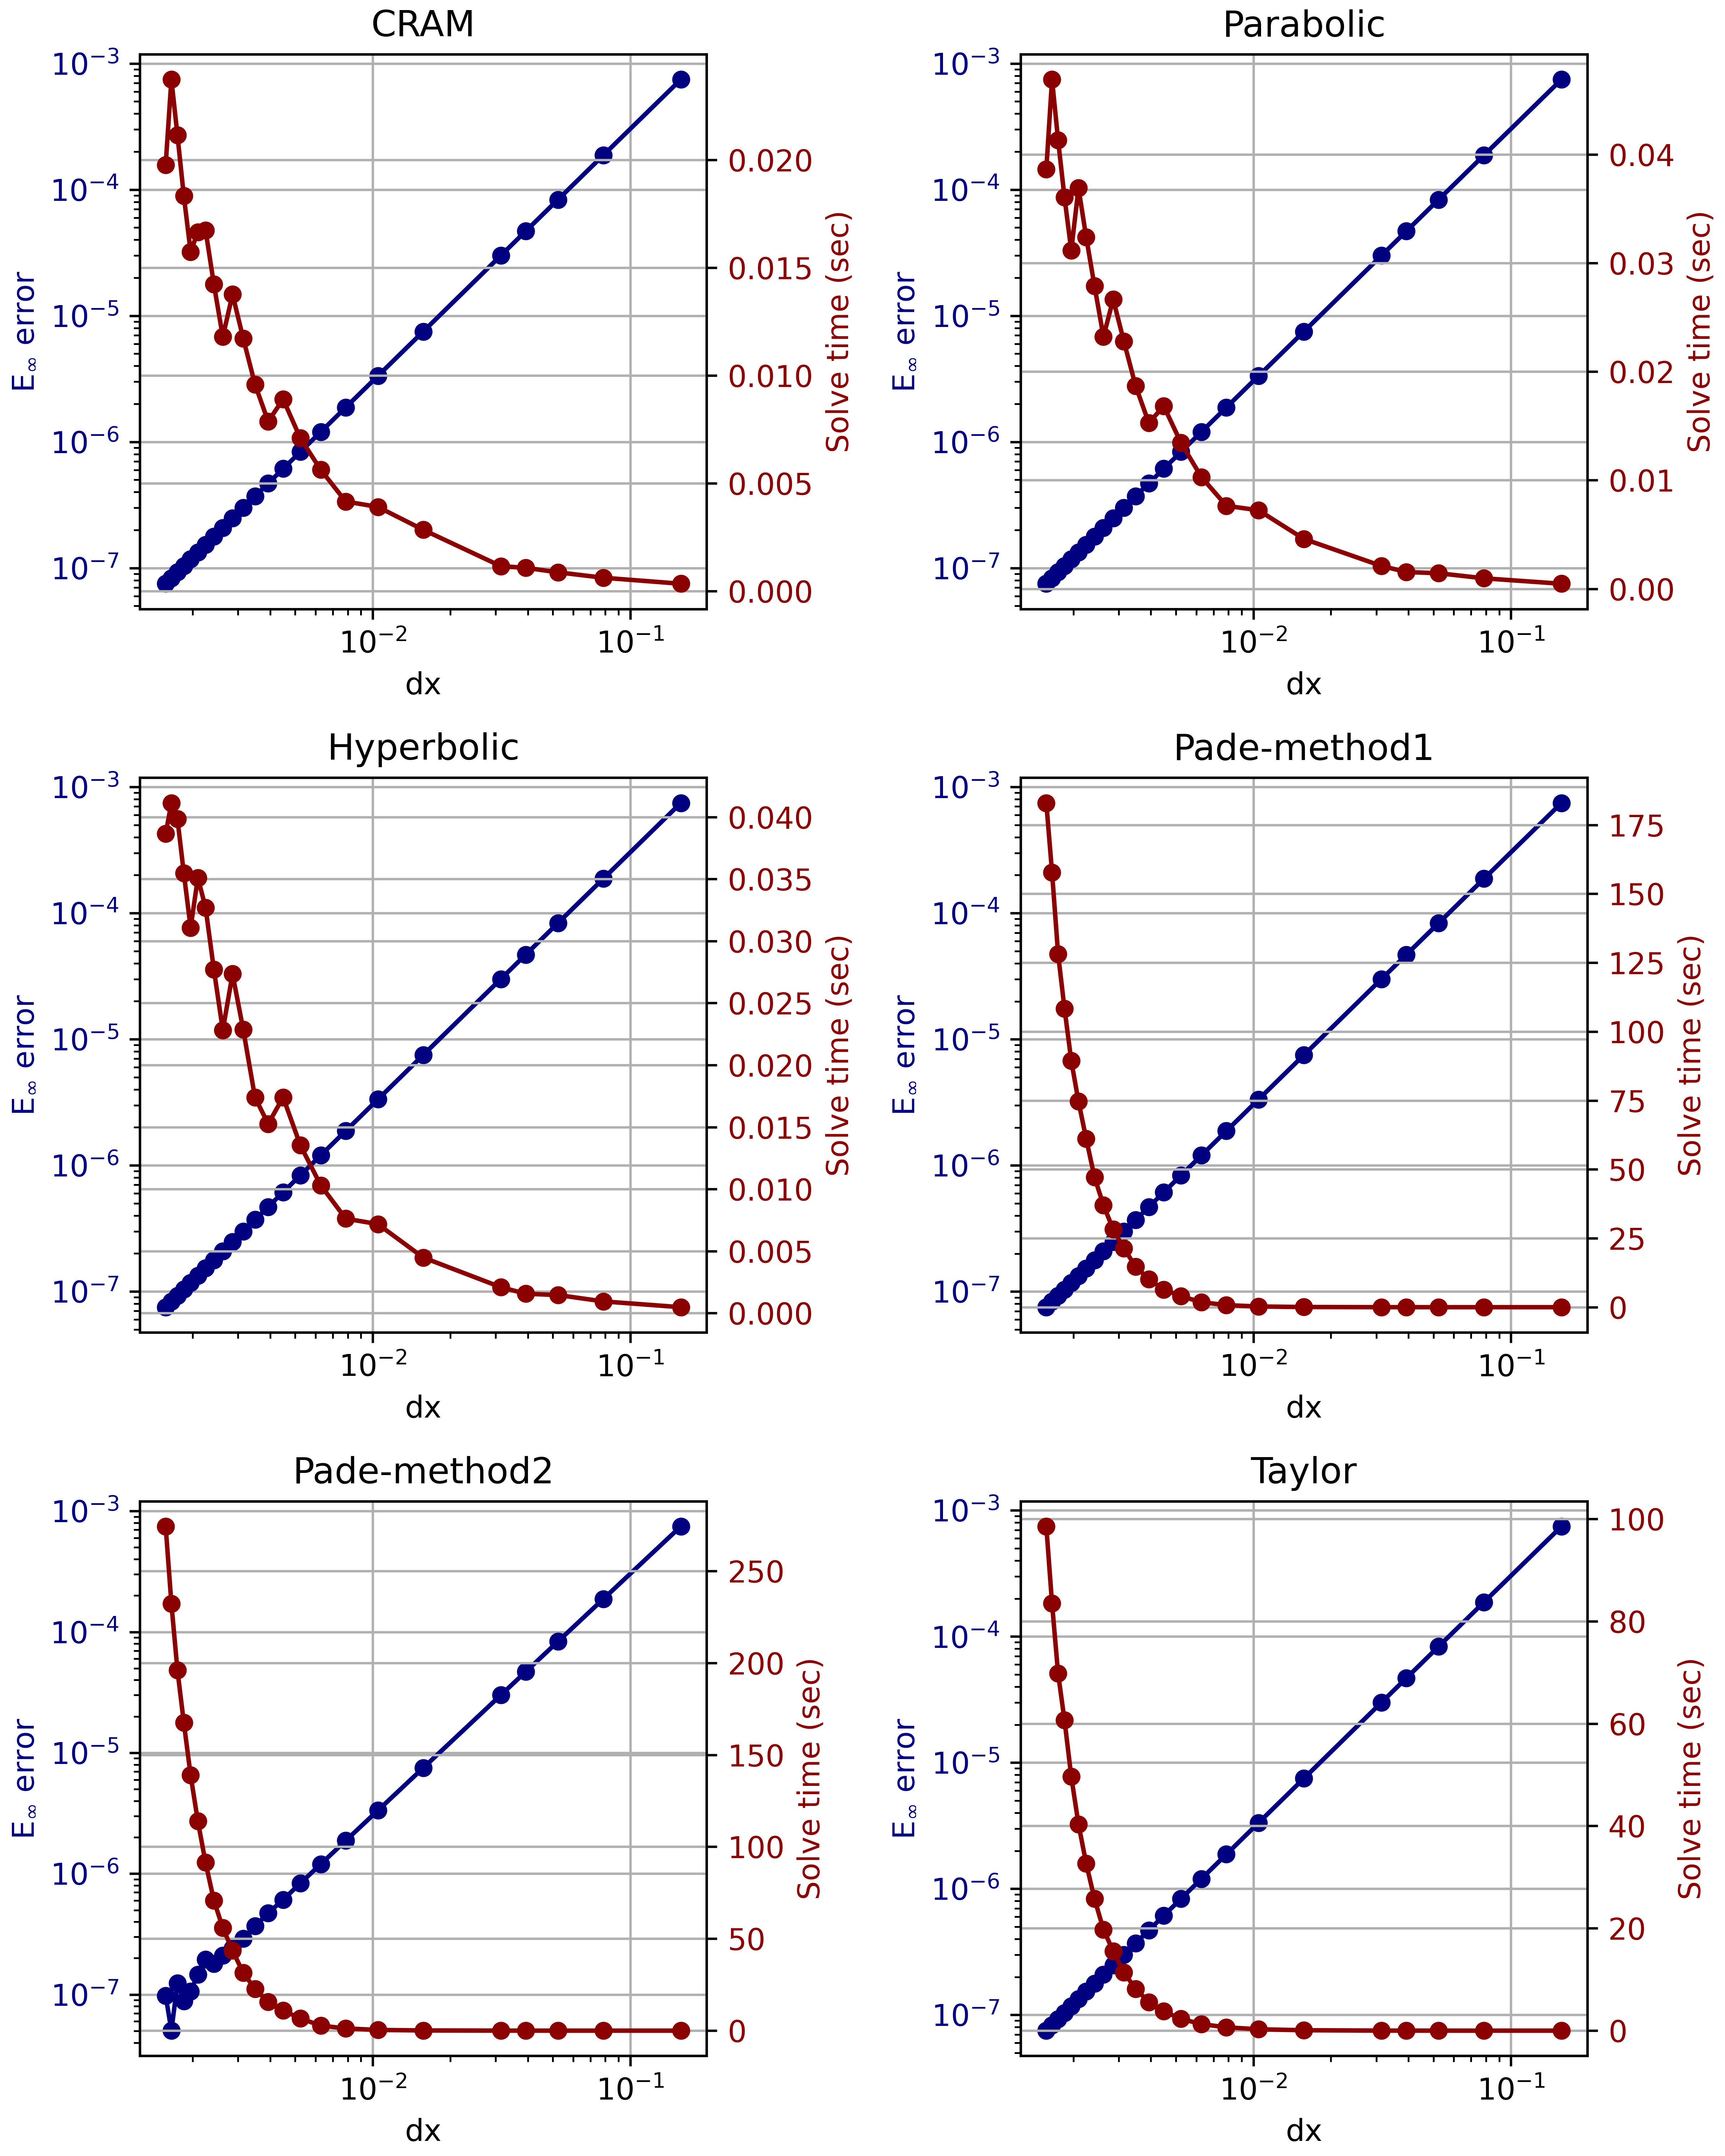
\includegraphics[width=5.0in]{images/chapter-5/progressionProblems/problem2/problem2a.png}
    \caption{Results for the diffusion-dominated case}
    \label{fig:problem2_diffusion_dom}
\end{figure}

\clearpage

\begin{figure}[p]
    \centering
    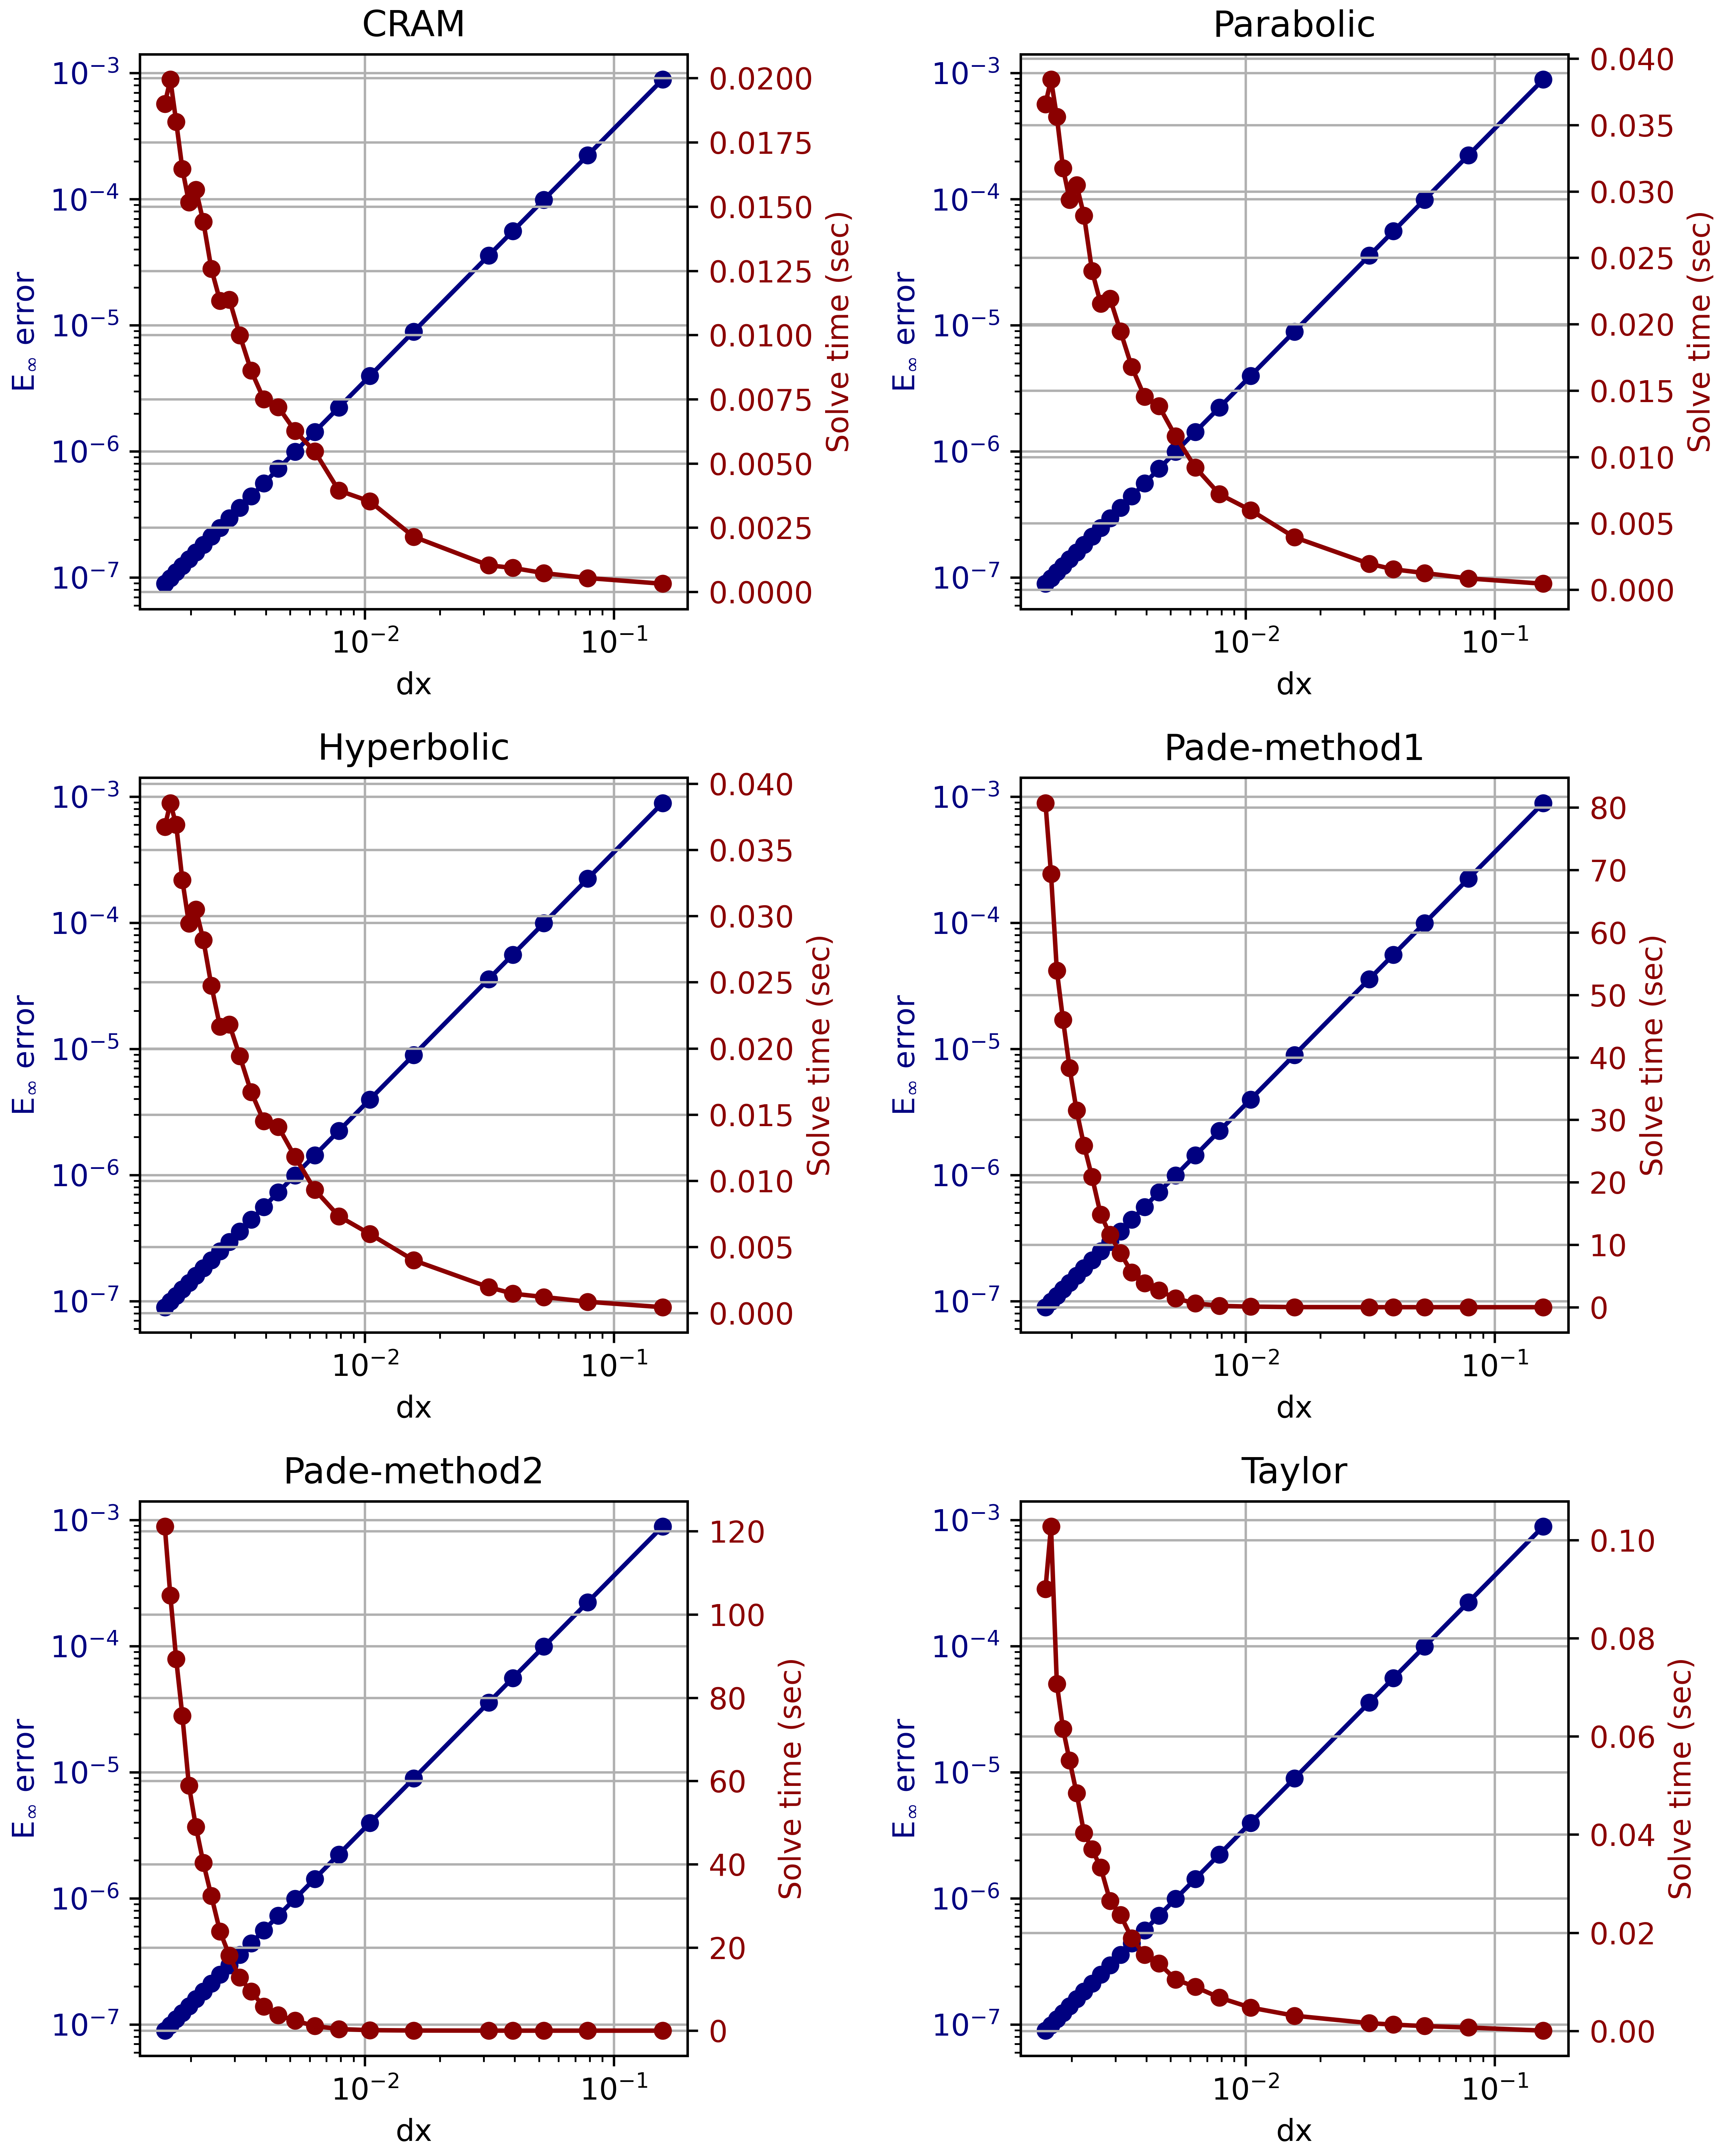
\includegraphics[width=5.0in]{images/chapter-5/progressionProblems/problem2/problem2b.png}
    \caption{Results for the reaction-dominated case}
    \label{fig:problem2_reaction_dom}
\end{figure}

\clearpage

\begin{figure}[p]
    \centering
    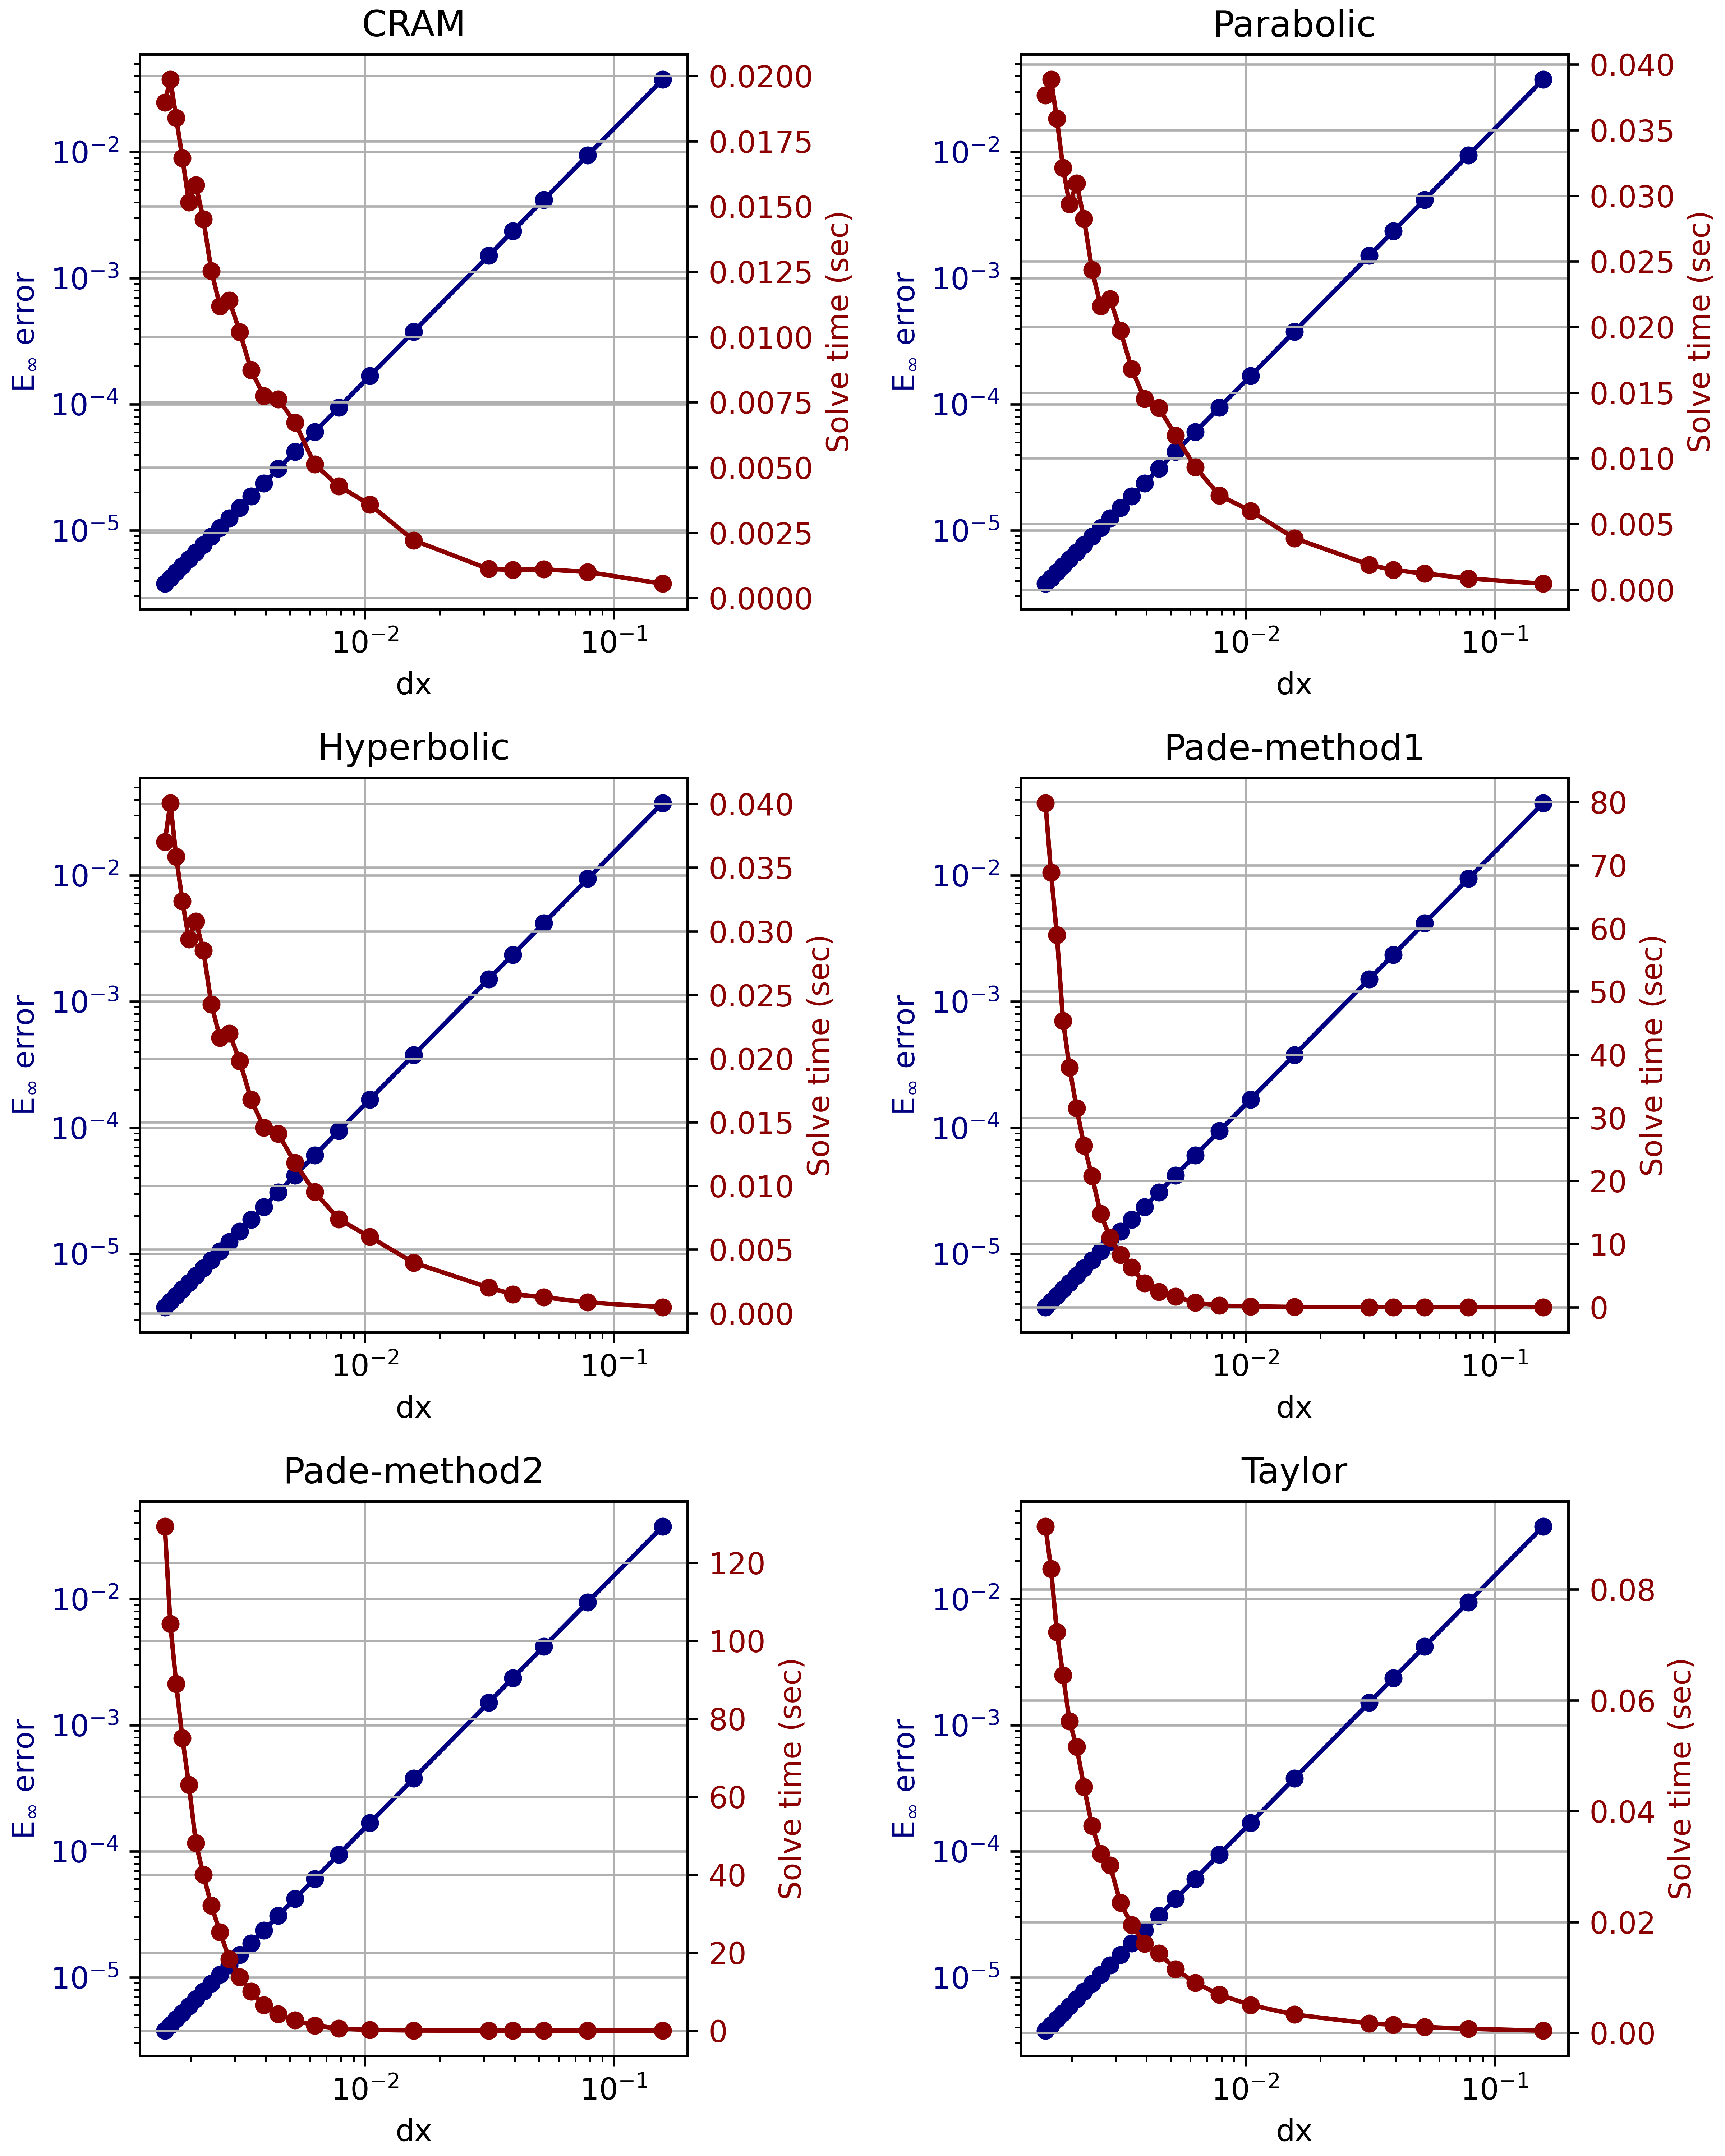
\includegraphics[width=5.0in]{images/chapter-5/progressionProblems/problem2/problem2c.png}
    \caption{Results for the stiff reaction-dominated case}
    \label{fig:problem2_stiff_reaction_dom}
\end{figure}

\clearpage

\begin{sidewaysfigure}[htbp]
    \centering
    \includegraphics[width=8in]{images/chapter-5/progressionProblems/problem2/krylovProblem2.png}
    \caption{Results for the Krylov subspace approximation for each sub-problem}
    \label{fig:problem2_krylov}
\end{sidewaysfigure}

\clearpage

\subsection{Problem 3}

Convection was tested using PDE of the form

\begin{equation}
    \frac{\partial U}{\partial t} = -v\frac{\partial U}{\partial x},
    \label{eq:convection_PDE}
\end{equation}

\noindent where $v$ is velocity. Equation (\ref{eq:convection_PDE}) was applied to a system on the domain $x \in [0, 100]$, $t \in [0, 20]$ subject to the following boundary conditions:

\begin{equation}
    U(0,t) = 1.0, \quad\frac{\partial U}{\partial x}(100, t) = 0.0,
\end{equation}

\noindent and the initial condition:

\begin{equation}
    U(x,0) = 0.0.
\end{equation}

What is most important about this problem is that it exposes an instability with Cauchy solvers which seems to be specific to this problem. This is something that is not seen with the series solvers such as Pad\'e or Taylor. First, results for the first order upwind differencing scheme are shown in Figure \ref{fig:first_order_results}  for a first-order backward differencing formula (BDF1) and the ETD scheme using the series matrix exponential solvers. While only the Taylor solver is shown, results for the Pad\'e solvers are the same. Figure \ref{fig:first_order_results} shows the typical reduction in numerical diffusion with decreasing dx. In figure \ref{fig:first_order_results} we see that as the time step size decreases for the explicit BDF1 solver it approaches the accuracy of the ETD method with a single time step. 

The instability seen with Cauchy solvers is shown in figure \ref{fig:first_order_results_cauchy_instability} for a zoomed in and zoomed out view of each solution. In figure \ref{fig:first_order_results_cauchy_instability} it is seen that for dx values 0.5 and 0.4, the solution blows up and oscillates. What is important to note that even know the solution for dx = 1.0 is stable it does contain small negative values as it approaches zero. The matrix exponential is the analytical solution to the ODE system and should not show any instability, so the instability shown here is due to the numerical computation of the exponential itself. To combat this instability the order of the method can be increased, this is seen in figure \ref{fig:first_order_results_cauchy_instability_different_orders}. Figure \ref{fig:first_order_results_cauchy_instability_different_orders} shows the Hyperbolic and Parabolic solvers at different order of N. As the order in increased, the solution becomes more stable.  Another method to increase the stability of the solution is to compute the solution with multiple steps and not just at the final time step. This is equivalent to using the substep method for the Cauchy solvers. Figure \ref{fig:first_order_results_cauchy_instability_different_time_steps} shows results for each of the Cauchy solver for different time step sizes. Even with large time step sizes the solution becomes stable.   \textcolor{red}{Discuss accuracy related to the Jordan canonical form.}

To illustrate the enhanced accuracy of TVD non-linear flux limiters, the same problem is conducted with a variety of limiter functions. This method works to approximate the convection term to at most second order in the case of smooth solutions and reduce numerical diffusion seen in the first order case. Figure \ref{fig:fluxlimiters_problem3} shows results from each of the flux limiter functions in libowski using the Taylor solver. Each of the flux limiter functions reduces the numerical diffusion, seen in the first order upwind case with superbee being the best. While the TVD scheme is designed to remove unphysical oscillations seen in higher order convection schemes, these oscillations are present because of the explicit implementation. Figure \ref{fig:fluxlimiters_instability_problem3} shows these oscillations for six flux limiter functions. This behavior is only present when large time step sizes are used. For some time integration methods, explicit schemes are known to be unstable if large time step sizes are used. In this case the second order correction being calculated from the previous time step causes the solution to become unstable if large enough time steps are taken. This same behavior is seen in all the ETD matrix exponential solvers. 

\clearpage

\begin{figure}[p]
    \centering
    \includegraphics[width=6in]{images/chapter-5/progressionProblems/problem3/problem3FirstOrder.png}
    \caption{First-order upwind differencing with series solvers and BDF1}
    \label{fig:first_order_results}
\end{figure}

\clearpage

\begin{figure}[p]
    \centering
    \includegraphics[width=6.0in]{images/chapter-5/progressionProblems/problem3/problem3FirstOrderCauchyInstability.png}
    \caption{First-order upwind differencing instability for Cauchy solvers}
    \label{fig:first_order_results_cauchy_instability}
\end{figure}

\clearpage

\begin{figure}[p]
    \centering
    \includegraphics[width=5.0in]{images/chapter-5/progressionProblems/problem3/problem3FirstOrderCauchyInstabilityDifferentOrders.png}
    \caption{First-order upwind differencing instability for Cauchy solvers at different orders}
    \label{fig:first_order_results_cauchy_instability_different_orders}
\end{figure}

\clearpage

\begin{figure}[p]
    \centering
    \includegraphics[width=6in]{images/chapter-5/progressionProblems/problem3/problem3FirstOrderCauchyInstabilityDifferentTimeSteps.png}
    \caption{First-order upwind differencing instability for Cauchy solvers at different time step sizes}
    \label{fig:first_order_results_cauchy_instability_different_time_steps}
\end{figure}

\clearpage

\begin{figure}[p]
    \centering
    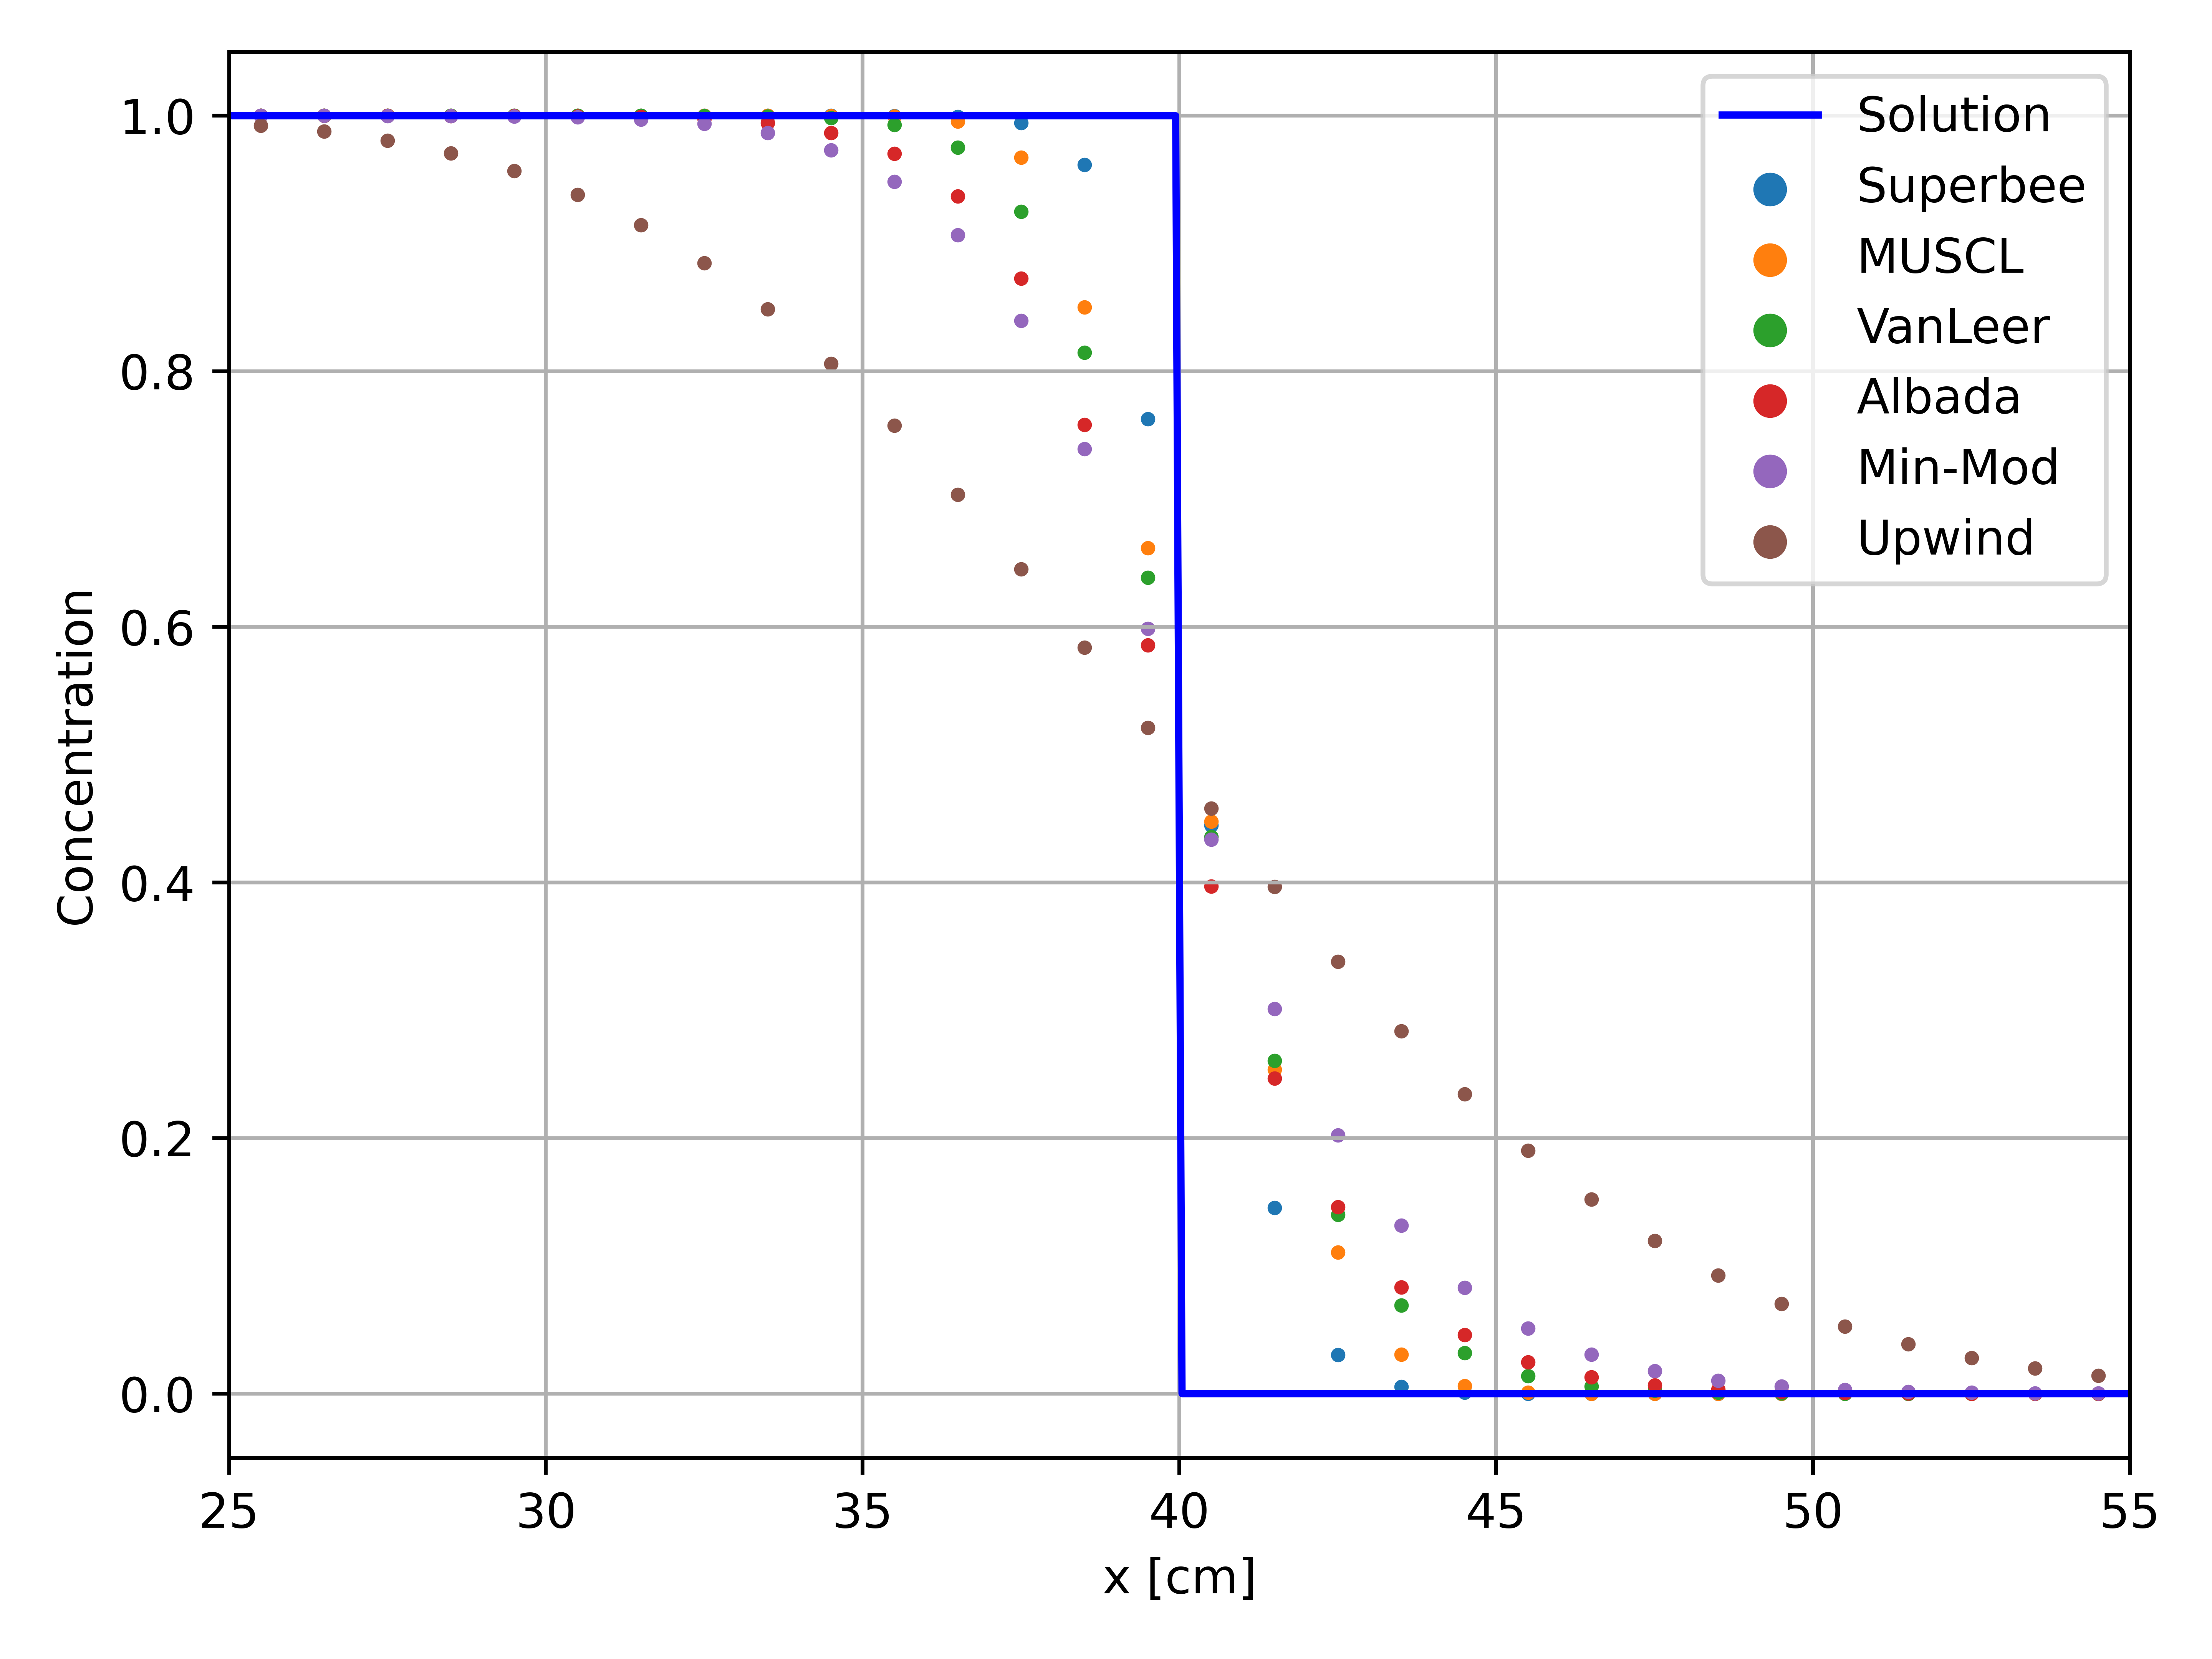
\includegraphics[width=5in]{images/chapter-5/progressionProblems/problem3/problem3FluxLimiters.png}
    \caption{Flux limiter function applied to problem three, dt = 0.1, dx = 0.2}
    \label{fig:fluxlimiters_problem3}
\end{figure}

\clearpage

\begin{figure}[p]
    \centering
    \includegraphics[width=6in]{images/chapter-5/progressionProblems/problem3/problem3SecondOrderFluxLimiterFunctionInstability.png}
    \caption{Instability of flux limiter functions with the Taylor solver}
    \label{fig:fluxlimiters_instability_problem3}
\end{figure}

\clearpage

\subsection{Problem 4}

The same PDE that was shown in the previous problem is tested again:

\begin{equation}
    \frac{\partial U}{\partial t} = -v\frac{\partial U}{\partial x},
    \label{eq:convection_PDE}
\end{equation}

\noindent on the domain $x \in [0, 100]$, $t \in [0, 5]$ subject to periodic boundary conditions:

\begin{equation}
    U(0,t) = U(100, t),
\end{equation}

\noindent and the initial condition:

\begin{equation}
    U(x,0) = \exp\bigg\{-\bigg(\frac{(x-30)}{10}\bigg)^{2}\bigg\}.
\end{equation}

\noindent with the following solution:

\begin{equation}
	U(x,t)_ = \exp\bigg\{-\bigg(\frac{(x-vt-30)}{10}\bigg)^{2}\bigg\}.
\end{equation}

Figure \ref{fig:problem4_l1error_spatial_results} shows E${}_{1}$ error behavior as a function of spatial discretization at various time step sizes. Figure \ref{fig:problem4_l1error_time_results} shows the same error behavior as a function of temporal discretization at various number of spatial cells. Figure \ref{fig:problem4_l1error_spatial_results} shows that as the number of time steps take is increased the higher order flux limiters begin to show a linear relationship with spatial discretization. This can be readily seen with the number of steps greater than 40. The upwind limiter is unaffected by decreasing the time step size, which is to be expected. This is because increasing the number of times steps do nothing to increase its accuracy. Figure \ref{fig:problem4_l1error_time_results} shows that increasing the number of time steps has little to no affect on the error for large spatial discretization. As the number of cells increases, decreasing the time step size has a greater affect on reducing the error. This figure also reiterates the fact that the first order upwind error is not affected by increasing the number of time steps taken. Results for the E${}_{\infty}$ and E${}_{2}$ errors are shown in Appendix \ref{appen:results} figures \ref{fig:problem4_linferror_spatial_results}, \ref{fig:problem4_linferror_time_results}, \ref{fig:problem4_l2error_spatial_results} and \ref{fig:problem4_l2error_time_results}. Figure \ref{fig:problem4_linferror_spatial_results} shows a similar trend with spatial refinement using the E${}_{\infty}$ error to the E${}_{1}$ error however, the error function in figure \ref{fig:problem4_linferror_spatial_results} does not maintain the same linear rate. This relation is further represented in Figure \ref{fig:problem4_linferror_time_results} which shows the error with temporal refinement. For large spatial refinement, the error remains constant. For smaller refinement, the error takes a dip then increases. The E${}_{2}$ error shown in figures \ref{fig:problem4_l2error_spatial_results} and \ref{fig:problem4_l2error_time_results} shows a trend resembling the E${}_{1}$ error, in which the error convergence rate remains semi linear as a function of spatial discretization for most flux limiters with larger number of time steps. 

Figure \ref{fig:problem4_l1error_fluxlimiter_convergence_rate} shows convergence rates for each of the higher order flux limiter functions as a function of space and time using the E${}_{1}$ error. Each flux limiter shows a dark zone (representing low convergence rate) with high spatial discretization and low temporal discretization. At 320 spatial cells, the convergence rate of each flux limiter increases until reaching an apex at 40 time steps, then slightly decreases to a constant-ish value. At low spatial resolution, increases the number of time steps taken does not have a large affect on changing the convergence rate. Results for the E${}_{\infty}$ and E${}_{2}$ error metrics are shown in Appendix \ref{appen:results} figures \ref{fig:problem4_linferror_fluxlimiter_convergence_rate} and \ref{fig:problem4_l2error_fluxlimiter_convergence_rate}. Behavior of the E${}_{2}$ error shows similar trends to $l_{1}$, low convergence rates for high spatial resolution and low temporal, with most limiters showing peak convergence with 8 or 40 time steps and 320 cells. Convergence rates for E${}_{\infty}$ error are shown in figure \ref{fig:problem4_linferror_fluxlimiter_convergence_rate}. These results show convergence rates which are slightly worse than the other two errors. The peak convergence rate for most flux limiters has also shifted from 320 cells and 40 time steps to 320 cells and 8 time steps. All limiter functions also show a general trend of having larger convergence rates at lower spatial resolution. 

Figure \ref{fig:problem4_runtimes} shows the average run time results for each of the solvers. Each flux limiter function call requires the same time meaning that small run time differences for each solve is due to the computers computation. For the small cases, the Taylor and Pad\'e solvers out perform the Cauchy solvers. As the number of cells increase, the Pad\'e solver run times begin to approach values greater than the Cauchy solvers. Hyperbolic and Parabolic remain about the same as seen before, with CRAM being the lowest of the three. The Taylor solver remains the lowest for all problem sizes. 

Unlike the previous example, no instabilities were noticed while conducting the numerical test. Even at large spatial resolutions and small time steps, the flux limiter functions remained stable. Each of the Cauchy solvers also remained stable during testing. While only results for the Taylor solver are shown, all other solvers show the same errors and convergence rates.

\clearpage

\begin{figure}[p]
    \centering
    \includegraphics[width=6in]{images/chapter-5/progressionProblems/problem4/problem4E1ErrorWithSpace.png}
    \caption{Problem 4 absolute E${}_{1}$ error with spatial discretization at various time steps }
    \label{fig:problem4_l1error_spatial_results}
\end{figure}

\clearpage

\begin{figure}[p]
    \centering
    \includegraphics[width=6in]{images/chapter-5/progressionProblems/problem4/problem4E1ErrorWithTime.png}
    \caption{Problem 4 absolute E${}_{1}$ error with temporal discretization at various number of spatial cells}
    \label{fig:problem4_l1error_time_results}
\end{figure}

\clearpage

\begin{figure}[p]
    \centering
    \includegraphics[width=6in]{images/chapter-5/progressionProblems/problem4/problem4E1FluxLimiterConvergenceRate.png}
    \caption{Problem 4 flux limiter E${}_{1}$ spatial convergence rate using absolute error}
    \label{fig:problem4_l1error_fluxlimiter_convergence_rate}
\end{figure}

\clearpage

\begin{figure}[p]
    \centering
    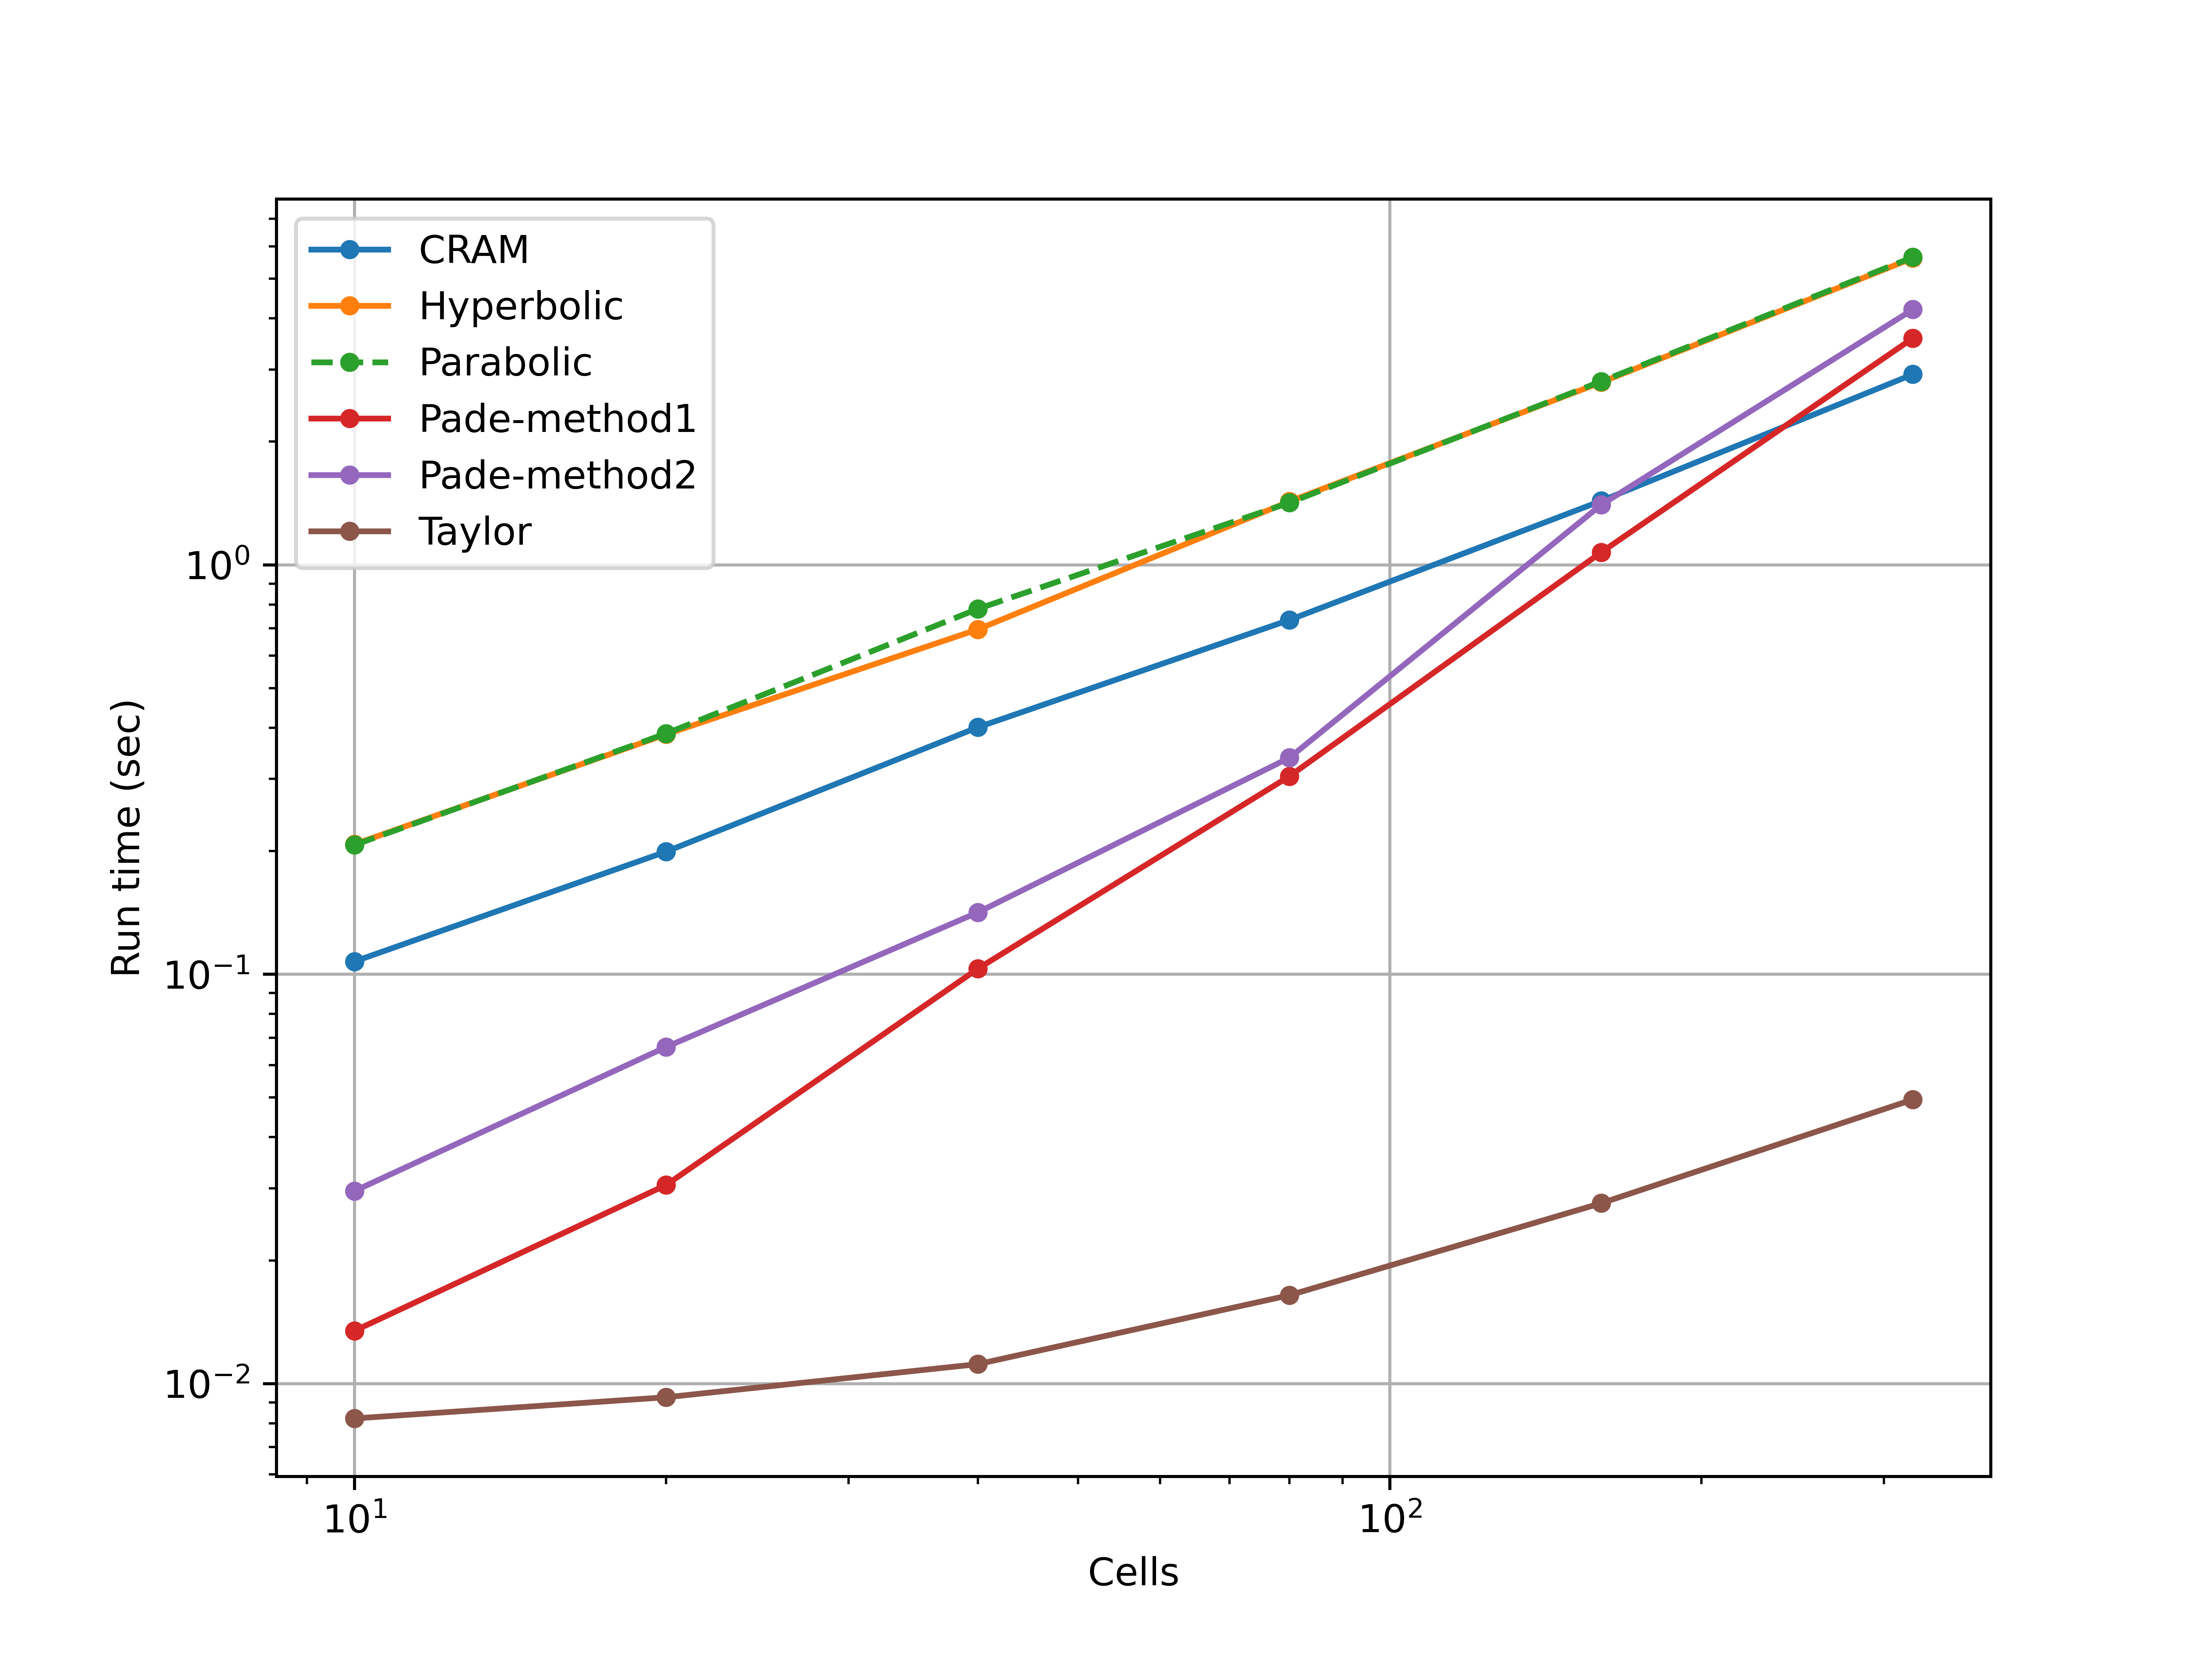
\includegraphics[width=6in]{images/chapter-5/progressionProblems/problem4/problem4Runtimes.png}
    \caption{Problem 4 average run times for each solver, dt = 0.01}
    \label{fig:problem4_runtimes}
\end{figure}

\clearpage

\subsection{Problem 5}
This problem consist on a convection-reaction problem with a single species represented by:

\begin{equation}
    \frac{\partial C}{\partial t} = -v\frac{\partial C}{\partial x} - \lambda C,
\end{equation}

\noindent on the domain $x \in [0,100]$, $t \in [0,20]$ where $v = 2$ and $\lambda = 0.01$. Subject to the following conditions:

\begin{equation}
    C(x, 0) = 1000, \quad C(0,t) = 1000, \quad \frac{dC}{dx}(100, t) = 0.
\end{equation}

\noindent This leads to the analytic solution:

\begin{equation}
C (x,t) = \begin{cases}
  C (x, 0) e^{-\frac{x \lambda _i}{v}}\ , & x < vt \\
  C (x, 0) e^{-t \lambda _i}\ , & x \ge vt
\end{cases}
\end{equation}

This problem is a 1D convection driven flow where the species decays at a constant rate. The solution to this leads to a function that is not smooth, causing the higher order flux limiter functions to reduced to first order accuracy. Figures \ref{fig:problem5_l1error_spatial_results} and \ref{fig:problem5_l1error_time_results} show results for each of the flux limiter functions for the E${}_{1}$ relative error for spatial and temporal discretization. Starting with figure \ref{fig:problem5_l1error_spatial_results}, each of the flux limiters show about the same convergence rate at the first order upwind function. This agrees with the previous statement about TVD schemes reducing to first order convergence rates for non smooth solutions. While the TVD schemes do not have second order convergence rates, they do increase the accuracy of the solution when compared to first order upwind. This is most prevalent with the Albada limiter, which does show are higher convergence rate with large number of cells and time steps. This limiter also maintains the lowest error for all test shown if figures \ref{fig:problem5_l1error_spatial_results} and \ref{fig:problem5_l1error_time_results}. Albada also benefits the most from increasing the number of time steps, this is easly seen in figure \ref{fig:problem5_l1error_time_results}. Figure \ref{fig:problem5_l1error_time_results} also shows that each of the other flux limiter functions are not greatly affected by increasing the number of time steps. For smaller spatial discretizations, increasing the number of time steps does slightly increase the accuracy of the other TVD schemes. Results using the E${}_{\infty}$ and E${}_{2}$ errors are found in Appendix \ref{appen:results} figures \ref{fig:problem5_linferror_spatial_results}, \ref{fig:problem5_linferror_time_results}, \ref{fig:problem5_l2error_spatial_results} and \ref{fig:problem5_l2error_time_results}. Figure \ref{fig:problem5_linferror_spatial_results} shows that the E${}_{\infty}$ error behaves a little worse than E${}_{1}$, showing different flux limiters achieve minimal error at higher spatial resolution. While Albada is still one of the best, it does not have the lowest error for higher spatial and temporal resolutions. The E${}_{2}$ error, shown in figure \ref{fig:problem5_l2error_spatial_results}, shows the same behavior as E${}_{1}$. The Albada limiter performs the best and is affected the most by increasing the number of time steps.  

Figure \ref{fig:problem5_l1error_fluxlimiter_convergence_rate} shows convergence rates as a function of time and space. Unlike problem 4, which showed minimal convergence rate in the bottom left corner, these results show the minimal to be in the top left. This corresponds to low spatial and temporal resolution. For each limiter function, the convergence rate is increased by increasing the number of time steps taken. Just as with figures \ref{fig:problem5_l1error_spatial_results} and \ref{fig:problem5_l1error_time_results}, figure \ref{fig:problem5_l1error_fluxlimiter_convergence_rate} shows the the Albada limiter has the highest convergence rate, reaching a sweet spot at 80 cells and 400 time steps. Figures \ref{fig:problem5_linferror_fluxlimiter_convergence_rate} and \ref{fig:problem5_l2error_fluxlimiter_convergence_rate} shows convergence rates for E${}_{\infty}$ and E${}_{2}$ errors. The $l_{\infty}$ error shows high convergence rates for for low cells and high time steps for all but the Albada and Min-Mod limiters. The E${}_{2}$ error shows high convergence rates for high time steps, generally reaching a plateau as the number of cells in increased.

Figure \ref{fig:problem5_l1error_coefficient_changes} shows how the problem behaves as a function of $v$ and $\lambda$. These coefficients are changed to induce and reaction or velocity dominated system. In a reaction dominated system, all of the flux limiter functions converge to a single point. This is because the accuracy of the solution is dominated by the integration of the reaction rate of the time interval. As the velocity is increased, the flux limiters begin to diverge to difference accuracy's. The Albada limiter diverges the most, decreasing the error 2 orders of magnitude below all the others. What is also interesting is that the error follows a hump shape, increasing up until it reaches a max value where the coefficient are the same. After this, the error decreases. This is also the point where the Albada separates from the rest. 

Figure \ref{fig:problem5_runtimes} show how each of the solvers scale with number of cells. On the log-log scale, the Cauchy and Taylor solvers scale linearly while the Pad\'e solvers begin low then increase to a point above the others. This indicates that the Pad\'e solvers scale much more poorly. As with problem 3, the Cauchy solvers did show instability. These instabilities were also remedied by increasing the order of the method and by adding substeps. 

\clearpage

\begin{figure}[p]
    \centering
    \includegraphics[width=6in]{images/chapter-5/progressionProblems/problem5/problem5E1ErrorWithSpace.png}
    \caption{Problem 5 relative E${}_{1}$ error with spatial discretization at various time steps}
    \label{fig:problem5_l1error_spatial_results}
\end{figure}

\clearpage

\begin{figure}[p]
    \centering
    \includegraphics[width=6in]{images/chapter-5/progressionProblems/problem5/problem5E1ErrorWithTime.png}
    \caption{Problem 5 relative E${}_{1}$ error with temporal discretization at various number of spatial cells}
    \label{fig:problem5_l1error_time_results}
\end{figure}

\clearpage

\begin{figure}[p]
    \centering
    \includegraphics[width=6in]{images/chapter-5/progressionProblems/problem5/problem5E1FluxLimiterConvergenceRate.png}
    \caption{Problem 5 flux limiter relative E${}_{1}$ spatial convergence rate using absolute error}
    \label{fig:problem5_l1error_fluxlimiter_convergence_rate}
\end{figure}

\clearpage

\begin{figure}[p]
    \centering
    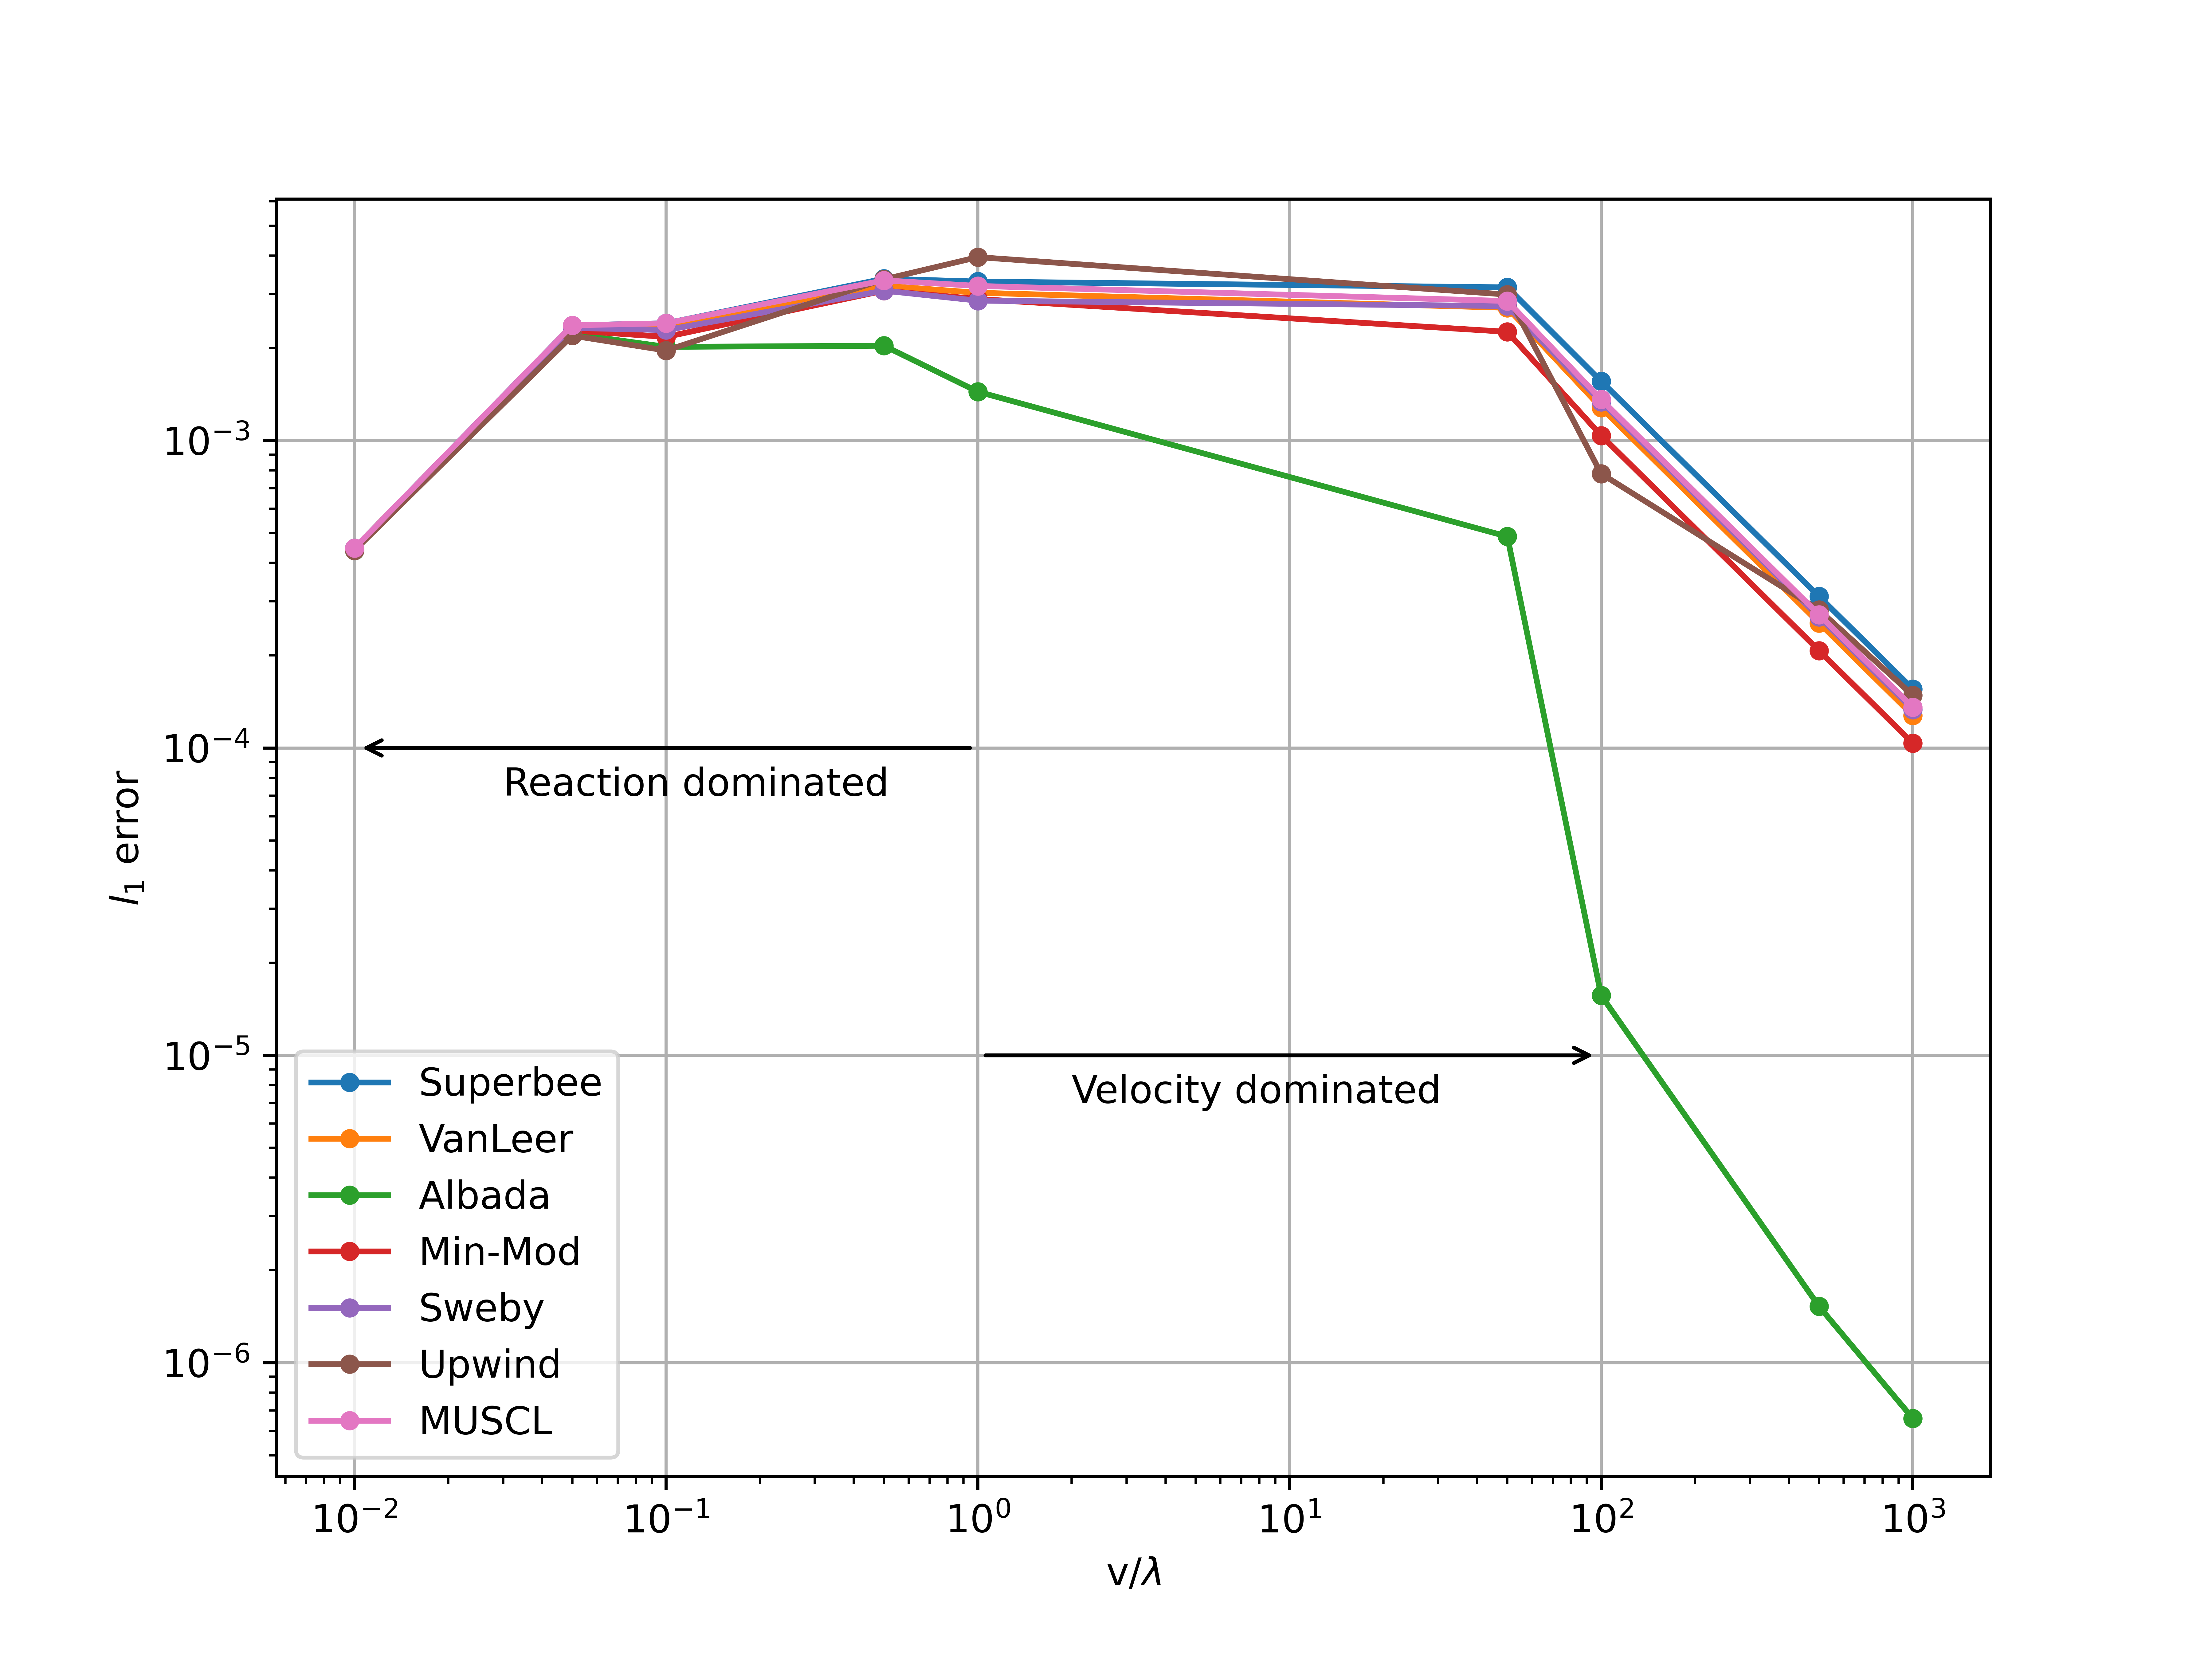
\includegraphics[width=6in]{images/chapter-5/progressionProblems/problem5/problem5CoefficientChanges.png}
    \caption{Problem 5 flux limiter relative E${}_{1}$ behavior with coefficient changes using absolute error}
    \label{fig:problem5_l1error_coefficient_changes}
\end{figure}

\clearpage

\begin{figure}[p]
    \centering
    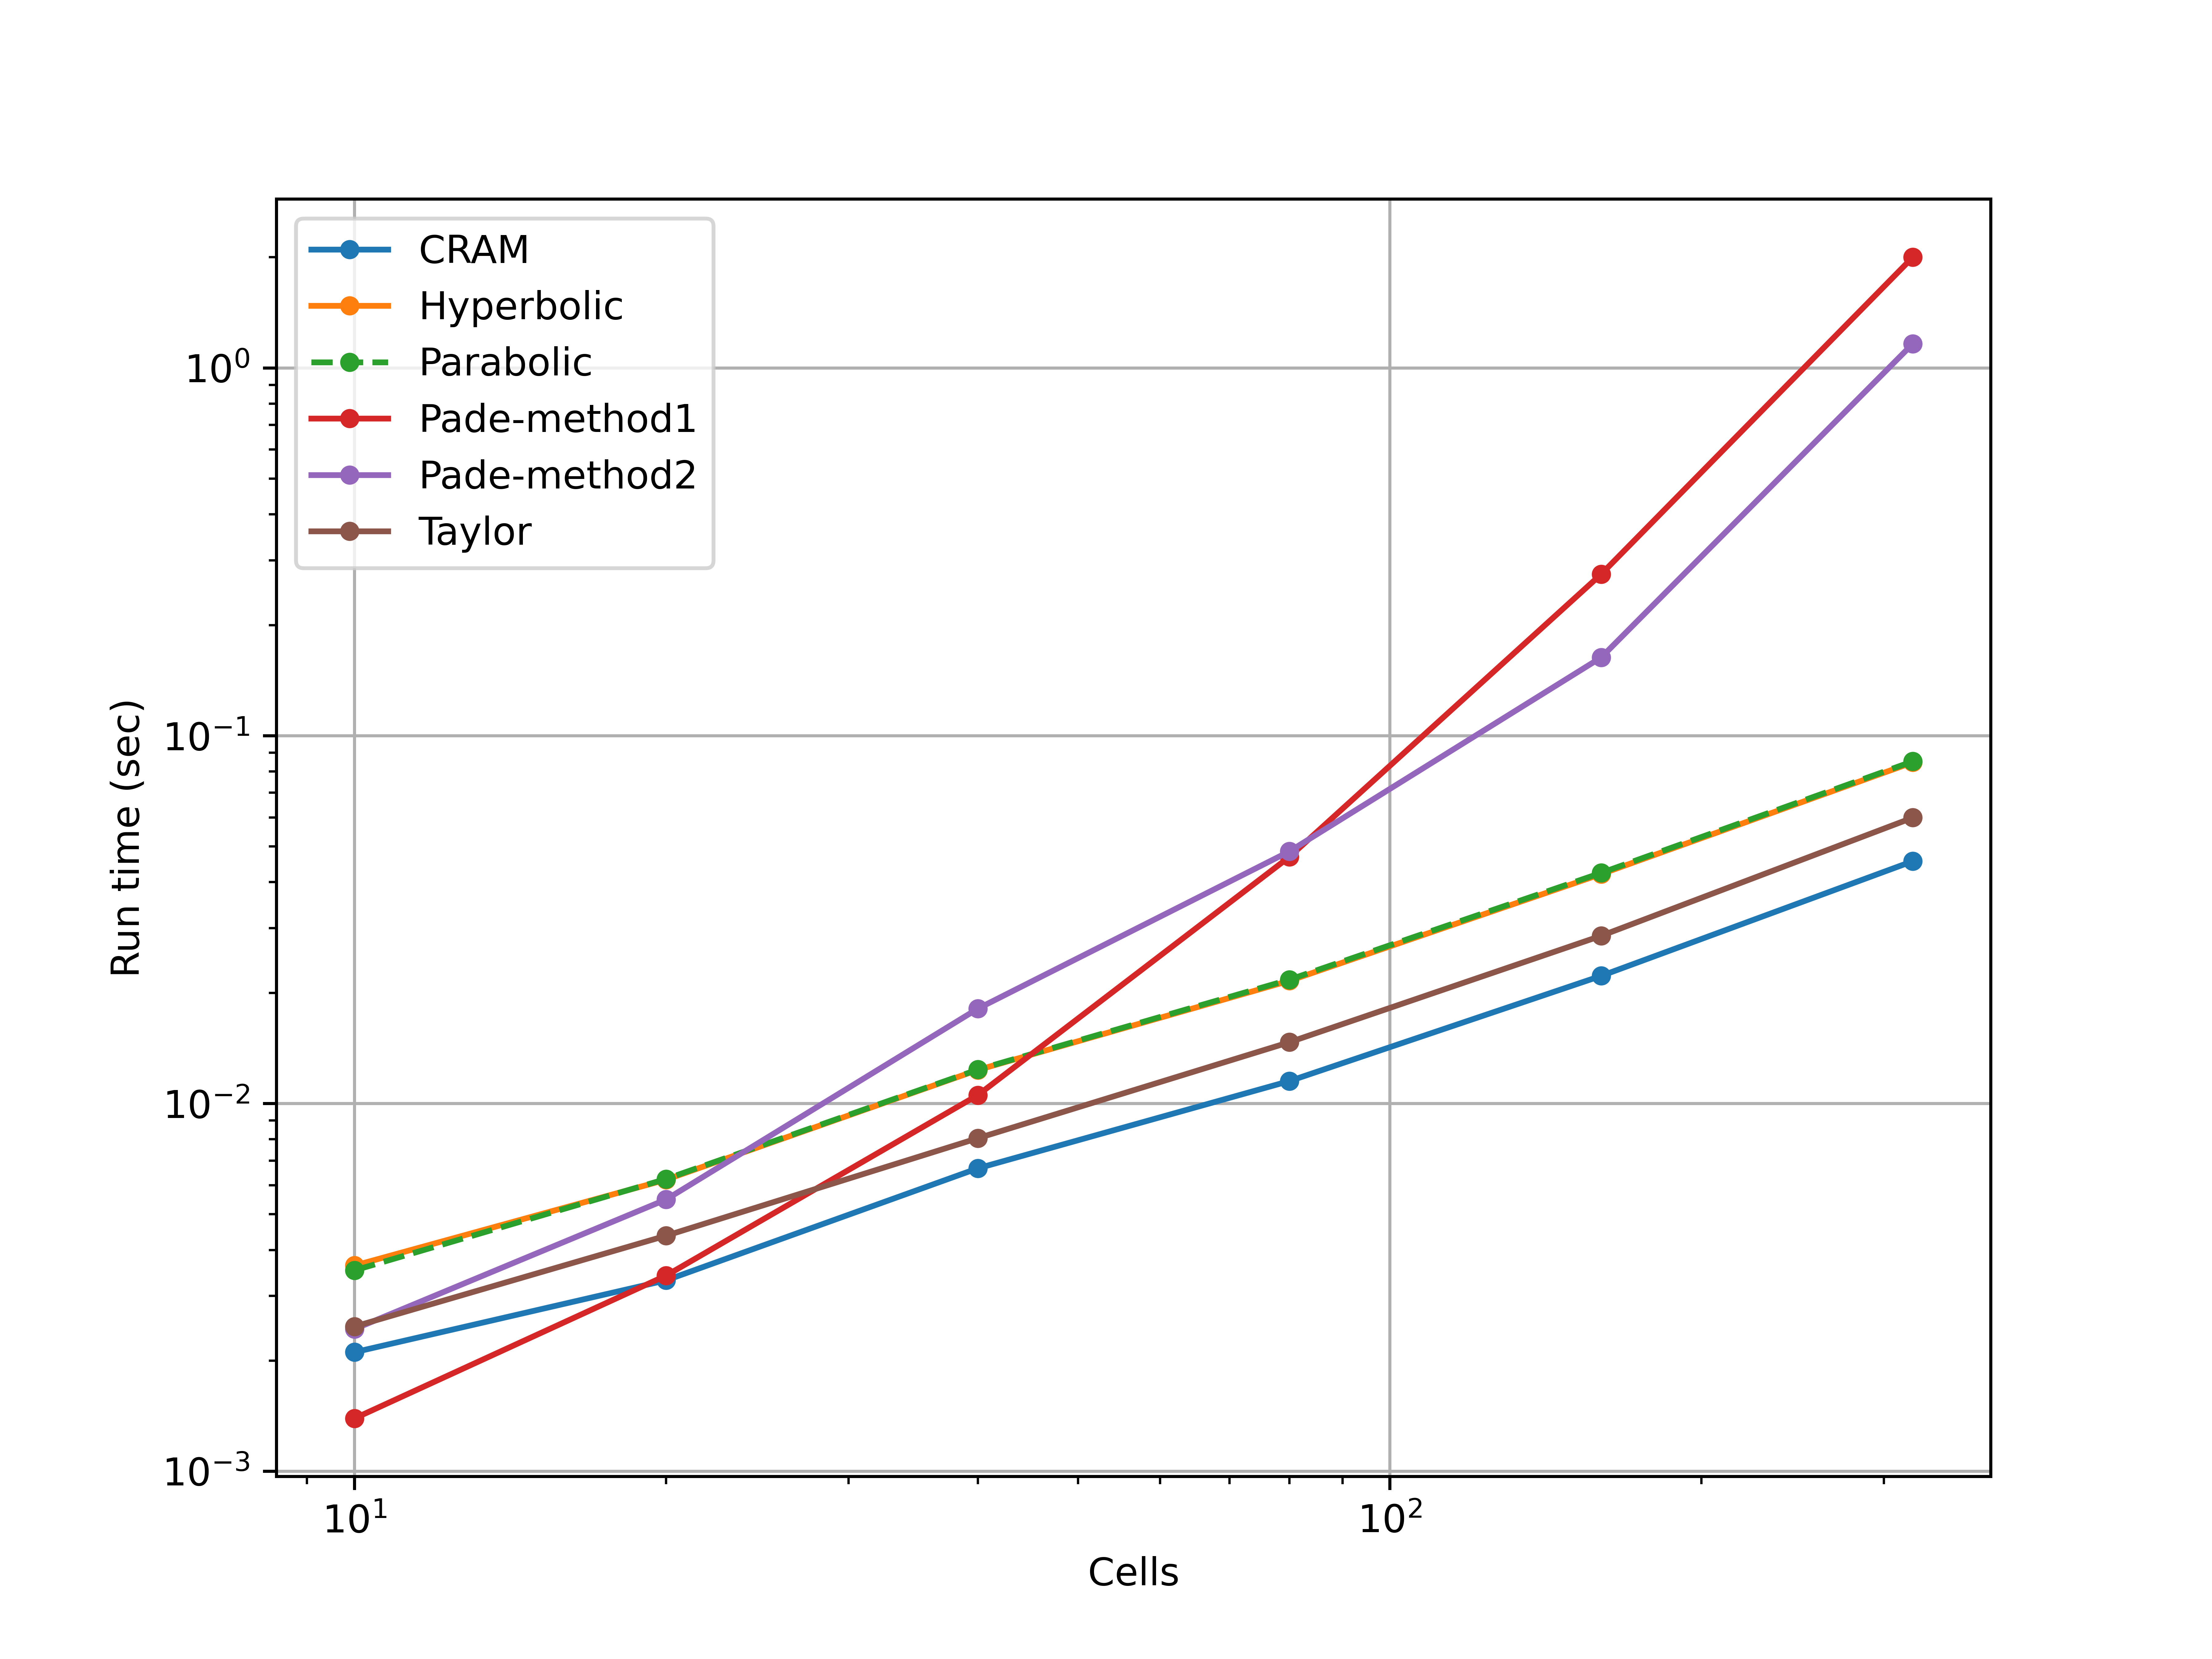
\includegraphics[width=6in]{images/chapter-5/progressionProblems/problem5/problem5Runtimes.png}
    \caption{Problem 5 average run times for each solver, dt = 0.1}
    \label{fig:problem5_runtimes}
\end{figure}

\clearpage

\subsection{Problem 6}
This is an extension of problem 6 with two species, one that exist in the liquid and one on the wall. The species in the liquid transports and depositions on the wall where it sticks and does not move. In libowski this is accomplished by excluding the loop which adds the convection contribution to the wall species. This system is represented by:

\begin{equation}
\setlength{\jot}{15pt}
\begin{split}
    &\frac{\partial C_{l}}{\partial t} = -v\frac{\partial C_{l}}{\partial x} - \frac{kA}{V} C_{l}, \\
    &\frac{\partial C_{w}}{\partial t} = \frac{kA}{V} C_{l},
    \label{eq:problem6}
\end{split}
\end{equation}

\noindent on the domain $x \in [0,100]$, $t \in [0, 20]$ where $v = 2$ and $kA/V = \lambda = 0.01$. Subject to the following conditions:

\begin{equation}
\setlength{\jot}{15pt}
\begin{split}
    C_{l}(x, 0) = 1000, \quad C_{l}(0,t) = 1000, \quad \frac{dC_{l}}{dx}(100, t) = 0, \\
    C_{w}(x, 0) = 0, \quad C_{w}(0,t) = 0, \quad \frac{dC_{l}}{dx}(100, t) = 0. \\
\end{split}
\end{equation}

\noindent Let $\lambda = kA/V$, equation \ref{eq:problem6} the following solution:

\begin{equation}
C_{l} (x,t) = \begin{cases}
  C_{l} (x, 0) e^{-\frac{x \lambda _i}{v}}\ , & x < vt \\
  C_{l} (x, 0) e^{-t \lambda _i}\ , & x \ge vt
\end{cases}
\end{equation}

\begin{equation}
C_{w} (x,t) = \begin{cases}
  C_{l} (x, 0) \Big( 1 - e^{-\frac{x \lambda _i}{v}} + \lambda \big(t - x/v\big)e^{-\lambda x/v} \Big)\ , & x < vt \\
  C_{l} (x, 0) \Big( 1 - e^{-t \lambda _i}\Big)\ , & x \ge vt
\end{cases}
\end{equation}

This problem is conducted in the same manor as problem 4 and 5. But unlike problem 4, this problem has a discontinuous solution. Figures \ref{fig:problem6_l1error_spatial_results} and  \ref{fig:problem6_l1error_time_results} shows results for the E${}_{1}$ error as a function of time and space. These results shows the same behavior for each of the flux limiters that was shown in problem 4. The only difference is the error is slightly higher in this problem. Again, the Albada flux limiter showes the lowest over all error and does show the most improvement from increasing the number of time steps. Figure \ref{fig:problem6_linferror_spatial_results} and \ref{fig:problem6_linferror_time_results} shows that the E${}_{\infty}$ error follows the same shape from problem 5. For high dt, each of the flux limiters seem to converge to the same solution. As the time step size is decreased, each flux limiter begins to separate, with Albada acheiving the lowest error for low dt and dx. Figure \ref{fig:problem6_linferror_time_results} shows that for a high dx, increasing the number of time steps causes most of the high order flux limiter functions to become worst. As dx becomes lower, all of the high order functions become more accurate until they reach a point where decreasing dt does not affect the solution. The Albada limiter however, increases its accuracy as dt decreases for all dx values. Figures \ref{fig:problem6_l2error_spatial_results} and \ref{fig:problem6_l2error_time_results} show that the E${}_{2}$ also behaves the same in problems 5 and 6. For a low number of cells, each of the limiter functions converge to a similar solution, with the Albada limiter out performing the rest. 

Figure \ref{fig:problem6_l1error_fluxlimiter_convergence_rate} shows the spatial convergence rate as a function of space and time. This figure shows the same convergence behavior seen in problem 5, but with slightly different values. In this case, the Albada limiter shows a higher convergence rate, while each of the other limiters seem to have higher convergence rates for higher dt. As the number of steps is increased the convergence rates are higher in problem 5. Figures \ref{fig:problem6_linferror_fluxlimiter_convergence_rate} and \ref{fig:problem6_l2error_fluxlimiter_convergence_rate} show the spatial convergence rates for the E${}_{\infty}$ and E${}_{2}$. Both of these figures show the same trend that was seen in problem 5. The E${}_{\infty}$ error shows low convergence rates for the Albada and Min-Mod limiters, while the other limiters have high convergence rates for both low dt and dx. The E${}_{2}$ error shows higher convergence rates for all limiters for both low dt and dx. 

Figure \ref{fig:problem6_l1error_coefficient_changes} shows E${}_{1}$ error with changes in the problem coefficients. This figure shows almost the exact same behavior that was seen in problem 5. In a reaction dominated system, all limiters converge to the same solution. As the velocity is increased, each of the limiters separate, with the Albada limiter performing the best. Figure \ref{fig:problem6_runtimes} shows run times for this problem behave in a similar way to problem 5. However in problem 6, the Taylor, Hyperbolic and Parabolic solvers have almost the same run times.

\clearpage

\begin{figure}[p]
    \centering
    \includegraphics[width=6in]{images/chapter-5/progressionProblems/problem6/problem6E1ErrorWithSpace.png}
    \caption{Problem 6 relative E${}_{1}$ error with spatial discretization at various time steps}
    \label{fig:problem6_l1error_spatial_results}
\end{figure}

\clearpage

\begin{figure}[p]
    \centering
    \includegraphics[width=6in]{images/chapter-5/progressionProblems/problem6/problem6E1ErrorWithTime.png}
    \caption{Problem 6 relative E${}_{1}$ error with temporal discretization at various number of spatial cells}
    \label{fig:problem6_l1error_time_results}
\end{figure}

\clearpage

\begin{figure}[p]
    \centering
    \includegraphics[width=6in]{images/chapter-5/progressionProblems/problem6/problem6E1FluxLimiterConvergenceRate.png}
    \caption{Problem 6 flux limiter relative E${}_{1}$ spatial convergence rate}
    \label{fig:problem6_l1error_fluxlimiter_convergence_rate}
\end{figure}

\clearpage

\begin{figure}[p]
    \centering
    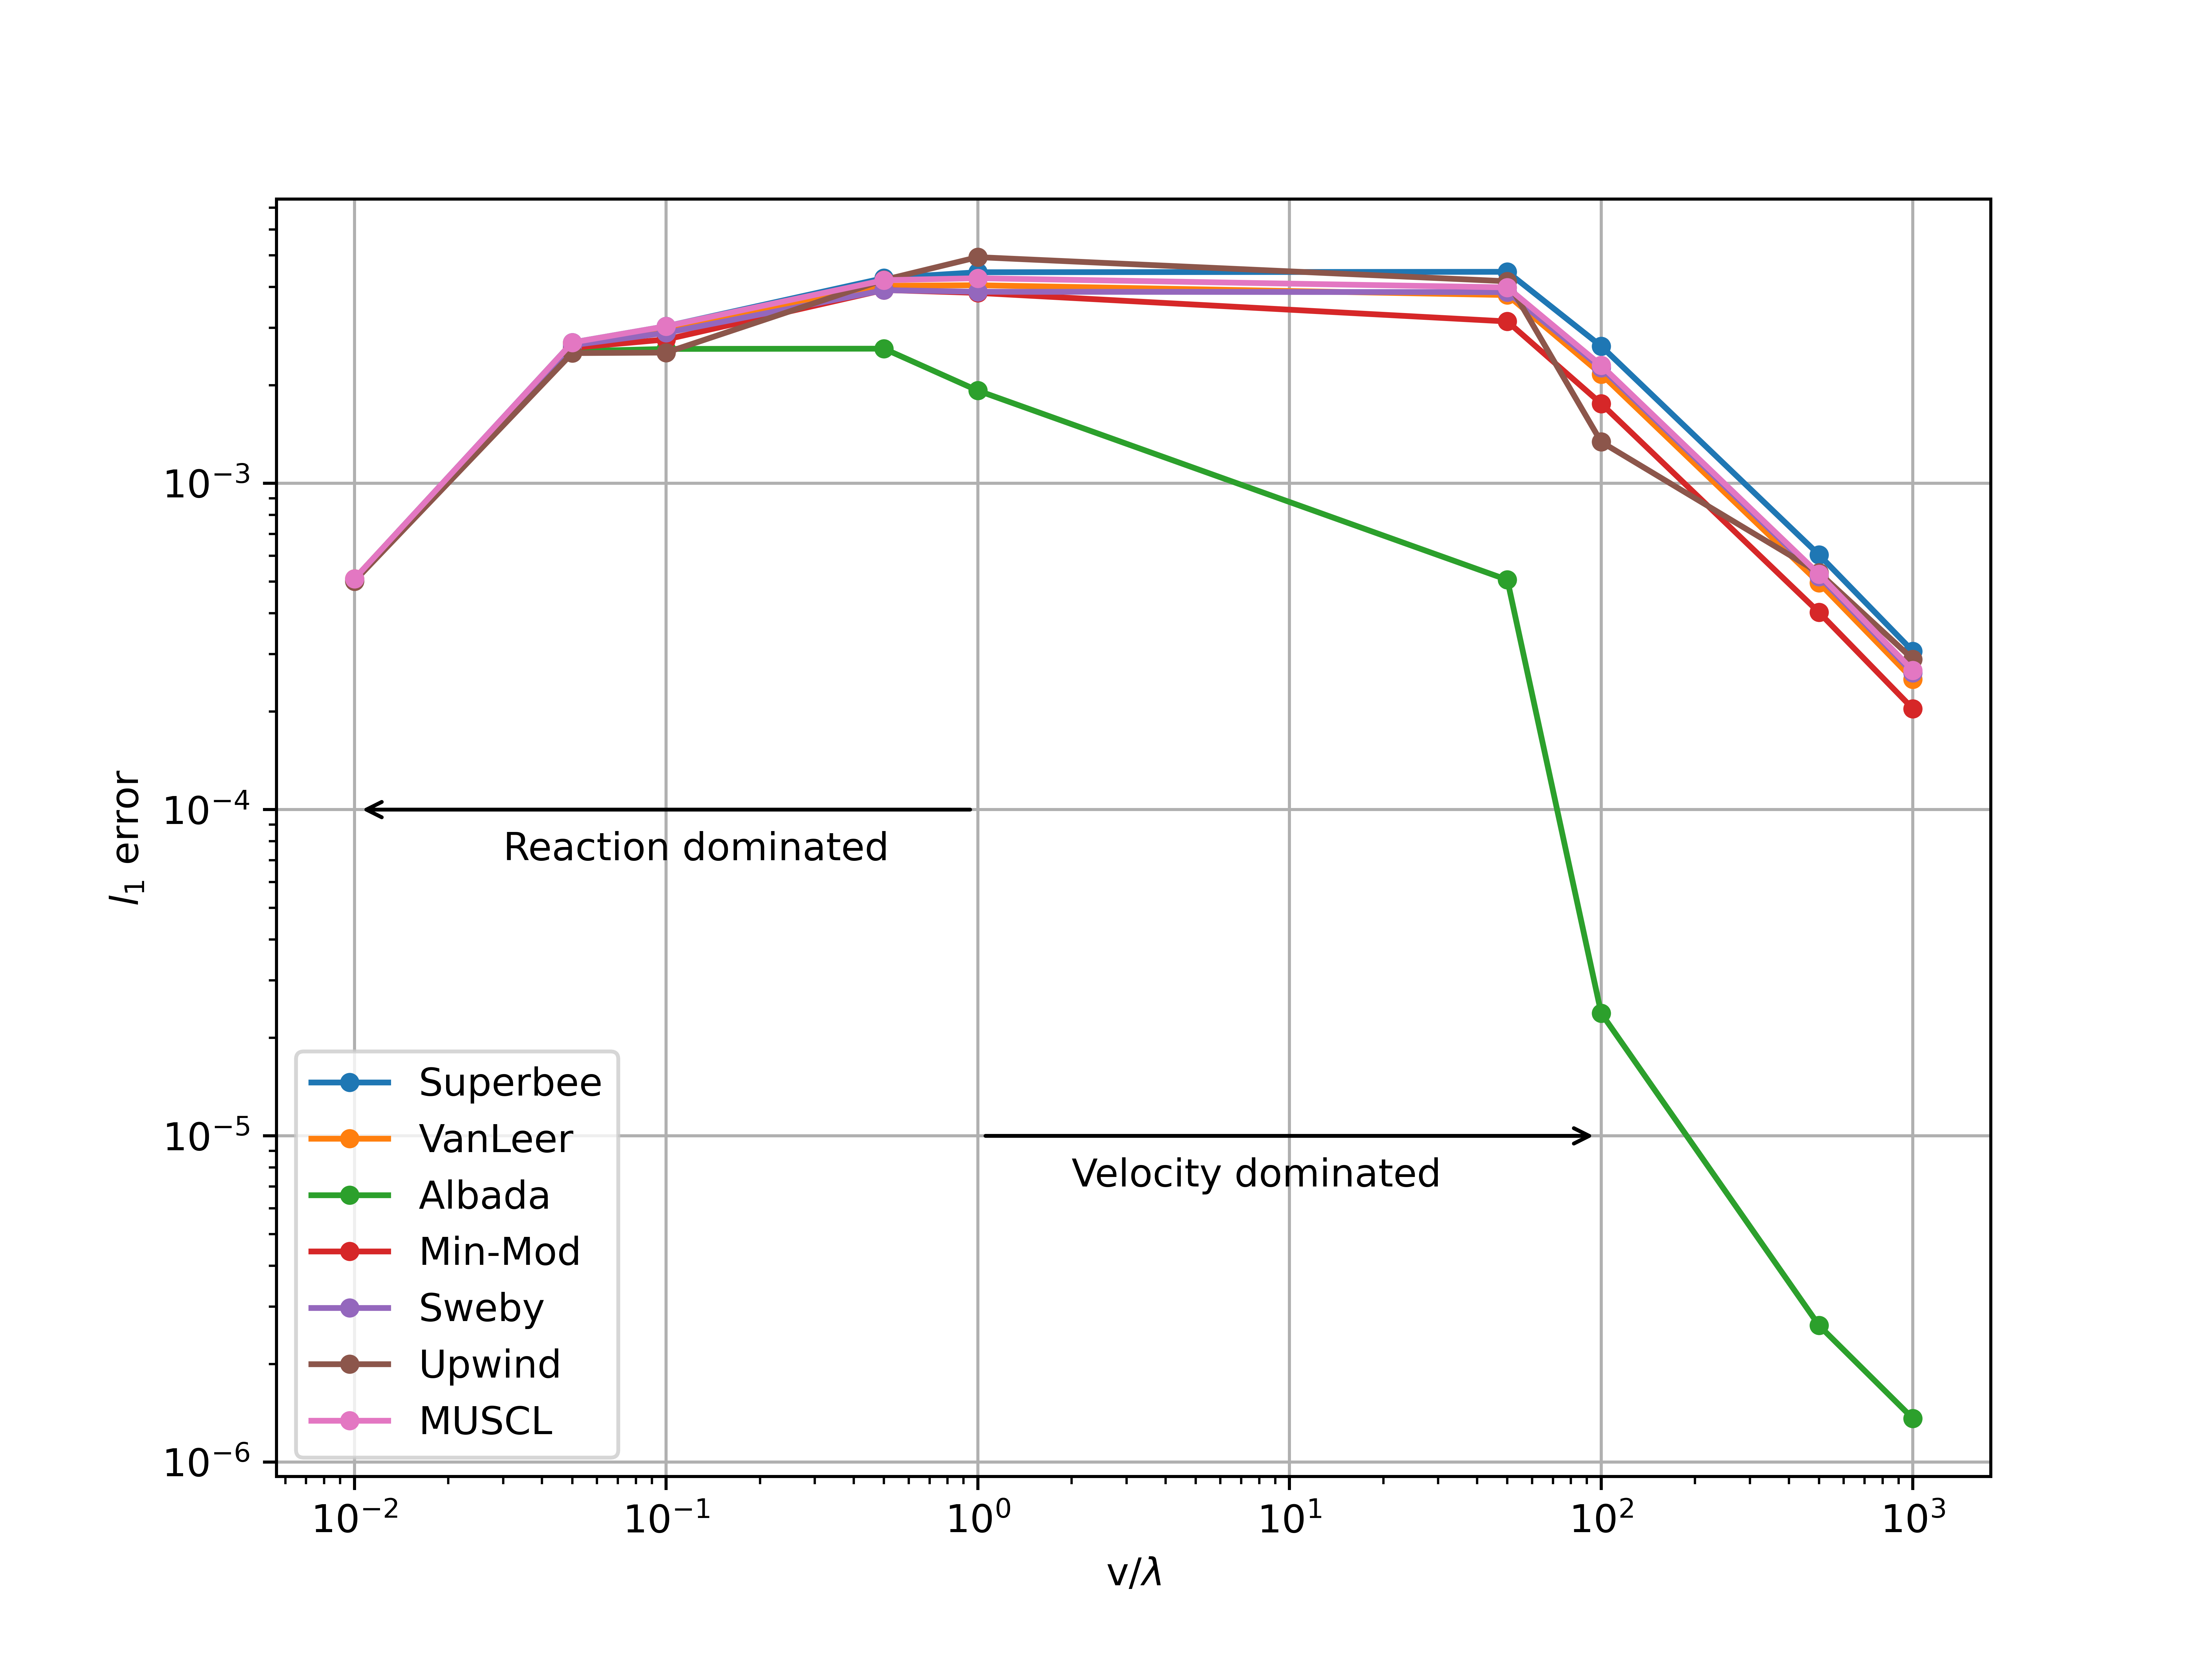
\includegraphics[width=6in]{images/chapter-5/progressionProblems/problem6/problem6CoefficientChanges.png}
    \caption{Problem 6 flux limiter relative E${}_{1}$ behavior with coefficient changes}
    \label{fig:problem6_l1error_coefficient_changes}
\end{figure}

\clearpage

\begin{figure}[p]
    \centering
    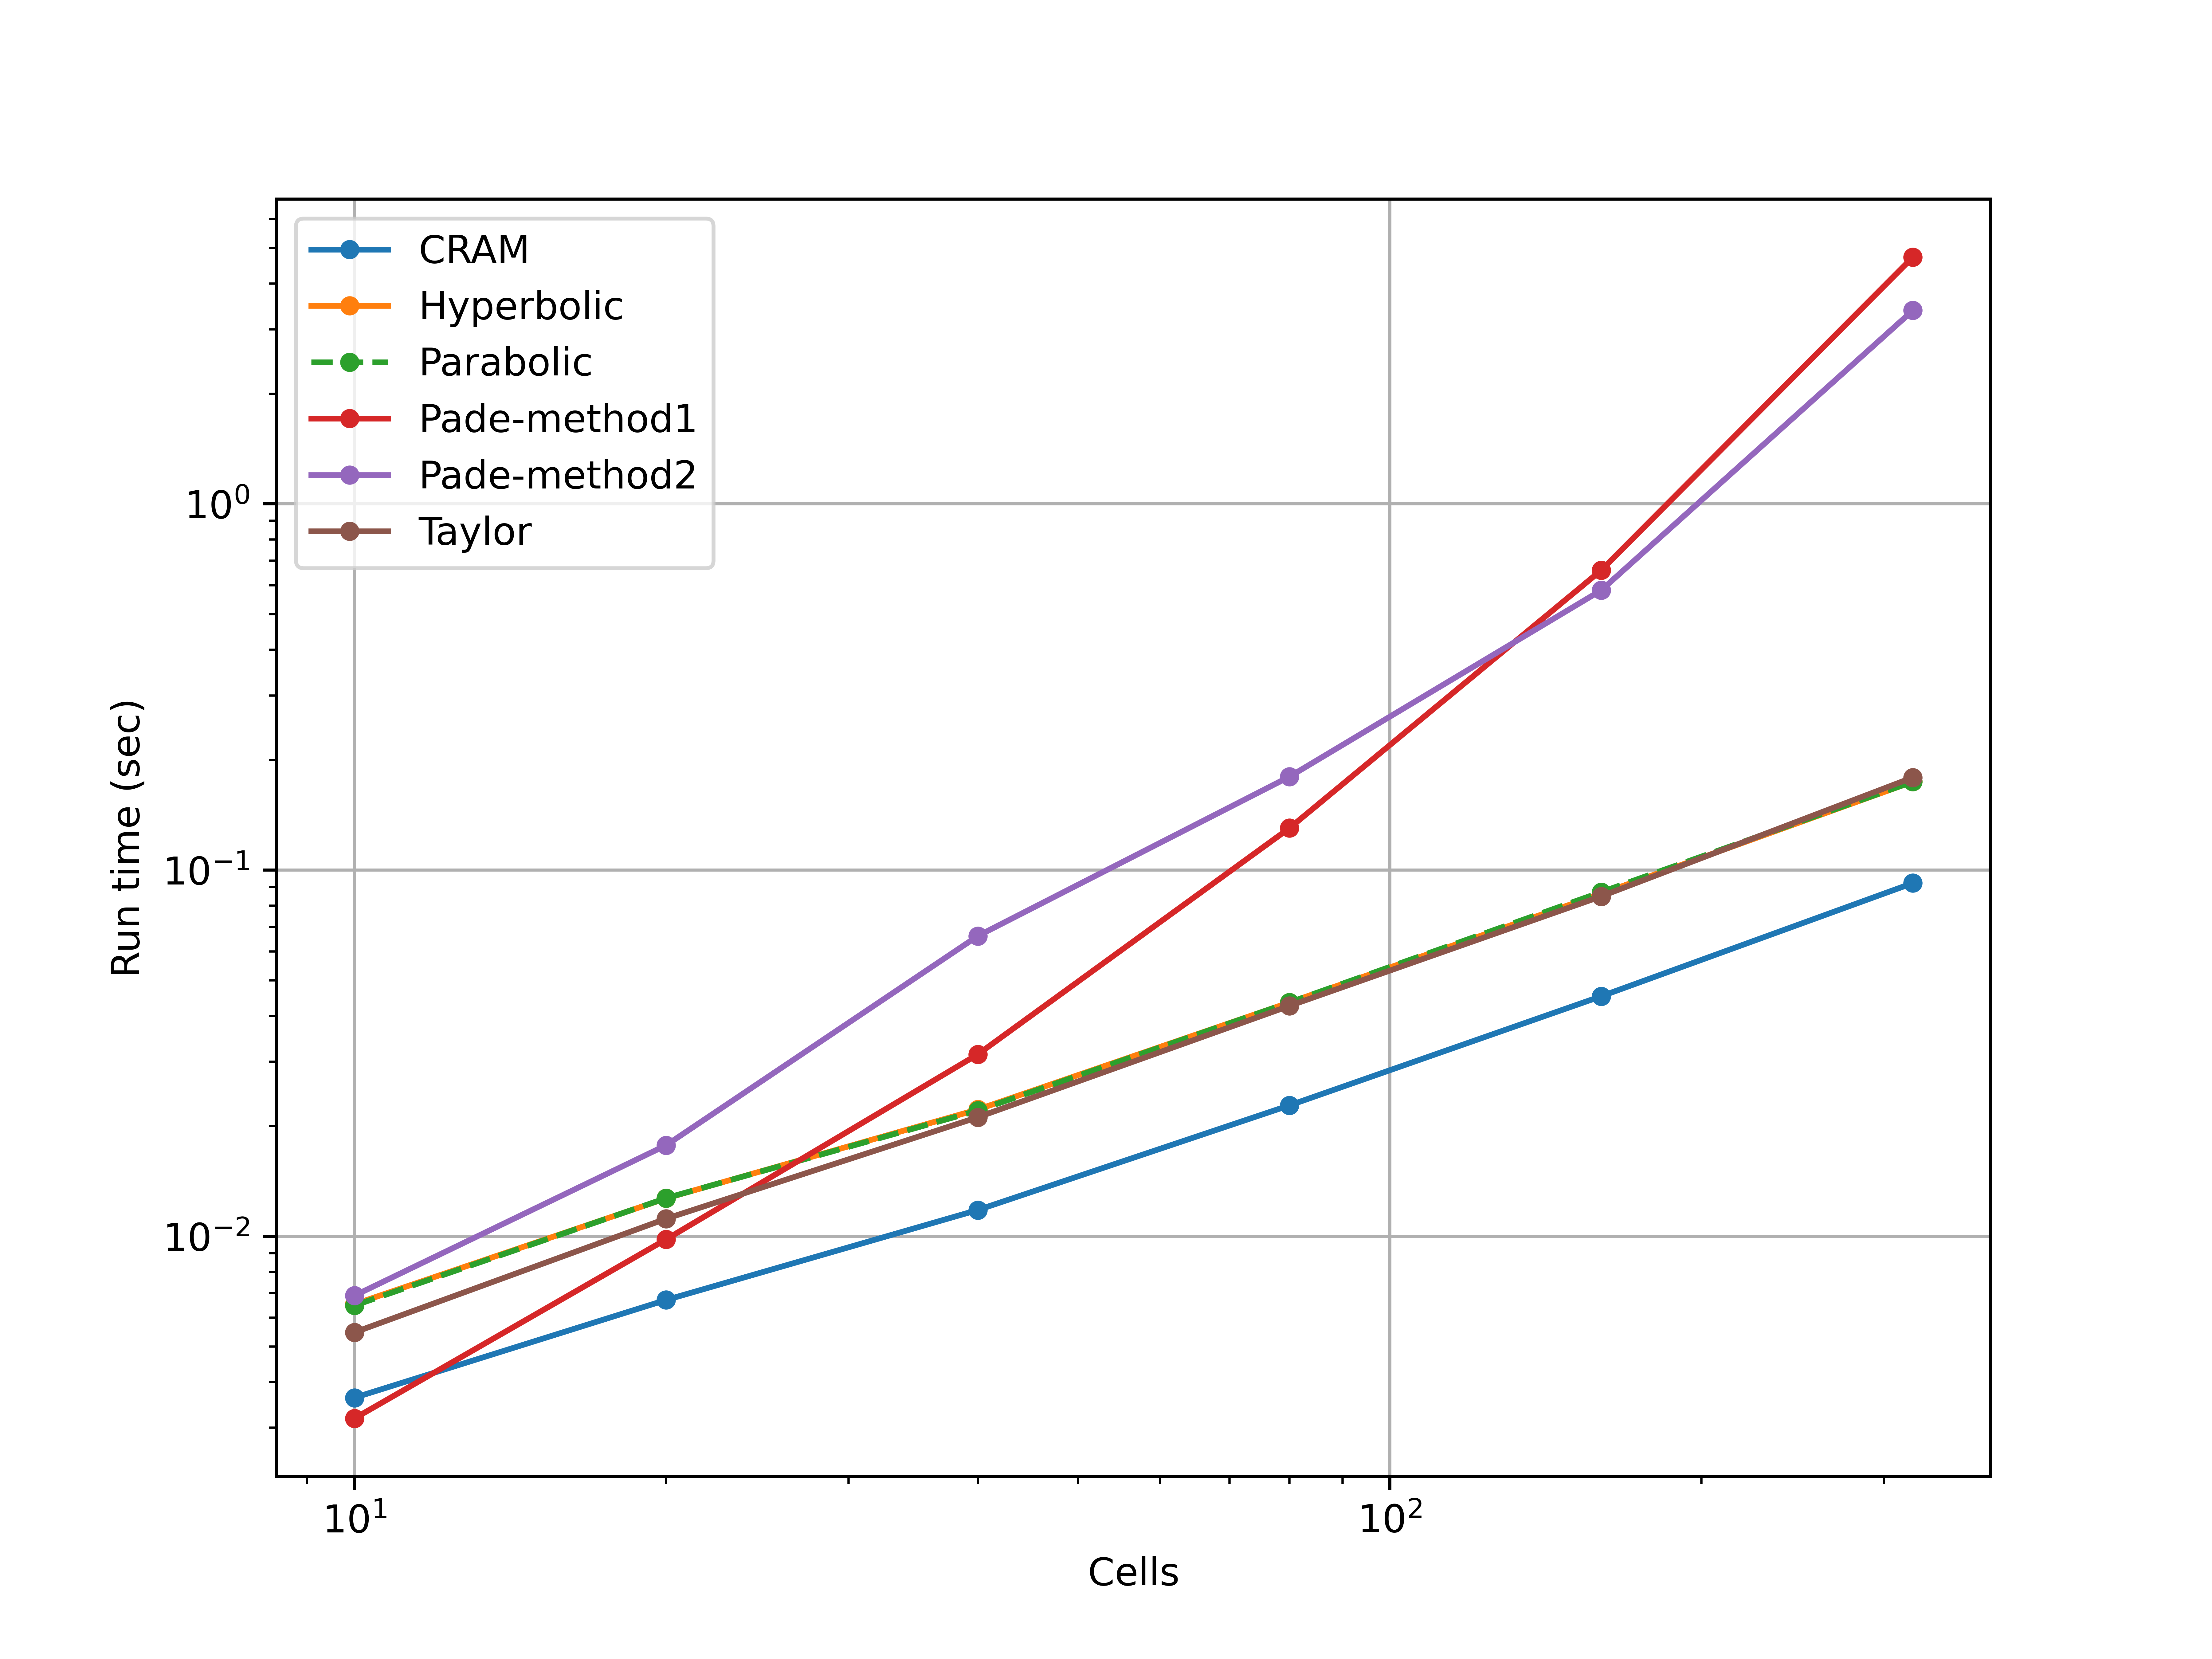
\includegraphics[width=6in]{images/chapter-5/progressionProblems/problem6/problem6Runtimes.png}
    \caption{Problem 6 average run times for each solver, dt = 0.1}
    \label{fig:problem6_runtimes}
\end{figure}

\clearpage

\subsection{Problem 7}
This problem models the primary uranium isotopes along with Pu-239 and Np-239 in a system which contains a neutron flux. Coefficients in the transition matrix include source and sink terms from both neutron induced reactions and radioactive decay. This system is represented by:


\begin{equation}
\frac{d C_i}{dt} = \sum^9_{j = 1} A_{ij} C_j (x, t)
\end{equation}

\begin{equation}
i = \begin{dcases}
  1 , & \text{$^{233}$U}  \\
  2 , & \text{$^{234}$U}  \\
  3 , & \text{$^{235}$U}  \\
  4 , & \text{$^{236}$U}  \\
  5 , & \text{$^{237}$U}  \\
  6 , & \text{$^{238}$U}  \\
  7 , & \text{$^{239}$U}  \\
  8 , & \text{$^{239}$Pu} \\
  9 , & \text{$^{239}$Np} \\
\end{dcases}
\end{equation}

\noindent On the domain from $t \in [0, 500]$ subject to the following neutron flux $\phi = 1e13$ n/cm$^2/$/s. Each isotope is given an initial concentration of $C_{i, 0} = 1e10$ atoms/cm$^2$. The transition matrix is built using information from the SCALE ORIGEN library. The analytical solution is given by the exponential of the transition matrix:

\begin{equation}
   \boldsymbol{C}(t) = e^{\boldsymbol{A}t}, 
\end{equation}

\noindent where $\boldsymbol{C}$ is a vector of isotope concentrations. The solution is calculated using in MATLAB using the method previously described. This solution is plotted in figure \ref{fig:problem7_solution}, with a zoomed in portion showing the solution for a number of the isotopes are very close. 

\clearpage

\begin{figure}[p]
    \centering
    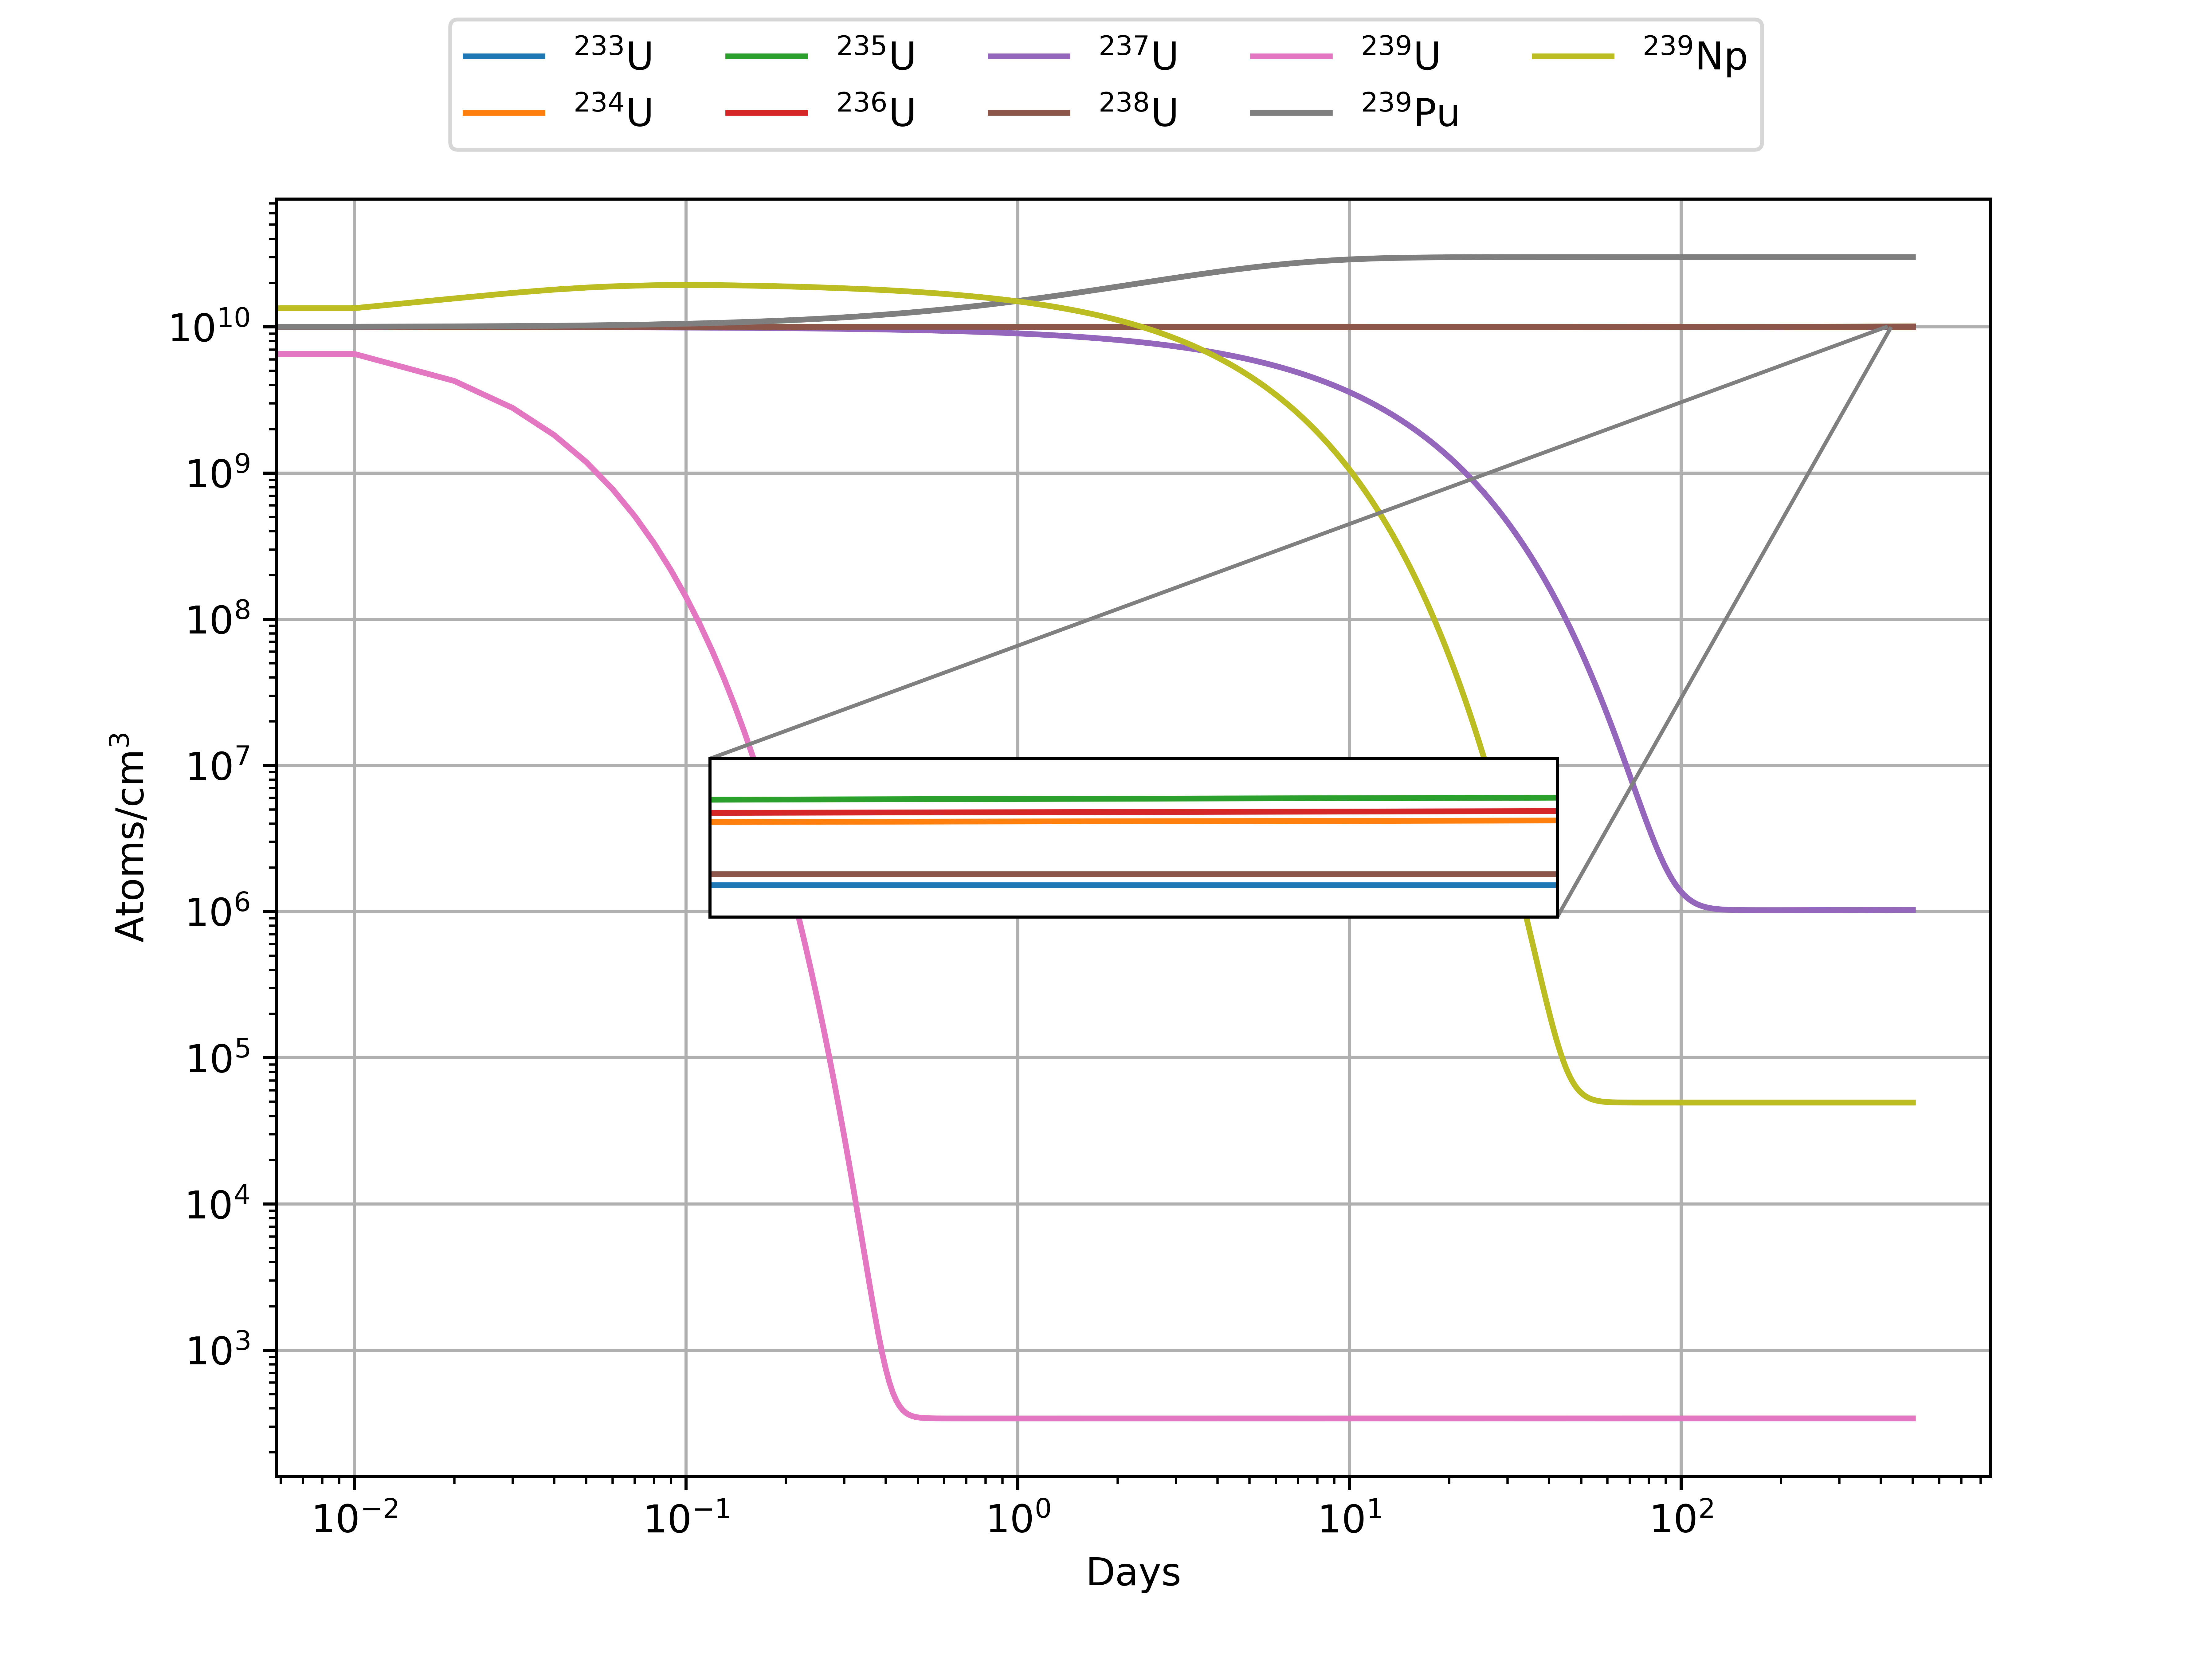
\includegraphics[width=6in]{images/chapter-5/progressionProblems/problem7/problem7soltution.png}
    \caption{Problem 7 solution}
    \label{fig:problem7_solution}
\end{figure}

\clearpage

This problem offers a good example of how sub-stepping can be utilized in improving the solution for Cauchy solvers.  Results of the sub-stepping for the Cauchy solvers are shown in Figure \ref{fig:problem7_E1_error_with_steps} at the 50-day time step mark. Surprisingly, CRAM started out with the largest E${}_{1}$ relative error. With just 2 substeps, the error from all Cauchy solvers dropped by many orders of magnitude. Past 4 substeps, the errors begin to compound from an inaccurate initial condition. While the behavior in this system shows that 6 is the optimal number of sub-steps for the CRAM and Hyperbolic solvers and 2 for the Parabolic solver. Error behavior for E${}_{\infty}$ and E${}_{2}$ are shown in Appendix \ref{appen:results}, figures \ref{fig:problem7_Einf_error_with_steps} and \ref{fig:problem7_E2_error_with_steps}. Figure \ref{fig:problem7_Einf_error_with_steps} shows the same trend but with a minimal value at 4 steps instead of 6 for CRAM and Hyperbolic. Figure \ref{fig:problem7_E2_error_with_steps} shows the same behavior that was seen with the E${}_{1}$ error. 

Results for the decay transition matrix are shown in Figure \ref{fig:problem7_E1_error_with_steps4}, where each Cauchy solver was run with 4 substeps. Both the CRAM and hyperbolic solvers outperformed the other solvers. The parabolic solver, the Taylor solver, and the Pad\'e-method 1 solver all performed about the same. The Pad\'e-method 2 solver performed the worst, but the E${}_{1}$ relative error was still below $10^{-9}$ over the solution domain. Results for E${}_{\infty}$ and E${}_{2}$ are shown in figures \ref{fig:problem7_Einf_error_with_steps4} and \ref{fig:problem7_E2_error_with_steps4}, these results show the same trends seen in figure \ref{fig:problem7_E1_error_with_steps4}. 


Run times for all of these solvers were quite fast and are shown in Table \ref{tab:problem7_run_times}; Cauchy solvers are shown for 4 sub-steps. For a test as small as the one analyzed here, all run times were remarkably fast. While the $l_{l}$ matrix norm is ~2,100 for the time step size and requires a notable amount of scaling, the problem was small enough that it did not increase the run times for series solvers. 

Eigenvalues for this problem are shown in figure \ref{fig:problem7_eigenvalues}, while most have zero for the imaginary parts there are two which have non zero elements. However, these eigenvalues are still clustered extremely close to the zero axis and do not affect the accuracy of the Cauchy solvers by themselves. While the accuracy of the Cauchy solvers are not affected by the placement of the eigenvalues, it is however, affected by the change is nuclide concentration over the time steps involved. Figure \ref{fig:problem7_nuclide_relative_error} shows the relative error of each nuclide at the 50 day time step for each of the Cauchy solvers. This figure, along with figure \ref{fig:problem7_solution} shows that the nuclides contributing to the highest two errors are the ones whos solution changes the most during that time step. 

\clearpage

\begin{figure}[p]
    \centering
    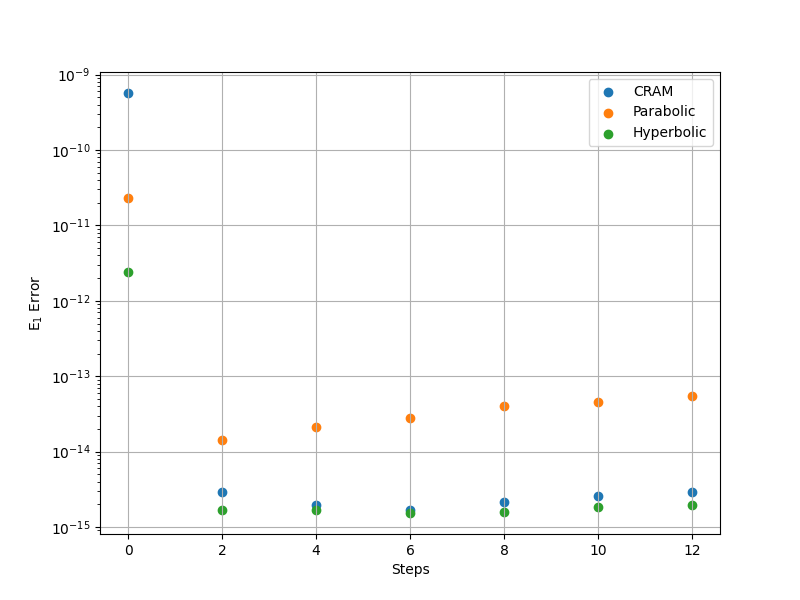
\includegraphics[width=6in]{images/chapter-5/progressionProblems/problem7/problem7E1ErrorWithSteps.png}
    \caption{Problem 7 E${}_{1}$ relative error with sub-steps}
    \label{fig:problem7_E1_error_with_steps}
\end{figure}

\clearpage

\begin{figure}[p]
    \centering
    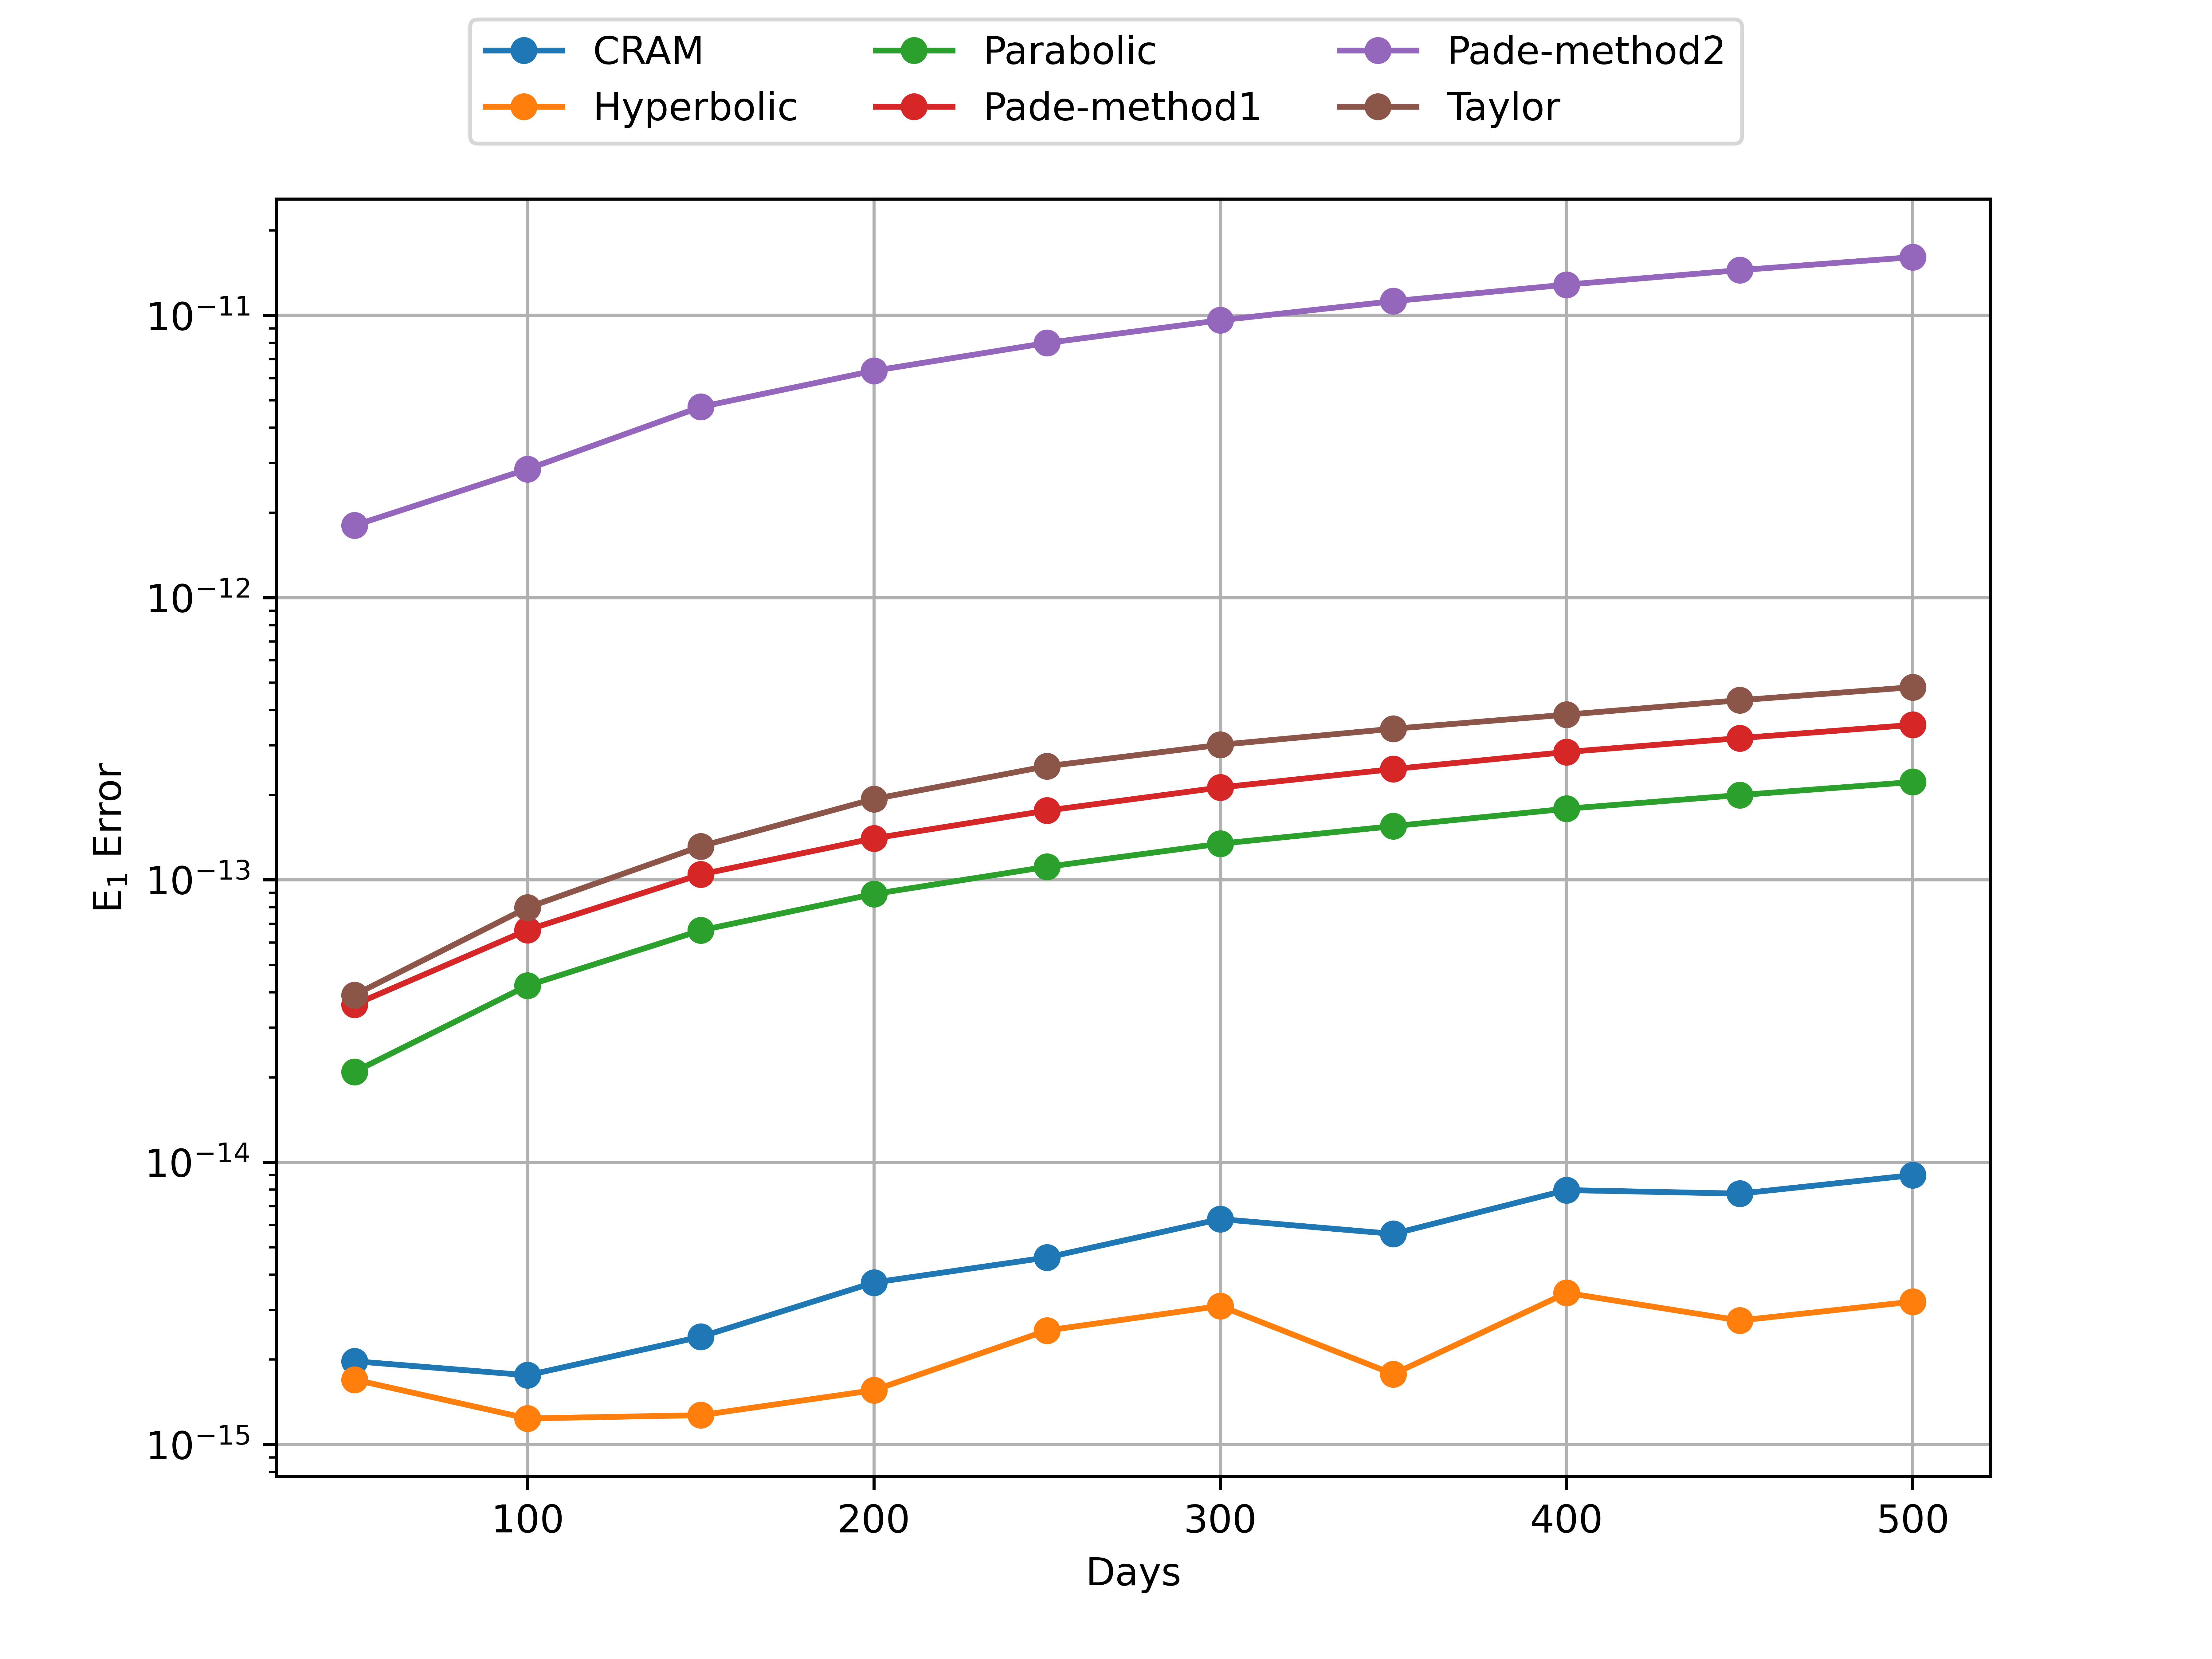
\includegraphics[width=6in]{images/chapter-5/progressionProblems/problem7/problem7E1ErrorerrorSteps4.png}
    \caption{Problem 7 E${}_{1}$ relative error with 4 sub-steps}
    \label{fig:problem7_E1_error_with_steps4}
\end{figure}

\clearpage

\begin{table}[p]
   \caption{\label{tab:problem7_run_times} Run Times for All Solvers in Depletion Case}
   \centering
   \begin{tabular}{ll}
   \hline
   Solver & Run time (sec)  \\
   \hline
   CRAM & 9.04e-03 \\
   Hyperbolic & 1.51e-02 \\
   Parabolic & 1.51e-02 \\
   Pad\'e-method 1 & 1.09e-03 \\
   Pad\'e-method 2 & 2.29e-03 \\
   Taylor & 5.76e-03 \\
   \hline
   \end{tabular}
\end{table}  

\clearpage

\begin{figure}[p]
    \centering
    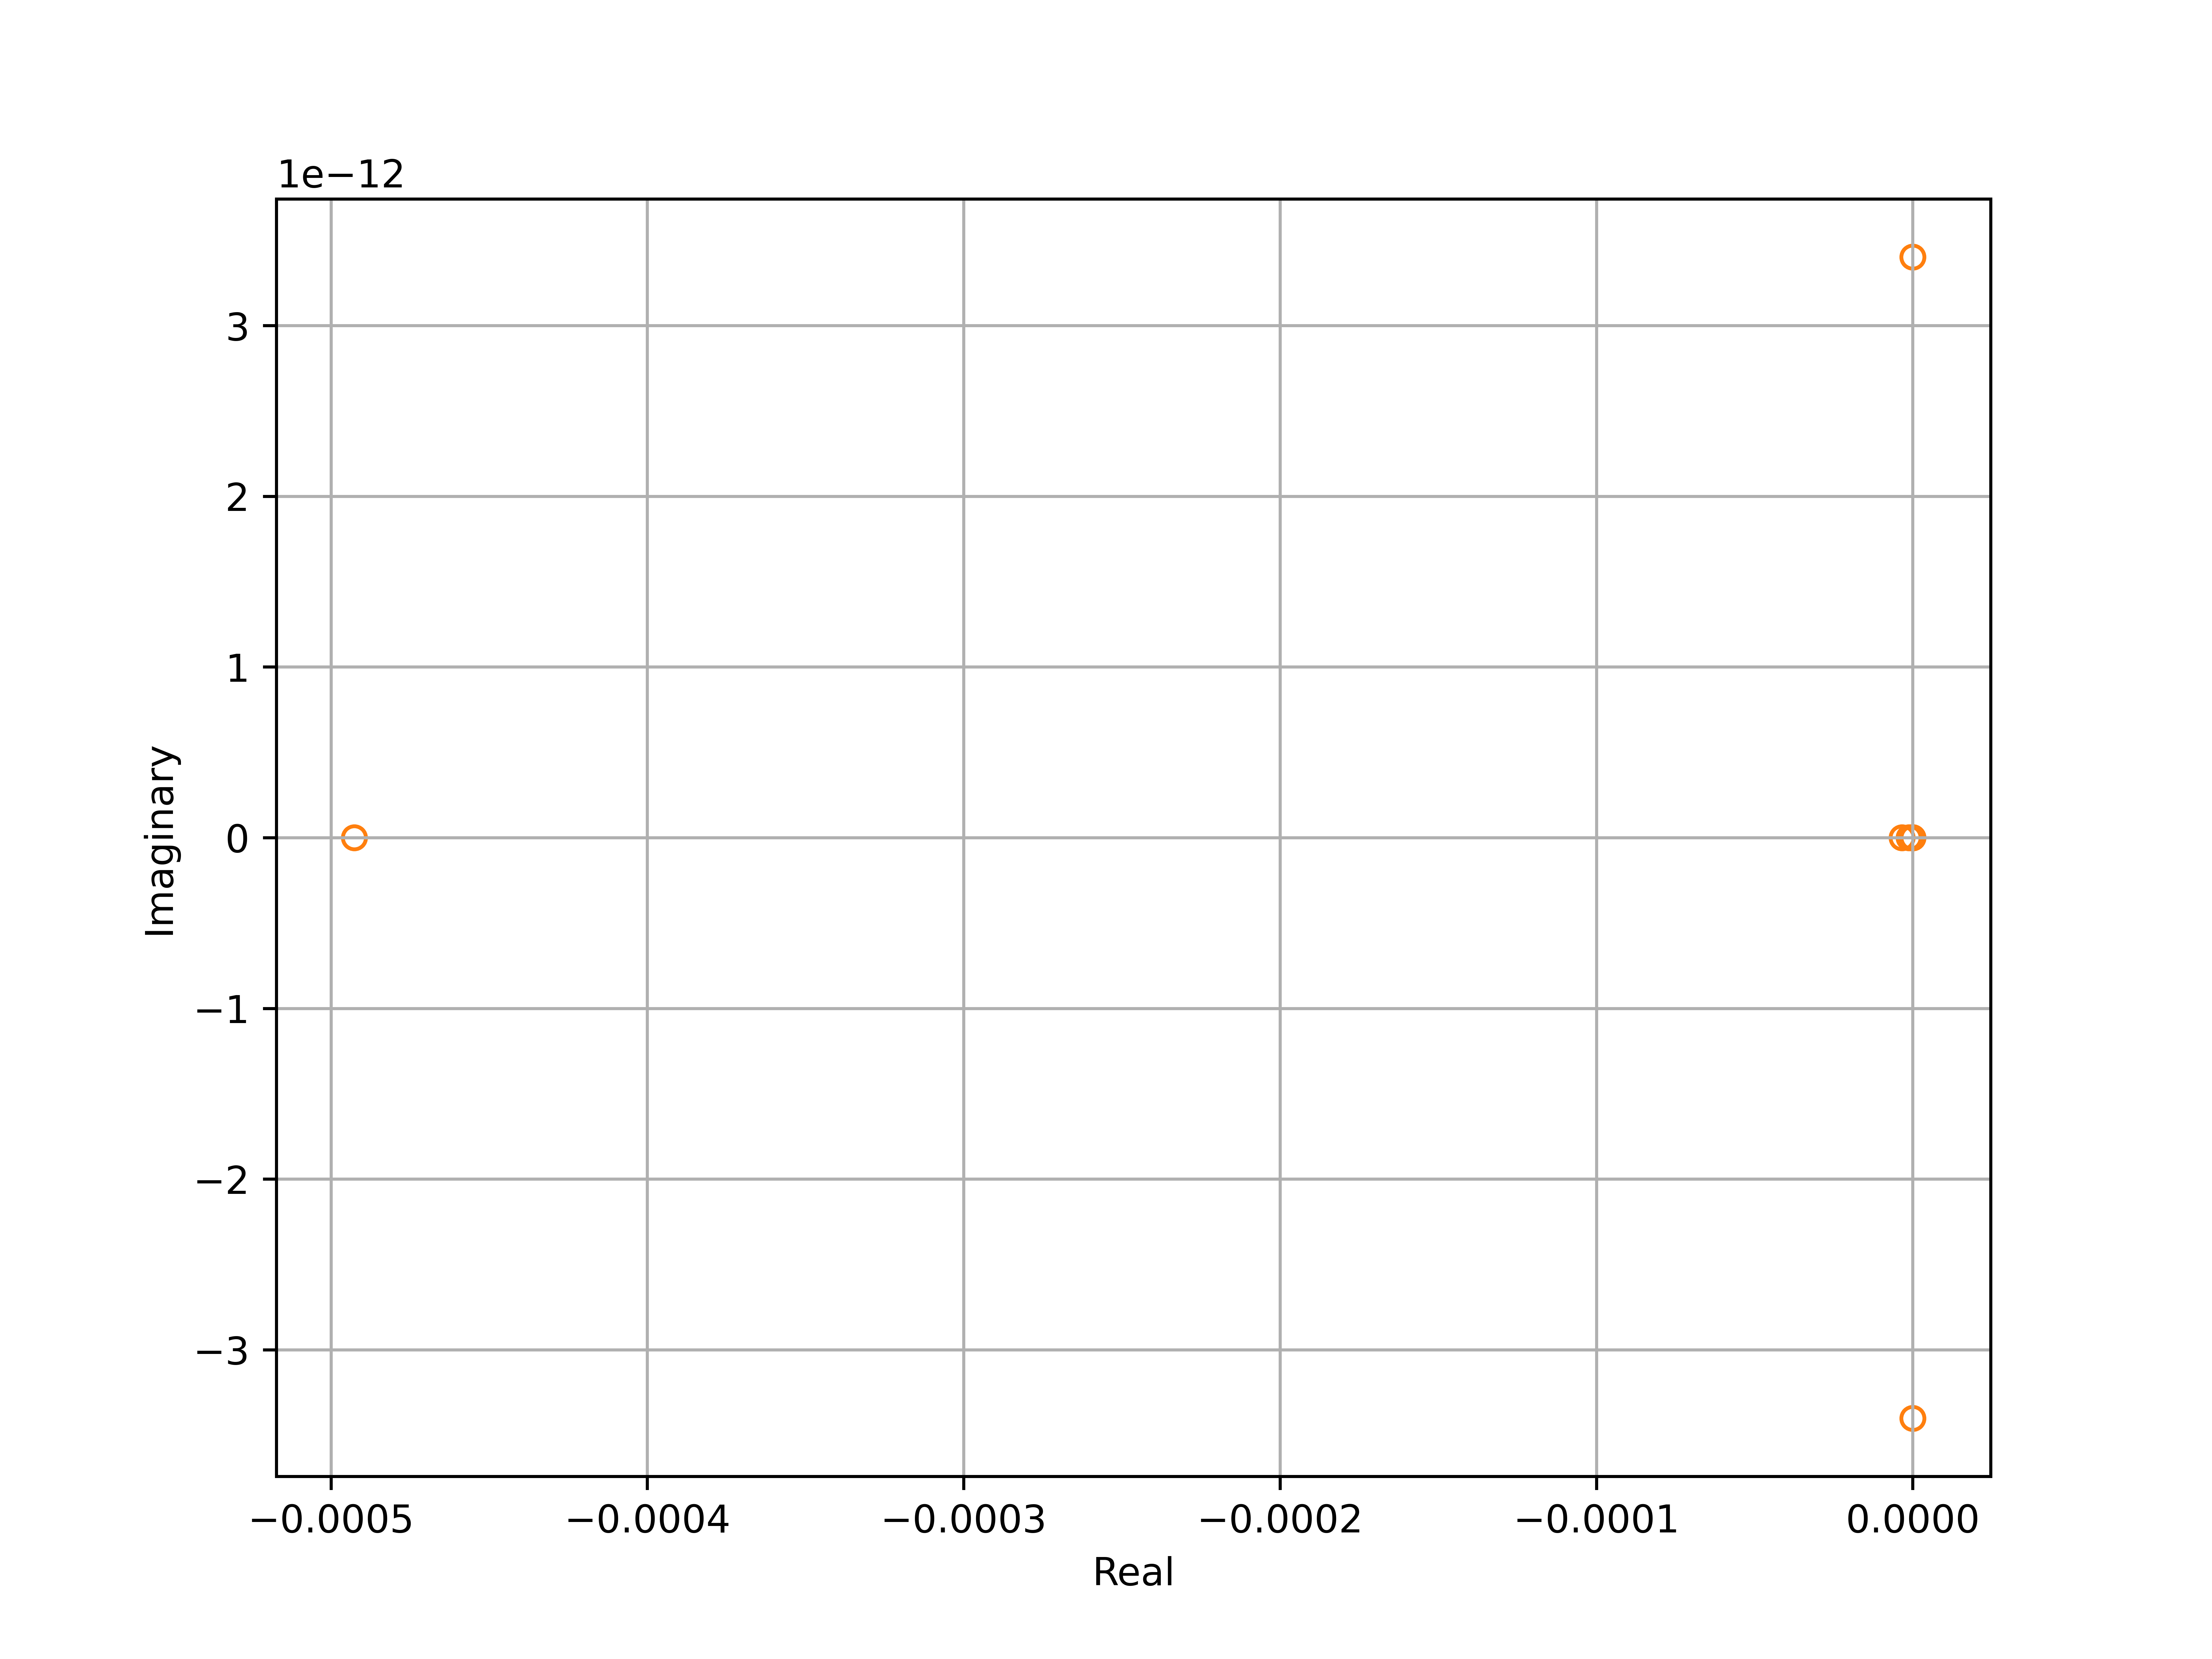
\includegraphics[width=6in]{images/chapter-5/progressionProblems/problem7/problem7Eigenvalues.png}
    \caption{Problem 7 eigenvalues}
    \label{fig:problem7_eigenvalues}
\end{figure}

\clearpage

\begin{figure}[p]
    \centering
    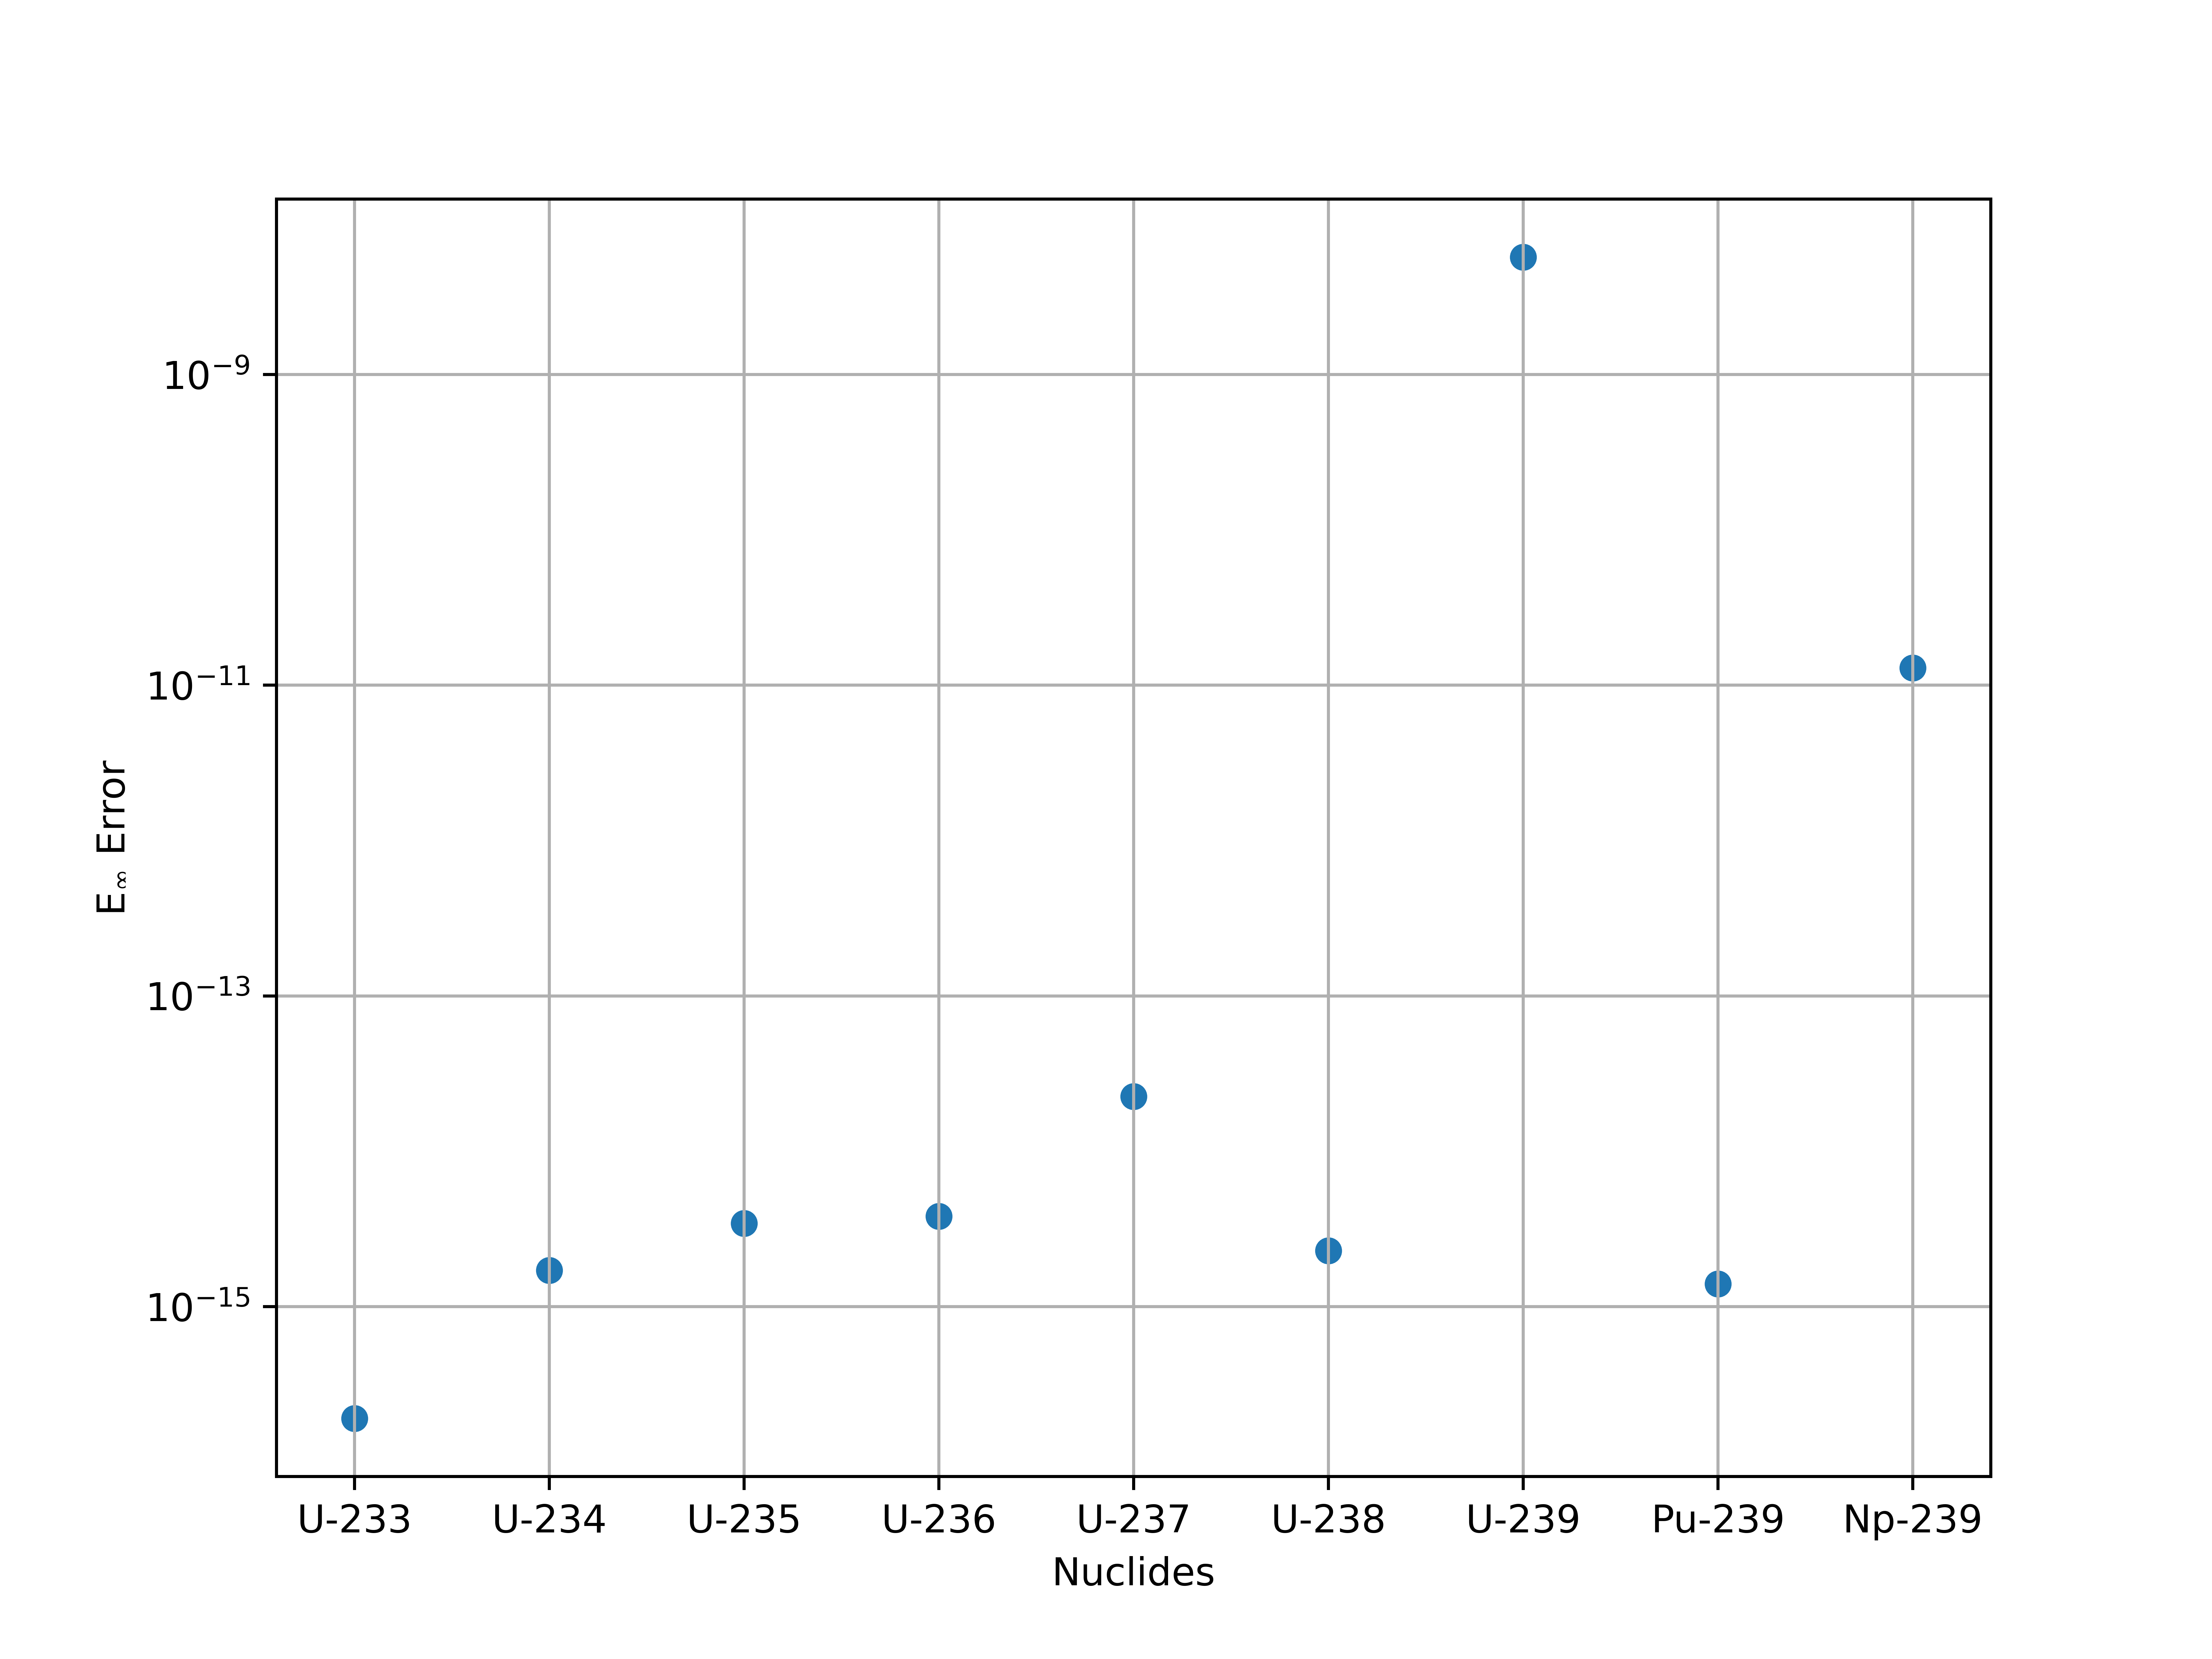
\includegraphics[width=6in]{images/chapter-5/progressionProblems/problem7/problem7NuclideErrorFirstStep.png}
    \caption{Problem 7 E${}_{\infty}$ relative error for each nuclide at the first time step}
    \label{fig:problem7_nuclide_relative_error}
\end{figure}

\clearpage

\subsection{Problem 8}
This is an extension of problem 9 but for a fictitious "pipe" reactor which allows for the flow of isotopes due to a velocity. This is represented by:

\begin{equation}
\frac{d C_i}{dt} = -v\frac{\partial C_{i}}{\partial x} + \sum^9_{j = 1} A_{ij} C_j (x, t)
\end{equation}

\begin{equation}
i = \begin{dcases}
  1 , & \text{$^{233}$U}  \\
  2 , & \text{$^{234}$U}  \\
  3 , & \text{$^{235}$U}  \\
  4 , & \text{$^{236}$U}  \\
  5 , & \text{$^{237}$U}  \\
  6 , & \text{$^{238}$U}  \\
  7 , & \text{$^{239}$U}  \\
  8 , & \text{$^{239}$Pu} \\
  9 , & \text{$^{239}$Np} \\
\end{dcases}
\end{equation}

\noindent On the domain $x \in [0, 400]$, $t \in [0, 500]$. Subject to the periodic boundary conditions:

\begin{equation}
    C_{i}(0,t) = C_{i}(400,t).
\end{equation}

\noindent The neutron flux follows a sine function in the x-direction from $x \in [0, 200]$, half of the total length of the pipe. Four different velocities are chosen $ v = 2, 25, 50 $ and $100$, with a time step size of 50 days. This problem is ran with 3 different discretization sizes, with the number of cells varying from 10, 20 and 40. The higher order flux limiter functions are not used, with the first order upwind function being chosen for the convective flux. The reference solution is calculated using MATLAB. The eigenvalues for each velocity and discretization are shown in figure \ref{fig:problem8_eigenvalues}, the left column are the eigenvalues of the transition matrix and the right column are the eigenvalues of the transition matrix multiplied by the time step size. As the number of cells increases the real and imaginary parts of the eigenvalues spread further out. This also happens as the velocity is increased. 

\clearpage

\begin{figure}[p]
    \centering
    \includegraphics[width=6in]{images/chapter-5/progressionProblems/problem8/problem8Eigenvalues.png}
    \caption{Problem 8 eigenvalues for each velocity and discretization}
    \label{fig:problem8_eigenvalues}
\end{figure}

\clearpage

The E${}_{1}$ error for each velocity are shown for cells 10, 20 and 40 in figures \ref{fig:problem8_E1_error_10cells}, \ref{fig:problem8_E1_error_20cells} and \ref{fig:problem8_E1_error_40cells}. Figure \ref{fig:problem8_E1_error_10cells} shows that all solvers but Pad\'e-method2 have around the same error. As the velocity is increased the error increases, with errors for velocities of 50 and 100 appear to be on top of one another except for Pad\'e-method2. Figure \ref{fig:problem8_E1_error_20cells} shows that for 20 cells, E${}_{1}$ errors for velocities 25, 50 and 100 fall on top of one another. Pad\'e-method1 again shows the worst error, with this error increasing as a function of velocity. Figure \ref{fig:problem8_E1_error_40cells} shows that the error for velocities 25 and 50 are about the same for all but Pad\'e-method2 and Taylor. Error for a velocity of 50 is only slightly higher than 25. Again Pad\'e-method2 shows the worst error, with the error increases with velocity. An important take away from these results is that each solver shows the same error behavior as a function of velocity. Indicating that the increased error seen in the Cauchy solvers do not result from the placement of the eigenvalues. Results for both the E${}_{\infty}$ and E${}_{2}$ errors for 10, 20 and 40 cells are shown in Appendix \ref{appen:results}, figures \ref{fig:problem8_Einf_error_10cells}, \ref{fig:problem8_Einf_error_20cells}, \ref{fig:problem8_Einf_error_40cells}, \ref{fig:problem8_E2_error_10cells}, \ref{fig:problem8_E2_error_20cells} and \ref{fig:problem8_E2_error_40cells}. These error metrics show the same behavior as E${}_{1}$. 

Run times for each solver using 40 cells are shown for each velocity in Table \ref{tab:}, each of the Cauchy solvers are shown with 2 sub-steps. None of the Cauchy solvers appear to show variation in run time with increased velocity but there is some slight differences with the Pad\'e solvers. The Taylor solver is most effected by the change in velocity and the reason is found in the scaling and squaring method itself. 

\clearpage

\begin{figure}[p]
    \centering
    \includegraphics[width=6in]{images/chapter-5/progressionProblems/problem8/problem8E1ErrorWithVelocity10cells.png}
    \caption{Problem 8 E${}_{1}$ error with 10 cells}
    \label{fig:problem8_E1_error_10cells}
\end{figure}

\clearpage

\begin{figure}[p]
    \centering
    \includegraphics[width=6in]{images/chapter-5/progressionProblems/problem8/problem8E1ErrorWithVelocity20cells.png}
    \caption{Problem 8 E${}_{1}$ error with 20 cells}
    \label{fig:problem8_E1_error_20cells}
\end{figure}

\clearpage

\begin{figure}[p]
    \centering
    \includegraphics[width=6in]{images/chapter-5/progressionProblems/problem8/problem8E1ErrorWithVelocity40cells.png}
    \caption{Problem 8 E${}_{1}$ error with 40 cells}
    \label{fig:problem8_E1_error_40cells}
\end{figure}

\clearpage

\section{Case Studies}
The following are a selection of case studies which aim to explore libowskis' accuracy and performance with problems which come up in modeling MSRs. 

\subsection{Neutron precursors}
This problem examines a convection-driven flow with the 6 neutron precursor groups, as shown in Eqs. (\ref{eq:problem3}) and (\ref{eq:problem3flux}): 

\begin{equation}
\frac{\partial C_{i}}{\partial t} = -v_{x}\frac{\partial C_{i}}{\partial x} - v_{y}\frac{\partial C_{i}}{\partial y} + \beta_{i} \Psi (x, y) -\lambda_i C_{i},
\label{eq:problem3}
\end{equation}

\begin{equation}
\Psi (x, y) = \begin{cases}
  \psi _0 \sin\left(\frac{\pi x}{50}\right)\sin\left(\frac{\pi y}{100}\right) , x \in [0,50], y \le 100 \\
  0\ , \text{otherwise},
  \label{eq:problem3flux}
\end{cases}
\end{equation}

\noindent where $i \in [1,6]$, $x \in [0, 50]$, $y \in [0, 400]$, $t \in [0, 60]$, $v_{x} = 0$, and $v_{y} = 25$, subject to the following boundary conditions:

\begin{equation}
    C_{i}(x,0) = C_{i}(x,400), \quad \frac{dC_{i}}{dx}(0,y) = 0, \quad \frac{dC_{i}}{dx}(50, y) = 0.
\end{equation}

Coefficients for the system are shown in Table \ref{tab:precursorCoeffs} \cite{ott1985}. 
Each precursor had the same initial condition of zero, and the source term for each precursor was scaled in the x and y directions by the sine function. The spatial domain was modeled to mimic an MSR with a core region extending from $y \in [0,100]$ and $x \in [0,50]$, with a core exterior loop modeled from $y \in [100, 400]$. 

\begin{table}[h!]
   \caption{\label{tab:precursorCoeffs} Parameters for Neutron Precursors}
   \centering
   \begin{tabular}{lll}
   \hline
   Group & $\lambda$ & $\beta$ \\
   \hline
   1 & 0.0127 & 0.0006 \\
   2 & 0.0317 & 0.00364 \\
   3 & 0.115 & 0.00349 \\
   4 & 0.311& 0.00628 \\
   5 & 1.4 & 0.00179\\
   6 & 3.87 & 0.0007 \\
   \hline
   \end{tabular}
\end{table}     

While there is no analytic solution for this example problem, a reference solution was generated in Matlab using the symbolic tool box to solve for the matrix exponential. A small, spatially discretized problem was set up with 5 cells in the x direction and 20 in the y direction. The transition matrix that was built was then exported to Matlab, and the matrix exponential was solved at various times and saved as the reference solution. While the spatial accuracy was not tested in this case, this method will access the accuracy of each matrix exponential algorithm. To further simplify the problem, the first-order upwind difference scheme was applied to the convective flux.

One important feature for many of these solvers was the location of the eigenvalues for the transition matrix. The spectrum was calculated using the Matlab symbolic tool box and is plotted in Figure \ref{fig:spectrum_neutron_precursors} for dx = 10, dy = 20, and various values of dt. Figure \ref{fig:spectrum_neutron_precursors} show 6 elliptical rings, one at each dt, each one representing a precursor group. For a given time step size, the eigenvalues shifted along lines with slopes that are the ratio of their real and imaginary parts \cite{pusaAccruacy2013}. For a system in which the eigenvalues are located in a region where solutions based on Cauchy's integral break down, these eigenvalues can be shifted into a region where the solutions hold. Figure \ref{fig:spectrum_neutron_precursors} shows how changing the time step size can shrink the real and imaginary parts of the eigen spectrum.

\begin{figure}[htbp]
    \centering
    \includegraphics[width=3.5in]{images/neutronPrecursorEigenValues.png}
    \caption{Spectrum for the Neutron Precursors}
    \label{fig:spectrum_neutron_precursors}
\end{figure}


%\subsubsection{Accuracy as a function of substepping}
To understand how sub-stepping can work to improve the accuracy of a Cauchy-based solver, the neutron precursors problem was computed at 10-second time step intervals. The location of the eigenvalues is a function of the ratio $v_{x}/dx$ in the transition matrix; therefore, at the prescribed discretization, this ratio was manipulated by changing the flow velocity. For each Cauchy solver, the eigenvalues at two different flow velocities, 25 cm/s ($v_{x}/dx = 2.5$) and 60 cm/s ($v_{x}/dx = 6$), are shown in Figure \ref{fig:neturonprecursor_cauchy_eigenvalues}. As shown in Figure \ref{fig:neturonprecursor_cauchy_eigenvalues}, as the ratio increased, so did the spread of the eigenvalues on the real and imaginary axis. This led to a limitation of the velocity to discretization size for convection problems when using Cauchy solvers. One solution, which is also shown in Figure \ref{fig:neturonprecursor_cauchy_eigenvalues}, is to use sub-stepping to reduce the time step size, thus confining the eigenvalues. As the number of substeps is increased, the eigenvalues become confined in a region in which the contour encloses the spectrum, theoretically increasing the solver's accuracy. Each plot in Figure \ref{fig:neturonprecursor_cauchy_eigenvalues} shows how the the spectrum was confined using 0, 2 and 6 substeps. As the number of substeps increased, the spectrum shrank into the confines of the contour. 

\subsection{Small case lump depletion mass transport}
This is a depletion problem using the selected isotopes in Table \ref{tab:small_nuclides} represented by the following equations:


\subsection{Medium case lump depletion mass transport}
Matlab analytical solution

\subsection{Small case 2D transport}
Matlab analytical solution for small case 

\subsection{Medium case 2D transport}
The final boss. No analytical solution required

    \chapter{Conclusions and Future Work}
A multi-phase species transport model was successfully implemented into CTF along side a simplified interfacial area tracking method. This model is meant to help inform users fission product transport and to aid in design optimization. In this report only xenon and iodine were tested but the model can handle up to any number of fission products of interest. All of the nuclear source terms studied were assumed to be held constant however, in a true MSR some will vary. Generation rates from fission will change as a function of temperature and salt composition. Coupling species transport into VERA will inform neutronics codes such as MPACT on spacial material composition. Along with nuclear source terms, variables such as mass transfer coefficient and Henry's law constant will also vary. Many of the general trends seen in the MSRE were shown to hold true with the presented work. These trends include: cover gas solubility, changes in interfacial area with system pressure and increases in xenon removal from mass transfer coefficients. 

Work as already began on coupling the fifth piece of modeling required for multi-physics simulations shown back in Figure \ref{fig:multiphysicsMSR}. This piece is the thermochemical state of the system. In this work the thermochemistry library Thermochimica \cite{piro2013} is used to calculate equilibrium composition and phase distribution. The library will be used to calculate and update the equilibrium FP speciation to be used as the driving force for species transport. These FPs include gaseous, reduced noble metals and surface corrosion products. 
    %%%%%%%%%%%%%%%%%%%%%%%%%%%%%%%%%%%%%%%%%%%%%%%%%%%%%%%%%%%%%%%%%%%%%%%%%%%%%%%%%%%%%%%%%%%%%%%%%%%%%
    % BIBLIOGRAPHY
    %%%%%%%%%%%%%%%%%%%%%%%%%%%%%%%%%%%%%%%%%%%%%%%%%%%%%%%%%%%%%%%%%%%%%%%%%%%%%%%%%%%%%%%%%%%%%%%%%%%%%
    \makeBibliographyPage % make the bibliography title page
\newpage

% To make the bibliography, use \utbiblio{#1}{}{} command. Always use "#1" for the first entry. The second entry is your bibliography style, and the third entry is the name of your bibliography file (.bib file extension) 
% bibliography style - recommend using apalike-doi as it hyperlinks DOIs
% Be sure to run BibTeX in order to generate the bibliography correctly.

\utbiblio{#1}{unsrt}{references-dissertation}

    %%%%%%%%%%%%%%%%%%%%%%%%%%%%%%%%%%%%%%%%%%%%%%%%%%%%%%%%%%%%%%%%%%%%%%%%%%%%%%%%%%%%%%%%%%%%%%%%%%%%%
    % APPENDIX - OPTIONAL - COMMENT OUT IF NOT NEEDED
    %%%%%%%%%%%%%%%%%%%%%%%%%%%%%%%%%%%%%%%%%%%%%%%%%%%%%%%%%%%%%%%%%%%%%%%%%%%%%%%%%%%%%%%%%%%%%%%%%%%%%
    
    \makeAppendixPage{1}   % Input the number of appendices
    \appendix    
    \section{Matrix Exponential Algorithms}
\label{appen:matexpalg}

\subsection{Cauchy}
\begin{algorithm}
	\caption{Parabolic Contour Coefficients} 
	\begin{algorithmic}[1]
		\Procedure{parabolicContourCoeffs}{$N$}
		\State i = 1 \Comment{Index counter for $\theta$ array}
		\For{$k=1,3,5,7,\ldots N-1$} \Comment{Builds array of quadrature points}
		    \State $\theta_{i} = \pi k/N$
		    \State i = i+1
		\EndFor
		\State $\phi = N(0.1309 - 0.1194\theta^{2} + 0.2500\theta i$ \Comment{Calculate $\phi$ array}
		\State $\phi'$ = N(-2*0.1194$\theta$ + 0.2500i) \Comment{Calculate $\phi'$ array}
		\State $\alpha$ = i/N*ElementWiseExp($\phi$)*$\phi'$ \Comment{Calculate $\alpha$ array}
		\State $\alpha_{0} = 0$
		\State ${\text{\textbf{return}}}$ $\theta$, $\alpha$, $\alpha_{0}$
		\EndProcedure
	\end{algorithmic} 
	\label{alg:parabolicCoeffs}
\end{algorithm}

\begin{algorithm}
	\caption{Hyperbolic Contour Coefficients} 
	\begin{algorithmic}[1]
		\Procedure{hyperbolicContourCoeffs}{$N$} 
		\State i = 1  \Comment{Index counter for $\theta$ array}
		\For{$k=1,3,5,7,\ldots N-1$} \Comment{Builds array of quadrature points}
		    \State $\theta_{i} = \pi k/N$
		    \State i = i+1
		\EndFor
		\State $\phi = 2.246N(1 - \sin(1.1721 - 0.3443i\theta))$ \Comment{Calculate $\phi$ array}
		\State $\phi' = N\cos((3443i\theta) /10000 - 11721/10000)3866489i/5000000$ \Comment{Calculate $\phi'$ array}
		\State $\alpha$ = i/N*ElementWiseExp($\phi$)*$\phi'$ \Comment{Calculate $\alpha$ array}
		\State $\alpha_{0} = 0$
		\State ${\text{\textbf{return}}}$ $\theta$, $\alpha$, $\alpha_{0}$
		\EndProcedure
	\end{algorithmic} 
	\label{alg:hyperbolicCoeffs}
\end{algorithm}

\begin{algorithm}
	\caption{Matrix Exponential Approximation from Contour Integrals} 
	\begin{algorithmic}[1]
		\Procedure{cauchySolveMatrixExponential}{$\boldsymbol{A}$, $\boldsymbol{v}_{0}$, $t$, $\theta$, $\alpha$}
		\State $At = \boldsymbol{A}$*$t$
		\State $\text{identity} = \text{setIdentity}(At.\text{rows}(), At.\text{cols}()) $\Comment{Builds the identity matrix}
		\State $\text{LUSolver}.\text{analyzePattern}(At)$ \Comment{Analyze the sparsity pattern}
		\State $S = \theta.\text{size}()$
		\For{$k=1,2,\ldots S$}
		    \State $\text{tempAt} = At - \theta_{k}$*$\text{identity}$
		    \State $\text{tempB} = \alpha_{k}$*$\boldsymbol{v}_{0}$
		    \State LUSolver.factorize(tempAt) \Comment{Compute LU decomposition}
		    \State v = v + LUSolver.solve(tempB) \Comment{Solve linear systems}
		\EndFor
		\State v = 2*v.real()
		\State v = v + $\alpha_{0}$*$v_{0}$ \Comment{Add limit at infinity}
		\State ${\text{\textbf{return}}}$ v
		\EndProcedure
	\end{algorithmic} 
	\label{alg:cauchy}
\end{algorithm}

\FloatBarrier
\subsection{Pad\'e}
\begin{algorithm}
	\caption{Pad\'e of Order 3} 
	\begin{algorithmic}[1]
		\Procedure{pade3}{$A$, $A2$}
		\State identity = setIdentity($A$.rows(), $A$.cols())
		\State b = [120, 60, 12, 1]
		\State temp = b[3]*A2 + b[1]*identity
		\State U = A*temp
        \State V = b[2]*A2 + b[0]*identity
        \State \textbf{return} U, V
        \EndProcedure
	\end{algorithmic} 
\end{algorithm}

\begin{algorithm}
	\caption{Pad\'e of Order 5} 
	\begin{algorithmic}[1]
		\Procedure{pade5}{$A$, $A2$, $A4$}
		\State identity = setIdentity($A$.rows(), $A$.cols())
		\State b = [30240, 15120, 3360, 420, 30, 1]
		\State temp = b[5]*A4 + b[3]*A2 + b[1]*identity
		\State U = A*temp
        \State V = b[4]*A4 + b[2]*A2 + b[0]*identity
        \State \textbf{return} U, V
        \EndProcedure
	\end{algorithmic} 
\end{algorithm}

\begin{algorithm}
	\caption{Pad\'e of Order 7} 
	\begin{algorithmic}[1]
		\Procedure{pade7}{$A$, $A2$, $A4$, $A6$}
		\State identity = setIdentity($A$.rows(), $A$.cols())
		\State b = [17297280, 8648640, 1995840, 277200, 25200, 1512, 56, 1]
		\State temp = b[7]*A6 + b[5]*A4 + b[3]*A2 + b[1]*identity
		\State U = A*temp
        \State V = b[6]*A6 + b[4]*A4 + b[2]*A2 + b[0]*identity
        \State \textbf{return} U, V
        \EndProcedure
	\end{algorithmic} 
\end{algorithm}

\begin{algorithm}
	\caption{Pad\'e of Order 9} 
	\begin{algorithmic}[1]
		\Procedure{pade9}{$A$, $A2$, $A4$, $A6$, $A8$}
		\State identity = setIdentity($A$.rows(), $A$.cols())
		\State b = [17643225600, 8821612800, 2075673600, 302702400, 30270240, 2162160, 110880, \State $\quad$ 3960, 90, 1]
		\State temp = b[9]*A8 + b[7]*A6 + b[5]*A4 + b[3]*A2 + b[1]*identity
		\State U = A*temp
        \State V = b[8]*A8 + b[6]*A6 + b[4]*A4 + b[2]*A2 + b[0]*identity
        \State \textbf{return} U, V
        \EndProcedure
	\end{algorithmic} 
\end{algorithm}

\begin{algorithm}
	\caption{Pad\'e of Order 13} 
	\begin{algorithmic}[1]
		\Procedure{pade13}{$A$, $A2$, $A4$, $A6$}
		\State identity = setIdentity($A$.rows(), $A$.cols())
		\State b = [64764752532480000, 32382376266240000, 7771770303897600, 
		\State $\quad$ 1187353796428800, 129060195264000, 10559470521600, 670442572800, 
		\State $\quad$ 33522128640, 1323241920, 40840800, 960960, 16380, 182, 1]
		\State V = b[13]*A6 + b[11]*A4 + b[9]*A2
		\State temp = A6*V + b[7]*A6 + b[5]*A4 + b[3]*A2 + b[1]*identity
		\State U = A*temp
		\State temp = b[12]*A6 + b[10]*A4 + b[8]*A2
        \State V = A6*temp + b[6]*A6 + b[4]*A4 + b[2]*A2 + b[0]*identity
        \State \textbf{return} U, V
        \EndProcedure
	\end{algorithmic} 
\end{algorithm}

\begin{algorithm}
	\caption{Normest of Multiple Matrices} 
	\begin{algorithmic}[1]
		\Procedure{normest}{$A_{1}, A_{2}, \ldots, A_{k}$}
        \State l1norm = $||A_{1}, A_{2}, \ldots, A_{k}||_{l_{1}}$ \Comment{Although Reference \cite{higham2009} uses an estimate,}
        \State \textbf{return} l1norm \Comment{the exact is used here}
        \EndProcedure
	\end{algorithmic} 
\end{algorithm}

\begin{algorithm}
	\caption{Normest of Matrix Power} 
	\begin{algorithmic}[1]
		\Procedure{normest}{$A, m$}
        \State l1norm = $||A^{m}||$ \Comment{Although Reference \cite{higham2009} uses an estimate,}
        \State \textbf{return} l1norm \Comment{the exact is used here}
        \EndProcedure
	\end{algorithmic} 
\end{algorithm}

\begin{algorithm}
	\caption{ell} 
	\begin{algorithmic}[1]
		\Procedure{ell}{$A, m$}
        \State p = 2*m + 1
        \State $c = {2p!}/((2p)!(2p+1)!)$ \Comment{Leading coefficient}
        \State $u = 2^{-53}$ \Comment{Unit round off for IEE double}
        \State $\alpha$ = c*normest($|A|, p$)/$|A|_{l_{1}}$
        \State value = $\lceil \log_{2}({\alpha/u})/($2*m$)\rceil$
        \State \textbf{return} $\max$(value, 0)
        \EndProcedure
	\end{algorithmic} 
\end{algorithm}

\begin{algorithm}
	\caption{Pad\'e Method 1} 
	\begin{algorithmic}[1]
		\Procedure{padeMethod1}{$\boldsymbol{A}$, $t$}
		\State $\alpha = 0$ \Comment{Number of times to square the matrix}
		\State A = $\boldsymbol{A}$*t 
		\State norm = $||\text{A}||_{1}$ \Comment{Compute the $l_{1}$ norm of the matrix}
		\State A2 = A$^{2}$ 
        \If{norm $<$ 1.495585217958292e-002}
        \State U, V = pade3(A, A2) \Comment{Compute terms to build pade order 3}
        \ElsIf{norm $<$ 2.539398330063230e-001}
        \State A4 = A2*A2
        \State  U, V = pade5(A, A2, A4) \Comment{Compute terms to build pade order 5}
        \ElsIf{norm $<$ 9.504178996162932e-001}
        \State A4 = A2*A2
        \State A6 = A4*A2
        \State U, V = pade7(A, A2, A4, A6) \Comment{Compute terms to build pade order 7}
        \ElsIf{norm $<$ 2.097847961257068}
        \State A4 = A2*A2
        \State A6 = A4*A2
        \State A8 = A6*A2
        \State U, V = pade9(A, A2, A4, A6, A8) \Comment{Compute terms to build pade order 9}
        \Else 
        \State maxnorm = 5.371920351148152
        \State $\alpha = \max(0, \lceil(\log_{2}(\text{norm}/\text{maxnorm})\rceil)$ \Comment{Calculate number of squarings}
        \State A = A/$2^{\alpha}$ \Comment{Scale the matrix}
        \State A2 = A*A
        \State A4 = A2*A2
        \State A6 = A4*A2
        \State U, V = pade13(A, A2, A4, A6) \Comment{Compute terms to build pade order 13}
        \EndIf
        \State denominator = -U + V \Comment{Build the denominator}
        \State numerator = U + V \Comment{Build the numerator}
        \State LUSolver.analyzePattern(denominator) \Comment{Analyze sparsity patern}
        \State LUSolver.factorize(denominator) \Comment{Compute LU factorization}
        \State R = LUSolver.solve(numerator) \Comment{Solve for the matrix exponential}
        \For{k=1,2,3$\ldots \alpha$} \Comment{Unscale the matrix}
            \State R = R*R
        \EndFor
        \State ${\text{\textbf{return}}}$ R
		\EndProcedure
	\end{algorithmic} 
	\label{alg:method1}
\end{algorithm}


\begin{algorithm}
	\caption{Pad\'e Method 2} 
	\begin{algorithmic}[1]
		\Procedure{padeMethod2}{$\boldsymbol{A}$, $t$}
		\State $\alpha = 0$ \Comment{Number of times to square the matrix}
		\State A = $\boldsymbol{A}$*t 
		\State norm = $||\text{A}||_{l_{1}}$ \Comment{Compute the $l_{1}$ norm of the matrix}
		\State A2 = A$^{2}$ 
		\State d6 = normest(A2,3)$^{1/6}$,  $\eta_{1} = \max(\text{normest(A2,3)}^{1/4}, \text{d6})$
        \If{$\eta_{1} <$ 1.495585217958292e-002 \textbf{and} ell(A,3) = 0} \Comment{Try Pad\'e 3}
            \State U, V = pade3(A, A2)
            \State Evaluate R using lines 29-33 of Algorithm Pad\'e Method 1
            \State \textbf{return} R
        \EndIf
        \State A4 = A2*A2
        \State d4 = $||\text{A4}||_{l_{1}}^{1/4}$, $\eta_{2} = \max(\text{d4, d6})$
        \If{$\eta_{2} < $ 2.539398330063230e-001 \textbf{and} ell(A,5) = 0} \Comment{Try Pad\'e 5}
            \State U, V = pade5(A, A2, A4)
            \State Evaluate R using lines 29-33 of Algorithm Pad\'e Method 1
            \State \textbf{return} R
        \EndIf
        \State A6 = A4*A2
        \State d6 = $||\text{A6}||_{l_{1}}^{1/6}$, d8 = $\text{normest(A2,2)}^{1/8}$, $\eta_{3} = \max(d6,d8)$
        \If{$\eta_{3} < $ 9.504178996162932e-001 \textbf{and} ell(A, 7) = 0} \Comment{Try Pad\'e 7}
            \State U, V = pade7(A, A2, A4, A6)
            \State Evaluate R using lines 29-33 of Algorithm Pad\'e Method 1
            \State \textbf{return} R
        \EndIf 
        \If{$\eta_{3} < $ 2.097847961257068e+000 \textbf{and} ell(A, 9) = 0} \Comment{Try Pad\'e 9}
            \State A8 = A6*A2
            \State U, V = pade9(A, A2, A4, A6, A8)
            \State Evaluate R using lines 29-33 of Algorithm Pad\'e Method 1
            \State \textbf{return} R
        \EndIf 
        \State d10 = normest(A4, A6)$^{1/10}$
        \State $\eta_{4} = \max(\text{d8, d10})$
        \State $\eta_{5} = \min(\eta_{3}, \eta_{4})$
        \State $\alpha = \max(\lceil \log_{2}(\eta_{5}/4.25)\rceil, 0)$
        \State $\alpha = \alpha + $ell(A/$s^{\alpha}$) \Comment{Compute the number of squarings}
        \State A = A/$s^{\alpha}$, A2 = A2/$s^{2\alpha}$, A4 = A4/$s^{4\alpha}$, A6 = A6/$s^{6\alpha}$
        \State U, V = pade13(A, B2, B4, B6) \Comment{Compute Pad\'e 13}
        \State Evaluate R using lines 29-33 of Algorithm Pad\'e Method 1
        \For{k=1,2,3$\ldots \alpha$} \Comment{Unscale the matrix}
            \State R = R*R
        \EndFor
        \State ${\text{\textbf{return}}}$ R
		\EndProcedure
	\end{algorithmic} 
	\label{alg:method2}
\end{algorithm}

\FloatBarrier

\subsection{Taylor}
\begin{algorithm}
	\caption{parameters} 
	\begin{algorithmic}[1]
		\Procedure{Parameters}{$\boldsymbol{A}$, $t$, tol}
		\State $A = \boldsymbol{A}t$
		\State norm = $||A||_{1}$
        \State $l_{lim}$ = $\frac{4}{n_{0}}\frac{\theta_{m_{max}}}{m_{max}}p_{max}(p_{max}+3)$
        \If{norm $\leq l_{lim}$ }
            \State $m_{*} = $ argmin$_{1 \leq m \leq m_{max}}$ $m\lceil ||A||_{1}/\theta_{m}\rceil$
            \State $s = \lceil ||A||_{1}/\theta_{m}$
        \Else
            \State Cost = min[$m\lceil \alpha_{p}(A)/\theta_{m}\rceil : 2 \leq p \leq p_{max},\quad p(p-1) -1 \leq m \leq m_{max}$]
            \State Let $m_{*}$ to be the smallest $m$ achieving the minimum in Cost.
            \State$s = $ max $(\text{Cost}/m_{*}, 1)$
        \EndIf
        \State ${\text{\textbf{return}}}$ $m_{*}, s$  
		\EndProcedure
	\end{algorithmic} 
	\label{alg:taylor_parameters}
\end{algorithm}

\begin{algorithm}
	\caption{Taylor} 
	\begin{algorithmic}[1]
		\Procedure{taylor}{$\boldsymbol{A}$, $t$, $\boldsymbol{b}$}
		\State $A = \boldsymbol{A}$, $b = \boldsymbol{b}$
        \State $\mu = \text{trace}(A)/n$
        \State $A = A - \mu \boldsymbol{I}$
        \State $[m_{*}, s] = \text{parameters}(A, t, \text{tol})$
        \State $F = b$, $\eta = e^{t\mu}$
        \For{$i = 1:s$}
            \State $c_{1} = ||b||_{\infty}$
            \For{$j = 1:m_{*}$}
                \State $b = tAb/(sj)$, $c_{2} = ||b||_{\infty}$
                \State $ F = F + B$
                \If{$c_{1} + c_{2} \leq \text{tol}||F||_{\infty}$}
                    \State break
                \EndIf
                \State $c_{1} = c_{2}$
            \EndFor
            \State $F = \eta F$, $b = F$
        \EndFor
        \State ${\text{\textbf{return}}}$ $F$  
		\EndProcedure
	\end{algorithmic} 
	\label{alg:taylor}
\end{algorithm}
    \section{Case Study Information}
\label{appen:nuclides}

\subsection{Nuclides in MSR Study}

\begin{table}[htbp]
    \caption{\label{tab:small_nuclides} Isotopes include in small case}
    \centering
    %\begin{tabular}{c|p{1.5cm}|p{1.5cm}|p{1.5cm}|p{1.5cm}|p{1.5cm}|p{1.5cm}}
    \begin{threeparttable}
    \begin{tabular}{C{3cm}C{3cm}C{3cm}C{3cm}}
    \hline
    \textcolor{red}{${}^{1}$H} & ${}^{10}$B & ${}^{11}$B & \textcolor{red}{${}^{14}$N} \\
    ${}^{6}$Li & ${}^{7}$Li & ${}^{9}$Be & ${}^{19}$F \\
    \textcolor{red}{${}^{16}$O} & \textcolor{red}{${}^{83}$Kr} & \textcolor{blue}{${}^{93}$Nb} & ${}^{90}$Zr \\
    ${}^{91}$Zr & ${}^{92}$Zr & ${}^{94}$Zr & ${}^{96}$Zr \\
    \textcolor{blue}{${}^{95}$Mo} & \textcolor{blue}{${}^{99}$Tc} & \textcolor{blue}{${}^{103}$Rh} & \textcolor{blue}{${}^{105}$Rh} \\
    \textcolor{blue}{${}^{106}$Ru} & \textcolor{blue}{${}^{109}$Ag} & \textcolor{blue}{${}^{126}$Sn} & ${}^{135}$I \\
    \textcolor{red}{${}^{131}$Xe} & \textcolor{red}{${}^{135}$Xe} & ${}^{133}$Cs & ${}^{134}$Cs \\
    ${}^{135}$Cs & ${}^{137}$Cs & ${}^{143}$Pr & ${}^{144}$Ce \\
    ${}^{143}$Nd & ${}^{145}$Nd & ${}^{146}$Nd & ${}^{147}$Nd \\
    ${}^{147}$Pm & ${}^{148}$Pm & ${}^{149}$Pm & ${}^{148}$Nd \\
    ${}^{147}$Sm & ${}^{149}$Sm & ${}^{150}$Sm & ${}^{151}$Sm \\
    ${}^{152}$Sm & ${}^{151}$Eu & ${}^{153}$Eu & ${}^{154}$Eu \\
    ${}^{155}$Eu & ${}^{152}$Gd & ${}^{154}$Gd & ${}^{155}$Gd \\
    ${}^{156}$Gd & ${}^{157}$Gd & ${}^{158}$Gd & ${}^{160}$Gd \\
    ${}^{234}$U & ${}^{235}$U & ${}^{236}$U & ${}^{238}$U \\  
    ${}^{237}$Np & ${}^{238}$Pu & ${}^{239}$Pu & ${}^{240}$Pu \\
    ${}^{241}$Pu & ${}^{242}$Pu & ${}^{241}$Am & ${}^{242}$Am \\
    ${}^{243}$Am & ${}^{242}$Cm & ${}^{243}$Cm & ${}^{244}$Cm \\
    \hline
    \end{tabular}
    \begin{tablenotes}\footnotesize
    \item[*] When gas sparging or wall deposition models are used isotopes colored red or blue indicate that addition species are added for gas sparing and wall deposition respectively. Total 72 or 86 
    
   \end{tablenotes}
   \end{threeparttable}
\end{table}

\begin{table}[htbp]
    \caption{\label{tab:medium_nuclides} Additional isotopes added for medium case}
    \centering
    %\begin{tabular}{c|p{1.5cm}|p{1.5cm}|p{1.5cm}|p{1.5cm}|p{1.5cm}|p{1.5cm}}
    \begin{threeparttable}
    \begin{tabular}{C{3cm}C{3cm}C{3cm}C{3cm}}
    \hline
    ${}^{93}$Zr & ${}^{95}$Zr & \textcolor{blue}{${}^{95}$Nb} & \textcolor{blue}{${}^{97}$Mo} \\
    \textcolor{blue}{${}^{98}$Mo} & \textcolor{blue}{${}^{99}$Mo} & \textcolor{blue}{${}^{100}$Mo} & \textcolor{blue}{${}^{101}$Ru} \\
    \textcolor{blue}{${}^{102}$Ru} & \textcolor{blue}{${}^{103}$Ru} & \textcolor{blue}{${}^{104}$Ru} & \textcolor{blue}{${}^{105}$Pd} \\
    \textcolor{blue}{${}^{107}$Pd} & \textcolor{blue}{${}^{108}$Pd} & ${}^{113}$Cd & ${}^{115}$In \\
    ${}^{127}$I & ${}^{129}$I & \textcolor{red}{${}^{133}$Xe} & ${}^{139}$La \\
    ${}^{140}$Ba & ${}^{141}$Ce & ${}^{142}$Ce & ${}^{143}$Ce \\
    ${}^{141}$Pr & ${}^{144}$Nd & ${}^{153}$Sm & ${}^{156}$Eu \\
    ${}^{242\text{m}}$Am & ${}^{}$ & ${}^{}$ & ${}^{}$ \\
    \hline
    \end{tabular}
    \begin{tablenotes}\footnotesize
    \item[*] 29 additional isotopes in addition to the small case. When gas sparging or wall deposition models are used isotopes colored red or blue indicate that addition species are added for gas sparing and wall deposition respectively. Total 101 or 128
    
   \end{tablenotes}
   \end{threeparttable}
\end{table}

\clearpage

\subsection{Description of MSR Mesh}
The MSR case studies are tested against MATLAB using a 3x9 cell volume mesh. There are 3 cells in the x-direction and 9 cells in the y-direction. The height and width of the MSR core is taken from Reference (\cite{haubenreich1964}) to be 63 inches tall and 27 inches wide. The average velocity in the loop was found to be 0.7 ft/s \cite{kedl1972}. With an external loop residence time of 16.45 seconds, the outside loop is 138.18 inches. Libowskis' internal mesh generator can only generate meshes with constant dx and dy values, therefor the width of the core and external regions are the same sizes. Dimensions of the core, width, outside loop and total length are: 1.9024 m, 0.6858 m, 3.5098 m and 5.4122 m. The mesh is broken up in to 3 group regions in the y-direction. The first is a 3x3 region containing the core, second and third are two 3x3 regions which comprise of the outside loop. To make things easier to integrate over the flux in the core region, the total length of the loop is extended so that each of the three sub-regions are the same size. For example: the total length divided by the core length is 5.4122/1.9024 = 2.84. This is close to three but a little off. So the total length of the model is extended to be 3*1.92024 = 5.7607 m. 

The core temperature rise in the MSRE during steady state operation was found to 22.2 $^{\degree}$C with an inlet temperature of 632.2 $^{\circ}$C and outlet temperature of 654.4 $^{\degree}$C \cite{engel1962}. The bulk mean fuel temperature can be calculated by \cite{engel1962}:

\begin{equation}
	\overline{T}_{f} = T_{\text{in}} + 0.46(T_{\text{out}} - T_{\text{in}}),
\end{equation}

\noindent where temperature is in Fahrenheit. For the lump depletion cases, the bulk mean temperature is calculated to be 1203.06 $^{\degree}$F or 650.6 $^{\degree}$C. 












    \section{Addition Results}
\label{appen:results}

\subsection{Progression Problem 2}
\begin{table}[h]
   \caption{\label{tab:diffusion_diffusion_dom_problem2_results} Convergence Rate for Diffusion-Dominated Problem 2  with Absolute Error}
   \centering
    \scalebox{0.85}{
   \begin{tabular}{clllllll}
   \hline
    Solver & Cells & E${}_{\infty}$ Rate & E${}_{1}$ Rate & E${}_{2}$ Rate & E${}_{\infty}$ Error & E${}_{1}$ Error & E${}_{2}$ Error \\
   \hline
   CRAM &   10 & - & - & - & 7.47e-04 & 4.78e-04 & 1.68e-04 \\
   - &   20 & 2.00 & 2.00 & 2.50 & 1.87e-04 & 1.19e-04 & 2.97e-05 \\ 
   - &   40 & 2.00 & 2.00 & 2.50 & 4.69e-05 & 2.99e-05 & 5.24e-06 \\ 
   - &   80 & 2.00 & 2.00 & 2.50 & 1.17e-05 & 7.46e-06 & 9.27e-07 \\ 
   - &  160 & 2.00 & 2.00 & 2.50 & 2.93e-06 & 1.87e-06 & 1.64e-07 \\ 
   - &  320 & 2.00 & 2.00 & 2.50 & 7.33e-07 & 4.67e-07 & 2.90e-08 \\ 
   \hline
   Parabolic &   10 & - & - & - & 7.47e-04 & 4.78e-04 & 1.68e-04 \\
   - &   20 & 2.00 & 2.00 & 2.50 & 1.87e-04 & 1.19e-04 & 2.97e-05 \\ 
   - &   40 & 2.00 & 2.00 & 2.50 & 4.69e-05 & 2.99e-05 & 5.24e-06 \\ 
   - &   80 & 2.00 & 2.00 & 2.50 & 1.17e-05 & 7.46e-06 & 9.27e-07 \\ 
   - &  160 & 2.00 & 2.00 & 2.50 & 2.93e-06 & 1.87e-06 & 1.64e-07 \\ 
   - &  320 & 2.00 & 2.00 & 2.50 & 7.33e-07 & 4.67e-07 & 2.90e-08 \\ 
   \hline
   Hyperbolic &   10 & - & - & - & 7.47e-04 & 4.78e-04 & 1.68e-04 \\
   - &   20 & 2.00 & 2.00 & 2.50 & 1.87e-04 & 1.19e-04 & 2.97e-05 \\ 
   - &   40 & 2.00 & 2.00 & 2.50 & 4.69e-05 & 2.99e-05 & 5.24e-06 \\ 
   - &   80 & 2.00 & 2.00 & 2.50 & 1.17e-05 & 7.46e-06 & 9.27e-07 \\ 
   - &  160 & 2.00 & 2.00 & 2.50 & 2.93e-06 & 1.87e-06 & 1.64e-07 \\ 
   - &  320 & 2.00 & 2.00 & 2.50 & 7.33e-07 & 4.67e-07 & 2.90e-08 \\ 
   \hline
   Pade-method1 &   10 & - & - & - & 7.47e-04 & 4.78e-04 & 1.68e-04 \\
   - &   20 & 2.00 & 2.00 & 2.50 & 1.87e-04 & 1.19e-04 & 2.97e-05 \\ 
   - &   40 & 2.00 & 2.00 & 2.50 & 4.69e-05 & 2.99e-05 & 5.24e-06 \\ 
   - &   80 & 2.00 & 2.00 & 2.50 & 1.17e-05 & 7.46e-06 & 9.27e-07 \\ 
   - &  160 & 2.00 & 2.00 & 2.50 & 2.93e-06 & 1.87e-06 & 1.64e-07 \\ 
   - &  320 & 2.00 & 2.00 & 2.50 & 7.33e-07 & 4.66e-07 & 2.90e-08 \\ 
   \hline
   Pade-method2 &   10 & - & - & - & 7.47e-04 & 4.78e-04 & 1.68e-04 \\
   - &   20 & 2.00 & 2.00 & 2.50 & 1.87e-04 & 1.19e-04 & 2.97e-05 \\ 
   - &   40 & 2.00 & 2.00 & 2.50 & 4.69e-05 & 2.99e-05 & 5.24e-06 \\ 
   - &   80 & 2.00 & 2.00 & 2.50 & 1.17e-05 & 7.46e-06 & 9.27e-07 \\ 
   - &  160 & 2.00 & 2.00 & 2.50 & 2.93e-06 & 1.87e-06 & 1.64e-07 \\ 
   - &  320 & 2.00 & 2.00 & 2.50 & 7.33e-07 & 4.66e-07 & 2.90e-08 \\ 
   \hline
   Taylor &   10 & - & - & - & 7.47e-04 & 4.78e-04 & 1.68e-04 \\
   - &   20 & 2.00 & 2.00 & 2.50 & 1.87e-04 & 1.19e-04 & 2.97e-05 \\ 
   - &   40 & 2.00 & 2.00 & 2.50 & 4.69e-05 & 2.99e-05 & 5.24e-06 \\ 
   - &   80 & 2.00 & 2.00 & 2.50 & 1.17e-05 & 7.46e-06 & 9.27e-07 \\ 
   - &  160 & 2.00 & 2.00 & 2.50 & 2.93e-06 & 1.87e-06 & 1.64e-07 \\ 
   - &  320 & 2.00 & 2.00 & 2.50 & 7.33e-07 & 4.66e-07 & 2.90e-08 \\ 
   \hline
   \end{tabular}
   }
\end{table}

\clearpage

\begin{table}[p]
   \caption{\label{tab:diffusion_reaction_dom_problem2_results} Convergence Rate for Reaction-Dominated Problem 2  with Absolute Error}
   \centering
    \scalebox{0.85}{
   \begin{tabular}{cllllllll}
   \hline
    Solver & Cells & E${}_{\infty}$ Rate & E${}_{1}$ Rate & E${}_{2}$ Rate & E${}_{\infty}$ Error & E${}_{1}$ Error & E${}_{2}$ Error \\
   \hline
   CRAM &   10 & - & - & - & 8.90e-04 & 5.69e-04 & 2.00e-04 \\ 
   - &   20 & 2.00 & 2.00 & 2.50 & 2.23e-04 & 1.42e-04 & 3.53e-05 \\ 
   - &   40 & 2.00 & 2.00 & 2.50 & 5.58e-05 & 3.55e-05 & 6.24e-06 \\ 
   - &   80 & 2.00 & 2.00 & 2.50 & 1.40e-05 & 8.88e-06 & 1.10e-06 \\ 
   - &  160 & 2.00 & 2.00 & 2.50 & 3.49e-06 & 2.22e-06 & 1.95e-07 \\ 
   - &  320 & 2.00 & 2.00 & 2.50 & 8.72e-07 & 5.55e-07 & 3.45e-08 \\ 
   \hline
   Parabolic &   10 & - & - & - & 8.90e-04 & 5.69e-04 & 2.00e-04 \\ 
   - &   20 & 2.00 & 2.00 & 2.50 & 2.23e-04 & 1.42e-04 & 3.53e-05 \\ 
   - &   40 & 2.00 & 2.00 & 2.50 & 5.58e-05 & 3.55e-05 & 6.24e-06 \\ 
   - &   80 & 2.00 & 2.00 & 2.50 & 1.40e-05 & 8.88e-06 & 1.10e-06 \\ 
   - &  160 & 2.00 & 2.00 & 2.50 & 3.49e-06 & 2.22e-06 & 1.95e-07 \\ 
   - &  320 & 2.00 & 2.00 & 2.50 & 8.72e-07 & 5.55e-07 & 3.45e-08 \\ 
   \hline
   Hyperbolic &   10 & - & - & - & 8.90e-04 & 5.69e-04 & 2.00e-04 \\ 
   - &   20 & 2.00 & 2.00 & 2.50 & 2.23e-04 & 1.42e-04 & 3.53e-05 \\ 
   - &   40 & 2.00 & 2.00 & 2.50 & 5.58e-05 & 3.55e-05 & 6.24e-06 \\ 
   - &   80 & 2.00 & 2.00 & 2.50 & 1.40e-05 & 8.88e-06 & 1.10e-06 \\ 
   - &  160 & 2.00 & 2.00 & 2.50 & 3.49e-06 & 2.22e-06 & 1.95e-07 \\ 
   - &  320 & 2.00 & 2.00 & 2.50 & 8.72e-07 & 5.55e-07 & 3.45e-08 \\ 
   \hline
   Pade-method1 &   10 & - & - & - & 8.90e-04 & 5.69e-04 & 2.00e-04 \\ 
   - &   20 & 2.00 & 2.00 & 2.50 & 2.23e-04 & 1.42e-04 & 3.53e-05 \\ 
   - &   40 & 2.00 & 2.00 & 2.50 & 5.58e-05 & 3.55e-05 & 6.24e-06 \\ 
   - &   80 & 2.00 & 2.00 & 2.50 & 1.40e-05 & 8.88e-06 & 1.10e-06 \\ 
   - &  160 & 2.00 & 2.00 & 2.50 & 3.49e-06 & 2.22e-06 & 1.95e-07 \\ 
   - &  320 & 2.00 & 2.00 & 2.50 & 8.72e-07 & 5.55e-07 & 3.45e-08 \\ 
   \hline
   Pade-method2 &   10 & - & - & - & 8.90e-04 & 5.69e-04 & 2.00e-04 \\ 
   - &   20 & 2.00 & 2.00 & 2.50 & 2.23e-04 & 1.42e-04 & 3.53e-05 \\ 
   - &   40 & 2.00 & 2.00 & 2.50 & 5.58e-05 & 3.55e-05 & 6.24e-06 \\ 
   - &   80 & 2.00 & 2.00 & 2.50 & 1.40e-05 & 8.88e-06 & 1.10e-06 \\ 
   - &  160 & 2.00 & 2.00 & 2.50 & 3.49e-06 & 2.22e-06 & 1.95e-07 \\ 
   - &  320 & 2.00 & 2.00 & 2.50 & 8.72e-07 & 5.55e-07 & 3.45e-08 \\ 
   \hline
   Taylor &   10 & - & - & - & 8.90e-04 & 5.69e-04 & 2.00e-04 \\ 
   - &   20 & 2.00 & 2.00 & 2.50 & 2.23e-04 & 1.42e-04 & 3.53e-05 \\ 
   - &   40 & 2.00 & 2.00 & 2.50 & 5.58e-05 & 3.55e-05 & 6.24e-06 \\ 
   - &   80 & 2.00 & 2.00 & 2.50 & 1.40e-05 & 8.88e-06 & 1.10e-06 \\ 
   - &  160 & 2.00 & 2.00 & 2.50 & 3.49e-06 & 2.22e-06 & 1.95e-07 \\ 
   - &  320 & 2.00 & 2.00 & 2.50 & 8.72e-07 & 5.55e-07 & 3.45e-08 \\ 
   \hline
   \end{tabular}
   }
\end{table}

\clearpage

\begin{table}[p]
   \caption{\label{tab:diffusion_stiff_reaction_dom_problem2_results} Convergence Rate for Stiff Reaction-Dominated Problem 2  with Absolute Error}
   \centering
    \scalebox{0.8}{
   \begin{tabular}{cllllllll}
   \hline
    Solver & Cells & E${}_{\infty}$ Rate & E${}_{1}$ Rate & E${}_{2}$ Rate & E${}_{\infty}$ Error & E${}_{1}$ Error & E${}_{2}$ Error \\
   \hline
   CRAM &   10 & - & - & - & 3.76e-02 & 2.40e-02 & 8.43e-03 \\  
   - &   20 & 2.00 & 2.00 & 2.50 & 9.42e-03 & 6.00e-03 & 1.49e-03 \\  
   - &   40 & 2.00 & 2.00 & 2.50 & 2.36e-03 & 1.50e-03 & 2.63e-04 \\  
   - &   80 & 2.00 & 2.00 & 2.50 & 5.89e-04 & 3.75e-04 & 4.66e-05 \\  
   - &  160 & 2.00 & 2.00 & 2.50 & 1.47e-04 & 9.38e-05 & 8.23e-06 \\  
   - &  320 & 2.00 & 2.00 & 2.50 & 3.68e-05 & 2.34e-05 & 1.46e-06 \\  
   \hline
   Parabolic &   10 & - & - & - & 3.76e-02 & 2.40e-02 & 8.43e-03 \\  
   - &   20 & 2.00 & 2.00 & 2.50 & 9.42e-03 & 6.00e-03 & 1.49e-03 \\  
   - &   40 & 2.00 & 2.00 & 2.50 & 2.36e-03 & 1.50e-03 & 2.63e-04 \\  
   - &   80 & 2.00 & 2.00 & 2.50 & 5.89e-04 & 3.75e-04 & 4.66e-05 \\  
   - &  160 & 2.00 & 2.00 & 2.50 & 1.47e-04 & 9.38e-05 & 8.23e-06 \\  
   - &  320 & 2.00 & 2.00 & 2.50 & 3.68e-05 & 2.34e-05 & 1.46e-06 \\  
   \hline
   Hyperbolic &   10 & - & - & - & 3.76e-02 & 2.40e-02 & 8.43e-03 \\  
   - &   20 & 2.00 & 2.00 & 2.50 & 9.42e-03 & 6.00e-03 & 1.49e-03 \\  
   - &   40 & 2.00 & 2.00 & 2.50 & 2.36e-03 & 1.50e-03 & 2.63e-04 \\  
   - &   80 & 2.00 & 2.00 & 2.50 & 5.89e-04 & 3.75e-04 & 4.66e-05 \\  
   - &  160 & 2.00 & 2.00 & 2.50 & 1.47e-04 & 9.38e-05 & 8.23e-06 \\  
   - &  320 & 2.00 & 2.00 & 2.50 & 3.68e-05 & 2.34e-05 & 1.46e-06 \\  
   \hline
   Pade-method1 &   10 & - & - & - & 3.76e-02 & 2.40e-02 & 8.43e-03 \\  
   - &   20 & 2.00 & 2.00 & 2.50 & 9.42e-03 & 6.00e-03 & 1.49e-03 \\  
   - &   40 & 2.00 & 2.00 & 2.50 & 2.36e-03 & 1.50e-03 & 2.63e-04 \\  
   - &   80 & 2.00 & 2.00 & 2.50 & 5.89e-04 & 3.75e-04 & 4.66e-05 \\  
   - &  160 & 2.00 & 2.00 & 2.50 & 1.47e-04 & 9.38e-05 & 8.23e-06 \\  
   - &  320 & 2.00 & 2.00 & 2.50 & 3.68e-05 & 2.34e-05 & 1.46e-06 \\  
   \hline
   Pade-method2 &   10 & - & - & - & 3.76e-02 & 2.40e-02 & 8.43e-03 \\  
   - &   20 & 2.00 & 2.00 & 2.50 & 9.42e-03 & 6.00e-03 & 1.49e-03 \\  
   - &   40 & 2.00 & 2.00 & 2.50 & 2.36e-03 & 1.50e-03 & 2.63e-04 \\  
   - &   80 & 2.00 & 2.00 & 2.50 & 5.89e-04 & 3.75e-04 & 4.66e-05 \\  
   - &  160 & 2.00 & 2.00 & 2.50 & 1.47e-04 & 9.38e-05 & 8.23e-06 \\  
   - &  320 & 2.00 & 2.00 & 2.50 & 3.68e-05 & 2.34e-05 & 1.46e-06 \\  
   \hline
   Taylor &   10 & - & - & - & 3.76e-02 & 2.40e-02 & 8.43e-03 \\  
   - &   20 & 2.00 & 2.00 & 2.50 & 9.42e-03 & 6.00e-03 & 1.49e-03 \\  
   - &   40 & 2.00 & 2.00 & 2.50 & 2.36e-03 & 1.50e-03 & 2.63e-04 \\  
   - &   80 & 2.00 & 2.00 & 2.50 & 5.89e-04 & 3.75e-04 & 4.66e-05 \\  
   - &  160 & 2.00 & 2.00 & 2.50 & 1.47e-04 & 9.38e-05 & 8.23e-06 \\  
   - &  320 & 2.00 & 2.00 & 2.50 & 3.68e-05 & 2.34e-05 & 1.46e-06 \\  
   \hline
   \end{tabular}
   }
\end{table}

\clearpage

\subsection{Progression Problem 4}
\begin{figure}[p]
    \centering
    \includegraphics[width=6in]{images/chapter-5/problem4linfErrorWithSpace.png}
    \caption{Problem 4 absolute $l_{\infty}$ error with spatial discretization at various time steps }
    \label{fig:problem4_linferror_spatial_results}
\end{figure}

\clearpage

\begin{figure}[p]
    \centering
    \includegraphics[width=6in]{images/chapter-5/problem4linfErrorWithTime.png}
    \caption{Problem 4 absolute $l_{\infty}$ error with temporal discretization at various number of spatial cells}
    \label{fig:problem4_linferror_time_results}
\end{figure}


\begin{figure}[p]
    \centering
    \includegraphics[width=6in]{images/chapter-5/problem4l2ErrorWithSpace.png}
    \caption{Problem 4 absolute $l_{2}$ error with spatial discretization at various time steps }
    \label{fig:problem4_l2error_spatial_results}
\end{figure}

\clearpage

\begin{figure}[p]
    \centering
    \includegraphics[width=6in]{images/chapter-5/problem4l2ErrorWithTime.png}
    \caption{Problem 4 absolute $l_{2}$ error with temporal discretization at various number of spatial cells}
    \label{fig:problem4_l2error_time_results}
\end{figure}

\clearpage

\begin{figure}[p]
    \centering
    \includegraphics[width=6in]{images/chapter-5/problem4linftyFluxLimiterConvergenceRate.png}
    \caption{Problem 4 flux limiter $l_{\infty}$ convergence rate using absolute error}
    \label{fig:problem4_linferror_fluxlimiter_convergence_rate}
\end{figure}

\clearpage

\begin{figure}[p]
    \centering
    \includegraphics[width=6in]{images/chapter-5/problem4l2FluxLimiterConvergenceRate.png}
    \caption{Problem 4 flux limiter $l_{2}$ convergence rate using absolute error}
    \label{fig:problem4_l2error_fluxlimiter_convergence_rate}
\end{figure}

\clearpage

\subsection{Progression Problem 5}
\begin{figure}[p]
    \centering
    \includegraphics[width=6in]{images/chapter-5/problem5linfErrorWithSpace.png}
    \caption{Problem 5 absolute $l_{\infty}$ error with spatial discretization at various time steps }
    \label{fig:problem5_linferror_spatial_results}
\end{figure}

\clearpage

\begin{figure}[p]
    \centering
    \includegraphics[width=6in]{images/chapter-5/problem5linfErrorWithTime.png}
    \caption{Problem 5 absolute $l_{\infty}$ error with temporal discretization at various number of spatial cells}
    \label{fig:problem5_linferror_time_results}
\end{figure}


\begin{figure}[p]
    \centering
    \includegraphics[width=6in]{images/chapter-5/problem5l2ErrorWithSpace.png}
    \caption{Problem 5 absolute $l_{2}$ error with spatial discretization at various time steps }
    \label{fig:problem5_l2error_spatial_results}
\end{figure}

\clearpage

\begin{figure}[p]
    \centering
    \includegraphics[width=6in]{images/chapter-5/problem5l2ErrorWithTime.png}
    \caption{Problem 5 absolute $l_{2}$ error with temporal discretization at various number of spatial cells}
    \label{fig:problem5_l2error_time_results}
\end{figure}

\clearpage

\begin{figure}[p]
    \centering
    \includegraphics[width=6in]{images/chapter-5/problem5linftyFluxLimiterConvergenceRate.png}
    \caption{Problem 5 flux limiter $l_{\infty}$ convergence rate using absolute error}
    \label{fig:problem5_linferror_fluxlimiter_convergence_rate}
\end{figure}

\clearpage

\begin{figure}[p]
    \centering
    \includegraphics[width=6in]{images/chapter-5/problem5l2FluxLimiterConvergenceRate.png}
    \caption{Problem 5 flux limiter $l_{2}$ convergence rate using absolute error}
    \label{fig:problem5_l2error_fluxlimiter_convergence_rate}
\end{figure}
    %%%%%%%%%%%%%%%%%%%%%%%%%%%%%%%%%%%%%%%%%%%%%%%%%%%%%%%%%%%%%%%%%%%%%%%%%%%%%%%%%%%%%%%%%%%%%%%%%%%%%
    % A VITA IS REQUIRED
    %%%%%%%%%%%%%%%%%%%%%%%%%%%%%%%%%%%%%%%%%%%%%%%%%%%%%%%%%%%%%%%%%%%%%%%%%%%%%%%%%%%%%%%%%%%%%%%%%%%%%
    \addToTOC{Vita}
    \chapter*{Vita} \label{ch:vita}
Zack Taylor was born 1992 in Memphis Tennessee to parents Bob and Francis Taylor. At a young age he and his family moved to the gulf coast of Mississippi where he grew up playing soccer and swimming in the bayou. In high school he was part of a foreign exchange program with a partner school in Germany. In 2016 Zack graduated from Mississippi State University with a Bachelors of Science degree in chemical engineering. After graduating he was accepted to The University of Tennessee, Knoxville, in the nuclear engineering program where he is pursuing his PhD. During his graduate research he received a Masters of Science degree in chemical engineering. Many of the research areas he is interested in include; computational and non-equilibrium thermodynamics, mass transport and numerical analysis. Upon completion of his PhD degree, he will join Oak Ridge National Laboratory as a staff scientist, continuing on a similar line of research.
\end{document}